\documentclass[
  10pt,
  a4paper,
  landscape,
  twoside,
  openany
]{scrbook}

% ==================================================
% Biên dịch bằng LuaLaTeX
% ==================================================

% --------------------------------------------------
% Trang và gói cơ bản
% --------------------------------------------------
\usepackage[
  left=16mm,
  right=16mm,
  top=16mm,
  bottom=18mm,
  headheight=14pt,
  headsep=8mm,
  footskip=10mm
]{geometry}

\usepackage{array}
\usepackage{graphicx}
\usepackage{caption}
\usepackage{xcolor}
\usepackage{ragged2e}
\usepackage{enumitem}
\usepackage{paracol}
\usepackage[most]{tcolorbox}

% --------------------------------------------------
% Phông chữ và toán
% --------------------------------------------------
\usepackage{fontspec}
\usepackage{unicode-math}

\setmainfont{DejaVu Serif}
\setsansfont{DejaVu Sans}
\setmonofont{DejaVu Sans Mono}
\setmathfont{latinmodern-math.otf}

\newfontfamily\hanfont[
  Path = ../../../../assets/fonts/,
  Extension = .ttf
]{NotoSerifSC-Regular}

% --------------------------------------------------
% Vi chỉnh chữ và đoạn
% --------------------------------------------------
\usepackage{microtype}
\usepackage{setspace}
\setstretch{1.08}

\setlength{\parindent}{1em}
\setlength{\parskip}{0pt}
\emergencystretch=1.5em

\setlist{nosep,leftmargin=*}

% --------------------------------------------------
% Liên kết PDF và đầu trang
% --------------------------------------------------
\usepackage[
  unicode,
  hidelinks
]{hyperref}
\usepackage{bookmark}

\usepackage{csquotes}
\usepackage[
  backend=biber,
  style=authortitle,
  sorting=nyt,
  giveninits=true,
  maxbibnames=99,
  doi=false,
  isbn=false,
  url=true
]{biblatex}

\addbibresource{references.bib}
\renewcommand*{\bibnamedash}{\rule[0.6ex]{3em}{0.45pt}\addnbspace}

\usepackage{scrlayer-scrpage}

\clearpairofpagestyles
\KOMAoptions{headsepline=true}

% --------------------------------------------------
% Thông tin sách
% --------------------------------------------------
\newcommand{\BookTitleDisplay}{TRỌNG TÂM TRONG\\ TOÁN HỌC TRUNG HỌC PHỔ THÔNG}
\newcommand{\BookShortTitle}{TRỌNG TÂM TRONG TOÁN HỌC TRUNG HỌC PHỔ THÔNG}
\newcommand{\BookSubtitle}{LUẬN VÀ HIỂU}
\newcommand{\OriginalTitle}{Dịch từ \textit{Focus in High School Mathematics: Reasoning and Sense Making}}
\newcommand{\OriginalAuthor}{Nguyên tác: W. Gary Martin và cộng sự}
\newcommand{\BookAuthor}{Chuyển ngữ và bình giải: ZO Math}

\lehead{\small\scshape \BookShortTitle}
\rehead{\small\pagemark}
\lohead{\small\pagemark}
\rohead{\small\itshape \rightmark}
\cfoot{}

\hypersetup{
  pdftitle={\BookShortTitle},
  pdfauthor={\BookAuthor}
}

% -------------------------------------------------
% Mục lục
% ------------------------------------------------- 

\makeatletter
\newcommand{\TOCPage}{%
  \clearpage
  \markright{Mục lục}%
  {\centering\normalfont\bfseries\Huge Mục lục\par}
  \vspace{1.5\baselineskip}
  \@starttoc{toc}%
  \clearpage
}
\makeatother

% -------------------------------------------------
% Danh sách ví dụ
% ------------------------------------------------- 

\makeatletter
\newcommand{\LOEPage}{%
  \clearpage
  \markright{Danh sách ví dụ}%
  {\centering\normalfont\bfseries\Huge Danh sách ví dụ\par}
  \vspace{1.5\baselineskip}
  \@starttoc{loe}%
  \clearpage
}
\makeatother

% --------------------------------------------------
% Bố cục ba cột
% --------------------------------------------------
\setcolumnwidth{\fill,\fill,\fill}
\setlength{\columnsep}{7mm}
\setlength{\columnseprule}{0pt}

\newcommand{\OpenGrid}{%
  \begin{paracol}{3}
  \sloppy
}

\newcommand{\CloseGrid}{\end{paracol}}

% --------------------------------------------------
% Macro tiện ích cục bộ
% --------------------------------------------------
\newcommand{\EN}[1]{#1}
\newcommand{\VI}[1]{#1}
\newcommand{\NOTE}[1]{#1}

% --------------------------------------------------
% Hình và dẫn chiếu
% --------------------------------------------------
\counterwithin{figure}{chapter}
\renewcommand{\thefigure}{\thechapter.\arabic{figure}}

\newcommand{\figrefEN}[1]{Fig.~\ref{#1}.}
\newcommand{\figrefVI}[1]{Hình~\ref{#1}.}

\newcommand{\CurrentBilingualFigureNo}{0.0}

\newcommand{\BeginBilingualFigure}[1]{%
  \refstepcounter{figure}%
  \xdef\CurrentBilingualFigureNo{\thefigure}%
  \label{#1}%
}

\newcommand{\FigureCaptionEN}[1]{%
  \par\small\noindent\textbf{Fig.~\CurrentBilingualFigureNo.\ }#1\par
}

\newcommand{\FigureCaptionVI}[1]{%
  \par\small\noindent\textbf{Hình~\CurrentBilingualFigureNo.\ }#1\par
}

% --------------------------------------------------
% Macro cấu trúc
% --------------------------------------------------
\newcounter{zpart}
\newcounter{parallelstarchapter}
\newcommand{\CurrentChapterNo}{0}
\newcommand{\PartLabelGap}{1.2\baselineskip}

\newcommand{\RightPartBlock}[2]{%
  {\raggedleft
   \normalfont\bfseries\LARGE #1\par
   \vspace{\PartLabelGap}
   \normalfont\bfseries\LARGE #2\par}%
}

\newcommand{\PartPage}[3]{%
  \clearpage
  \refstepcounter{zpart}%
  \phantomsection
  \addcontentsline{toc}{part}{Phần \arabic{zpart}\quad #2}%
  \markright{#2}%
  \thispagestyle{empty}
  \begin{paracol}{3}
  \vspace*{0.14\textheight}
  \RightPartBlock{\Large Section \arabic{zpart}}{#1}
  \switchcolumn
  \vspace*{0.14\textheight}
  \RightPartBlock{\Large Phần \arabic{zpart}}{#2}
  \switchcolumn
  \vspace*{0.14\textheight}
  {\raggedleft\normalfont\large #3\par}
  \switchcolumn[0]*
  \end{paracol}
  \clearpage
}

\newcommand{\ParallelChapter}[3]{%
  \clearpage
  \refstepcounter{chapter}%
  \xdef\CurrentChapterNo{\thechapter}%
  \phantomsection
  \addcontentsline{toc}{chapter}{\protect\numberline{\thechapter}\hspace{0.3\baselineskip}#2}%
  \markright{#2}%
  {\noindent\normalfont\bfseries\large Chapter \CurrentChapterNo\par}
  \vspace{0.3\baselineskip}
  {\noindent\normalfont\bfseries\Large #1\par}
  \switchcolumn
  {\noindent\normalfont\bfseries\large Chương \CurrentChapterNo\par}
  \vspace{0.3\baselineskip}
  {\noindent\normalfont\bfseries\Large #2\par}
  \switchcolumn
  {\noindent\normalfont\bfseries\Large #3\par}
  \switchcolumn[0]*[\vspace{1.0\baselineskip}]
}

\newcommand{\ParallelChapterStar}[3]{%
  \clearpage
  \refstepcounter{parallelstarchapter}%
  \phantomsection
  \addcontentsline{toc}{chapter}{#2}%
  \pdfbookmark[0]{#2}{parallelstar-\arabic{parallelstarchapter}}%
  \markright{#2}%
  {\noindent\normalfont\bfseries\Large #1\par}
  \switchcolumn
  {\noindent\normalfont\bfseries\Large #2\par}
  \switchcolumn
  {\noindent\normalfont #3\par}
  \switchcolumn[0]*[\vspace{1.0\baselineskip}]
}
% ------
\newcommand{\BackMatterChapterStar}[1]{%
  \clearpage
  \refstepcounter{parallelstarchapter}%
  \phantomsection
  \addcontentsline{toc}{chapter}{#1}%
  \pdfbookmark[0]{#1}{parallelstar-\arabic{parallelstarchapter}}%
  \markright{#1}%
  {\noindent\normalfont\bfseries\Large #1\par}
  \vspace{1.0\baselineskip}
}

\defbibenvironment{bibliography}
  {\list{}%
     {%
       \setlength{\leftmargin}{2.8em}%
       \setlength{\itemindent}{-2.8em}%
       \setlength{\itemsep}{0.45\baselineskip}%
       \setlength{\parsep}{0pt}%
       \setlength{\topsep}{0pt}%
     }%
   \RaggedRight}
  {\endlist}
  {\item}
% -------

\newcommand{\ParallelSection}[3]{%
  \refstepcounter{section}%
  \phantomsection
  \addcontentsline{toc}{section}{\hspace{0.3\baselineskip}#2}%
  \markright{#2}%
  {\noindent\normalfont\bfseries\large #1\par}
  \switchcolumn
  {\noindent\normalfont\bfseries\large #2\par}
  \switchcolumn
  {\noindent\normalfont #3\par}
  \switchcolumn[0]*[\vspace{0.7\baselineskip}]
}

% --------------------------------------------------
% Đơn vị nội dung song song
% --------------------------------------------------
\NewDocumentCommand{\TriPara}{+m +m +m}{%
  #1\par
  \switchcolumn
  #2\par
  \switchcolumn
  #3\par
  \switchcolumn[0]*[\vspace{0.95\baselineskip}]
}

\newcommand{\TriFigure}[5]{%
  \BeginBilingualFigure{#5}%
  \switchcolumn[0]
  \begin{center}
    \includegraphics[width=.92\linewidth]{#1}
    \FigureCaptionEN{#3}
  \end{center}
  \switchcolumn
  \begin{center}
    \includegraphics[width=.92\linewidth]{#2}
    \FigureCaptionVI{#4}
  \end{center}
  \switchcolumn
  \NOTE{}
  \switchcolumn[0]*[\vspace{0.95\baselineskip}]
}

% --------------------------------------------------
% Hộp ví dụ song ngữ
% --------------------------------------------------
\newcounter{example}
\renewcommand{\theexample}{\arabic{example}}

\newcommand{\CurrentBilingualExampleNo}{0}

\newcommand{\BeginBilingualExample}{%
  \refstepcounter{example}%
  \xdef\CurrentBilingualExampleNo{\theexample}%
}

\newtcolorbox{ExampleBoxEN}[1]{%
  enhanced,
  breakable,
  colback=white,
  colframe=black,
  colbacktitle=black,
  coltitle=white,
  boxrule=0.5pt,
  arc=1mm,
  left=1mm,
  right=1mm,
  top=1mm,
  bottom=1mm,
  title={Example \CurrentBilingualExampleNo: #1},
  fonttitle=\bfseries,
  center title
}

\newtcolorbox{ExampleBoxVI}[1]{%
  enhanced,
  breakable,
  colback=white,
  colframe=black,
  colbacktitle=black,
  coltitle=white,
  boxrule=0.5pt,
  arc=1mm,
  left=1mm,
  right=1mm,
  top=1mm,
  bottom=1mm,
  title={Ví dụ \CurrentBilingualExampleNo: #1},
  fonttitle=\bfseries,
  center title
}

\NewDocumentCommand{\TriExample}{m +m m +m +m}{%
  \BeginBilingualExample
  \phantomsection
  \addcontentsline{loe}{section}{Ví dụ \CurrentBilingualExampleNo: #3}%
  \begin{ExampleBoxEN}{#1}
  #2
  \end{ExampleBoxEN}
  \switchcolumn
  \begin{ExampleBoxVI}{#3}
  #4
  \end{ExampleBoxVI}
  \switchcolumn
  #5\par
  \switchcolumn[0]*[\vspace{0.95\baselineskip}]
}

% --------------------------------------------------
% Danh sách lời thoại
% --------------------------------------------------
\newlength{\scriptlabelwidth}
\setlength{\scriptlabelwidth}{24mm}

\newcommand{\scriptlabel}[1]{%
  \normalfont\slshape\makebox[\scriptlabelwidth][l]{#1}%
}

\newenvironment{scriptlist}{%
  \begin{list}{}{%
    \setlength{\labelwidth}{\scriptlabelwidth}%
    \setlength{\labelsep}{0.6em}%
    \setlength{\leftmargin}{\dimexpr\labelwidth+\labelsep\relax}%
    \setlength{\itemindent}{0pt}%
    \setlength{\listparindent}{0pt}%
    \setlength{\parsep}{0pt}%
    \setlength{\itemsep}{0.35\baselineskip}%
    \setlength{\topsep}{0.35\baselineskip}%
    \let\makelabel\scriptlabel
  }%
}{%
  \end{list}%
}

\begin{document}

% ==================================================
% Title page
% ==================================================
\thispagestyle{empty}
\vspace*{0.12\textheight}
\begin{center}
  {\Huge\bfseries \BookTitleDisplay\par}
  \vspace{0.8em}
  {\Large\bfseries \BookSubtitle\par}
  \vspace{1em}
  {\large \OriginalTitle\par}
  \vspace{0.4em}
  {\large \OriginalAuthor\par}
  \vspace{1.4em}
  {\large \BookAuthor\par}
\end{center}
\vfill
\clearpage

\pagestyle{scrheadings}
\pagenumbering{arabic}

% ===========
% MỤC LỤC
% ===========

\TOCPage

% ================
% DANH SÁCH VÍ DỤ 
% ================

\LOEPage

% ===========
%  DẪN NHẬP
% ===========

\OpenGrid

\ParallelChapterStar
{Preface}
{Dẫn nhập}
{Chọn ``\emph{Dẫn nhập}'' thay cho ``Lời nói đầu'' vì phần ``\emph{Preface}'' của sách không mang tính xã giao hay dẫn chuyện, mà giữ vai trò định hướng học thuật: xác lập mục tiêu, lập trường sư phạm và khung tiếp cận mà toàn bộ các chương sau dựa vào. Thuật ngữ ``Dẫn nhập'' phản ánh đúng chức năng này và phù hợp hơn với tinh thần lý luận - phân tích của sách.}

\ParallelSection
{Background}
{Bối cảnh}
{Chọn ``\emph{Bối cản}'' vì phần này nhằm trình bày hoàn cảnh và tiến trình chính sách - tổ chức dẫn tới sự hình thành ấn phẩm, không phải nền tảng lý luận hay nội dung học thuật của sách.}

\TriPara
{
\EN{The National Council of Teachers of Mathematics (NCTM) has a long tradition of providing leadership and vision to support teachers in ensuring equitable mathematics learning of the highest quality for all students. In the three decades since the 1980 publication of \emph{An Agenda for Action}, NCTM has consistently advocated a coherent prekindergarten through grade 12 mathematics curriculum focused on mathematical problem solving. NCTM refined this message in \emph{Curriculum and Evaluation Standards for School Mathematics} (1989), which argued for a common core of mathematics for all students, with attention to the processes of problem solving, reasoning, connections, and communication. Continuing to provide leadership in 2000, NCTM issued \emph{Principles and Standards for School Mathematics} (\emph{Principles and Standards}) (2000a), which updated and elaborated on the 1989 recommendations in a set of five Content Standards and five Process Standards to include in every school mathematics program. In 2006, the Council's \emph{Curriculum Focal Points for Prekindergarten through Grade 8 Mathematics} (\emph{Curriculum Focal Points}) (NCTM 2006a) offered guidance on how to focus the mathematical content for each grade level from prekindergarten through grade 8 while reminding educators of the importance of consistently embedding the relevant mathematical processes throughout the content in every mathematical learning experience.}
}
{
\VI{NCTM (Hội đồng Quốc gia Giáo viên Toán học) có một truyền thống lâu dài trong việc đưa ra định hướng và tầm nhìn nhằm hỗ trợ giáo viên bảo đảm việc học toán công bằng và có chất lượng cao nhất cho mọi học sinh. Trong ba thập niên kể từ khi \emph{An Agenda for Action} được công bố vào năm 1980, NCTM luôn nhất quán ủng hộ một chương trình học toán liên thông từ tiền mẫu giáo đến lớp 12, lấy giải quyết vấn đề toán học làm trọng tâm. NCTM đã làm rõ thêm thông điệp này trong \emph{Curriculum and Evaluation Standards for School Mathematics} (1989), văn bản lập luận cho một cốt lõi toán học chung dành cho mọi học sinh, đồng thời chú ý đến các quá trình giải quyết vấn đề, luận, kết nối và giao tiếp. Tiếp tục giữ vai trò dẫn dắt vào năm 2000, NCTM ban hành \emph{Principles and Standards for School Mathematics} (\emph{Principles and Standards}) (2000a), văn bản cập nhật và triển khai chi tiết hơn các khuyến nghị năm 1989 thành một hệ gồm năm Chuẩn nội dung và năm Chuẩn quá trình cần có trong mọi chương trình toán học ở nhà trường. Năm 2006, tài liệu \emph{Curriculum Focal Points for Prekindergarten through Grade 8 Mathematics} (\emph{Curriculum Focal Points}) của Hội đồng (NCTM 2006a) đã đưa ra định hướng về cách tập trung nội dung toán học ở từng cấp lớp từ tiền mẫu giáo đến lớp 8, đồng thời nhắc các nhà giáo dục về tầm quan trọng của việc luôn lồng ghép một cách nhất quán các quá trình toán học thích hợp vào toàn bộ nội dung trong mọi trải nghiệm học toán.}
}
{
\NOTE{Đoạn này đặt FHSM vào một tiến trình phát triển tư tưởng liên tục của NCTM: từ việc nhấn mạnh giải quyết vấn đề như một trọng tâm của chương trình học toán (1980), đến việc xác lập một cốt lõi toán học chung cho mọi học sinh cùng với sự chú ý rõ ràng đến các quá trình như giải quyết vấn đề, luận, kết nối và giao tiếp (1989), rồi hệ thống hóa những định hướng ấy thành các Chuẩn nội dung và Chuẩn quá trình cho toàn bộ chương trình toán học ở nhà trường (2000), và tiếp đó là xác định các trọng điểm nội dung theo từng cấp lớp đồng thời nhấn mạnh việc luôn lồng ghép các quá trình toán học vào mọi trải nghiệm học toán (2006).

Trong mạch đó, FHSM không xuất hiện như một sáng kiến rời rạc, mà như một bước tiếp tục làm nổi rõ và đào sâu một hướng đã được NCTM theo đuổi từ trước: việc học toán không thể chỉ được tổ chức quanh nội dung, mà còn phải được tổ chức quanh những quá trình toán học cốt lõi. Điểm riêng của FHSM là đưa luận và hiểu vào vị trí trung tâm để từ đó đọc lại việc học toán trung học phổ thông.

Cách định vị này giúp người đọc thấy rằng cuốn sách không nhằm bổ sung thêm một mảng nội dung mới cho chương trình, mà nhằm làm rõ điều gì phải giữ vai trò trung tâm trong trải nghiệm học toán, và vì thế phải chi phối việc thiết kế chương trình học, giảng dạy và đánh giá.}
}

\TriPara
{
\EN{Realizing a parallel need for focus and coherence at the high school level, although perhaps of a different kind from that addressed in \emph{Curriculum Focal Points} (NCTM 2006a), a 2006 NCTM task force recommended the development of a framework based on \emph{Principles and Standards} (NCTM 2000a) that would guide future work regarding high school mathematics. As a result, a writing group was appointed to produce the framework outlined in this publication. Concurrently, a planning committee was appointed to oversee the larger high school curriculum project, which included guiding the review process for this publication; planning its rollout, including pamphlets summarizing the vision presented in this publication for various audiences; and proposing a series of topic books that elaborate the publication's core messages.}
}
{
\VI{Nhận thấy ở bậc trung học phổ thông cũng có một nhu cầu tương tự về sự tập trung và tính mạch lạc, tuy có lẽ theo một cách khác với điều được đề cập trong \emph{Curriculum Focal Points} (NCTM 2006a), một nhóm công tác của NCTM vào năm 2006 đã khuyến nghị xây dựng một khuôn khổ dựa trên \emph{Principles and Standards} (NCTM 2000a) để định hướng cho công việc tiếp theo liên quan đến toán học trung học phổ thông. Kết quả là một nhóm biên soạn đã được thành lập để xây dựng khuôn khổ được trình bày trong ấn phẩm này. Đồng thời, một ban lập kế hoạch cũng được thành lập để giám sát dự án chương trình toán trung học phổ thông ở quy mô lớn hơn. Dự án này bao gồm việc định hướng quá trình phản biện đối với ấn phẩm này; lập kế hoạch triển khai, trong đó có các tập sách mỏng tóm tắt tầm nhìn được trình bày trong ấn phẩm này cho những nhóm độc giả khác nhau; và đề xuất một loạt sách theo chủ đề nhằm triển khai chi tiết hơn những thông điệp cốt lõi của ấn phẩm.}
}
{
\NOTE{}
}

\ParallelSection
{Purpose}
{Mục đích}
{``\emph{Purpose}'' được dịch là ``\emph{Mục đích}'' vì phần này nhằm trình bày vai trò và ý đồ định hướng của ấn phẩm, không phải các mục tiêu hay chỉ tiêu cần đạt.}

\TriPara
{
\EN{This publication advocates that all high school mathematics programs focus on reasoning and sense making. The audience for this publication is intended to be everyone involved in decisions regarding high school mathematics programs, including formal decision makers within the system; people charged with implementing those decisions; and other stakeholders affected by, and involved in, those decisions. }
}
{
\VI{Ấn phẩm này chủ trương rằng mọi chương trình toán học ở bậc trung học phổ thông cần đặt trọng tâm vào hiểu và luận. Đối tượng độc giả của ấn phẩm bao gồm tất cả những người tham gia vào việc đưa ra quyết định liên quan đến chương trình toán trung học phổ thông: những nhà hoạch định chính thức trong hệ thống; những người chịu trách nhiệm triển khai các quyết định ấy; và những bên liên quan khác chịu tác động và có vai trò trong quá trình đó.}
}
{
\NOTE{}
}

\TriPara
{
\EN{A number of publications produced over the past few years have provided detailed analyses of the topics that should be addressed in each course of high school mathematics (cf. American Diploma Project 2004; College Board 2006, 2007; ACT 2007; Achieve 2007a, 2007b.) This publication takes a somewhat different approach, proposing curricular emphases and instructional approaches that make reasoning and sense making foundational to the content that is taught and learned. Along with the more-detailed content recommendations outlined in \emph{Principles and Standards}, this publication supplies a critical filter in examining any curriculum arrangement to ensure that the ultimate goals of the high school mathematics program are achieved.}
}
{
\VI{Trong vài năm gần đây, đã có nhiều ấn phẩm đưa ra các phân tích chi tiết về những chủ đề cần được đề cập trong từng môn học toán trung học phổ thông (so sánh: American Diploma Project 2004; College Board 2006, 2007; ACT 2007; Achieve 2007a, 2007b). Tuy nhiên, ấn phẩm này tiếp cận theo một hướng khác: đề xuất các trọng tâm chương trình và các phương pháp dạy học nhằm khiến hiểu và luận trở thành nền tảng cho mọi nội dung được dạy và học. Cùng với những khuyến nghị nội dung chi tiết hơn trong *Principles and Standards*, ấn phẩm này cung cấp một bộ lọc mang tính quyết định để đánh giá bất kỳ cách sắp xếp chương trình nào, nhằm bảo đảm rằng các mục tiêu tối hậu của chương trình toán trung học phổ thông được thực hiện.}
}
{
\NOTE{Phần ``Mục đích'' xác lập rõ vai trò của FHSM: đây không phải là một danh mục nội dung hay một bộ chuẩn đầu ra mới, mà là một khung định hướng nhằm đưa hiểu và luận trở thành nền tảng cho mọi nội dung được dạy và học ở bậc trung học phổ thông. Trong khi nhiều tài liệu khác tập trung trả lời câu hỏi ``cần dạy những chủ đề nào'', FHSM tập trung vào câu hỏi ``cần tổ chức việc dạy và học như thế nào để học sinh thực sự phát triển tư duy toán học''. Khái niệm \emph{bộ lọc mang tính quyết định (critical filter)} được dùng để nhấn mạnh chức năng của ấn phẩm như một tiêu chí định hướng và đánh giá chương trình: với cùng một nội dung, cách tổ chức nào giúp đạt được các năng lực tư duy toán học cốt lõi.}
}

\ParallelSection
{Organization of the Publication}
{Cấu trúc ấn phẩm}
{}

\TriPara
{
\EN{The first section of the publication presents an overview of reasoning and sense making. Chapter 1 describes what constitutes reasoning and sense making in the mathematics classroom; why they should be considered as foundational for high school mathematics; and how they link with other mathematical processes, such as representation, communication, connections, and problem solving. Chapter 2 describes in more detail the mathematical reasoning habits that students should continue to acquire throughout their high school mathematics experiences, a general trajectory for how they develop, suggestions for how to promote them in the classroom, and an explanation of how reasoning and sense making fit into the larger picture of mathematical activity.}
}
{
\VI{Phần thứ nhất của ấn phẩm trình bày tổng quan về hiểu và luận. Chương 1 mô tả những thành tố tạo nên hiểu và luận trong lớp học toán; lý do chúng cần được xem là nền tảng của toán trung học phổ thông; và cách chúng liên kết với các quá trình toán học khác như diễn giải, giao tiếp, kết nối và giải quyết vấn đề. Chương 2 mô tả chi tiết hơn những thói quen luận toán học mà học sinh cần liên tục phát triển trong suốt quá trình học toán trung học phổ thông; quỹ đạo phát triển tổng quát của các thói quen ấy; gợi ý để thúc đẩy chúng trong lớp học; và giải thích cách hiểu và luận hòa vào bức tranh rộng lớn hơn của hoạt động toán học.}
}
{
\NOTE{}
}

\TriPara
{
\EN{The second section of the publication demonstrates with examples how reasoning and sense making can be incorporated into the high school curriculum. Chapter 3 provides an overview, and chapters 4-8 describe how reasoning and sense making fit into five overarching areas of high school mathematics---number and measurement, algebraic symbols, functions, geometry, and statistics and probability.}
}
{
\VI{Phần thứ hai minh họa, thông qua các ví dụ, cách tích hợp hiểu và luận vào chương trình toán trung học phổ thông. Chương 3 đưa ra tổng quan, và các chương 4--8 mô tả cách hiểu và luận vận hành trong năm lĩnh vực lớn của toán trung học phổ thông: số và đo lường, ký hiệu đại số, hàm số, hình học, cùng với thống kê và xác suất.}
}
{
\NOTE{}
}

\TriPara
{
\EN{The final section discusses issues in implementing reasoning and sense making across the high school mathematics program. Chapter 9 focuses on how to provide equitable opportunities for all students to engage in reasoning and sense making. Chapter 10 addresses the importance of coherent expectations regarding curriculum, instruction, and assessment in promoting reasoning and sense making. Finally, chapter 11 presents questions to consider as stakeholders work together to improve high school mathematics education.}
}
{
\VI{Phần cuối cùng thảo luận những vấn đề liên quan đến việc triển khai hiểu và luận xuyên suốt chương trình toán trung học phổ thông. Chương 9 tập trung vào cách bảo đảm cơ hội công bằng để mọi học sinh đều có thể tham gia vào hiểu và luận. Chương 10 đề cập tầm quan trọng của sự nhất quán giữa chương trình, phương pháp giảng dạy và đánh giá trong việc thúc đẩy hiểu và luận. Cuối cùng, chương 11 nêu ra những câu hỏi cần cân nhắc khi các bên liên quan cùng hợp tác cải thiện giáo dục toán trung học phổ thông.}
}
{
\NOTE{}
}

\TriPara
{
\EN{For the convenience of the reader, an annotated bibliography is included that describes pertinent research works that underlie this publication, organized by chapter.}
}
{
\VI{Để thuận tiện cho người đọc, ấn phẩm còn kèm theo một thư mục chú giải, trình bày những công trình nghiên cứu liên quan làm nền tảng cho ấn phẩm, được sắp xếp theo từng chương.}
}
{
\NOTE{Ba phần của ấn phẩm phản ánh một lộ trình có chủ ý: từ việc làm rõ hiểu và luận là gì và vì sao chúng giữ vai trò nền tảng; sang việc minh họa cách chúng vận hành trong các lĩnh vực nội dung chính của toán trung học phổ thông; và cuối cùng là thảo luận những vấn đề triển khai ở cấp chương trình và hệ thống giáo dục. Cách tổ chức này cho thấy FHSM không chỉ dừng ở lý luận hay ví dụ lớp học, mà hướng tới việc tác động đồng bộ từ tư duy dạy học đến thiết kế và quản trị chương trình.}
}

\CloseGrid

% =======
% PHẦN I
% =======

\PartPage
{Defining Reasoning and Sense Making}
{Định nghĩa Luận và Hiểu}
{}

\OpenGrid

% ==========
%  CHƯƠNG 1
% ==========

\ParallelChapter
{Reasoning and Sense Making}
{Luận và Hiểu}
{}

\TriPara
{
\EN{\emph{A high school mathematics program based on reasoning and sense making will prepare students for citizenship, for the workplace, and for further study.}}
}
{
\VI{\emph{Một chương trình toán trung học dựa trên nền tảng luận và hiểu sẽ là bệ phóng cho học sinh bước vào đời sống công dân, môi trường lao động và những chặng đường học thuật mai sau.}}
}
{
\NOTE{\emph{Đề từ} đóng vai trò định hướng tư tưởng, toàn bộ nội dung chương được triển khai nhằm làm rõ và luận chứng cho phát biểu này.}
}

\TriPara
{
\EN{High school mathematics prepares students for possible postsecondary work and study in three broad areas (cf. NCTM [2000a]):
  \begin{enumerate}
    \item Mathematics for life
    \item Mathematics for the workplace
    \item Mathematics for the scientific and technical community
  \end{enumerate}    
As the demands for mathematical literacy increase, students face challenges in all three areas. First, the report of the Programme for International Student Assessment (2007) suggests that students in the United States are lagging in mathematical literacy, which that report defines as the ability to apply mathematics ``to analyse, reason and communicate effectively as they pose, solve and interpret mathematical problems in a variety of situations'' (p. 304), including as future citizens. Second, globalization and the rise of technology are presenting new economic and workforce challenges (Friedman 2007), and the traditional mathematics curriculum is insufficient for students entering many fields (Ganter and Barker 2004). Finally, the United States is in danger of losing its leadership position in science, technology, engineering, and mathematics (Task Force on the Future of American Innovation 2005; Committee on Science, Engineering and Public Policy 2006; Tapping America's Potential 2008).}
}
{
\VI{Toán trung học phổ thông chuẩn bị cho học sinh làm việc và học tập sau trung học trong ba lĩnh vực lớn (xem NCTM [2000a]):
  \begin{enumerate}
    \item Toán học cho đời sống
    \item Toán học cho môi trường lao động
    \item Toán học cho cộng đồng khoa học và công nghệ
  \end{enumerate}
Khi các yêu cầu về năng lực toán học ngày càng gia tăng, học sinh phải đối mặt với những thách thức trong cả ba lĩnh vực này. Thứ nhất, báo cáo của Chương trình Đánh giá Học sinh Quốc tế (2007) cho thấy học sinh tại Hoa Kỳ đang tụt hậu về năng lực toán học. Báo cáo này định nghĩa năng lực toán học là khả năng vận dụng toán học ``để phân tích, lập luận và giao tiếp một cách hiệu quả khi đặt ra, giải quyết và diễn giải các vấn đề toán học trong nhiều tình huống khác nhau'' (tr. 304), bao gồm cả trong vai trò công dân tương lai. Thứ hai, toàn cầu hóa và sự phát triển nhanh chóng của công nghệ đang tạo ra những thách thức mới về kinh tế và thị trường lao động (Friedman 2007), trong khi chương trình toán học truyền thống không còn đủ để chuẩn bị cho học sinh bước vào nhiều lĩnh vực (Ganter và Barker 2004). Cuối cùng, Hoa Kỳ đang đứng trước nguy cơ đánh mất vị thế dẫn đầu trong các lĩnh vực khoa học, công nghệ, kỹ thuật và toán học (Task Force on the Future of American Innovation 2005; Committee on Science, Engineering and Public Policy 2006; Tapping America's Potential 2008).}
}
{
\NOTE{Ba phương diện mà giáo dục toán học trung học phổ thông phải chuẩn bị cho học sinh được nêu rõ: đời sống công dân, môi trường lao động, cùng với cộng đồng khoa học và công nghệ. Trọng tâm của đoạn là chỉ ra rằng cả ba phương diện này đang đồng thời chịu áp lực gia tăng. Dẫn chứng từ PISA cho thấy học sinh đang tụt hậu về năng lực toán học. Theo định nghĩa của PISA, năng lực này là khả năng vận dụng toán học để phân tích, lập luận, giao tiếp và diễn giải các vấn đề trong nhiều tình huống khác nhau, kể cả những tình huống gắn với đời sống công dân. Đồng thời, toàn cầu hóa và sự phát triển công nghệ đang làm thay đổi yêu cầu của thị trường lao động, trong khi chương trình toán học truyền thống không còn đủ để đáp ứng nhiều lĩnh vực nghề nghiệp. Ở bình diện rộng hơn, các cảnh báo về STEM cho thấy vấn đề này gắn trực tiếp với năng lực khoa học và công nghệ của quốc gia. Như vậy, đoạn văn thiết lập một chẩn đoán: nhu cầu xã hội đã thay đổi, nhưng cách tổ chức dạy học toán hiện tại chưa theo kịp.

\noindent
\textbf{STEM} là viết tắt của bốn lĩnh vực dưới đây.
\begin{itemize}
  \item \textbf{S}cience: Khoa học.
  \item \textbf{T}echnology: Công nghệ.
  \item \textbf{E}ngineering: Kỹ thuật.
  \item \textbf{M}athematics: Toán học.
\end{itemize}
Đây là các lĩnh vực có vai trò then chốt trong phát triển kinh tế và công nghệ hiện đại. Việc đoạn văn nhắc đến STEM nhằm đặt vấn đề giáo dục toán học trong mối liên hệ với yêu cầu phát triển khoa học và công nghệ ở tầm quốc gia.}
}

\TriPara
{
\EN{A focus on reasoning and sense making, when developed in the context of important content, will ensure that students can accurately carry out mathematical procedures, understand why those procedures work, and know how they might be used and their results interpreted. This understanding will expand students' abilities to apply mathematical perspectives, concepts, and tools flexibly in each of the three areas mentioned above. Such a focus on reasoning and sense making will produce citizens who make informed and reasoned decisions, including quantitatively sophisticated choices about their personal finances, about which public policies deserve their support, and about which insurance or health plans to select. It will also produce workers who can satisfy the increased mathe matical needs in professional areas ranging from health care to small business to digital technology (American Diploma Project 2004).}
}
{
\VI{Tập trung vào luận và hiểu, khi được phát triển gắn liền với các nội dung toán học quan trọng, sẽ bảo đảm rằng học sinh có thể thực hiện chính xác các thao tác toán học, nhận ra vì sao các thao tác ấy hoạt động, và biết cách chúng có thể được sử dụng cũng như cách diễn giải kết quả của chúng. Sự thông suốt này sẽ mở rộng khả năng của học sinh trong việc vận dụng một cách linh hoạt các quan điểm, khái niệm và công cụ toán học trong cả ba lĩnh vực đã đề cập ở trên. Một trọng tâm như vậy vào luận và hiểu sẽ hình thành nên những công dân có khả năng đưa ra các quyết định sáng suốt và có căn cứ, bao gồm các lựa chọn có tính định lượng liên quan đến tài chính cá nhân, các chính sách công mà họ nên ủng hộ, hoặc việc chọn lựa gói bảo hiểm hay kế hoạch chăm sóc sức khỏe phù hợp. Nó cũng sẽ tạo ra những người lao động có thể đáp ứng nhu cầu toán học ngày càng tăng trong các ngành nghề chuyên môn, từ chăm sóc sức khỏe, kinh doanh nhỏ cho đến công nghệ số (American Diploma Project 2004).}
}
{
\NOTE{}
}

\TriPara
{
\EN{A high school curriculum that focuses on reasoning and sense making will help satisfy the increasing demand for scientists, engineers, and mathematicians while preparing students for whatever professional, vocational, or technical needs may arise. Recent studies suggest that students will experience career changes multiple times during their lives (U.S. Department of Labor 2006), and many of the jobs they will hold in the future do not yet exist. Mathematics is increasingly essential for a wide range of careers, including finance, advertising, forensics, and sports journalism. The advent of the Internet has produced an explosion of new careers in mathematics and statistics that involve harnessing the huge amount of data at people's fingertips (Baker and Leak 2006). By emphasizing both content and reasoning ability, high school mathematics programs can help prepare workers who are able to navigate this uncharted territory.}
}
{
\VI{Một chương trình toán học trung học phổ thông lấy luận và hiểu làm trọng tâm sẽ góp phần đáp ứng nhu cầu ngày càng tăng về đội ngũ nhà khoa học, kỹ sư và nhà toán học, đồng thời chuẩn bị cho học sinh trước những đòi hỏi chuyên môn, nghề nghiệp hay kỹ thuật có thể phát sinh trong tương lai. Các nghiên cứu gần đây cho thấy học sinh sẽ trải qua nhiều lần thay đổi lộ trình nghề nghiệp trong suốt cuộc đời (U.S. Department of Labor 2006), và nhiều công việc mà các em sẽ đảm nhận trong tương lai hiện nay thậm chí còn chưa tồn tại. Toán học ngày càng trở nên thiết yếu đối với một phổ nghề nghiệp rộng, bao gồm tài chính, quảng cáo, pháp y và báo chí thể thao. Sự ra đời của Internet đã dẫn tới sự bùng nổ các nghề nghiệp mới trong toán học và thống kê, gắn với việc khai thác khối lượng dữ liệu khổng lồ sẵn có trong đời sống hiện đại (Baker và Leak 2006). Bằng cách đồng thời nhấn mạnh nội dung và năng lực lập luận, các chương trình toán học trung học phổ thông có thể chuẩn bị cho người lao động khả năng định hướng và hành động hiệu quả trong những miền nghề nghiệp chưa có sẵn khuôn mẫu.}
}
{
\NOTE{NCTM nhấn mạnh rằng học sinh không chỉ cần được chuẩn bị cho một nghề cố định, mà cho những lộ trình nghề nghiệp có thể thay đổi nhiều lần, trong những lĩnh vực thậm chí còn chưa hình thành. Trong bối cảnh đó, toán học trở thành năng lực nền tảng cho việc định hướng, ra quyết định và xử lý các tình huống mới, đặc biệt trong môi trường giàu dữ liệu và công nghệ. Việc nhấn mạnh đồng thời nội dung và năng lực lập luận cho thấy luận và hiểu được xem như điều kiện để toán học có thể theo kịp sự biến đổi của thế giới nghề nghiệp, thay vì bị đóng khung trong các kỹ thuật cố định.}
}

\ParallelSection
  {What Are Reasoning and Sense Making?}
  {Luận và hiểu là gì?}
  {}

\TriPara
{
\EN{In the most general terms, reasoning can be thought of as the process of drawing conclusions on the basis of evidence or stated assumptions. Although reasoning is an important part of all disciplines, it plays a special and fundamental role in mathematics. Reasoning in mathematics is often understood to encompass formal reasoning, or proof, in which conclusions are logically deduced from assumptions and definitions. However, mathematical reasoning can take many forms, ranging from informal explanation and justification to formal deduction, as well as inductive observations. Reasoning often begins with explorations, conjectures at various levels, false starts, and partial explanations before a result is reached. As students develop a repertoire of increasingly sophisticated methods of reasoning and proof during their time in high school, ``standards for accepting explanations should become more stringent'' (NCTM 2000a, p. 342).}
}
{
\VI{Ở nghĩa tổng quát nhất, luận có thể được xem là quá trình rút ra kết luận dựa trên bằng chứng hoặc trên những giả thiết đã nêu. Mặc dù luận là một phần quan trọng của mọi lĩnh vực, nó giữ một vai trò đặc biệt và nền tảng trong toán học. Luận trong toán thường được hiểu là bao gồm luận hình thức, hay chứng minh, trong đó các kết luận được suy ra một cách chặt chẽ từ các giả thiết và định nghĩa. Tuy nhiên, luận toán học có thể xuất hiện dưới nhiều hình thức: từ giải thích và biện minh phi hình thức đến suy luận hình thức, cũng như các quan sát mang tính quy nạp. Luận thường bắt đầu bằng những thăm dò, những phỏng đoán ở nhiều mức độ, những bước đi sai, và những giải thích còn sơ bộ trước khi đạt được kết quả cuối cùng. Khi học sinh phát triển dần kho năng lực gồm các phương pháp luận và chứng minh ngày càng tinh vi hơn trong những năm trung học phổ thông, thì ``các chuẩn mực để chấp nhận một lời giải thích cũng cần trở nên nghiêm ngặt hơn'' (NCTM 2000a, tr. 342).}
}
{
\NOTE{NCTM nhấn mạnh rằng việc đồng nhất luận với chứng minh hình thức là một cách hiểu quá hẹp. Trên thực tế, luận toán học có thể xuất hiện dưới nhiều hình thức khác nhau, từ các giải thích và biện minh phi hình thức, các quan sát mang tính quy nạp, cho đến suy luận hình thức chặt chẽ.

Một điểm quan trọng khác là mô tả luận như một quá trình diễn tiến thực sự. Quá trình này thường bắt đầu bằng những thăm dò, các phỏng đoán ở nhiều mức độ, những bước đi sai và các lời giải thích còn sơ bộ, trước khi dẫn đến một kết quả được chấp nhận. Cách mô tả này phản ánh đúng thực hành toán học ngoài lớp học, đồng thời cho thấy sự khác biệt giữa quá trình tư duy toán học và hình thức trình bày rút gọn của lời giải hoàn chỉnh.

Khi học sinh phát triển dần kho phương pháp luận và chứng minh trong những năm trung học phổ thông, thì chuẩn mực để chấp nhận một lời giải thích cũng cần trở nên nghiêm ngặt hơn. Nhận định này cho thấy luận không phải là một năng lực cố định, mà là một năng lực phát triển theo thời gian, gắn với sự trưởng thành về mặt nhận thức của người học. Đây chính là tiền đề trực tiếp cho các thói quen luận.

\vspace{.3\baselineskip}
\noindent
\textbf{Luận điểm}

Từ cách mô tả luận như một quá trình thực sự diễn ra trong hoạt động toán học, có thể thấy rằng đối tượng trung tâm của dạy học toán không nên chỉ là kết quả hay kỹ thuật giải, mà chính là quá trình suy luận dẫn đến các kết quả đó. Những thăm dò, phỏng đoán, sai sót, biện minh từng phần và sự tinh chỉnh lập luận không phải là ``phần phụ'' bên lề lời giải, mà là nơi năng lực toán học của học sinh được hình thành và phát triển.

Theo nghĩa này, quá trình suy luận toán học có thể được xem là \emph{nguồn tài nguyên sư phạm quan trọng nhất} mà giáo viên có thể khai thác trong giảng dạy. 

Tuy nhiên, trong thực tế dạy học, quá trình này thường bị che khuất hoặc bỏ qua khi trọng tâm bị dồn vào việc truyền thụ kiến thức hoàn chỉnh và các mẹo giải bài tập. Hệ quả là học sinh có thể đạt được kết quả đúng mà không thực sự hiểu vì sao các bước suy luận là hợp lý.

\emph{Cách tiếp cận mà NCTM đề xuất đòi hỏi một sự dịch chuyển trọng tâm: từ việc trình bày sản phẩm cuối của tư duy toán học sang việc tổ chức cho học sinh tham gia vào chính quá trình suy luận. Chỉ trong quá trình đó, học sinh mới có cơ hội hiểu, hình thành chuẩn mực luận ngày càng nghiêm ngặt, và phát triển năng lực tư duy toán học một cách bền vững.}

\vspace{.3\baselineskip}
\noindent
\textbf{Phản biện}

Một phản hồi thường gặp là: khi học sinh giải bài tập, các em vẫn phải suy nghĩ và lựa chọn bước làm; như vậy chẳng phải các em vẫn đang suy luận toán học hay sao? 

Nhận định này đúng ở một mức độ nhất định, nhưng chưa đủ để phản bác luận điểm trên. 

\emph{Việc giải bài tập theo các quy trình và mẹo đã được cung cấp sẵn chủ yếu đòi hỏi học sinh thi hành những suy luận đã được định hình, chứ không phải tham gia vào quá trình hình thành suy luận.}

Trong trường hợp này, học sinh biết làm thế nào để đi đến kết quả, nhưng không nhất thiết hiểu vì sao con đường đó là hợp lý hay vì sao tri thức toán học lại có cấu trúc như vậy. Do đó, mặc dù hoạt động giải bài tập có thể bao hàm suy nghĩ và lựa chọn, nó không tự động dẫn đến sự phát triển năng lực luận theo nghĩa cốt lõi mà NCTM nhấn mạnh, trừ khi giáo viên chủ ý tổ chức cho học sinh tham gia vào việc xây dựng, biện minh và tinh chỉnh các lập luận đó.

Sơ đồ dưới đây không nhằm phân chia luận toán học thành hai loại tách biệt, mà chỉ làm rõ hai cách rất khác nhau mà học sinh có thể tham gia vào quá trình suy luận trong lớp học.

\vspace{.3\baselineskip}
\noindent
\textbf{Hai dạng tham gia vào suy luận toán học}

\begin{enumerate}
  \item tham gia ở mức thi hành quy trình
    \begin{itemize}
      \item tri thức đầu vào: đã được cho sẵn
        \begin{itemize}
          \item công thức
          \item quy trình
          \item mẹo giải
        \end{itemize}
      \item hoạt động chính của học sinh
        \begin{itemize}
          \item nhận diện dạng bài
          \item áp dụng đúng bước
          \item thao tác chính xác
        \end{itemize}
      \item câu hỏi trung tâm
        \begin{itemize}
          \item dùng công thức nào
        \end{itemize}
      \item hệ quả
        \begin{itemize}
          \item làm được bài quen
          \item hiểu biết dễ mất
          \item khó thích ứng với bài toán mới
        \end{itemize}
    \end{itemize}

  \item tham gia ở mức kiến tạo và biện minh
    \begin{itemize}
      \item tri thức đầu vào: chưa hoàn chỉnh
        \begin{itemize}
          \item tình huống
          \item dữ kiện
          \item vấn đề mở
        \end{itemize}
      \item hoạt động chính của học sinh
        \begin{itemize}
          \item thăm dò, thử--sai
          \item phỏng đoán
          \item biện minh và phản biện
          \item sửa sai và tinh chỉnh
        \end{itemize}
      \item câu hỏi trung tâm
        \begin{itemize}
          \item vì sao cách này hợp lý
        \end{itemize}
      \item hệ quả
        \begin{itemize}
          \item hình thành hiểu biết có nghĩa
          \item phát triển chuẩn mực lập luận
          \item chuyển giao tốt sang tình huống mới
        \end{itemize}
    \end{itemize}
\end{enumerate}

\noindent
\textbf{Chú giải ngắn về lựa chọn chuyển ngữ ``luận và hiểu''}

Trong bản dịch này, \emph{reasoning and sense making} được chuyển ngữ là \emph{``luận và hiểu''}. Lựa chọn này dựa trên cả nghĩa trong nguyên tác lẫn trường nghĩa Hán--Việt của hai từ được chọn.

Theo NCTM, \emph{reasoning} là quá trình rút ra kết luận dựa trên bằng chứng hoặc giả thiết đã nêu; trong toán học, nó không chỉ gồm suy diễn hay chứng minh hình thức, mà còn bao gồm giải thích, biện minh, quan sát quy nạp, thăm dò, phỏng đoán và những bước đi còn dang dở trước khi đạt tới kết quả. Còn \emph{sense making} là quá trình phát triển sự hiểu về một tình huống, bối cảnh hay khái niệm bằng cách kết nối nó với tri thức sẵn có.

Từ ``\emph{luận}'' gốc ở chữ {\hanfont 論}, gồm bộ \emph{ngôn} {\hanfont 言} và phần {\hanfont 侖}, gợi ý niệm dùng lời để sắp đặt lý lẽ thành trật tự. Vì vậy, ``luận'' không chỉ là phát biểu ý kiến, mà là hoạt động triển khai và tổ chức lý lẽ để đi tới hoặc bảo vệ một kết luận. Từ ``\emph{hiểu}'' gốc ở chữ {\hanfont 曉}, vốn có nghĩa là sáng ra, rạng ra, rồi mở rộng thành thông suốt, rõ nghĩa, làm cho sáng tỏ. Bởi vậy, ``hiểu'' không chỉ là biết thêm một thông tin, mà là một sự chuyển biến nhận thức từ chỗ mờ sang chỗ rõ.

Theo nghĩa ấy, ``luận'' gánh được trục nghĩa của reasoning, còn ``hiểu'' gánh được trục nghĩa của sense making. Hơn nữa, cặp từ này cũng phù hợp với chính tinh thần của nguyên tác: reasoning và sense making không phải hai hoạt động tách rời, mà đan xen trên một phổ liên tục từ quan sát phi hình thức đến suy diễn hình thức. Vì vậy, chuyển ngữ thành ``luận và hiểu'' không chỉ là thay chữ, mà là cố giữ lại trong tiếng Việt cấu trúc tư tưởng mà văn bản gốc muốn nêu.
}
}

\TriPara
{
\EN{We define sense making as developing understanding of a situation, context, or concept by connecting it with existing knowledge. In practice, reasoning and sense making are intertwined across the continuum from informal observations to formal deductions, as seen in figure 1.1, despite the common perception that identifies sense making with the informal end of the continuum and reasoning, especially proof, with the more formal end.
}
}
{
\VI{Chúng tôi định nghĩa hiểu là quá trình hình thành sự lĩnh hội về một tình huống, một bối cảnh, hoặc một khái niệm thông qua việc kết nối nó với tri thức sẵn có. Trong thực tế, luận và hiểu luôn đan xen với nhau trên một phổ liên tục kéo dài từ những quan sát phi hình thức đến những suy diễn hình thức, như thể hiện trong hình 1.1, mặc dù cách hiểu thông thường đồng nhất hiểu với đầu phi hình thức của phổ, còn luận, đặc biệt là chứng minh, với đầu hình thức hơn.
}
}
{
\NOTE{Hiểu trả lời câu hỏi: ``Điều này có nghĩa gì đối với tôi, và nó gắn với những gì tôi đã biết như thế nào?''

Trong khi đó, luận trả lời câu hỏi: ``Từ những gì đã chấp nhận, tôi có thể rút ra kết luận nào, và kết luận đó có hợp lý không?''}
}

\TriFigure
  {../figures/fhsm_2009_p4_f1.pdf}
  {../figures/fhsm_2009_p4_f1_vi.pdf}
  {The relationship of reasoning and sense making}
  {Mối liên hệ giữa luận và hiểu}
  {fig:fig_1.1}

\TriPara
{
\EN{On one hand, formal reasoning may be based on sense making in which one identifies common elements across a number of observations and realizes how those common elements connect with previously experienced situations. On the other hand, ``a good proof is one that also helps one understand the meaning of what is being proved: to see not only that it is true but also why it is true'' (Yackel and Hanna 2003, p.228). As sense making develops, it increasingly incorporates more formal elements. For instance, in example 8, ``Squaring It Away,'' when asked to solve a quadratic equation, students use an informal geometric model to complete the square of the trinomial but then, realizing that more than one solution may exist, they extend the ideas they have developed with more formal algebra to find both solutions.}
}
{
\VI{Một mặt, luận hình thức có thể được xây dựng trên nền tảng của hiểu, trong đó người học nhận ra những yếu tố chung xuất hiện qua nhiều quan sát và nhận thấy cách các yếu tố chung đó kết nối với những tình huống đã từng trải nghiệm trước đây. Mặt khác, ``một chứng minh tốt là chứng minh giúp người ta hiểu được ý nghĩa của điều đang được chứng minh: không chỉ thấy rằng nó đúng, mà còn hiểu vì sao nó đúng'' (Yackel và Hanna 2003, tr. 228). Khi hiểu phát triển, nó ngày càng tích hợp nhiều yếu tố mang tính hình thức hơn. Chẳng hạn, trong Ví dụ 8, ``Ổn thỏa bình phương'', khi được yêu cầu giải một phương trình bậc hai, học sinh sử dụng một mô hình hình học phi hình thức để hoàn thành bình phương của tam thức, nhưng sau đó---khi nhận ra rằng có thể tồn tại hơn một nghiệm---các em mở rộng những ý tưởng đã hình thành bằng các công cụ đại số hình thức hơn để tìm cả hai nghiệm.}
}
{
\NOTE{Làm rõ mối quan hệ hai chiều giữa luận và hiểu. NCTM không xem luận hình thức như một hoạt động tách rời khỏi hiểu, mà cho thấy nó có thể được xây dựng từ hiểu: từ việc nhận ra các yếu tố chung qua nhiều quan sát và kết nối chúng với kinh nghiệm đã có. Ở chiều ngược lại, một chứng minh tốt không chỉ xác nhận tính đúng đắn của mệnh đề, mà còn giúp người học hiểu vì sao mệnh đề đó đúng. Vì vậy, luận không chỉ là kết quả của hiểu, mà còn quay trở lại đào sâu hiểu.

Mệnh đề ``khi hiểu phát triển, nó ngày càng tích hợp nhiều yếu tố hình thức hơn'' cho thấy một quỹ đạo tự nhiên: từ mô hình và giải thích phi hình thức, người học dần chuyển sang ký hiệu, cấu trúc và suy luận hình thức hơn. Ví dụ \emph{Ổn thỏa bình phương} minh họa rõ quỹ đạo ấy: học sinh khởi đầu bằng mô hình hình học để hoàn thành bình phương, rồi từ đó chuyển sang các công cụ đại số hình thức hơn để tìm cả hai nghiệm.

Luận và hiểu vì thế không phải hai giai đoạn tách biệt, mà là hai chức năng đan xen trong cùng một quá trình học toán: hiểu làm cho tình huống có nghĩa, còn luận tổ chức và kiểm tra sự hiểu ấy trong những khuôn khổ ngày càng chặt chẽ hơn.}
}

\TriPara
{
\EN{Mathematical reasoning and sense making are both important outcomes of mathematics instruction, as well as important means by which students come to know mathematics. As the term is used in this publication, mathematical reasoning encompasses statistical reasoning; see “Statistical Reasoning” in chapter 2.}
}
{
\VI{Luận và hiểu trong toán học vừa là kết quả quan trọng của việc giảng dạy toán học, vừa là phương tiện quan trọng giúp học sinh lĩnh hội tri thức toán học. Theo cách dùng trong ấn phẩm này, luận toán học bao hàm cả luận thống kê; xem mục ``Luận Thống kê'' trong Chương 2.}
}
{
\NOTE{Thứ nhất, NCTM khẳng định luận và hiểu giữ vai trò kép trong dạy học toán: chúng vừa là kết quả cần đạt của giáo dục toán học, vừa là phương tiện cốt lõi thông qua đó học sinh hình thành hiểu biết toán học. Điều này bác bỏ quan niệm xem luận hay hiểu chỉ là ``kỹ năng phụ trợ'' sau khi học xong nội dung; ngược lại, chính việc học thông qua luận và hiểu là con đường để học sinh thực sự chiếm lĩnh tri thức toán học.

Thứ hai, luận toán học được hiểu theo nghĩa rộng, bao gồm cả luận thống kê. Cách xác định này có ý nghĩa định hướng quan trọng, vì nó đặt suy luận dựa trên dữ liệu và bất định vào cùng một khung với luận toán học nói chung, thay vì xem thống kê như một lĩnh vực tách biệt hoặc thứ yếu.}
}

\ParallelSection
{Why Reasoning and Sense Making?}
{Vì sao cần luận và hiểu?}
{}

\TriPara
{
\EN{This publication emphasizes that reasoning and sense making are the foundations of the NCTM Process Standards (2000a). The processes of mathematics---Problem Solving, Reasoning and Proof, Connections, Communication, and Representation---are all manifestations of the act of making sense of mathematics and of reasoning as defined above. Problem solving and proof are impossible without reasoning, and both are avenues through which students develop mathematical reasoning and make sense of mathematical ideas. The communications, connections, and representations chosen by a student must support reasoning and sense making, and reasoning must be employed in making those decisions.}
}
{
\VI{Ấn phẩm này nhấn mạnh rằng luận và hiểu là nền tảng của các Chuẩn Quá trình NCTM (2000a). Các quá trình của toán học---Giải quyết vấn đề, Luận chứng, Kết nối, Giao tiếp, và Biểu diễn---đều là những biểu hiện cụ thể của cùng một hoạt động nền tảng, đó là hiểu đối với toán học và luận như đã được xác định ở trên. Giải quyết vấn đề và chứng minh là không thể thực hiện nếu thiếu luận, và cả hai đồng thời cũng là những con đường thông qua đó học sinh phát triển luận toán học và hiểu các ý tưởng toán học. Những lựa chọn về giao tiếp, kết nối, và biểu diễn của học sinh phải hỗ trợ luận và hiểu; và chính luận cũng phải được sử dụng để đưa ra các lựa chọn đó.}
}
{
\NOTE{Khẳng định rằng luận và hiểu không phải chỉ là một Chuẩn Quá trình bên cạnh các Chuẩn khác, mà là nền tảng chung của toàn bộ năm Chuẩn Quá trình của NCTM. Giải quyết vấn đề, Luận chứng, Kết nối, Giao tiếp, và Biểu diễn không tồn tại như năm năng lực rời rạc, mà là năm hình thức trong đó luận và hiểu được triển khai trong hoạt động toán học. Giải quyết vấn đề và Luận chứng trực tiếp đòi hỏi luận, đồng thời cũng là những con đường phát triển luận toán học và hiểu các ý tưởng toán học; còn Kết nối, Giao tiếp, và Biểu diễn không phải những thao tác phụ hay thuần hình thức, vì việc chọn cách kết nối, diễn đạt, hay biểu diễn tự thân đã là một hành vi luận và chỉ có giá trị khi phục vụ hiểu. Vì vậy, luận và hiểu không đứng bên cạnh năm Chuẩn Quá trình, mà nằm ở trục chi phối toàn bộ năm Chuẩn ấy.}
}

\TriPara
{
\EN{Proof is a communication of formal reasoning built on a foundation of sense making, and it is an important outcome of mathematical thinking. Proof can (1) explain why a particular mathematical result must be true, (2) develop autonomous learners by providing the skills needed to evaluate the validity of their own reasoning and that of others, and (3) reveal connections and provide insight into the underlying structure of mathematics (Knuth 2000). Regardless of the specific format of a proof, students may use formal reasoning to make connections with prior learning, extend thinking, support articulation, and stimulate reflection.}
}
{
\VI{Chứng minh là sự giao tiếp của luận hình thức được xây dựng trên nền tảng của hiểu, và là một kết quả quan trọng của tư duy toán học. Chứng minh có thể (1) giải thích vì sao một kết quả toán học cụ thể phải đúng, (2) góp phần phát triển người học tự chủ thông qua việc trang bị các kỹ năng cần thiết để đánh giá tính hợp lệ của luận của chính mình và của người khác, và (3) làm lộ ra các mối liên hệ cũng như cung cấp hiểu biết về cấu trúc nền tảng của toán học (Knuth 2000). Bất kể chứng minh được trình bày dưới hình thức cụ thể nào, học sinh có thể sử dụng luận hình thức để kết nối với tri thức đã học, mở rộng tư duy, hỗ trợ diễn đạt, và thúc đẩy sự phản tư.}
}
{
\NOTE{Chứng minh là một hành vi giao tiếp của luận hình thức, được xây dựng trên nền tảng hiểu. Theo đó, chứng minh không tách rời quá trình hiểu; trái lại, nó là kết quả được hình thức hóa của quá trình đó.

Ba chức năng của chứng minh được nêu ra nhằm làm rõ vai trò sư phạm của chứng minh: (1) giải thích vì sao một kết quả phải đúng, (2) phát triển năng lực tự chủ thông qua việc đánh giá luận của bản thân và của người khác, và (3) làm lộ cấu trúc nền tảng của toán học. Cách nhìn này nhấn mạnh rằng chứng minh không chỉ xác nhận tính đúng, mà còn tạo ra hiểu biết và nuôi dưỡng tư duy độc lập.

Dù chứng minh được trình bày bằng lời, ký hiệu hay hình ảnh, điều cốt yếu là việc sử dụng luận hình thức để kết nối tri thức, mở rộng suy nghĩ, diễn đạt rõ ràng và phản tư về chính quá trình tư duy.}
}

\TriPara
{
\EN{At the high school level, reasoning and sense making are of particular importance, but historically ``reasoning'' has been limited to very select areas of the high school curriculum, and sense making is in many instances not present at all. However, an emphasis on students' reasoning and sense making can help students organize their knowledge in ways that enhance the development of number sense, algebraic fluency, functional relationships, geometric reasoning, and statistical thinking, as exemplified in section 2. When students connect new learning with their existing knowledge, they are more likely to understand and retain the new information (Hiebert 2003) than when it is simply presented as a list of isolated procedures. Without such conceptual understanding, “learning new topics becomes harder since there is no network of previously learned concepts and skills to link a new topic to” (Kilpatrick, Swafford, and Findell 2001, p. 123), meaning that procedures may be forgotten as quickly as they are apparently learned. A refocus on reasoning and sense making will increase understanding and foster meaning.}
}
{
\VI{Ở bậc trung học phổ thông, luận và hiểu có tầm quan trọng đặc biệt; tuy nhiên, xét về mặt lịch sử, ``luận'' thường chỉ được giới hạn trong một số rất ít lĩnh vực của chương trình trung học phổ thông, và hiểu trong nhiều trường hợp hầu như không hiện diện. Dẫu vậy, việc nhấn mạnh vào luận và hiểu của học sinh có thể giúp các em tổ chức tri thức theo những cách thức thúc đẩy sự phát triển của cảm thức số, thông thạo đại số, quan hệ hàm số, hình học luận, và tư duy thống kê, như được minh họa trong phần 2. Khi học sinh kết nối cái học mới với tri thức đã có, các em có nhiều khả năng lĩnh hội và ghi nhớ thông tin mới (Hiebert 2003) hơn là khi nội dung chỉ được trình bày dưới dạng một danh sách các quy trình rời rạc. Khi thiếu hiểu biết khái niệm như vậy, ``việc học các chủ đề mới trở nên khó khăn hơn vì không có mạng lưới các khái niệm và kỹ năng đã học để liên kết với chủ đề mới'' (Kilpatrick, Swafford, và Findell 2001, tr. 123), và khi đó các quy trình có thể bị quên nhanh chóng cũng như cách chúng đã được học. Việc tái tập trung vào luận và hiểu sẽ làm tăng sự hiểu biết và nuôi dưỡng ý nghĩa.}
}
{
\NOTE{Trong lịch sử dạy học toán THPT, luận thường bị thu hẹp vào một vài mảng chọn lọc, còn hiểu thì nhiều khi vắng mặt. Hệ quả là kiến thức toán học của học sinh được tích lũy như các quy trình rời rạc, thiếu cấu trúc liên kết.

Khi luận và hiểu được đặt làm trọng tâm, học sinh có thể tổ chức tri thức theo cách hỗ trợ sự phát triển đồng thời của cảm quan số học, thông thạo đại số, hiểu biết về quan hệ hàm số, hình học luận, và tư duy thống kê. Các nghiên cứu được trích dẫn (Hiebert 2003; Kilpatrick, Swafford, và Findell 2001) củng cố luận điểm rằng việc kết nối kiến thức mới với tri thức sẵn có là điều kiện để hiểu sâu và ghi nhớ bền vững; ngược lại, thiếu mạng lưới khái niệm sẽ khiến việc học các chủ đề mới trở nên khó khăn và các quy trình dễ bị quên.}
}

\ParallelSection
{How Do We Include Reasoning and Sense Making in the Classroom?}
{Làm thế nào để đưa luận và hiểu vào lớp học?}
{}

\TriPara
{
\EN{Reasoning and sense making should occur in every mathematics classroom every day. In such an environment, teachers and students ask and answer such questions as ``What's going on here?'' and ``Why do you think that?'' Addressing reasoning and sense making does not need to be an extra burden for teachers struggling with students who are having a difficult time just learning the procedures. On the contrary, the structure that reasoning brings forms a vital support for understanding and continued learning. Currently, many students have difficulty because they find mathematics meaningless. Without the connections that reasoning and sense making provide, a seemingly endless cycle of reteaching may result. With purposeful attention and planning, teachers can hold all students in every high school mathematics classroom accountable for personally engaging in reasoning and sense making, and thus lead students to experience reasoning for themselves rather than merely observe it. Moreover, technology should be used strategically throughout the high school curriculum to help reach this goal; this point is addressed further in chapter 2.}
}
{
\VI{Luận và hiểu cần diễn ra trong mọi lớp học toán mỗi ngày. Trong một môi trường như vậy, giáo viên và học sinh thường xuyên đặt và trả lời những câu hỏi như: ``Ở đây đang diễn ra điều gì?'' và ``Vì sao em nghĩ như vậy?''. Việc chú trọng đến luận và hiểu không nhất thiết trở thành một gánh nặng bổ sung đối với những giáo viên đang phải vật lộn giúp học sinh học được các quy trình. Trái lại, chính cấu trúc mà luận mang lại lại đóng vai trò là một chỗ dựa thiết yếu cho sự lĩnh hội và cho việc học tiếp theo. Hiện nay, nhiều học sinh gặp khó khăn vì các em cảm thấy toán học vô nghĩa. Khi thiếu những kết nối mà luận và hiểu tạo ra, việc dạy lại có thể rơi vào một vòng lặp tưởng chừng không có hồi kết. Với sự chú ý và chuẩn bị có chủ đích, giáo viên có thể yêu cầu mọi học sinh trong mọi lớp toán trung học phổ thông phải trực tiếp tham gia vào luận và hiểu, từ đó dẫn dắt học sinh tự mình trải nghiệm quá trình luận, thay vì chỉ quan sát người khác luận. Hơn nữa, công nghệ cần được sử dụng một cách chiến lược trong toàn bộ chương trình toán trung học phổ thông để hỗ trợ mục tiêu này; vấn đề này sẽ được bàn sâu hơn trong Chương 2.}
}
{
\NOTE{Chuyển trọng tâm từ bình diện lý thuyết sang thực hành lớp học. Sau khi xác lập luận và hiểu như nền tảng của việc học toán, NCTM đòi hỏi hai quá trình này phải hiện diện trong mọi lớp học toán, mỗi ngày, chứ không chỉ trong những bài học ``nâng cao'' hay dành cho một nhóm học sinh nhất định. Hai câu hỏi ``Ở đây đang diễn ra điều gì?'' và ``Vì sao em nghĩ như vậy?'' được nêu ra như những điểm tựa của môi trường học tập ấy: câu hỏi thứ nhất hướng học sinh vào ý nghĩa của tình huống toán học, còn câu hỏi thứ hai buộc các em phải nêu và bảo vệ lập luận của mình.

Lập trường này cũng bác bỏ nỗi lo rằng chú trọng đến luận và hiểu sẽ làm tăng gánh nặng cho lớp học. Ngược lại, chính luận đem lại cấu trúc cho tri thức, nhờ đó hỗ trợ sự hiểu và việc học tiếp theo. Khi học sinh nắm được các mối liên hệ và ý nghĩa của điều mình đang làm, giáo viên sẽ ít phải dạy lại cùng một nội dung nhiều lần. Nhiều khó khăn hiện nay bắt nguồn từ chỗ học sinh thấy toán học vô nghĩa; thiếu những kết nối do luận và hiểu tạo ra, tri thức toán học trở thành tập hợp các quy trình rời rạc, dễ quên và khó mở rộng, khiến lớp học rơi vào vòng lặp dạy lại---học lại mà không tạo ra phát triển thực sự.

Từ đó, vai trò của giáo viên được xác định rõ: bằng sự chú ý và chuẩn bị có chủ đích, giáo viên phải tổ chức lớp học sao cho mọi học sinh tham gia trực tiếp vào luận và hiểu, để các em tự trải nghiệm quá trình lập luận thay vì chỉ quan sát người khác làm thay. Công nghệ, nếu được sử dụng một cách chiến lược, có thể trở thành công cụ hỗ trợ quan trọng cho mục tiêu ấy.}
}

\TriPara
{
\EN{What exactly do reasoning and sense making involve in the mathematics classroom? The following example shows how reasoning and sense making can be infused into teaching a formula that many students often regard as meaningless and hard to remember, the distance formula. The first scenario illustrates what frequently happens when students are asked to recall a procedure taught without understanding.}
}
{
\VI{Chính xác thì luận và hiểu bao gồm những gì trong lớp học toán? Ví dụ sau đây minh họa cách luận và hiểu có thể được lồng ghép vào việc dạy một công thức mà nhiều học sinh thường xem là vô nghĩa và khó nhớ: công thức khoảng cách. Kịch bản đầu tiên cho thấy điều thường xuyên xảy ra khi học sinh được yêu cầu nhớ lại một quy trình đã được dạy mà không có sự hiểu biết.}
}
{
\NOTE{}
}

\TriPara
{
\EN{
\begin{description}
  \item [Teacher:] Today's lesson requires that we calculate the distance between the center of a circle and a point on the circle in order to determine the circle's radius. Who remembers how to find the distance between two points?
  \item [Student 1:] Isn't there a formula for that?
  \item [Student 2:] I think it's $x_1$ plus $x_2$ squared, or something like that.
  \item [Student 1:] Oh, yeah, I remember-there's a great big square root sign, but I don't remember what goes under it.
  \item [Student 3:] I know! It's $x_1$ plus $x_2$ all over 2, isn't it?
  \item [Student 4:] No, that's the midpoint formula.
\end{description}
(The discussion continues along these lines until the teacher reminds the class of the formula.)}
}
{
\VI{
\begin{description}
  \item[Giáo viên:] Bài hôm nay yêu cầu chúng ta tính khoảng cách từ tâm của một đường tròn đến một điểm nằm trên đường tròn để xác định bán kính của đường tròn. Ai nhớ cách tìm khoảng cách giữa hai điểm không?
  \item[Học sinh 1:] Hình như có một công thức cho cái đó thì phải?
  \item[Học sinh 2:] Em nghĩ là $x_1$ cộng $x_2$ đã bình phương gì đó.
  \item[Học sinh 1:] À đúng rồi, em nhớ là có một dấu căn rất to, nhưng em không nhớ bên dưới là gì.
  \item[Học sinh 3:] Em biết! Là $x_1$ cộng $x_2$ rồi chia cho 2, đúng không ạ?
  \item[Học sinh 4:] Không, cái đó là công thức trung điểm.
\end{description}
(Cuộc trao đổi cứ tiếp diễn theo kiểu này cho đến khi giáo viên nhắc lại công thức cho cả lớp.)}
}
{
\NOTE{Kịch bản này là một minh họa điển hình cho lớp học trong đó tri thức toán học được tiếp cận như một đối tượng để ghi nhớ, chứ không phải để hiểu. Ngay từ câu hỏi mở đầu của giáo viên, trọng tâm đã đặt vào việc ``ai nhớ công thức'', chứ không phải vào việc ``khoảng cách giữa hai điểm là gì'' hay ``vì sao lại cần một công thức như vậy''.

Phản ứng của học sinh cho thấy rõ hậu quả của cách dạy đó. Các em không nói về ý nghĩa hình học của khoảng cách, không liên hệ đến những hiểu biết đã có như định lý Pythagoras, mà chỉ cố gắng nhớ lại những mảnh ký hiệu rời rạc: có cộng, có bình phương, có dấu căn, có chia. Sự nhầm lẫn giữa công thức khoảng cách và công thức trung điểm không phải là lỗi cá nhân của học sinh, mà là hệ quả trực tiếp của việc học các công thức như những chuỗi ký hiệu có hình thức na ná nhau nhưng không có nền tảng ý nghĩa để phân biệt.

Cuộc trao đổi trở thành một ``trò chơi đoán công thức'', trong đó cả lớp dò dẫm trí nhớ cho đến khi giáo viên buộc phải can thiệp bằng cách nhắc lại công thức đúng. Khi đó, tri thức không được kiến tạo bởi học sinh mà được trao lại từ giáo viên, củng cố sự phụ thuộc và làm sâu thêm cảm giác rằng toán học là thứ phải nhớ, không phải thứ có thể hiểu.

Kịch bản này là hình ảnh cụ thể hóa những gì đã được phân tích ở các đoạn trước: khi việc học thiếu luận và hiểu, kiến thức không có cấu trúc, không bám rễ vào hiểu biết, và vì thế dễ quên, dễ nhầm, và dễ trở nên vô nghĩa. Công thức không phải là vấn đề; vấn đề nằm ở chỗ học sinh không được đặt vào vị thế để hiểu vì sao công thức đó tồn tại. Chính từ bức tranh này, kịch bản tiếp theo sẽ cho thấy một cách tiếp cận khác, nơi công thức không còn là thứ phải nhớ, mà là kết quả tự nhiên của quá trình suy nghĩ.}
}

\TriPara
{
\EN{The next year, this teacher decides to try a different approach that will engage the students in solving a problem. In the following scenario, we see students reasoning about mathematics, connecting what they are learning with their existing knowledge, and making sense of what the distance formula means.}
}
{
\VI{Năm sau, giáo viên này quyết định thử một cách tiếp cận khác, trong đó học sinh được đặt vào việc giải quyết một vấn đề thực sự. Trong kịch bản dưới đây, chúng ta sẽ thấy học sinh luận về toán học, kết nối điều các em đang học với tri thức đã có, và hiểu đối với ý nghĩa của công thức khoảng cách.}
}
{
\NOTE{}
}

\TriPara
{
\EN{
\begin{description}
  \item[Teacher:] Let's take a look at a situation in which we need to find the distance between two locations on a map. Suppose this map shows your school; your house, which is located two blocks west and five blocks north of school; and your best friend's house, which is located eight blocks east and one block south of school. If the city had a system of evenly spaced perpendicular streets, how many blocks would we have to drive to get from your house to your friend's house?
  \item[Student 1:] Well, we would have to drive ten blocks to the east and six blocks to the south, so I guess it would be sixteen blocks, right?
  \item[Teacher:] Now, what if you could use a helicopter to fly straight to your friend's house? How could we find the distance ``as the crow flies''? Work with your partners to establish a coordinate-axis system and show the path you'd have to drive to get to your friend's house. Next, work on calculating the direct distance between the houses if you could fly.
  \item[Student 1:] What if we use the school as the origin? Then wouldn't my house be at $(-2, 5)$ and my friend's house, at $(8, -1)$?
  \item[Student 2:] Yeah, that sounds right. Here, let's draw the path on the streets connecting the two houses and then draw a line segment connecting the two houses.
  \item[Student 1:] Maybe we could measure the length of a block and find the distance with a ruler.
  
  \begin{center}
    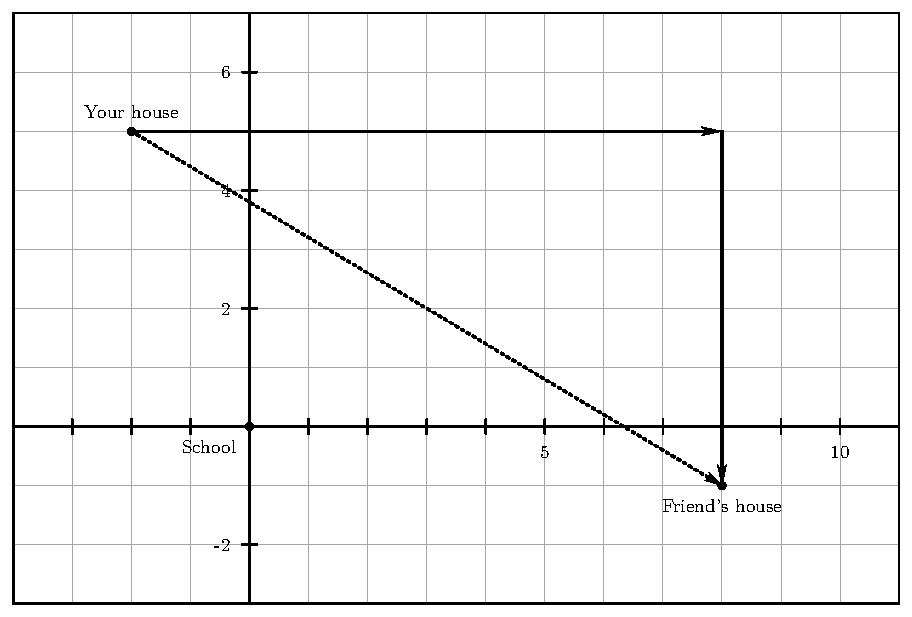
\includegraphics[width=.92\linewidth]{../figures/fhsm_2009_p_7_1.pdf}
  \end{center}

  \item[Student 3:] Wait a minute---you just drew a right triangle, because the streets are perpendicular.
  \item[Student 4:] So that means we could use the Pythagorean theorem: $10^2+6^2=c^2$, so $c=\sqrt{136}$.
  \item[Student 2:] But how many blocks would that be?
  \item[Student 3:] Shouldn't the distance be between eleven and twelve blocks, since $121 < 136 < 144$? Actually, it's probably closer to twelve blocks, since $136$ is much closer to $144$.
  
  (The teacher then extends the discussion to consider other examples and finally to develop a general formula.)
\end{description}}
}
{
\VI{
\begin{description}
  \item[Giáo viên:] Chúng ta hãy xem một tình huống trong đó ta cần tìm khoảng cách giữa hai vị trí trên bản đồ. Giả sử bản đồ này thể hiện trường học của em; nhà của em nằm cách trường hai dãy phố về phía tây và năm dãy phố về phía bắc, còn nhà của bạn em nằm cách trường tám dãy phố về phía đông và một dãy phố về phía nam. Nếu thành phố có hệ thống các con phố vuông góc và cách đều nhau, thì chúng ta sẽ phải đi bao nhiêu dãy phố để đi từ nhà em đến nhà bạn em?
  \item[Học sinh 1:] Ờ, mình phải đi mười dãy phố về phía đông và sáu dãy phố về phía nam, vậy chắc là mười sáu dãy phố, đúng không ạ?
  \item[Giáo viên:] Bây giờ, giả sử em có thể dùng trực thăng để bay thẳng đến nhà bạn. Làm thế nào để ta tìm được khoảng cách ``đường chim bay''? Hãy làm việc theo nhóm để thiết lập một hệ trục tọa độ và biểu diễn đường đi trên các con phố từ nhà em đến nhà bạn. Sau đó, hãy tính khoảng cách trực tiếp giữa hai ngôi nhà nếu em được bay thẳng.
  \item[Học sinh 1:] Nếu dùng trường học làm gốc tọa độ thì sao ạ? Khi đó, nhà em sẽ ở $(-2, 5)$, còn nhà bạn em ở $(8, -1)$, đúng không?
  \item[Học sinh 2:] Nghe hợp lý đó. Đây này, chúng ta vẽ đường đi theo các con phố nối hai ngôi nhà, rồi sau đó vẽ đoạn thẳng nối hai ngôi nhà.
  \item[Học sinh 1:] Hay là mình đo chiều dài một dãy phố rồi dùng thước để tính khoảng cách?
  
    \begin{center}
      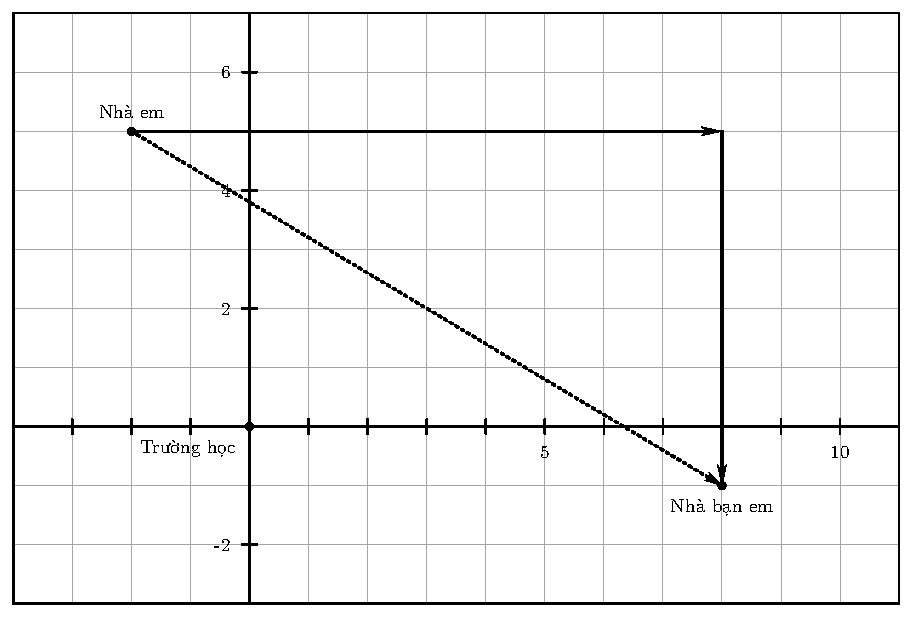
\includegraphics[width=.92\linewidth]{../figures/fhsm_2009_p_7_1_vi.pdf}
    \end{center}

  \item[Học sinh 3:] Khoan đã, bạn vừa vẽ một tam giác vuông mà, vì các con phố vuông góc với nhau.
  \item[Học sinh 4:] Vậy tức là ta có thể dùng định lý Pythagoras: $10^2 + 6^2 = c^2$, nên $c = \sqrt{136}$.
  \item[Học sinh 2:] Nhưng như vậy là bao nhiêu dãy phố?
  \item[Học sinh 3:] Chẳng phải khoảng cách phải nằm giữa 11 và 12 dãy phố sao, vì $121 < 136 < 144$? Thực ra, nó có lẽ gần 12 dãy phố hơn, vì $136$ gần $144$ hơn nhiều.
  
  (Giáo viên sau đó mở rộng thảo luận sang các ví dụ khác và cuối cùng xây dựng công thức tổng quát.)
\end{description}}
}
{
\NOTE{Kịch bản này cho thấy một lớp học nơi học sinh được đặt vào trung tâm của quá trình tư duy toán học, thay vì đứng ngoài quan sát giáo viên trình bày công thức. Điểm xuất phát không phải là ký hiệu hay quy trình, mà là một tình huống quen thuộc trong đời sống: tìm khoảng cách giữa hai vị trí trên bản đồ thành phố. Chính sự quen thuộc này tạo điều kiện để học sinh bắt đầu hiểu, bởi các em có thể hình dung, ước lượng và dự đoán trước khi đi vào biểu diễn toán học.

Ở giai đoạn đầu, học sinh tự nhiên đưa ra khoảng cách theo ``đường phố'', tức là tổng quãng đường phải đi dọc theo các con phố vuông góc. Cách trả lời này không sai, nhưng nó phản ánh một cách hiểu còn gắn với trải nghiệm đời sống. Giáo viên không bác bỏ, mà mở rộng tình huống bằng một câu hỏi mới: nếu có thể đi thẳng thì sao? Câu hỏi này buộc học sinh phải tái cấu trúc vấn đề, từ đó chuyển sang một kiểu biểu diễn khác.

Khi học sinh tự chọn trường học làm gốc tọa độ và xác định vị trí hai ngôi nhà bằng tọa độ, một bước hiểu quan trọng đã diễn ra: các em không chỉ dùng hệ trục tọa độ, mà hiểu vì sao việc đó có ý nghĩa trong tình huống này. Việc vẽ đường đi trên phố và đoạn thẳng nối hai ngôi nhà tạo ra một cầu nối trực quan giữa bối cảnh thực và mô hình toán học.

Khoảnh khắc học sinh nhận ra rằng hình vẽ tạo thành một tam giác vuông là điểm xoay của toàn bộ hoạt động. Ở đây, luận xuất hiện một cách tự nhiên: từ quan sát ``các con phố vuông góc'' đến kết luận ``đây là tam giác vuông'', rồi đến việc vận dụng định lý Pythagoras. Không có công thức nào được nhắc lại từ trí nhớ; thay vào đó, công thức khoảng cách được tái tạo như một hệ quả hợp lý của lập luận hình học.

Đáng chú ý là quá trình này không dừng lại ở việc tính toán chính xác, mà còn bao gồm suy luận xấp xỉ khi học sinh so sánh 136 với các bình phương lân cận. Điều này cho thấy luận không chỉ là suy luận hình thức, mà còn bao hàm khả năng đánh giá, ước lượng và diễn giải kết quả trong bối cảnh cụ thể.

Toàn bộ kịch bản minh họa rõ ràng sự khác biệt giữa hai cách dạy: trong kịch bản thứ nhất, học sinh cố gắng nhớ công thức mà không hiểu; trong kịch bản này, công thức xuất hiện như kết quả tự nhiên của một chuỗi luận và hiểu đan xen. Kiến thức không còn là thứ được ``trao tay'', mà là thứ được học sinh tự xây dựng thông qua hoạt động tư duy. Chính sự khác biệt này làm cho công thức khoảng cách trở nên có ý nghĩa, dễ nhớ và có khả năng chuyển giao sang những tình huống khác.}
}

\TriPara
{
\EN{By having her students approach the distance formula from a reasoning-and-sense-making perspective the second year, the teacher increases their understanding of the formula and why it is true, increasing the likelihood that they will be able to retrieve, or quickly recreate, the formula at a later time.}
}
{
\VI{Bằng việc để học sinh tiếp cận công thức khoảng cách từ một góc nhìn dựa trên luận và hiểu ở năm học thứ hai, giáo viên đã làm tăng sự hiểu biết của các em về công thức cũng như vì sao công thức đó đúng, qua đó nâng cao khả năng để sau này các em có thể nhớ lại, hoặc nhanh chóng tự tái tạo, công thức ấy khi cần.}
}
{
\NOTE{}
}

\ParallelSection
{Conclusion}
{Kết luận}
{}

\TriPara
{
\EN{Reasoning and sense making are the cornerstones of mathematics. Restructuring the high school mathematics program around them enhances students' development of both the content and process knowledge they need to be successful in their continuing study of mathematics and in their lives.}
}
{
\VI{Luận và hiểu là những viên đá nền tảng của toán học. Việc tái cấu trúc chương trình toán trung học phổ thông xoay quanh hai năng lực này sẽ thúc đẩy sự phát triển của học sinh cả về tri thức nội dung lẫn tri thức quá trình---những điều các em cần để thành công trong việc học toán ở các bậc tiếp theo và trong cuộc sống.}
}
{
\NOTE{Khép lại toàn bộ Chương 1 bằng một khẳng định dứt khoát: luận và hiểu không phải những năng lực bổ sung bên cạnh nội dung toán học, mà là nền tảng làm cho nội dung ấy thực sự trở thành toán học. Từ đó, NCTM rút ra hệ quả ở bình diện chương trình: toán trung học phổ thông không thể tiếp tục được tổ chức chủ yếu quanh danh sách chủ đề và quy trình, mà phải được tái cấu trúc quanh luận và hiểu.

Sự tái cấu trúc này không nhằm thay thế tri thức nội dung bằng các quá trình, mà nhằm làm cho hai phương diện ấy phát triển cùng nhau. Khi luận và hiểu trở thành điểm tựa, học sinh không chỉ học được các khái niệm và kết quả, mà còn hình thành được những cách thức làm việc với toán học một cách có ý nghĩa và bền vững. Vì vậy, đây không chỉ là lời kết của Chương 1, mà còn là mệnh đề trung tâm chi phối toàn bộ lập trường của cuốn sách.}
}

% ==========
% CHAPTER 2
% ==========

\ParallelChapter
{Reasoning Habits}
{Thói quen luận}
{}

\TriPara
{
\EN{
  \begin{flushright}
  \emph{Reasoning and sense making should be a part of the mathematics classroom every day.}
  \end{flushright}}
}
{
\VI{
  \begin{flushright}
  \emph{Luận và hiểu phải là một phần của lớp học toán mỗi ngày.}
  \end{flushright}}
}
{
\NOTE{Xác lập lập trường trung tâm của chương: luận và hiểu không phải mục tiêu phụ trợ, mà phải được tích hợp vào thực hành dạy học toán hằng ngày.}
}

\TriPara
{
\EN{A focus on reasoning and sense making implies that ``covering'' mathematical topics is not enough. Students also need to experience and develop mathematical reasoning habits (cf. Cuoco, Goldenberg, and Mark [1996]; Driscoll [1999]; Pólya [1952, 1957]; Schoenfeld [1983]; Harel and Sowder [2005]). A \emph{reasoning habit} is a productive way of thinking that becomes common in the processes of mathematical inquiry and sense making. The following list of reasoning habits illustrates the types of thinking that should become routine and fully expected in the classroom culture of all mathematics classes across all levels of high school.}
}
{
\VI{Một trọng tâm đặt vào luận và hiểu hàm ý rằng chỉ ``dạy cho hết'' các chủ đề toán học là không đủ. Học sinh còn cần được trải nghiệm và phát triển các thói quen luận trong toán học (xem Cuoco, Goldenberg, and Mark [1996]; Driscoll [1999]; Pólya [1952, 1957]; Schoenfeld [1983]; Harel and Sowder [2005]). Một \emph{thói quen luận} là một cách tư duy hiệu quả, dần trở nên quen thuộc trong các quá trình tìm tòi toán học và hiểu. Danh sách các thói quen luận dưới đây minh họa những kiểu tư duy cần trở thành thông lệ và được xem là điều đương nhiên trong văn hóa lớp học của mọi lớp toán ở tất cả các cấp độ trung học phổ thông.}
}
{
\NOTE{Ở đây, điều bị bác bỏ không phải là nội dung toán học, mà là quan niệm cho rằng chỉ cần ``dạy hết nội dung'' thì đã đủ. Nếu lấy luận và hiểu làm trọng tâm, học sinh phải thường xuyên được sống trong những cách nghĩ có năng suất của hoạt động toán học. Vì vậy, các thói quen luận không phải phần phụ trợ, mà là một chuẩn thường nhật của văn hóa lớp học toán ở bậc THPT.}
}

\TriPara
{
\EN{Approaching the list as a new set of topics to be taught in an already crowded curriculum is not likely to have the desired effect. Instead, attention to reasoning habits needs to be integrated within the curriculum to ensure that students both understand and can use what they are taught.}
}
{
\VI{Tiếp cận danh sách các thói quen luận như một tập hợp chủ đề mới cần dạy trong một chương trình học vốn đã quá tải sẽ khó mang lại hiệu quả mong muốn. Thay vào đó, sự chú tâm đối với các thói quen luận cần được tích hợp vào ngay trong chương trình để bảo đảm rằng học sinh vừa hiểu vừa có thể sử dụng được những gì các em được học.}
}
{
\NOTE{}
}

\TriPara
{
\EN{
\begin{itemize}
  \item  \emph{Analyzing a problem}, for example,
  \begin{itemize}
    \item \emph{identifying relevant} mathematical \emph{concepts, procedures, or representations} that reveal important information about the problem and contribute to its solution (for example, choosing a model for simulating a random experiment);
    \item \emph{defining relevant variables and conditions} carefully, including units if appropriate;
    \item \emph{seeking patterns and relationships} (for example, systematically examining cases or creating displays for data);
    \item \emph{looking for hidden structure} (for example, drawing auxiliary lines in geometric figures or finding equivalent forms of expressions that reveal different aspects of a problem);
    \item \emph{considering special cases or simpler analogs};
    \item \emph{applying previously learned concepts} to new problem situations, adapting and extending as necessary;
    \item \emph{making preliminary deductions and conjectures}, including predicting what a solution to a problem might involve or putting constraints on solutions; and
    \item \emph{deciding whether a statistical approach is appropriate}.
  \end{itemize}
  \item \emph{Implementing a strategy}, for example,
  \begin{itemize}
    \item \emph{making purposeful use of procedures};
    \item \emph{organizing the solution}, including calculations, algebraic manipulations, and data displays;
    \item \emph{making logical deductions} based on current progress, verifying conjectures, and extending initial findings; and
    \item \emph{monitoring progress toward a solution}, including reviewing a chosen strategy and other possible strategies generated by oneself or others.
  \end{itemize}
  \item \emph{Seeking and using connections} across different mathematical domains, different contexts, and different representations.
  \item \emph{Reflecting on a solution} to a problem, for example,
  \begin{itemize}
    \item \emph{interpreting a solution} and how it answers the problem, including making decisions under uncertain conditions;
    \item \emph{considering the reasonableness of a solution}, including whether any numbers are reported at an unreasonable level of accuracy;
    \item \emph{revisiting initial assumptions} about the nature of the solution, including being mindful of special cases and extraneous solutions;
    \item \emph{justifying or validating a solution}, including through proof or inferential reasoning;
    \item \emph{recognizing the scope of inference} for a statistical solution;
    \item \emph{reconciling different approaches} to solving the problem, including those proposed by others;
    \item \emph{refining arguments} so that they can be effectively communicated; and
    \item \emph{generalizing a solution} to a broader class of problems and looking for connections with other problems.
  \end{itemize}
\end{itemize}
}
}
{
\VI{
  \begin{itemize}
    \item \emph{Phân tích bài toán}, chẳng hạn:
    \begin{itemize}
      \item \emph{xác định các khái niệm, thủ tục, hoặc biểu diễn toán học thích đáng}---những yếu tố làm lộ ra thông tin quan trọng của bài toán và đóng góp vào lời giải (ví dụ, chọn một mô hình để mô phỏng một thí nghiệm ngẫu nhiên);
      \item \emph{xác định cẩn thận các biến và điều kiện thích đáng}, bao gồm cả đơn vị đo nếu cần;
      \item \emph{tìm kiếm các mẫu hình và quan hệ} (ví dụ, xét các trường hợp một cách có hệ thống, hoặc tạo biểu đồ cho dữ liệu);
      \item \emph{tìm kiếm cấu trúc ẩn} (ví dụ: kẻ đường phụ trong hình học hoặc tìm các dạng tương đương của biểu thức để làm lộ ra những khía cạnh khác nhau của bài toán);
      \item \emph{xét các trường hợp đặc biệt hoặc những trường hợp tương tự đơn giản hơn};
      \item \emph{vận dụng các khái niệm đã học} vào tình huống bài toán mới, điều chỉnh và mở rộng khi cần thiết;
      \item \emph{đưa ra những suy diễn và phỏng đoán sơ bộ}, bao gồm dự đoán lời giải có thể cần những gì hoặc đặt ra các ràng buộc cho lời giải; và
      \item \emph{quyết định liệu một cách tiếp cận thống kê có phù hợp hay không}.
    \end{itemize}
    \item \emph{Triển khai chiến lược}, chẳng hạn:
    \begin{itemize}
      \item \emph{vận dụng có chủ đích các thủ tục};
      \item \emph{tổ chức lời giải}, bao gồm các phép tính, biến đổi đại số và biểu diễn dữ liệu;
      \item \emph{thực hiện những suy diễn có tính luận lý} dựa trên tiến triển hiện tại, kiểm tra các phỏng đoán, và mở rộng những kết quả ban đầu; và
      \item \emph{theo dõi tiến trình đi đến lời giải}, bao gồm xem xét lại chiến lược đã chọn và các chiến lược khả dĩ khác do mình hoặc người khác đề xuất.
    \end{itemize}
    \item \emph{Tìm kiếm và sử dụng các kết nối} giữa các miền toán học khác nhau, giữa các bối cảnh khác nhau, và giữa các biểu diễn khác nhau.
    \item \emph{Phản tư về lời giải}, chẳng hạn:
    \begin{itemize}
      \item \emph{diễn giải lời giải} và cách nó trả lời bài toán, bao gồm việc đưa ra quyết định trong những điều kiện không chắc chắn;
      \item \emph{xem xét tính hợp lý của lời giải}, bao gồm việc đánh giá xem các con số được báo cáo có mức chính xác hợp lý hay không;
      \item \emph{xem lại các giả định ban đầu} về bản chất của lời giải, bao gồm việc chú ý đến các trường hợp đặc biệt và nghiệm ngoại lai;
      \item \emph{biện minh hoặc kiểm chứng một lời giải}, bao gồm thông qua chứng minh hoặc lập luận suy diễn;
      \item \emph{nhận diện phạm vi suy luận} đối với một lời giải thống kê; 
      \item \emph{dung hòa các cách tiếp cận khác nhau} để giải bài toán, bao gồm cả những cách do người khác đề xuất;
      \item \emph{tinh chỉnh lập luận} để có thể truyền đạt hiệu quả; và
      \item \emph{khái quát hóa lời giải} sang một lớp bài toán rộng hơn và tìm kiếm các kết nối với những bài toán khác.
    \end{itemize}
  \end{itemize}
}
}
{
\NOTE{Các thói quen luận không phải là những kỹ thuật rời rạc, mà là những nếp hoạt động trí tuệ cần hiện diện xuyên suốt quá trình học: từ phân tích một bài toán, triển khai một chiến lược, tìm kiếm và sử dụng các kết nối, đến phản tư về một lời giải. Trọng tâm không nằm ở việc làm cho xong bài toán, mà ở việc học sinh dần biết làm rõ bản chất của vấn đề, điều khiển tiến trình giải, nối các ý tưởng toán học trong những bối cảnh và biểu diễn khác nhau, rồi xem xét lại lời giải để đánh giá, kiểm tra và mở rộng nó khi cần. Qua đó, luận được đặt như một chuẩn thường nhật của văn hóa lớp học toán, chứ không phải một yêu cầu phụ thêm sau khi đã ``dạy hết'' nội dung.}
}

\TriPara
{
\EN{Many of these reasoning habits could be construed to fit in more than one category, and students are expected to move naturally among various reasoning habits as they are needed. Section 2 of this publication offers examples of how reasoning habits can be promoted in the high school classroom, with specific references to the reasoning habits listed above.}
}
{
\VI{Nhiều thói quen luận trong số này có thể được xem là phù hợp với hơn một nhóm, và học sinh được kỳ vọng sẽ chuyển đổi một cách tự nhiên giữa các thói quen luận khác nhau khi cần. Phần 2 của ấn phẩm này đưa ra các ví dụ về cách thúc đẩy các thói quen luận trong lớp học toán trung học phổ thông, với các tham chiếu cụ thể đến những thói quen luận đã liệt kê ở trên.}
}
{
\NOTE{Các thói quen luận không được hiểu như những nhóm tách biệt với ranh giới cứng. Một thói quen cụ thể có thể xuất hiện trong nhiều bối cảnh khác nhau, và trong thực hành, học sinh được kỳ vọng sẽ chuyển đổi linh hoạt giữa các thói quen luận tùy theo yêu cầu của bài toán.}
}

\ParallelSection
  {Progression of Reasoning}
  {Tiến triển của luận}
  {Cách dịch này, Tiến trình phát triển của các thói quen luận, phản ánh đúng hai tầng ý nghĩa của tiêu đề gốc \emph{Progression of Reasoning} trong ngữ cảnh Chương 2.

  Thứ nhất, từ ``tiến trình'' được chọn để làm nổi bật ý tưởng \emph{progression} như một sự phát triển có trật tự và có mức độ, chứ không phải sự thay đổi ngẫu nhiên hay phát triển chung chung. Tác giả không bàn về sự ``trưởng thành'' của luận theo nghĩa tâm lý học, mà về cách các kỳ vọng đối với luận được nâng dần trong thực hành dạy học.

  Thứ hai, việc bổ sung ``các thói quen luận'' giúp neo tiêu đề này trực tiếp vào mạch nội dung vừa được xây dựng ở phần trước. Chương 2 không xem luận như một năng lực đơn khối, mà như một tập hợp các thói quen có thể được quan sát, nuôi dưỡng và phát triển dần theo thời gian. Do đó, ``tiến trình phát triển'' ở đây chính là tiến trình trong đó các thói quen luận trở nên ngày càng tinh vi, chặt chẽ và được kỳ vọng cao hơn trong lớp học toán trung học phổ thông.

  Cách dịch này vì vậy tránh được hai cách hiểu sai phổ biến: một là hiểu \emph{progression} như lý thuyết phát triển nhận thức nói chung; hai là hiểu luận như một kỹ năng tách rời khỏi các thói quen tư duy cụ thể.}

\TriPara
{
\EN{When reasoning is interwoven with sense making, and when teachers provide the necessary support and formative feedback, students can be expected to demonstrate growing levels of formality in their reasoning in the classroom, in their oral and written work, and in assessments throughout the high school years. Reasoning and sense making in the high school mathematics classroom require increasing levels of understanding, as outlined in the following:

\begin{description}
  \item[empirical] --- the role of empirical evidence that supports, but does not justify, a conjecture---``it works in a number of cases'';
  \item[preformal] --- the role of intuitive explanations and partial arguments that lend insight into what is happening; and
  \item[formal] --- the role of formal argumentation (based on logic) in determining mathematical certainty (proof) or in making statistical inferences.
\end{description}
}
}
{
\VI{Khi luận được đan xen với hiểu, và khi giáo viên cung cấp sự hỗ trợ cần thiết cùng phản hồi hình thành, học sinh có thể được kỳ vọng sẽ thể hiện những mức độ ngày càng tăng về tính hình thức trong luận của mình---trong lớp học, trong sản phẩm nói và viết, và trong các hình thức đánh giá---xuyên suốt những năm trung học phổ thông. Luận và hiểu trong lớp học toán trung học phổ thông đòi hỏi mức độ hiểu biết ngày càng cao, như được phác thảo dưới đây:

\begin{description}
  \item[thực nghiệm] --- vai trò của bằng chứng thực nghiệm đó là hỗ trợ, nhưng không đủ để biện minh cho một giả thuyết---``nó đúng trong một số trường hợp'';
  \item[tiền hình thức] --- vai trò của các giải thích trực giác và các lập luận bộ phận đó là giúp soi sáng điều đang diễn ra; và
  \item[hình thức] --- vai trò của lập luận hình thức (dựa trên luận lý) trong việc xác lập tính chắc chắn toán học (chứng minh) hoặc trong việc đưa ra suy luận thống kê.
\end{description}
}
}
{
\NOTE{Đoạn này xác lập một trục phát triển cho luận trong lớp học toán trung học phổ thông: từ thực nghiệm, qua tiền hình thức, đến hình thức. Điều được nhấn mạnh không phải là thay thế mức trước bằng mức sau, mà là học sinh dần đạt tới những mức độ ngày càng cao về tính hình thức trong luận của mình, với điều kiện luận luôn gắn với hiểu và được nâng đỡ bằng hỗ trợ cùng phản hồi hình thành từ phía giáo viên. Qua đó, sách bác bỏ cách nhìn xem chứng minh hay suy luận thống kê là những năng lực chỉ xuất hiện ở điểm cuối; chúng phải được chuẩn bị dần từ những cách nhận định còn dựa vào trường hợp, trực giác và lập luận bộ phận.}
}

\TriPara
{
\EN{Thus, these levels show progress from less formal reasoning to more formal reasoning. However, each level has value. Students may continually shift among these levels, even within the same mathematical context. This shifting among levels is not only expected but desirable as students make sense of the context and reason their way to a conclusion. However, teachers play an essential role in encouraging students to explore more sophisticated levels of reasoning and sense making.}
}
{
\VI{Do đó, các mức độ này cho thấy sự tiến bộ từ luận ít hình thức hơn đến luận mang tính hình thức hơn. Tuy vậy, mỗi mức độ đều có giá trị riêng. Học sinh có thể liên tục chuyển đổi giữa các mức độ này, thậm chí trong cùng một bối cảnh toán học. Sự chuyển đổi này không chỉ được kỳ vọng mà còn được xem là điều đáng mong muốn, vì nó phản ánh quá trình học sinh hiểu đối với bối cảnh và luận để đi đến kết luận. Tuy nhiên, giáo viên đóng vai trò thiết yếu trong việc khuyến khích học sinh khám phá các mức luận và hiểu tinh vi hơn.}
}
{
\NOTE{}
}

\TriPara
{
\EN{Formal argumentation includes both the ability of students to create meaningful chains of logical reasoning based on certain assumptions, definitions, and prior results, as well as the ability to read and evaluate reasoning given by others. The ability to determine the validity of an argument is important, as is an understanding of what the argument says about the ideas under consideration.}
}
{
\VI{Lập luận hình thức bao gồm cả khả năng của học sinh trong việc tạo ra các chuỗi luận có tính luận lý có ý nghĩa dựa trên những giả định, định nghĩa và các kết quả đã biết, cũng như khả năng đọc và đánh giá luận do người khác đưa ra. Khả năng xác định tính hợp lệ của một lập luận là quan trọng, cũng như việc hiểu được lập luận đó nói gì về các ý tưởng đang được xem xét.}
}
{
\NOTE{}
}

\ParallelSection
  {Developing Reasoning Habits in the Classroom}
  {Phát triển các thói quen luận trong lớp học}
  {}

\TriPara
{
\EN{Teachers can help students progress to higher levels of reasoning through judicious selection of tasks and the use of probing questions. Students can then learn to analyze their approach to solving problems, recognize the strengths and shortcomings of their current approach, and use the power of more formal reasoning to better formulate and justify mathematical conclusions. The continuing development of mathematical reasoning habits should be a priority in the high school classroom. The following is a preliminary list of tips for developing these habits.}
}
{
\VI{Giáo viên có thể giúp học sinh tiến tới các mức luận tinh vi hơn thông qua việc lựa chọn nhiệm vụ một cách thận trọng và sử dụng các câu hỏi gợi mở. Khi đó, học sinh có thể học cách phân tích cách tiếp cận của chính mình trong việc giải bài toán, nhận ra điểm mạnh và hạn chế của cách tiếp cận hiện tại, và sử dụng sức mạnh của luận mang tính hình thức hơn để xây dựng và biện minh các kết luận toán học tốt hơn. Việc phát triển liên tục các thói quen luận cần được xem là một ưu tiên trong lớp học toán trung học phổ thông. Dưới đây là một danh sách ban đầu các gợi ý nhằm phát triển những thói quen này.}
}
{
\NOTE{}
}

\TriPara
{
\EN{
  \begin{itemize}
    \item Provide tasks that require students to figure things out for themselves.
    \item Ask students to restate the problem in their own words, including any assumptions they have made.
    \item Give students time to analyze a problem intuitively, explore the problem further by using models, and then proceed to a more formal approach.
    \item Resist the urge to tell students how to solve a problem when they become frustrated; find other ways to support students as they think and work.
    \item Ask students questions that will prompt their thinking---for example, ``Why does this work?'' or ``How do you know?''
    \item Provide adequate wait time after a question for students to formulate their own reasoning.
    \item Encourage students to ask probing questions of themselves and one another.
    \item Expect students to communicate their reasoning to their classmates and the teacher, orally and in writing, through using proper mathematical vocabulary.
    \item Highlight exemplary explanations, and have students reflect on what makes them effective.
    \item Establish a classroom climate in which students feel comfortable sharing their mathematical arguments and critiquing the arguments of others in a productive manner.
  \end{itemize}
}
}
{
\VI{
  \begin{itemize}
    \item Cung cấp các nhiệm vụ buộc học sinh phải tự mình tìm ra cách tiếp cận.
    \item Yêu cầu học sinh diễn đạt lại bài toán bằng lời của chính mình, bao gồm cả những giả định mà các em đã đưa ra.
    \item Cho học sinh thời gian để phân tích bài toán một cách trực giác, khám phá sâu hơn bằng các mô hình, rồi sau đó mới chuyển sang cách tiếp cận mang tính hình thức hơn.
    \item Kiềm chế việc chỉ cho học sinh cách giải khi các em cảm thấy thất vọng; thay vào đó, hãy tìm những cách hỗ trợ khác trong khi học sinh đang suy nghĩ và làm việc.
    \item Đặt các câu hỏi gợi mở nhằm thúc đẩy luận của học sinh---chẳng hạn, ``Vì sao cách này hoạt động?” hoặc “Làm sao em biết điều đó?''.
    \item Dành thời gian chờ hợp lý sau mỗi câu hỏi để học sinh có thể tự hình thành luận của mình.
    \item Khuyến khích học sinh đặt các câu hỏi gợi mở cho chính mình và cho bạn cùng lớp.
    \item Kỳ vọng học sinh trình bày luận của mình với bạn học và với giáo viên, cả bằng lời nói và bằng văn viết, thông qua việc sử dụng đúng thuật ngữ toán học.
    \item Nêu bật các lời giải thích mẫu mực và yêu cầu học sinh phản tư về điều gì khiến chúng trở nên hiệu quả.
    \item Xây dựng một môi trường lớp học nơi học sinh cảm thấy thoải mái chia sẻ các lập luận toán học của mình và phê bình lập luận của người khác theo cách mang tính xây dựng.
  \end{itemize}
}
}
{
\NOTE{Danh sách này quy tụ những thực hành lớp học có tác dụng nuôi dưỡng luận ở học sinh. Điểm chung của chúng là không đẩy học sinh thẳng tới lời giải, mà tạo điều kiện để các em tự phân tích tình huống, tự diễn đạt cách hiểu của mình, tự nêu giả định, tự chất vấn, rồi từng bước chuyển từ trực giác và mô hình sang cách tiếp cận chặt chẽ hơn.

Ở đây, luận không được xem như một sản phẩm xuất hiện ở cuối cùng, mà như một hoạt động được hình thành ngay trong quá trình học sinh nghĩ, nói, viết, hỏi và phản biện. Vì vậy, vai trò của giáo viên không phải trước hết là chỉ cách làm, mà là thiết kế nhiệm vụ, đặt câu hỏi, giữ nhịp chờ, và xây dựng một môi trường lớp học đủ an toàn để lập luận có thể được đưa ra, được xem xét, và được cải thiện.}
}

\TriPara
{
\EN{Teachers should refer to other resources for specific tasks, suggestions for questioning techniques, and so forth. NCTM and other professional organizations offer a number of valuable resources, both in print and online. Additional teaching ideas related to reasoning and sense making are also presented in more detail in the topic books that support this publication.}
}
{
\VI{Giáo viên nên tham khảo các nguồn tư liệu khác để tìm những nhiệm vụ cụ thể, các gợi ý về kỹ thuật đặt câu hỏi, và các tài liệu liên quan. NCTM cùng nhiều tổ chức nghề nghiệp khác cung cấp nhiều nguồn tài liệu giá trị, cả dưới dạng in ấn lẫn trực tuyến. Những ý tưởng dạy học bổ sung liên quan đến luận và hiểu cũng được trình bày chi tiết hơn trong các sách chuyên đề hỗ trợ cho ấn phẩm này.}
}
{
\NOTE{}
}

\ParallelSection
  {Reasoning as the Foundation of Mathematical Competence}
  {Luận như nền tảng của năng lực toán học}
  {}

\TriPara
{
\EN{Reasoning and sense making are inherent in developing mathematical competence, as discussed in \emph{Adding It Up} (Kilpatrick, Swafford, and Findell 2001); see figure 2.1. Sense making and conceptual understanding are closely interrelated. Procedural fluency includes learning with understanding and knowing which procedure to choose, when to choose it, and for what purpose. In the absence of reasoning, students may carry out procedures correctly but may also capriciously invoke incorrect or baseless rules, such as ``the square root of a sum is the sum of the square roots.'' They come to view procedures as steps they are told to do rather than a series of steps chosen for a specific purpose and based on mathematical principles. Without developing an understanding of procedures rooted in reasoning and sense making, students may be able to correctly perform those procedures but may think of them only as a list of ``tricks.'' As a result, they may have difficulty selecting an appropriate procedure to use in a given problem, or their seeming competence with simple tasks may evaporate in more complicated situations. Genuine procedural fluency requires both mastering technical skills and developing the understanding needed for using them appropriately. Strategic competence and adaptive reasoning are both directly addressed in the reasoning habits. }
}
{
\VI{Luận và hiểu là những thành tố vốn có trong việc phát triển năng lực toán học, như đã được bàn trong \emph{Adding It Up} (Kilpatrick, Swafford, và Findell 2001); xem hình 2.1. Hiểu và sự lĩnh hội khái niệm có quan hệ gắn bó chặt chẽ với nhau. Sự trôi chảy về thủ tục bao gồm việc học một cách thông hiểu, cũng như biết chọn thủ tục nào, khi nào chọn, và nhằm mục đích gì. Khi thiếu luận, học sinh có thể thực hiện đúng các thủ tục, nhưng cũng có thể tùy tiện viện đến những quy tắc sai hoặc vô căn cứ, chẳng hạn như ``căn bậc hai của một tổng bằng tổng các căn bậc hai.'' Các em dần xem các thủ tục như những bước được bảo phải làm, thay vì như một chuỗi bước được lựa chọn cho một mục đích xác định và dựa trên các nguyên lý toán học. Nếu không phát triển sự thông hiểu về các thủ tục trên nền của luận và hiểu, học sinh có thể thực hiện đúng các thủ tục ấy nhưng chỉ xem chúng như một danh sách các ``mẹo''. Hệ quả là các em có thể gặp khó khăn khi phải chọn một thủ tục thích hợp cho một bài toán cụ thể, hoặc năng lực tưởng như vững vàng của các em trong những nhiệm vụ đơn giản lại tan biến khi gặp những tình huống phức tạp hơn. Sự trôi chảy về thủ tục đích thực đòi hỏi đồng thời việc nắm vững các kĩ năng kĩ thuật và phát triển sự thông hiểu cần thiết để sử dụng chúng một cách thích đáng. Năng lực chiến lược và năng lực suy luận thích ứng đều được các thói quen luận trực tiếp đề cập đến.}
}
{
\NOTE{Thuật ngữ ``\emph{adaptive reasoning}'', vốn dễ gây nhầm lẫn với thuật ngữ lập trường ``luận'' được giữ xuyên suốt ấn phẩm. Theo khung năng lực trong \emph{Adding It Up} (Kilpatrick, Swafford, Findell 2001), adaptive reasoning không phải là một biến thể hay cấp độ của luận theo nghĩa lập trường, mà là tên gọi một năng lực cụ thể, đặt song song với \emph{procedural fluency} và \emph{strategic competence}.

Vì vậy, ``adaptive reasoning'' được dịch là ``\emph{năng lực suy luận thích ứng}'', nhằm phản ánh đúng cấp độ khái niệm và tránh nhập nhằng với thuật ngữ luận đang được dùng để chỉ lập trường tư duy chung của cuốn sách. Cách dịch này giúp giữ rõ ranh giới giữa luận như một lập trường xuyên suốt và adaptive reasoning như một thành phần trong cấu trúc năng lực toán học.}
}

\TriFigure
  {../figures/fhsm_2009_p12_f1.pdf}
  {../figures/fhsm_2009_p12_f1_vi.pdf}
  {The strands of mathematical proficiency from Adding It Up (Kilpatrick, Swafford, and Findell 2001)}
  {Mô tả các sợi năng lực toán học trong Adding It Up. (Kilpatrick, Swafford, and Findell 2001)}
  {fig:fig_2.1}


\TriPara
{
\EN{The development of a ``productive disposition'' (Kilpatrick, Swafford, and Findell 2001) is a high priority of all school mathematics programs. When students achieve this goal, they view mathematics as a reasoning and sense-making enterprise. This goal can be achieved only if students personally engage in mathematical reasoning and sense making as they learn mathematics content.}
}
{
\VI{Sự phát triển ``khuynh hướng tích cực'' đối với toán học (Kilpatrick, Swafford và Findell 2001) là một ưu tiên hàng đầu của mọi chương trình toán học ở trường phổ thông. Khi đạt được mục tiêu này, học sinh xem toán học như một hoạt động luận và hiểu. Mục tiêu này chỉ có thể đạt được nếu học sinh tự thân tham gia vào luận và hiểu trong quá trình học nội dung toán học.}
}
{
\NOTE{Khuynh hướng tích cực đối với toán học không thể được tạo ra bằng lời khuyên hay động viên bên ngoài. Học sinh chỉ có thể dần xem toán học là điều có thể hiểu, có thể lý giải và đáng để theo đuổi khi chính các em trực tiếp tham gia vào luận và hiểu trong quá trình học. Vì thế, thái độ của học sinh đối với toán học không tách rời cách toán học được sống trong lớp học.}
}

\ParallelSection
  {Statistical Reasoning}
  {Luận thống kê}
  {}

\TriPara
{
\EN{Statistical reasoning involves making interpretations based on, and inferences from, data. Statistics furnishes tools for investigating questions by providing strategies for collecting useful data, methods for analyzing the data, and unique perspectives for interpreting the meaning of the data within the context of the problem. The need for statistics arises from “the omnipresence of Conceptual understanding variability” in data (Cobb and Moore 1997, p. 801), and statistical reasoning uses a combination of ideas from both data and chance in seeking to understand that variability. Such notions as distribution, center, spread, association, uncertainty, randomness, sampling, and statistical experiments are foundational concepts underlying the development of statistical reasoning.}
}
{
\VI{Luận thống kê bao gồm việc đưa ra những diễn giải dựa trên dữ liệu và những suy luận rút ra từ dữ liệu. Thống kê cung cấp các công cụ để khảo sát các câu hỏi bằng cách cung cấp những chiến lược thu thập dữ liệu hữu ích, những phương pháp phân tích dữ liệu, và những góc nhìn riêng để diễn giải ý nghĩa của dữ liệu trong bối cảnh của bài toán. Nhu cầu đối với thống kê nảy sinh từ ``sự hiện diện khắp nơi của tính biến thiên'' trong dữ liệu (Cobb và Moore 1997, tr. 801), và luận thống kê sử dụng sự kết hợp giữa các ý tưởng về dữ liệu và về ngẫu nhiên để tìm cách hiểu tính biến thiên ấy. Những khái niệm như phân phối, trung tâm, độ phân tán, mối liên hệ, bất định, ngẫu nhiên, lấy mẫu và thí nghiệm thống kê là những ý tưởng nền tảng cho sự phát triển của luận thống kê.}
}
{
\NOTE{}
}


\TriPara
{
\EN{Statistics is increasingly recognized as essential for students' success in dealing with the requirements of citizenship, employment, and continuing education (Franklin et al. 2007; College Board 2006, 2007; American Diploma Project 2004). Consequently, the development of statistical reasoning must be a high priority for school mathematics. Garfield (2002) describes a developmental model portraying five stages of statistical reasoning for students, from its lowest level of idiosyncratic reasoning (use of some statistical terms without full understanding) to its highest level of integrated process reasoning (complete understanding of a statistical process). Preparing high school graduates with the ability to make sense of data, and with the capacity to reason with statistics at the integrated process level, requires that students be engaged with meaningful activities involving data and chance throughout prekindergarten through grade 12.}
}
{
\VI{Thống kê ngày càng được công nhận là thiết yếu để học sinh có thể đáp ứng các yêu cầu của đời sống công dân, việc làm và học tập tiếp tục (Franklin và cộng sự 2007; College Board 2006, 2007; American Diploma Project 2004). Do đó, việc phát triển luận thống kê phải trở thành một ưu tiên quan trọng của giáo dục toán học ở trường phổ thông. Garfield (2002) mô tả một mô hình phát triển gồm năm giai đoạn của luận thống kê ở học sinh, từ mức thấp nhất là luận mang tính cá nhân, rời rạc (sử dụng một số thuật ngữ thống kê nhưng chưa hiểu đầy đủ) đến mức cao nhất là luận theo quy trình tích hợp (hiểu đầy đủ một quy trình thống kê). Việc chuẩn bị cho học sinh tốt nghiệp trung học phổ thông khả năng hiểu đối với dữ liệu và năng lực luận thống kê ở mức quy trình tích hợp đòi hỏi các em phải được tham gia vào những hoạt động có ý nghĩa liên quan đến dữ liệu và ngẫu nhiên xuyên suốt từ tiền mẫu giáo đến lớp 12.}
}
{
\NOTE{}
}

\ParallelSection
  {Mathematical Modeling}
  {Mô hình hóa toán học}
  {}

\TriPara
{
\EN{The tools and reasoning processes of mathematics help us understand and operate in the physical and social worlds. Mathematical modeling involves a process of connecting mathematics with a real-world situation; figure 2.2 outlines a cycle often used to organize reasoning in mathematical modeling. A mathematical model is essentially an axiomatization of some sliver of the real world to be able to deal with it mathematically. The connections between mathematics and real-world problems developed in mathematical modeling add value to, and provide incentive and context for, studying mathematical topics.}
}
{
\VI{Các công cụ và quy trình luận của toán học giúp chúng ta lĩnh hội và tác động một cách có kiểm soát trong thế giới vật lý và xã hội. Mô hình hóa toán học bao gồm một quá trình kết nối toán học với một tình huống thực tiễn; hình 2.2 phác họa một chu trình thường được dùng để tổ chức luận trong mô hình hóa toán học. Một mô hình toán học về bản chất là sự tiên đề hóa một lát cắt của thế giới thực để có thể xử lý nó bằng toán học. Những kết nối giữa toán học và các các vấn đề trong thế giới thực được hình thành trong mô hình hóa toán học mang lại giá trị, cũng như tạo động lực và bối cảnh cho việc học các chủ đề toán học.}
}
{
\NOTE{}
}

\TriFigure
  {../figures/fhsm_2009_p_13_1.pdf}
  {../figures/fhsm_2009_p_13_1_vi.pdf}
  {Four-step modeling cycle used to organize reasoning about mathematical modeling}
  {Chu trình mô hình hóa bốn bước dùng để tổ chức lập luận trong mô hình hóa toán học}
  {fig: fig_2.2}

\TriPara
{
\EN{Several additional benefits can be realized from modeling, as can be seen in several examples in section 2. First, mathematical modeling also offers opportunities to make reasoned connections among different mathematical arenas, because in many situations, real-world problems require a combination of mathematical tools. Example 17, “Clearing the Bridge,” is a vivid example of how mathematical modeling can cross several mathematical strands. Second, modeling gives students an opportunity to combine mathematical ideas in novel ways. Not only is this ability a life skill, but the ability to use knowledge effectively in new situations has been highlighted in several reports on the workforce and innovation (Partnership for 21st Century Skills 2007; Secretary's Commission on Achieving Necessary Skills 1991; Association for Operations Management [APICS] 2001). Third, working to establish a mathematical model can allow students to become engrossed in the mathematics in ways that promote mathematical reasoning. Fourth, modeling can provide a contextual need to develop mathematical ideas as well as apply them. For example, creating an animation by modeling the movement of images in a plane can serve as motivation to introduce and study matrix theory. Fifth, modeling situations can provide points of access for learners with various backgrounds and skills. Many modeling examples can be continued to very advanced levels. For instance, example 17, “Clearing the Bridge,” can be extended into the calculus classroom. Finally, as exemplified by example 14, “Picture This,” some modeling contexts can serve as the bases of several lessons-reflecting the genuine fact that persistent, extended efforts are sometimes needed to solve mathematics problems.}
}
{
\VI{Nhiều lợi ích bổ sung có thể thu được từ mô hình hóa, như được thấy trong nhiều ví dụ ở mục 2. Thứ nhất, mô hình hóa toán học tạo cơ hội để thiết lập những kết nối có lý lẽ giữa các lĩnh vực toán học khác nhau, bởi vì trong nhiều tình huống, các bài toán thực tế đòi hỏi sự kết hợp của nhiều công cụ toán học. Ví dụ 17, ``Qua gầm cầu'', là minh họa sinh động cho việc mô hình hóa có thể kết nối nhiều mạch toán học. Thứ hai, mô hình hóa cho học sinh cơ hội kết hợp các ý tưởng toán học theo những cách mới mẻ. Năng lực này không chỉ là kỹ năng sống, mà còn là một năng lực đã được nhấn mạnh trong nhiều báo cáo về lực lượng lao động và đổi mới (Partnership for 21st Century Skills 2007; Secretary's Commission on Achieving Necessary Skills 1991; Association for Operations Management [APICS] 2001). Thứ ba, quá trình xây dựng một mô hình toán học có thể khiến học sinh đắm mình vào toán học theo những cách thúc đẩy lập luận toán học. Thứ tư, mô hình hóa có thể cung cấp nhu cầu theo ngữ cảnh để phát triển các ý tưởng toán học cũng như áp dụng chúng. Ví dụ, việc tạo hoạt hình bằng cách mô hình hóa chuyển động của các hình trên mặt phẳng có thể đóng vai trò là động lực để giới thiệu và nghiên cứu lý thuyết ma trận. Thứ năm, các tình huống mô hình hóa có thể tạo ra những điểm tiếp cận cho học sinh đến từ nhiều nền tảng và năng lực khác nhau. Nhiều ví dụ mô hình hóa có thể được tiếp tục phát triển đến mức rất cao. Chẳng hạn, Ví dụ 17, ``Qua gầm cầu'', có thể được mở rộng trong lớp học giải tích. Cuối cùng, như được minh họa trong Ví dụ 14, ``Đứng đâu để chụp?'', một số bối cảnh mô hình hóa có thể là nền tảng cho nhiều bài học phản ánh thực tế rằng đôi khi cần những nỗ lực bền bỉ và kéo dài để giải quyết các bài toán toán học.}
}
{
\NOTE{}
}

\ParallelSection
  {Technology to Support Reasoning and Sense Making}
  {Công nghệ hỗ trợ luận và hiểu}
  {}


\TriPara
{
\EN{Technology is an integral part of society, the workplace, and even many areas of modern mathematical research itself (Bailey and Borwein 2005); the mathematics classroom needs to reflect that reality. Technology can be used to advance the goals of reasoning and sense making in the high school mathematics classroom. Technological tools can be particularly useful in looking for patterns and relationships and in forming conjectures-see examples 9, ``More Than Meets the Eye''; 14, ``Picture This''; and 17, ``Clearing the Bridge.'' Technology can relieve students of burden some computations, giving them the freedom, and the need, to think strategically, as in example 9, ``More Than Meets the Eye.'' Using technology to display multiple representations of the same problem can aid in making connections, as in example 11, ``Take As Directed.'' When technology allows multiple representations to be linked dynamically, it can provide new opportunities for students to take mathematically meaningful actions and immediately see mathematically meaningful consequences-fertile ground for sense-making and reasoning activities. This dynamic linking is evident in example 13, “Tidal Waves.” Technology can also be useful in generalizing a solution, as in example 22, ``Meaningful Words, Part B.''}
}
{
\VI{Công nghệ là một phần không thể tách rời của xã hội, của nơi làm việc, và thậm chí của nhiều lĩnh vực nghiên cứu toán học hiện đại (Bailey và Borwein 2005); lớp học toán cần phản ánh thực tế đó. Công nghệ có thể được sử dụng để thúc đẩy các mục tiêu của luận và hiểu trong lớp học toán trung học phổ thông. Các công cụ công nghệ có thể đặc biệt hữu ích khi tìm kiếm các mẫu và mối quan hệ, cũng như khi hình thành các giả thuyết---xem Ví dụ 9, ``Chưa thấy hết quy luật''; Ví dụ 14, ``Đứng đâu để chụp?''; và Ví dụ 17, ``Qua gầm cầu''. Công nghệ có thể giúp học sinh tránh khỏi những phép tính nặng nề, nhờ đó tạo cho các em vừa sự tự do, vừa nhu cầu phải suy nghĩ một cách chiến lược, như trong Ví dụ 9, ``Chưa thấy hết quy luật''. Việc sử dụng công nghệ để hiển thị nhiều dạng biểu diễn của cùng một bài toán có thể hỗ trợ việc hình thành các kết nối, như trong Ví dụ 11, ``Uống theo chỉ dẫn''. Khi công nghệ cho phép các biểu diễn này liên kết động với nhau, nó tạo ra những cơ hội mới để học sinh thực hiện những hành động mang ý nghĩa toán học và ngay lập tức thấy được những hệ quả mang tính toán học---qua đó tạo điều kiện thuận lợi cho các hoạt động luận và hiểu. Sự liên kết động này được thể hiện trong Ví dụ 13, ``Thủy triều''. Công nghệ cũng có thể hữu ích trong việc khái quát hóa lời giải, như trong Ví dụ 22, ``Những từ có nghĩa, Phần B''.}
}
{
\NOTE{Điểm then chốt là khái niệm liên kết động giữa các biểu diễn: khi các biểu diễn toán học được kết nối và phản hồi tức thời với nhau, học sinh có thể thực hiện các thao tác mang ý nghĩa toán học và quan sát ngay các hệ quả tương ứng. Chính sự tương tác này tạo ra môi trường thuận lợi cho luận và hiểu diễn ra một cách tự nhiên.}
}

\TriPara
{
\EN{The incorporation of technology in the classroom should not overshadow the development of the procedural proficiency needed by students to support continued mathematical growth. It should be used as a tool that leads to a deeper understanding of mathematical concepts. Students can be challenged to take responsibility for deciding which tool might be useful in a given situation when they are allowed to choose from a menu of mathematical tools that includes technology. Students who have regular opportunities to discuss and reflect on how a  technological tool is used effectively will be less apt to use technology as a crutch.}
}
{
\VI{Việc đưa công nghệ vào lớp học không được làm lu mờ sự thành thạo thủ tục mà học sinh cần để hỗ trợ sự phát triển toán học lâu dài. Công nghệ cần được sử dụng như một công cụ dẫn đến sự lĩnh hội sâu hơn về các khái niệm toán học. Khi được phép lựa chọn từ một ``thực đơn'' các công cụ toán học---bao gồm cả công nghệ---học sinh có thể được thử thách để tự chịu trách nhiệm quyết định công cụ nào hữu ích trong một tình huống nhất định. Những học sinh thường xuyên có cơ hội thảo luận và phản tư về cách sử dụng hiệu quả một công cụ công nghệ sẽ ít có xu hướng sử dụng công nghệ như một chiếc nạng.}
}
{
\NOTE{}
}

\ParallelSection
  {Conclusion}
  {Kết luận}
  {}

\TriPara
{
\EN{Reasoning and sense making must become a part of the fabric of the high school mathematics classroom. Not only are they important goals themselves, but they are the foundation for true mathematical competence. Incorporating isolated experiences with reasoning and sense making will not suffice. Teachers must consistently support and encourage students' progress toward more sophisticated levels of reasoning.}
}
{
\VI{Luận và hiểu phải trở thành một phần của ``kết cấu'' lớp học toán trung học phổ thông. Chúng không chỉ là những mục tiêu quan trọng tự thân, mà còn là nền tảng của năng lực toán học đích thực. Việc chỉ lồng ghép những trải nghiệm rời rạc liên quan đến luận và hiểu là không đủ. Giáo viên cần nhất quán hỗ trợ và khuyến khích sự tiến bộ của học sinh hướng tới những mức độ luận ngày càng tinh tế hơn.}
}
{
\NOTE{}
}

\CloseGrid

% ========
%  PHẦN 2
% ========
\PartPage
  {Reasoning and Sense Making in the Curriculum}
  {Luận và hiểu trong chương trình học}
  {}


\OpenGrid

% ===========
%  CHAPTER 3
% ===========

\ParallelChapter
  {Reasoning and Sense Making in the Curriculum}
  {Luận và hiểu trong chương trình học}
  {}

\TriPara
{
\EN{\emph{Reasoning and sense making are integral to the experiences of all students across all areas of the high school mathematics curriculum.}}
}
{
\VI{\emph{Luận và hiểu gắn liền với trải nghiệm của mọi học sinh, xuyên suốt mọi lĩnh vực của chương trình toán học trung học phổ thông.}}
}
{
\NOTE{}
}

\TriPara
{
\EN{Reasoning and sense making should be pervasive across all areas of the high school mathe matics curriculum. Although aspects of formal reasoning are frequently emphasized in geometry, students are less likely to encounter reasoning in other areas of the curriculum, such as algebra. When reasoning and sense making are infused throughout the curriculum, they lend coherence across the domains of mathematics---number, algebra, geometry, and statistics-whether the curriculum is arranged in the customary U.S. course---based sequence (first-year algebra, geometry, second-year algebra) or in an integrated manner. A focus on reasoning also helps students see how new concepts connect with existing knowledge.}
}
{
\VI{Luận và hiểu cần thấm khắp mọi lĩnh vực của chương trình toán học trung học phổ thông. Mặc dù những phương diện của luận hình thức thường được nhấn mạnh trong hình học, học sinh lại ít gặp luận trong những lĩnh vực khác của chương trình, chẳng hạn như đại số. Khi luận và hiểu được thấm vào toàn bộ chương trình, chúng tạo nên tính mạch lạc giữa các lĩnh vực của toán học---số, đại số, hình học và thống kê---bất kể chương trình được sắp xếp theo trình tự môn học quen thuộc ở Hoa Kỳ (đại số năm thứ nhất, hình học, đại số năm thứ hai) hay theo cách tích hợp. Việc chú trọng vào luận cũng giúp học sinh thấy được các khái niệm mới kết nối với kiến thức đã có như thế nào.}
}
{
\NOTE{Luận điểm mở đầu của chương được đặt rất rõ: luận và hiểu không được tập trung riêng ở hình học mà phải hiện diện trên toàn bộ chương trình toán học THPT. Tác giả đồng thời nhấn mạnh hai hệ quả sư phạm: chúng tạo ra tính mạch lạc giữa các lĩnh vực nội dung và giúp học sinh nối khái niệm mới với kiến thức đã có.}
}

\TriPara
{
\EN{We emphasize that we do not propose introducing ``reasoning'' as a set of topics to be added to a crowded curriculum, but as a stance toward learning mathematics. Developing strong reasoning habits will of course take instructional time. However, it also promises compensating efficiencies. First, the initial part of each course that is frequently spent reteaching content from previous courses may be reduced if those courses emphasize reasoned connections with existing knowledge, so that students are better able to retain what they have learned. Second, emphasizing the underlying connections that promote reasoning and sense making introduces coherence that allows streamlining of the curriculum. As attention turns to how those underlying connections build across the high school years, less time needs to be spent addressing lists of particular skills that need to be mastered.}
}
{
\VI{Chúng tôi nhấn mạnh rằng chúng tôi không đề xuất đưa ``luận'' vào như một tập hợp chủ đề mới bổ sung vào một chương trình vốn đã quá tải, mà như một quan điểm tiếp cận việc học toán. Phát triển những thói quen luận vững chắc dĩ nhiên sẽ đòi hỏi thời gian dạy học. Tuy nhiên, điều đó cũng hứa hẹn những hiệu quả bù đắp. Thứ nhất, phần đầu của mỗi khóa học vốn thường dành để dạy lại nội dung từ các khóa học trước có thể được rút ngắn nếu những khóa học đó nhấn mạnh việc kết nối có lý với tri thức đã có, giúp học sinh ghi nhớ tốt hơn những gì đã học. Thứ hai, việc nhấn mạnh các kết nối nền tảng thúc đẩy luận và hiểu sẽ tạo ra tính mạch lạc cho phép tinh giản chương trình. Khi tập trung vào cách các kết nối nền tảng đó phát triển xuyên suốt các năm trung học phổ thông, giáo viên không cần dành nhiều thời gian cho danh sách dài những kỹ năng riêng lẻ mà học sinh phải nắm.}
}
{
\NOTE{Điều cần được chặn lại ở đây là cách hiểu rằng muốn tăng cường luận thì phải thêm một mảng nội dung mới vào một chương trình đã chật. Tác giả bác bỏ trực tiếp cách hiểu ấy. Luận không được đặt ra như một ``phần thêm'', mà như một lập trường đối với việc học toán: học bằng cách nối cái mới với cái đã biết, thấy quan hệ thay vì chỉ giữ mảnh vụn rời rạc. Vì thế, thời gian dành cho việc phát triển thói quen luận không phải là phần thời gian bị lấy mất khỏi chương trình, mà là một khoản đầu tư làm đổi cấu trúc vận hành của toàn bộ việc dạy học.

Luận có thể tốn thời gian trước mắt, nhưng lại tiết kiệm thời gian về sau theo hai hướng. Một là giảm nhu cầu dạy lại ở đầu mỗi khóa học, vì kiến thức đã học trước đó không còn được giữ bằng trí nhớ thủ tục đơn lẻ mà bằng các kết nối có nghĩa, nên bền hơn và dễ gọi lại hơn. Hai là tạo ra tính mạch lạc cho chương trình, nhờ đó trọng tâm dần chuyển từ việc xử lý những danh sách kỹ năng rời sang việc xây dựng các kết nối nền tảng xuyên suốt các năm THPT. Ở đây, tác giả không chỉ bảo vệ giá trị nhận thức của luận và hiểu, mà còn bảo vệ chúng bằng một lý do rất thực tiễn: chúng làm cho chương trình gọn hơn, chặt hơn và bớt lãng phí hơn.}
}

\TriPara
{
\EN{For example, teaching students to factor polynomials often consumes considerable time, as students are taught methods for factoring (1) common monomial terms from a polynomial, (2) trinomials with leading coefficient of 1 (with or without negative coefficients), (3) trinomials with a leading coefficient other than 1 (which may eventually be a noninteger), (4) special cases, such as perfect squares and the difference of squares (or cubes), and (5) more-complex trinomials in which the exponent of the variable in one term is double that in another. Nonetheless, students who are given experiences that help them see all these different forms as results of using the distributive law may be more likely to understand the common structure behind the different factoring methods, and thus develop fluency with them. The area model is particularly useful in visualizing the distributive law; see examples 4 and 8 for a discussion of area models. This approach may also facilitate long-term retention more effectively than teaching particular procedures for factoring in isolation.}
}
{
\VI{Ví dụ, việc dạy học sinh phân tích đa thức thành nhân tử thường tiêu tốn khá nhiều thời gian, vì các em được dạy những phương pháp riêng cho việc phân tích: (1) đặt nhân tử đơn thức chung ra ngoài; (2) phân tích các tam thức có hệ số đầu bằng 1, có hoặc không có hệ số âm; (3) phân tích các tam thức có hệ số đầu khác 1, mà về sau hệ số này thậm chí có thể không nguyên; (4) các trường hợp đặc biệt như bình phương hoàn chỉnh và hiệu của hai bình phương (hoặc hai lập phương); và (5) những tam thức phức tạp hơn, trong đó số mũ của biến ở một hạng tử gấp đôi số mũ của biến ở một hạng tử khác. Tuy nhiên, nếu học sinh được trải nghiệm theo cách giúp các em thấy rằng tất cả những dạng ấy đều là kết quả của việc vận dụng luật phân phối, thì các em sẽ có nhiều khả năng hiểu được cấu trúc chung nằm sau các phương pháp phân tích khác nhau, và từ đó phát triển sự thành thạo với chúng. Mô hình diện tích đặc biệt hữu ích để trực quan hóa luật phân phối; xem Ví dụ 4 và 8 để biết thêm về mô hình diện tích. Cách tiếp cận này cũng có thể hỗ trợ việc ghi nhớ lâu dài hiệu quả hơn so với việc dạy tách biệt từng thủ tục phân tích thành nhân tử.}
}
{
\NOTE{Phân tích thành nhân tử thường được dạy như một danh sách các dạng riêng: đặt nhân tử chung, tam thức bậc hai với hệ số đầu bằng $1$, tam thức có hệ số đầu khác $1$, hiệu hai bình phương, hay những dạng có thể quy về một ẩn phụ. Đoạn này muốn kéo các dạng đó về một cấu trúc chung: chúng đều có thể được hiểu như kết quả của việc đi ngược lại luật phân phối. Chẳng hạn, từ

$$
a(b+c)=ab+ac
$$

ta có chiều ngược lại

$$
ab+ac=a(b+c).
$$

Theo cách nhìn này, các thủ tục phân tích không còn là những mẹo rời rạc, mà là những biến thể của một ý chung.

Điểm tác giả muốn nhấn mạnh là: khi học sinh thấy được cấu trúc chung ấy, các em không chỉ làm đúng từng dạng bài, mà còn hiểu vì sao các cách phân tích khác nhau lại có liên hệ với nhau. Nhờ đó, sự thành thạo không chỉ dựa vào ghi nhớ thủ tục, mà dựa vào việc nhận ra cấu trúc. Mô hình diện tích được nhắc đến vì nó giúp trực quan hóa luật phân phối, nên đặc biệt hữu ích trong việc làm lộ cấu trúc chung này. Theo lập trường của đoạn văn, dạy theo hướng đó có thể hỗ trợ ghi nhớ lâu dài hiệu quả hơn so với việc dạy tách biệt từng thủ tục phân tích thành nhân tử.}
}

\TriPara
{
\EN{The following chapters in this section illustrate how the high school mathematics curriculum can be focused on broad themes that promote reasoning and sense making within five specific content areas of the high school curriculum:

\begin{itemize}
  \item Reasoning with Number and Measurement
  \item Reasoning with Algebraic Symbols
  \item Reasoning with Functions
  \item Reasoning with Geometry
  \item Reasoning with Statistics and Probability
\end{itemize}}
}
{
\VI{Các chương tiếp theo trong phần này minh họa cách chương trình toán học trung học phổ thông có thể được định hướng theo những chủ đề rộng thúc đẩy luận và hiểu trong năm lĩnh vực nội dung cụ thể của chương trình:

\begin{itemize}
  \item Luận với số và đo lường
  \item Luận với ký hiệu đại số
  \item Luận với hàm số
  \item Luận với hình học
  \item Luận với thống kê và xác suất
\end{itemize}}
}
{
\NOTE{Danh sách này chốt cách triển khai của cả phần: luận và hiểu không được bàn như một nguyên lý chung chung, mà sẽ được triển khai trong từng lĩnh vực nội dung cụ thể của chương trình THPT. Điểm cần chú ý là trọng tâm không đặt vào việc liệt kê chủ đề kiến thức, mà vào những chủ đề rộng có khả năng tổ chức nội dung theo hướng thúc đẩy luận và hiểu. Vì thế, năm chương sau không chỉ phân chia lại chương trình theo các mảng quen thuộc, mà còn cho thấy trong mỗi mảng, điều đáng quan tâm là hình thức luận đặc thù mà học sinh cần phát triển. Đây là bước chuyển từ tuyên bố nguyên tắc ở đầu chương sang cấu trúc thực thi trong toàn bộ phần tiếp theo.}
}

\TriPara
{
\EN{Within each content area, a number of key elements provide a broad structure for thinking about how the content area can be focused on reasoning and sense making. These key elements are not intended to be an exhaustive list of specific topics to be addressed. Instead, they provide a lens through which to view the potential of high school programs for promoting and developing mathematical reasoning and sense making. The task of creating a curriculum that fully achieves the goals of this publication will be challenging. Although important content must be addressed, this task requires much more than developing lists of topics to be taught in a particular course.}
}
{
\VI{Trong mỗi lĩnh vực nội dung, một số yếu tố then chốt tạo nên một khung rộng để suy nghĩ về cách định hướng lĩnh vực ấy theo luận và hiểu. Những yếu tố then chốt này không nhằm đưa ra một danh sách đầy đủ các chủ đề cụ thể cần được giảng dạy. Đúng hơn, chúng cung cấp một lăng kính để nhìn vào tiềm năng của các chương trình toán học trung học phổ thông trong việc thúc đẩy và phát triển luận và hiểu toán học. Việc xây dựng một chương trình thật sự đạt được các mục tiêu của ấn phẩm này sẽ là một nhiệm vụ đầy thách thức. Dù những nội dung quan trọng vẫn phải được đề cập, nhiệm vụ ấy đòi hỏi nhiều hơn rất nhiều so với việc lập ra những danh sách chủ đề cần dạy trong một môn học cụ thể.}
}
{
\NOTE{Ở đây, \emph{key elements} không chỉ một danh sách đầy đủ các chủ đề cụ thể cần dạy, mà chỉ những yếu tố giữ vai trò then chốt trong việc định hướng cách nhìn và cách triển khai nội dung theo hướng thúc đẩy luận và hiểu. ``Then chốt'' ở đây không nên hiểu theo nghĩa cấu thành bản chất, mà theo nghĩa tổ chức và định hướng: đây là những điểm tựa giúp người viết chương trình và người dạy nhận ra trong một lĩnh vực nội dung thì nên đặt trọng tâm vào đâu, nên nhìn tiềm năng của lĩnh vực ấy từ góc độ nào, và nên chọn những loại ví dụ, nhiệm vụ, hay mối liên hệ nào để luận và hiểu thật sự hiện diện trong việc học toán. Vì vậy, bản dịch giữ \emph{element} là ``yếu tố'' để bảo toàn tính đơn vị của từng mục được nêu ra, đồng thời chuyển \emph{key} thành ``then chốt'' để làm rõ rằng đây là những yếu tố giữ vai trò chốt trong việc tổ chức sự chú ý và định hướng triển khai nội dung, chứ không phải chỉ là những đề mục rời rạc để liệt kê.}
}

\TriPara
{
\EN{Furthermore, those responsible for making decisions about the curriculum must be aware of the need to offer experiences with reasoning and sense making within a broad curriculum that meets the needs of a wide range of students, preparing them for future success as citizens and in the workplace, as well as for careers in mathematics and science. Hard choices will be need to made about the topics traditionally included in the curriculum to make room for areas that have often been underemphasized, such as statistics. Many examples exist of schools and teachers who have already begun to reexamine their curricular priorities and instructional emphases to maximize focus on reasoning and sense making for all students across the years of high school mathematics. All schools and teachers must begin, or continue, this journey.}
}
{
\VI{Hơn nữa, những người chịu trách nhiệm đưa ra quyết định về chương trình học phải nhận thức được nhu cầu cung cấp các trải nghiệm về luận và hiểu trong một chương trình rộng, đáp ứng nhu cầu của nhiều đối tượng học sinh khác nhau, giúp chuẩn bị cho các em thành công trong tương lai với tư cách công dân và người lao động, cũng như cho các nghề nghiệp trong toán học và khoa học. Những lựa chọn khó khăn sẽ cần phải được đưa ra liên quan đến các chủ đề truyền thống trong chương trình, nhằm tạo không gian cho những lĩnh vực vốn thường bị xem nhẹ, chẳng hạn như thống kê. Đã có nhiều ví dụ về các trường và giáo viên bắt đầu xem xét lại ưu tiên chương trình và trọng tâm giảng dạy của mình để tối đa hóa việc chú trọng luận và hiểu cho tất cả học sinh trong suốt những năm học toán trung học phổ thông. Tất cả các trường và giáo viên cần bắt đầu, hoặc tiếp tục, hành trình này.}
}
{
\NOTE{}
}

\TriPara
{
\EN{Discrete mathematics, an active branch of contemporary mathematics that is widely used in business and industry, is an additional area of mathematics that is addressed in this publication. We argue that discrete mathematics should be an integral part of the school mathematics curriculum (NCTM 2000a). As in Principles and Standards, the main topics of discrete mathematics are distributed throughout the strands rather than receive separate treatment, as shown in figure 3.1.}
}
{
\VI{Toán rời rạc, một nhánh toán học đương đại đang phát triển mạnh và được sử dụng rộng rãi trong kinh doanh và công nghiệp, là một lĩnh vực toán học bổ sung được đề cập trong ấn phẩm này. Chúng tôi cho rằng toán rời rạc nên là một phần không thể thiếu của chương trình toán học phổ thông (NCTM 2000a). Cũng như trong \emph{Principles and Standards}, các chủ đề chính của toán rời rạc được phân bố xuyên suốt các mạch nội dung thay vì được xử lý như một chủ đề tách biệt, như minh họa trong hình 3.1.}
}
{
\NOTE{}
}

\TriFigure
  {../figures/fhsm_2009_p19_f1.pdf}
  {../figures/fhsm_2009_p19_f1_vi.pdf}
  {Discrete mathematics in Focus in High School Mathematics}
  {Toán rời rạc trong \emph{Focus in High School Mathematics}}
  {fig: fig_3.1}

\TriPara
{
\EN{The following chapters describe how reasoning and sense making can be promoted within the five content areas outlined above and characterize the key elements in each content area. These chapters include a series of examples in a variety of formats-including classroom vignettes and assessment items, as well as mathematical exposition. The examples are intended to provide an idealized illustration of how reasoning and sense making might unfold in high school mathematics.}
}
{
\VI{Các chương tiếp theo mô tả cách luận và hiểu có thể được thúc đẩy trong năm lĩnh vực nội dung đã nêu ở trên, đồng thời phác họa các yếu tố then chốt trong mỗi lĩnh vực. Các chương này bao gồm một loạt các ví dụ ở nhiều định dạng gồm các tình huống lớp học, các câu hỏi đánh giá, và các đoạn diễn giải toán học. Những ví dụ này nhằm cung cấp một minh họa lý tưởng hóa về cách luận và hiểu có thể triển khai trong toán học bậc trung học phổ thông.}
}
{
\NOTE{}
}

% ==========
% CHƯƠNG 4
% ==========

\ParallelChapter
  {Reasoning with Number and Measurement}
  {Luận với số và đo lường}
  {}


\TriPara
{
\EN{Much of mathematics, particularly the domains of number and measurement, originated in efforts to quantify the world. Number and measurement, which receive substantial attention in kindergarten through grade 8, are foundational for high school mathematics; without reasoning skills in these areas, students will be limited in their reasoning in other areas of mathematics.}
}
{
\VI{Phần lớn toán học, đặc biệt là số và đo lường, bắt nguồn từ những nỗ lực lượng hóa thế giới. Số và đo lường, vốn được chú trọng đáng kể từ mẫu giáo đến lớp 8, là nền tảng của toán học trung học phổ thông; nếu không có năng lực luận ở hai lĩnh vực này, học sinh sẽ bị hạn chế khi luận trong những lĩnh vực khác của toán học.}
}
{
\NOTE{Trong tiếng Anh, \emph{domain} và \emph{area} đều có thể dùng để chỉ một phạm vi nội dung của toán học, nhưng sắc thái của chúng không hoàn toàn trùng nhau. \emph{Domain} thường gợi một miền tương đối có ranh giới nhận diện được, còn \emph{area} là một cách gọi mềm và chung hơn cho một phạm vi hay một phần nội dung. Tuy vậy, sự khác biệt ấy không phải lúc nào cũng đủ rõ để chuyển thẳng sang tiếng Việt bằng hai nhãn cố định mà vẫn giữ được sự tự nhiên. Nếu cố tách riêng ở đây, bản dịch rất dễ trở nên nặng hoặc gượng, trong khi nguyên văn không đặt trọng tâm vào việc phân biệt thuật ngữ giữa \emph{domains} và \emph{areas}, mà vào ý rằng số và đo lường là nền tảng, và từ hai lĩnh vực này năng lực luận mới có thể mở sang những phần khác của toán học. Vì vậy, bản dịch chọn cách giản lược: ở vế đầu, dịch thẳng thành “đặc biệt là số và đo lường”; về sau mới dùng “hai lĩnh vực này” và “những lĩnh vực khác của toán học”. Cách xử lý ấy bỏ được sự gò ép thuật ngữ, giữ câu tiếng Việt mượt hơn, mà vẫn bảo toàn đúng ý chính của nguyên tác.}
}

\TriPara
{
\EN{Key elements of reasoning and sense making with number and measurement include the following:

\begin{itemize}
  \item \emph{Reasonableness of answers and measurements.} Judging whether a given answer or measurement has an appropriate order of magnitude, and whether it is expressed in appropriate units.
  \item \emph{Approximations and error.} Realizing that all real-world measurements are approximations and that unsuitably accurate values should not be used for real-world quantities; recognizing the role of error in subsequent computations with measurements.
  \item \emph{Number systems.} Understanding number-system properties deeply; extending number-system properties to algebraic situations.
  \item \emph{Counting.} Recognizing when enumeration would be a productive approach to solving a problem, and then using principles and techniques of counting to find a solution.
\end{itemize}
We address these key elements in more detail in the following sections.}
}
{
\VI{Những yếu tố then chốt của luận và hiểu với số và đo lường gồm có:

\begin{itemize}
  \item \emph{Tính hợp lý của đáp số và phép đo.} Đánh giá xem một đáp số hoặc một phép đo cho trước có bậc độ lớn thích hợp hay không, và có được biểu thị bằng đơn vị thích hợp hay không.
  \item \emph{Xấp xỉ và sai số.} Nhận ra rằng mọi phép đo trong thế giới thực đều là những giá trị xấp xỉ, và rằng không nên dùng những giá trị có độ chính xác quá mức cần thiết cho những đại lượng thực tế; đồng thời nhận ra vai trò của sai số trong những phép tính tiếp theo với những phép đo.
  \item \emph{Các hệ thống số.} Hiểu sâu các tính chất của các hệ thống số; mở rộng các tính chất của hệ thống số sang các tình huống đại số.
  \item \emph{Đếm.} Nhận ra khi nào việc liệt kê là một cách tiếp cận hữu hiệu để giải một bài toán, rồi vận dụng các nguyên lý và kỹ thuật đếm để tìm lời giải.
\end{itemize}
Chúng tôi sẽ trình bày chi tiết hơn các yếu tố then chốt này trong những phần tiếp theo.}
}
{
\NOTE{Tác giả đang dựng khung cho toàn bộ phần bàn về số và đo lường bằng bốn yếu tố then chốt: đánh giá tính hợp lý, ý thức về xấp xỉ và sai số, hiểu cấu trúc của các hệ thống số, và nhận ra khi nào đếm là một con đường giải quyết thích hợp. Trọng tâm không nằm ở việc nêu thêm các mảng nội dung quen thuộc của chương trình, mà ở việc xác định những phương thức luận và hiểu cần hiện diện khi học số và đo lường. Nhờ đó, các phần sau của chương được đọc như sự triển khai của một khung năng lực, không phải như một danh sách chủ đề rời nhau.}
}

\ParallelSection
  {Reasonableness of Answers and Measurements}
  {Tính hợp lý của đáp số và phép đo}
  {}

\TriPara
{
\EN{Students should possess ``number sense'' related to the base-ten numeration system. They should know that the leading, or leftmost, digit of a number accounts for most of the number, and that the digits to the right of the leading two or three digits of a measurement are ``loose change'' and are often insignificant. For example, although the U.S. Census Bureau Web site reports that the world population was $6,752,904,311$ as of 9:48 a.m. on January 10, 2009, this number is only a rough estimate based on data provided from nations around the world. Indeed, one can often use round numbers to do approximate calculations that will yield simple but fairly accurate approximations of quantities of interest. See, for example, the comments of student 3 in example 1. This example also shows the importance of justifying one's answer and considering whether a solution makes sense and answers the question.}
}
{
\VI{Học sinh cần có ``cảm thức số'' liên quan đến hệ thống ký số thập phân. Các em cần biết rằng chữ số đứng đầu, hay ngoài cùng bên trái, quyết định phần lớn giá trị của một số, và rằng các chữ số nằm bên phải hai hoặc ba chữ số đầu của một phép đo chỉ là ``tiền lẻ'' và thường không quan trọng. Ví dụ, trang web của Cục Thống kê Dân số Hoa Kỳ báo cáo rằng dân số thế giới vào lúc 9:48 sáng ngày 10 tháng 1 năm 2009 là $6 752 904 311$ người. Tuy nhiên, con số này chỉ là một ước tính thô dựa trên dữ liệu từ các quốc gia trên thế giới. Thực tế, thường có thể sử dụng các số tròn để thực hiện các phép tính xấp xỉ cho ra những giá trị đơn giản nhưng khá chính xác về các đại lượng quan tâm. Hãy xem, chẳng hạn, trong nhận xét của học sinh 3 trong Ví dụ 1. Ví dụ này cũng cho thấy tầm quan trọng của việc biện minh cho đáp án và xem xét liệu lời giải có hợp lý và có trả lời đúng câu hỏi hay không.}
}
{
\NOTE{}
}

\TriExample
{Around the World}
{
\noindent
\textbf{Task}

Estimate the total surface area of the earth.

\noindent
\textbf{In the Classroom (Geometry Class)}

\begin{scriptlist}
  \item [Teacher:] What would you predict the total surface area of the earth is?
  \item [Student 1:] Wow, I would have no idea. I'd guess either a million or maybe a billion square miles.
  \item [Student 2:] Well, it is a ball, which is basically a sphere. So if we knew the radius, I guess we could figure that out.
  \item [Teacher:] OK, to help you out, I'll tell you that its radius is about $4,000$ miles.
  \item [Student 2:] So then $A = 4\pi r^2$ , and we just need to plug the radius in.
  \item [Student 3:] If the radius is about $4$ thousand, then squaring will take us to about $16$ million. And $4\pi$ is a little more than $12$, and $12 \times 16 = 192$, so I'll guess maybe $200$ million square miles.
  \item [Student 4:] Yeah, that's decent, but why not just use the π-button on your calculator? That's what I did, and I got $201,061,930$.
  \item [Teacher:] So which do you think is the best estimate?
  \item [Student 4:] Mine, because it's most accurate.
  \item [Student 3:] But we don't know exactly what the radius of the earth is. Besides, the earth may not be exactly spherical. Your number is within $1$ percent of $200,000,000$, so I think $200,000,000$ is good enough.
\end{scriptlist}

\noindent
\textbf{Key Elements of Mathematics}

Reasoning with Number and Measurement---Reasonableness of answers and measurements; Approximations and error

\noindent
\textbf{Reasoning Habits}

Analyzing a problem---making preliminary deductions and conjectures

Reflecting on a solution---considering the reasonableness of a olution; justifying or validating a solution
}
{Vòng quanh Thế giới}
{
\noindent
\textbf{Nhiệm vụ}

Ước tính tổng diện tích bề mặt của trái đất.

\noindent
\textbf{Trong lớp học (Lớp Hình học)}

\begin{scriptlist}
  \item [Giáo viên:] Em dự đoán tổng diện tích bề mặt Trái Đất vào khoảng bao nhiêu?
  \item [Học sinh 1:] Ôi, em không có ý niệm gì cả. Em đoán chắc khoảng một triệu, hoặc có khi là một tỉ dặm vuông.
  \item [Học sinh 2:] À, Trái Đất là một khối tròn, về cơ bản là một hình cầu. Vậy nếu biết bán kính thì em nghĩ mình có thể tính được.
  \item [Giáo viên:] Được, để hỗ trợ các em, thầy cho biết bán kính của nó vào khoảng $4\,000$ dặm.
  \item [Học sinh 2:] Vậy thì $A = 4\pi r^2$, mình chỉ cần thay bán kính vào thôi.
  \item [Học sinh 3:] Nếu bán kính cỡ $4$ nghìn, thì bình phương lên sẽ vào khoảng $16$ triệu. Mà $4\pi$ lớn hơn $12$ một chút, còn $12 \times 16 = 192$, nên em đoán chắc khoảng $200$ triệu dặm vuông.
  \item [Học sinh 4:] Ừ, cách đó cũng ổn, nhưng sao không bấm luôn nút $\pi$ trên máy tính? Em làm vậy và ra $201\,061\,930$.
  \item [Giáo viên:] Vậy theo các em, đâu là ước lượng tốt nhất?
  \item [Học sinh 4:] Số của em, vì nó chính xác nhất.
  \item [Học sinh 3:]Nhưng mình đâu có biết chính xác bán kính Trái Đất là bao nhiêu. Với lại, Trái Đất cũng chưa chắc là một khối cầu hoàn hảo. Số của bạn chỉ lệch chưa đến $1$ phần trăm so với $200\,000\,000$, nên em nghĩ $200\,000\,000$ là đủ tốt rồi.
\end{scriptlist}

\noindent
\textbf{Các yếu then chốt của toán học}

Luận với số và đo lường---Tính hợp lý của đáp số và phép đo; Xấp xỉ và sai số

\noindent
\textbf{Các thói quen luận}

Phân tích bài toán---đưa ra những suy diễn và phỏng đoán sơ bộ

Phản tư về lời giải---xem xét tính hợp lý của lời giải; biện minh hoặc kiểm chứng một lời giải
}
{
Ví dụ này làm lộ ra một sự phân biệt rất quan trọng trong học toán: một con số có nhiều chữ số hơn chưa chắc là một ước lượng tốt hơn. Học sinh 4 dùng công thức $A = 4\pi r^2$ và máy tính để cho ra kết quả $201\,061\,930$, nên tin rằng đáp số ấy ``chính xác nhất''. Nhưng học sinh 3 nhận ra rằng dữ kiện đầu vào chỉ là một giá trị gần đúng: bán kính Trái Đất được cho là ``khoảng $4\,000$ dặm'', chứ không phải một trị số chính xác; hơn nữa, Trái Đất cũng không phải một hình cầu hoàn hảo. Vì vậy, một kết quả quá chi li dễ tạo ra ảo giác chính xác, trong khi mức độ chắc chắn của dữ kiện ban đầu không cho phép khẳng định đến từng đơn vị như thế. Trong ngữ cảnh này, đáp số khoảng $200$ triệu dặm vuông lại là một ước lượng hợp lý hơn, vì nó phù hợp với độ chính xác thực sự của dữ liệu và mô hình đang dùng.

Điều đáng quý ở ví dụ này là lớp học không dừng lại ở việc ``tính ra đáp số'', mà đi tiếp đến câu hỏi: đâu là ước lượng tốt nhất, và vì sao? Chính câu hỏi đó buộc học sinh chuyển từ thao tác tính toán sang suy xét về tính hợp lý của kết quả. Từ một dự đoán rất thô ban đầu của học sinh 1, lớp học dần đi qua các bước: nhận diện mô hình hình học thích hợp, sử dụng công thức, ước lượng nhẩm theo cấp độ lớn, rồi cuối cùng phản tư về sai số và giới hạn của mô hình. Bởi vậy, ví dụ này minh họa rất rõ hai yếu tố của lập luận với số và đo lường: tính hợp lý của đáp số và vai trò của xấp xỉ, sai số. Đồng thời, nó cũng cho thấy luận toán học không chỉ nằm ở chỗ tính đúng, mà còn ở chỗ biết đánh giá xem một kết quả đáng tin đến mức nào trong bối cảnh đã cho.

Nếu nói ngắn gọn hơn, hạt nhân sư phạm của ví dụ là câu này: trong các bài toán gắn với đo lường thực tế, độ tinh vi của đáp số phải tương xứng với độ tin cậy của dữ kiện. Ở đây, chính học sinh 3 mới là người nhìn ra điều đó rõ nhất.
}

\TriPara
{
\EN{Number sense lays an important foundation for learning high school mathematics. The National Mathematics Advisory Panel (2008) noted that ``poor number sense interferes with learning algorithms and number facts and prevents the use of strategies to verify if solutions to problems are reasonable'' (p. 27). The report goes on to identify the importance of developing both conceptual and procedural knowledge of fractions for progress in mathematics and the ``pervasive diffi culties'' (p. 28) that students have. Although instructional time precludes reteaching the number concepts and operations that students should already have learned as they enter high school, attention to number sense can profitably be integrated into instructional objectives at the high school level. For example, teachers might routinely ask students to decide whether an answer to a given computation has the right order of magnitude, or what degree of accuracy would be appropriate in an answer, and to then state the reasoning for their judgment.}
}
{
\VI{
Năng lực cảm thức số tạo ra một nền tảng quan trọng cho việc học toán ở bậc trung học phổ thông. Báo cáo của National Mathematics Advisory Panel (2008) ghi nhận rằng ``khả năng cảm thức số yếu kém gây cản trở việc học các thuật toán và các sự kiện số học, đồng thời khiến học sinh không thể sử dụng các chiến lược để kiểm tra xem lời giải của một bài toán có hợp lý hay không'' (tr. 27). Báo cáo tiếp tục nhấn mạnh tầm quan trọng của việc phát triển cả hiểu biết khái niệm lẫn hiểu biết thủ tục về phân số để tiến bộ trong toán học, cùng với ``những khó khăn lan tỏa'' (tr. 28) mà học sinh thường gặp. Mặc dù thời lượng dạy học không cho phép dạy lại toàn bộ các khái niệm và phép tính về số mà học sinh \emph{đáng lẽ} đã nắm vững khi vào trung học phổ thông, nhưng việc chú trọng đến năng lực cảm thức số hoàn toàn có thể được tích hợp hiệu quả vào mục tiêu giảng dạy. Chẳng hạn, giáo viên có thể thường xuyên yêu cầu học sinh xác định xem kết quả của một phép tính đã cho có đúng cấp độ lớn hay không, hoặc mức độ chính xác nào là thích hợp đối với một đáp số, rồi trình bày lập luận làm căn cứ cho phán đoán ấy.}
}
{
\NOTE{}
}

\TriPara
{
\EN{In this publication, we call for the extension of ``number sense'' at the high school level to new sets of numbers and situations. Students should develop intuitions about situations involving radicals and negative and fractional exponents. For example, when calculating $12^\frac{3}{2}$, a student might reason that because $12$ is between $9$ and $16$, $12^\frac{1}{2}$ must be between $3$ and $4$.  Because $12^\frac{3}{2}=12^1\cdot 12^\frac{1}{2}$, the answer should be between $36$ and $48$. Thus, if a student enters ``{\normalfont\detokenize{12^3/2}}'' into his or her calculator to compute $12^\frac{3}{2}$ and gets an answer of $864$, he or she should immediately realize that a mistake has been made.}
}
{
\VI{Trong tài liệu này, chúng tôi kêu gọi mở rộng ``cảm thức số'' ở bậc trung học phổ thông sang các tập số và tình huống mới. Học sinh cần phát triển trực giác về các tình huống liên quan đến căn bậc hai, căn bậc ba, và các số mũ âm hoặc phân số. Chẳng hạn, khi tính giá trị của $12^{\frac{3}{2}}$, học sinh có thể lập luận rằng vì $12$ nằm giữa $9$ và $16$, nên $12^{\frac{1}{2}}$ phải nằm giữa $3$ và $4$. Vì $12^{\frac{3}{2}} = 12^1 \cdot 12^{\frac{1}{2}}$, nên kết quả phải nằm giữa $36$ và $48$. Do đó, nếu một học sinh nhập ``{\normalfont\detokenize{12^3/2}}'' vào máy tính để tính $12^{\frac{3}{2}}$ và nhận được kết quả $864$, em đó phải lập tức nhận ra rằng đã có sai sót.}
}
{
\NOTE{}
}

\TriPara
{
\EN{When working with measurements, students should have a sense of what units are appropriate for the solution to a problem. Example 2 presents a class discussion in which the teacher facilitates a comparison of different solutions to a problem. To help students interpret how their solutions might answer the problem, the teacher asks them to write out a formal response to the problem.}
}
{
\VI{Khi làm việc với các số đo, học sinh cần có cảm giác về việc nên dùng đơn vị nào cho phù hợp với lời giải của một bài toán. Ví dụ 2 trình bày một cuộc thảo luận trên lớp trong đó giáo viên dẫn dắt học sinh so sánh các lời giải khác nhau cho cùng một bài toán. Để giúp học sinh diễn giải cách lời giải của mình phản hồi câu hỏi đã cho, giáo viên yêu cầu các em viết một câu trả lời chính thức cho bài toán.}
}
{
\NOTE{}
}

\TriExample
{Fuel for Thought}
{
\noindent
\textbf{Task}

A teacher gives her students the following quiz taken from an article in the New York Times (Chang 2008) and asks them to explain their reasoning:

\textbf{Quiz time:} Which of the following would save more fuel?

\begin{enumerate}
  \item [(a)] Replacing a compact car that gets $34$ miles per gallon (MPG) with a hybrid that gets $54$ MPG.
  \item [(b)] Replacing a sport utility vehicle (SUV) that gets $18$ MPG with a sedan that gets $28$ MPG.
  \item [(c)] Both changes save the same amount of fuel.
\end{enumerate}

\noindent
\textbf{In the Classroom (First-Year Algebra)}

The teacher collects the quizzes and asks two of her students to share their answers with the class. The first student responds:

\begin{quote}
  I would say the correct answer is (a). My reasoning is that the change from $34$ MPG to $54$ is an increase of about $59$ percent, but the $18$ to $28$ MPG change is an increase of only about $56$ percent.
\end{quote}

The second student responds:

\begin{quote}
  I thought about how much gas it would take to make a $100$-mile trip.

  \emph{Considering the compact car:}

  $100$ miles/$5$4 MPG = $1.85$ gallons used.

  $100$ miles/$34$ MPG = $2.94$ gallons used.

  So switching from a $3$4 MPG to a $54$ MPG car would save $1.09$ gallons of gas.

  \emph{Looking at the SUV:}

  $100$ miles/$28$ MPG = $3.57$ gallons used.

  $100$ miles/$18$ MPG = $5.56$ gallons used.

  So switching from an $18$ MPG car to a 28 MPG car saves $1.99$ gallons of gas every $100$ miles. That means you are actually saving more gas by replacing the SUV.
\end{quote}

The teacher then asks the class to compare these two responses. After a spirited debate among students who had chosen each of the answers, the class reaches a consensus that both responses had merit, depending on how the problem is interpreted. Although the fuel efficiency increased slightly more for the compact car, the owner would actually save more gallons of gasoline by replacing the SUV if both cars were driven the same number of miles.

The teacher asks the class to explore the relationship of MPG with actual gasoline consumption. After the students work in small groups for a few minutes, the teacher asks one group to show the table of values and graph it has made, as shown below. They explain, ``You save less fuel as you go up another 5 MPG over and over. So as we saw in the quiz, MPG can be a little confusing.''

\begin{center}
  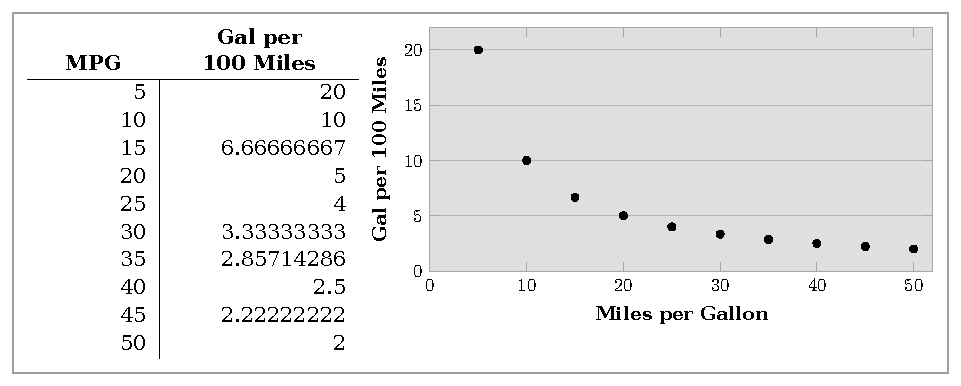
\includegraphics[width=.92\linewidth]{../figures/fhsm_2009_p24_f1.pdf}
\end{center}

The teacher then gives the class the article from the New York Times from which the quiz was taken to read for homework, along with some online comments from readers. She asks the students to analyze the arguments from the article in a brief essay and to propose what unit of measure they think will be useful for comparing the fuel consumption of cars.

One group made this report: ``The low mileage cars offer more opportunities for savings because they are using so much gas. If you go from $10$ MPG to $20$ MPG, you go from using $10$ gallons for $100$ miles to $5$ gallons. You have saved $5$ gallons per hundred miles, and that is as much as you are using after the improvement. If you double the rate again to $40$ MPG, you will still use 2½ gallons in 100 miles, so you have only saved 2½ gallons from the $20$ MPG amount or 7½ gallons from the $10$ MPG amount. Even if you double again, to $80$ MPG, you will still use $1.25$ gallons, so you have only saved an additional $1.25$ gallons from the $40$ MPG amount. The point seems to be, the less you use, the less savings you have available. You can't save more than you use.''

\noindent
\textbf{Key Elements of Mathematics}

Reasoning with Number and Measurement---Reasonableness of answers and
measurements 

Reasoning with Functions---Multiple representations of functions 

\noindent
\textbf{Reasoning Habits}

Analyzing a problem-seeking patterns and relationships

Reflecting on a solution---interpreting a solution; reconciling different approaches; refining arguments
}
{Ngẫm về nhiên liệu}
{
\noindent
\textbf{Nhiệm vụ}

Một giáo viên đưa cho học sinh Một giáo viên đưa cho học sinh bài trắc nghiệm sau đây, được trích từ một bài báo trên New York Times (Chang 2008), và yêu cầu các em giải thích lập luận của mình:

\textbf{Câu hỏi trắc nghiệm:} Trường hợp nào sau đây sẽ tiết kiệm được nhiều nhiên liệu hơn?

\begin{enumerate}
  \item [(a)] Thay một chiếc xe cỡ nhỏ đi được $34$ dặm trên mỗi ga-lông (MPG) bằng một chiếc xe lai đi được $54$ MPG.
  \item [(b)] Thay một chiếc thể thao đa dụng (SUV) đi được $18$ MPG bằng một chiếc xê-đan đi được $28$ MPG.
  \item [(c)] Cả hai sự thay đổi đều tiết kiệm được cùng một lượng nhiên liệu.
\end{enumerate}

\noindent
\textbf{Trong lớp học (Đại số năm thứ nhất)}

Giáo viên thu lại các bài làm và mời hai học sinh chia sẻ đáp án của mình với cả lớp. Học sinh thứ nhất trả lời:

\begin{quote}
  Em cho rằng đáp án đúng là (a). Lập luận của em là: mức thay đổi từ $34$ MPG lên $54$ MPG là tăng khoảng $59$ phần trăm, còn mức thay đổi từ $18$ MPG lên $28$ MPG chỉ tăng khoảng $56$ phần trăm.
\end{quote}

Học sinh thứ hai trả lời:

\begin{quote}
  Em nghĩ đến việc sẽ cần bao nhiêu xăng để đi một quãng đường $100$ dặm.

  \emph{Xét chiếc xe cỡ nhỏ:}

  $100$ dặm/$54$ MPG = $1.85$ ga-lông xăng đã dùng.

  $100$ dặm/$34$ MPG = $2.94$ ga-lông xăng đã dùng. 

  Vậy chuyển từ xe $34$ MPG sang xe $54$ MPG sẽ tiết kiệm được $1.09$ ga-lông xăng.

  \emph{Xét chiếc SUV:}

  $100$ dặm/$28$ MPG = $3.57$ ga-lông xăng đã dùng.

  $100$ dặm/$18$ MPG = $5.56$ ga-lông xăng đã dùng.

  Vậy chuyển từ xe $18$ MPG sang xe $28$ MPG sẽ tiết kiệm được $1.99$ ga-lông xăng trên mỗi $100$ dặm. Điều đó có nghĩa là trên thực tế, thay chiếc xe thể thao đa dụng sẽ tiết kiệm được nhiều xăng hơn.
\end{quote}

Sau đó, giáo viên yêu cầu cả lớp so sánh hai câu trả lời này. Sau một cuộc tranh luận sôi nổi giữa những học sinh đã chọn các đáp án khác nhau, cả lớp đi đến thống nhất rằng cả hai cách trả lời đều có điểm hợp lý, tùy theo cách hiểu bài toán. Mặc dù hiệu suất sử dụng nhiên liệu của chiếc xe cỡ nhỏ tăng nhiều hơn đôi chút, nhưng chủ xe trên thực tế sẽ tiết kiệm được nhiều ga-lông xăng hơn khi thay chiếc xe thể thao đa dụng, nếu cả hai xe đều đi cùng một số dặm như nhau.

Giáo viên yêu cầu cả lớp khảo sát mối quan hệ giữa MPG và lượng xăng thực tế tiêu thụ. Sau khi học sinh làm việc theo nhóm nhỏ trong vài phút, giáo viên mời một nhóm trình bày bảng giá trị và đồ thị mà nhóm đã lập, như ở dưới đây. Các em giải thích: ``Khi cứ tăng thêm $5$ MPG hết lần này đến lần khác, lượng nhiên liệu tiết kiệm được lại ít đi. Vì vậy, như chúng ta đã thấy trong câu hỏi trắc nghiệm, MPG có thể gây hơi khó hiểu.''

\begin{center}
  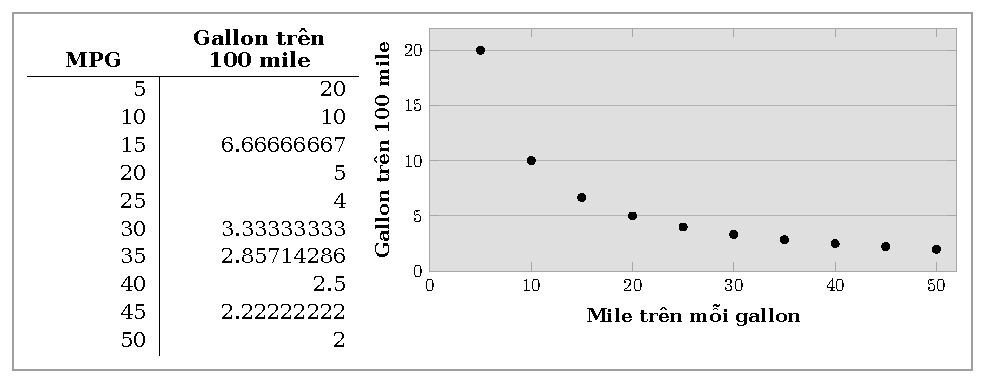
\includegraphics[width=.92\linewidth]{../figures/fhsm_2009_p24_f1_vi.pdf}
\end{center}

Sau đó, giáo viên giao cho cả lớp bài báo trên New York Times mà câu hỏi trắc nghiệm đã lấy từ đó để đọc ở nhà, cùng với một số bình luận trực tuyến của độc giả. Cô yêu cầu học sinh phân tích các lập luận trong bài báo bằng một bài viết ngắn và đề xuất đơn vị đo nào mà các em cho là hữu ích để so sánh mức tiêu thụ nhiên liệu của các xe.

Một nhóm đã viết báo cáo như sau: ``Những xe có mức đi được ít dặm trên mỗi ga-lông tạo ra nhiều cơ hội tiết kiệm hơn, vì chúng tiêu tốn quá nhiều xăng. Nếu bạn tăng từ $10$ MPG lên $20$ MPG, thì mức sử dụng sẽ giảm từ $10$ ga-lông cho mỗi $100$ dặm xuống còn $5$ ga-lông. Bạn đã tiết kiệm được $5$ ga-lông trên mỗi trăm dặm, và lượng đó đúng bằng mức bạn còn dùng sau khi cải thiện. Nếu lại tăng gấp đôi một lần nữa, lên $40$ MPG, thì bạn vẫn sẽ dùng $2½$ ga-lông trong $100$ dặm, nên bạn chỉ tiết kiệm thêm được $2½$ ga-lông so với mức $20$ MPG, hoặc tiết kiệm được $7½$ ga-lông so với mức $10$ MPG. Ngay cả khi lại tăng gấp đôi lần nữa, lên $80$ MPG, thì bạn vẫn sẽ dùng $1.25$ ga-lông, nên bạn chỉ tiết kiệm thêm được $1.25$ ga-lông so với mức $40$ MPG. Điểm chính dường như là: dùng càng ít thì phần còn có thể tiết kiệm được càng ít. Bạn không thể tiết kiệm nhiều hơn mức mình đang dùng.''

\noindent
\textbf{Các yếu tố toán học then chốt}

Luận với Số và Đo lường---Tính hợp lý của đáp số và phép đo.  

Luận với Hàm số---Nhiều biểu diễn của hàm số.

\noindent
\textbf{Thói quen lập luận}

Phân tích bài toán---tìm kiếm các mẫu hình và quan hệ  

Phản tư về lời giải---diễn giải lời giải; dung hòa các cách tiếp cận khác nhau; tinh chỉnh lập luận.
}
{
Ví dụ này cho thấy cùng một tình huống thực tế có thể dẫn đến hai cách trả lời khác nhau nếu ta chọn hai đại lượng so sánh khác nhau. Học sinh thứ nhất so sánh mức tăng của chỉ số MPG và kết luận rằng trường hợp (a) tốt hơn, vì $34$ lên $54$ MPG là một mức tăng phần trăm lớn hơn $18$ lên $28$ MPG. Tuy nhiên, học sinh thứ hai lại cố định quãng đường là $100$ dặm rồi tính lượng xăng thực sự tiêu thụ, nên thấy rằng thay chiếc xe thể thao đa dụng mới tiết kiệm được nhiều ga-lông xăng hơn. Điểm cốt lõi là MPG đo số dặm đi được trên một ga-lông, còn điều ta thật sự muốn biết ở đây là số ga-lông cần dùng cho cùng một quãng đường. Khi đổi sang đơn vị \emph{ga-lông trên $100$ dặm}, như bảng giá trị và đồ thị cho thấy, lượng xăng tiêu thụ giảm rất nhanh ở vùng MPG thấp rồi giảm chậm dần khi MPG tăng lên; vì thế, tăng thêm cùng một số MPG không tạo ra cùng một mức tiết kiệm nhiên liệu. Do đó, ví dụ này giúp học sinh nhận ra rằng muốn so sánh mức tiêu thụ nhiên liệu một cách có ý nghĩa, cần chọn đại lượng đo phù hợp với câu hỏi đang đặt ra, chứ không chỉ nhìn vào chỉ số MPG một cách trực tiếp.
}

\ParallelSection
  {Approximations and Error}
  {Xấp xỉ và sai số}
  {}

\TriPara
{
\EN{Pure mathematics is exact, but when we want to apply it to the world, we must learn to cope with approximation. Numbers obtained through measurement rather than counting are subject to error, an important concept with which students need to struggle (Lehrer 2003). ``Error'' does not mean ``mistake''; it is the unavoidable inexactness that is inherent in all real-world situations. Many high school students have not grasped the significance of reporting their measure to the nearest unit or subunit of measurement, depending on the measuring device. Moreover, the accuracy of the measurement affects any results that are subsequently reported. When scientists give results based on measurements---often a mixture of direct and computed measures---they are careful to report the method(s) used to obtain them. Students should realize that in a measurement, the digits beyond the first few are likely not relevant and that they should be suspicious when they see measurements with many decimal places in news reports. Students should learn that the accuracy of a result can be more effectively specified using the idea of \emph{relative error}. Relative error is illustrated in example 3, as is the need for students to monitor their progress and adjust their strategies accordingly.}
}
{
\VI{Toán học thuần túy là chính xác, nhưng khi muốn áp dụng toán vào thế giới thực, chúng ta buộc phải đối mặt với các dạng xấp xỉ. Những con số thu được thông qua đo đạc thay vì đếm trực tiếp luôn chịu ảnh hưởng của sai số, một khái niệm quan trọng mà học sinh cần phải vật lộn để hiểu (Lehrer, 2003). ``Sai số'' không có nghĩa là ``lỗi sai''; nó là sự không chính xác không thể tránh khỏi vốn có trong mọi tình huống thực tế. Nhiều học sinh trung học vẫn chưa hiểu được ý nghĩa của việc ghi lại số đo đến đơn vị gần nhất hoặc phần nhỏ của đơn vị, tùy thuộc vào dụng cụ đo. Hơn nữa, độ chính xác của phép đo ảnh hưởng đến mọi kết quả được tính toán dựa trên số đo đó. Khi các nhà khoa học công bố kết quả dựa trên phép đo---thường là sự kết hợp giữa giá trị đo trực tiếp và giá trị được tính toán---họ luôn cẩn thận ghi rõ phương pháp đo. Học sinh cần nhận ra rằng trong một phép đo, các chữ số vượt quá hai hoặc ba chữ số đầu tiên thường không còn mang ý nghĩa thực tế, và các em cần biết hoài nghi khi nhìn thấy các số đo có nhiều chữ số thập phân trong các bản tin. Học sinh cần học rằng độ chính xác của một kết quả có thể được mô tả hiệu quả hơn bằng \emph{sai số tương đối}. Khái niệm này được minh họa trong Ví dụ 3, đồng thời ví dụ đó cũng nhấn mạnh nhu cầu học sinh phải theo dõi tiến trình lập luận và điều chỉnh chiến lược khi cần thiết.}
}
{
\NOTE{}
}

\TriExample
{Around Pi}
{
\noindent
\textbf{Task}

Although we know that $\pi$ is an irrational number, we often use such approximations as $3.14$ or $22/7$. How much error are we introducing by using such an approximation? Find an upper bound for the relative error, and illustrate with a specific example.

\noindent
\textbf{In the Classroom (Second-Year Algebra)}

Helping students move beyond the notion of error as a mistake is an important part of the sense-making process for a productive discussion of error. Students may view error as \emph{how far they are from a correct answer}. The teacher can build on this view to discus \emph{error} as the difference between an approximation $(v)$ and the ``real'' value $(V)$, and \emph{absolute error} as the absolute value or magnitude of the error, $\lvert V - v\rvert$. Developing an understanding of \emph{relative error} as a percent of the ``real'' value can help students make sense of the formula for relative error, $\frac{\lvert V-v\rvert}{V}$. To better understand his students' progress in understanding relative error, a teacher assigns the ``Around Pi'' task as an in-class assessment to be completed individually. One student's response follows, with the teacher's comments in the margin:

\begin{quotation}
  I usually use $3.14$, so I decided to try that in the formula. But when I tried to figure out $\lvert V-v\rvert$, I got confused since we don't have an actual value for $V$ ($\pi$). But then I got this idea that I can be sure it is less than $.0016$, since $\pi<3.14159\dots$. So then I thought about $\frac{\lvert V-v\rvert}{V}$. We still don't know what $\pi$ is, but since $V$ is in the denominator, I'll pick something less than $V$, which would be $3.1416$. So $\frac{.0016}{3.1415}=9.0931\times 10^{-4}$. That's really small! Then I tried this with the area of a circle, with radius $5$, using $3.14$ and the $\pi$-button on my calculator, and it was only off by about $.0399$, so I guess that's pretty good!

  \emph{Great idea! But you could explain this a little more fully.}

  \emph{Why did you change to less? Why was that important? Is this the exact value? Continue your argument using bounds. Is this relative error? Have you really mabd your point with this example? How does using the $\pi$-button relate to the value of $V$?}
\end{quotation}

\noindent
\textbf{Key Elements of Mathematics}

Reasoning with Number and Measurement---Approximations and error


\noindent
\textbf{Reasoning Habits}

Analyzing a problem---defining relevant variables and conditions

Implementing a strategy---monitoring progress toward a solution

Reflecting on a solution---justifying or validating a solution; refining arguments
}
{Quanh số $\pi$}
{
\noindent
\textbf{Nhiệm vụ}

Mặc dù chúng ta biết rằng $\pi$ là một số vô tỉ, nhưng trong thực tế ta thường dùng các giá trị xấp xỉ như $3.14$ hoặc $22/7$. Khi dùng một giá trị xấp xỉ như vậy, ta đã tạo ra bao nhiêu sai số? Hãy tìm một cận trên cho sai số tương đối, và minh họa bằng một ví dụ cụ thể.

\noindent
\textbf{Trong lớp học (Đại số năm thứ hai)}

Việc giúp học sinh vượt qua quan niệm rằng sai số là một lỗi sai là một phần quan trọng của quá trình kiến tạo ý nghĩa, để có một thảo luận hiệu quả về sai số. Học sinh thường xem sai số như \emph{mức độ cách xa câu trả lời đúng}. Giáo viên có thể dựa trên quan niệm này để thảo luận về \emph{sai số} như hiệu giữa giá trị xấp xỉ $(v)$ và ``giá trị thật'' $(V)$, và \emph{sai số tuyệt đối} là giá trị tuyệt đối (độ lớn) của sai số, $\lvert V - v\rvert$. Việc hình thành hiểu biết về \emph{sai số tương đối} như là một tỉ lệ phần trăm của ``giá trị thật'' có thể giúp học sinh hiểu được công thức sai số tương đối, $\frac{\lvert V - v\rvert}{V}$. Để hiểu rõ hơn mức độ tiến bộ của học sinh trong việc nắm bắt khái niệm sai số tương đối, giáo viên giao nhiệm vụ ``Quanh số $\pi$'' như một bài đánh giá ngay trên lớp, yêu cầu học sinh làm cá nhân. Sau đây là lời giải của một học sinh, kèm theo nhận xét bên lề của giáo viên:

\begin{quote}
  Em thường dùng $3.14$, nên em quyết định thử dùng giá trị này trong công thức. Nhưng khi em cố tính $\lvert V - v\rvert$, em bị rối vì ta không có giá trị thật sự của $V$ (là $\pi$). Sau đó em nảy ra ý rằng ta có thể chắc chắn sai số tuyệt đối nhỏ hơn $0.0016$, vì $\pi < 3.14159\dots$. Vậy nên em xét $\frac{\lvert V - v\rvert}{V}$. Ta vẫn chưa biết chính xác $\pi$ là bao nhiêu, nhưng vì $V$ nằm ở mẫu số, em chọn một số nhỏ hơn $V$, đó là $3.1415$. Như vậy $0.0016 / 3.1415 \approx 9.0931 \times 10^{-4}$. Con số này rất nhỏ! Rồi em thử áp dụng vào diện tích hình tròn bán kính $5$, dùng $3.14$ và dùng nút $\pi$ trên máy tính, thì kết quả chênh lệch chỉ khoảng $0.0399$, nên em nghĩ như vậy là khá ổn!

  \textbf{Nhận xét của giáo viên}
  
  \emph{Ý tưởng rất hay! Nhưng em có thể giải thích đầy đủ hơn một chút.}

  \emph{Tại sao em lại chuyển sang dùng một giá trị nhỏ hơn? Điều đó quan trọng ở chỗ nào? Đây có phải là giá trị chính xác không? Hãy tiếp tục lập luận bằng cách dùng các cận trên/dưới. Đây có thực sự là sai số tương đối không? Ví dụ cuối cùng của em đã làm rõ được luận điểm của mình chưa? Việc dùng nút $\pi$ trên máy tính liên quan thế nào đến giá trị $V$?}
\end{quote}

\noindent
\textbf{Các yếu tố then chốt của toán học}

Luận với số và đo lường---Xấp xỉ và sai số

\noindent
\textbf{Các thói quen luận}

Phân tích bài toán---xác định cẩn thận các biến và điều kiện thích đáng

Triển khai chiến lược---theo dõi tiến trình đi đến lời giải  

Phản tư về lời giải---biện minh hoặc kiểm chứng một lời giải; tinh chỉnh lập luận
}
{
Ví dụ 3 cho thấy sai số không được đặt ra như một mẩu kiến thức phụ kèm theo đo lường, mà như một đối tượng của luận. Điều cần học không chỉ là tên gọi của sai số tuyệt đối và sai số tương đối, mà là cách dùng bất đẳng thức và các cận để kiểm soát độ lớn của sai số ngay cả khi giá trị đang xét không được biết chính xác dưới dạng thập phân hữu hạn. Điểm đáng chú ý ở đây là học sinh đã đi đúng hướng khi tìm cách chặn sai số, nhưng lại bộc lộ một lẫn lộn quan trọng trong cách viết và hiểu giá trị gần đúng của $\pi$. Sai sót ấy không làm hỏng giá trị của ví dụ; ngược lại, nó cho thấy hiểu trong toán không thể tách rời sự chính xác của ngôn ngữ và kí hiệu.

Các nhận xét của giáo viên cũng bộc lộ rõ lập trường sư phạm của sách. Giáo viên không sửa hộ lời giải, mà buộc học sinh nói rõ vì sao chọn một số nhỏ hơn hay lớn hơn giá trị cần xét, vì sao cách chọn ấy giúp ước lượng sai số, và ví dụ tính diện tích hình tròn ở cuối cùng thực sự chứng minh được điều gì. Trọng tâm vì thế không nằm ở việc chữa một lỗi riêng lẻ, mà ở việc đẩy học sinh đi tiếp từ trực giác ban đầu sang một lập luận chặt hơn.

Ví dụ này cũng làm sáng tỏ mối liên hệ giữa luận và hiểu. Khi so sánh kết quả dùng $\pi \approx 3.14$ với kết quả dùng một giá trị gần đúng tốt hơn của $\pi$, học sinh bắt đầu thấy sai số trong hằng số kéo theo sai khác ra sao trong đại lượng được tính. Nhờ đó, giá trị gần đúng không còn là một con số thay thế tùy tiện, mà được hiểu trong quan hệ với mục đích tính toán và mức chính xác cần có.

\textbf{Bài tập.} Hãy sử dụng bất đẳng thức $3.1415<\pi<3.1416$ để xây dựng thêm một lập luận.
}

\ParallelSection
  {Number Systems}
  {Các hệ thống số}
  {}

\TriPara
{
\EN{A solid understanding of number systems and their properties sets a foundation for meaningful development of algebra (Carraher and Schliemann 2007). Example 4 illustrates how an understanding of the distributive property with multidigit multiplication forms the basis for multiplication of polynomials; this point is further elaborated in example 6, ``Distribute Thoroughly''.}
}
{
\VI{Một sự hiểu biết vững chắc về các hệ thống số và các tính chất của chúng tạo nền tảng cho sự phát triển có ý nghĩa của đại số (Carraher và Schliemann, 2007). Ví dụ 4 minh họa cách hiểu về tính phân phối trong phép nhân nhiều chữ số tạo thành cơ sở cho phép nhân các đa thức; điểm này được trình bày chi tiết hơn trong Ví dụ 6, ``Phân phối triệt để''.}
}
{
\NOTE{}
}

\TriExample
{A Model Idea}
{
\noindent
\textbf{Background}

The distributive property can be illustrated with an *area model*. Take, for example, the product of 62 and 43. If each factor is written in expanded form, we have

$$
  \begin{aligned}
    (62)(43)
      &=(60+2)(40+3)\\
      &=24(100)+18(10)+8(10)+6.
  \end{aligned}
$$

The figure below shows groups of 100, 10, and 1 represented geometrically, helping students make sense not only of the distributive property but also of perfect squares and orders
of magnitude.

\begin{center}
  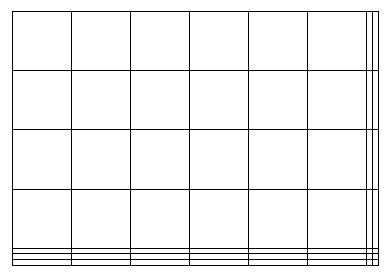
\includegraphics[width=.92\linewidth]{../figures/fhsm_2009_p27_1.pdf}
\end{center}

Once the concept of using area to model multiplication of integers has been established, ideally in kindergarten-grade 8, area models can help students make sense of many processes, such as multiplication of fractions and polynomials.

\noindent
\textbf{Task}

The distributive property for multiplication of variables can be modeled for such expressions as $A(B + C)$. As shown in the figure that follows, $AB + AC = A(B + C)$.

\begin{center}
  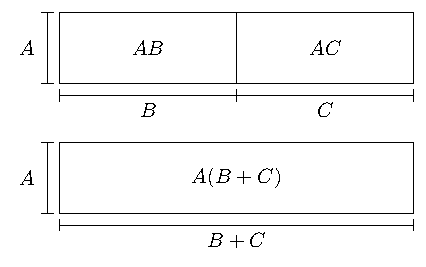
\includegraphics[width=.92\linewidth]{../figures/fhsm_2009_p28_1.pdf}
\end{center}

Create an area model for the product $(x + 3)(x + y + 5)$.

\noindent
\textbf{In the Classroom (First-Year Algebra)}

Students could create area models by drawing on graph paper or using algebra tiles. Two possible area models are shown below. The first shows regions of area $x^2$, $xy$, $x$, $y$, and $1$. By counting the number of each type of region present (i.e., one group of $x^2$ , three groups of $y$, and so forth), students can make sense of what each term in the expansion of the product represents. The second model shows the area of each smaller rectangular region as the product of its dimensions. This type of area model illustrates that the sum of the smaller areas (products of terms) is equal to the area of the original factors, thus forming a connection with the area addition postulate. 

\begin{center}
  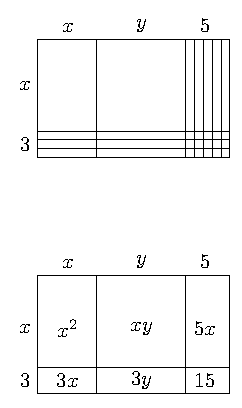
\includegraphics[width=.92\linewidth]{../figures/fhsm_2009_p28_2.pdf}
\end{center}

\textbf{Key Elements of Mathematics}

Reasoning with Number and Measurement---Number systems 

\textbf{Reasoning Habits}

Analyzing a problem---identifying relevant concepts, procedures, or representations; applying previously learned concepts 

Seeking and using connections
}
{Một ý tưởng mô hình}
{
\noindent
\textbf{Bối cảnh}

Tính phân phối có thể được minh họa bằng một \emph{mô hình diện tích}. Chẳng hạn, xét tích của $62$ và $43$. Nếu mỗi thừa số được viết dưới dạng khai triển, ta có

$$
  \begin{aligned}
    (62)(43)
      &=(60+2)(40+3)\\
      &=24(100)+18(10)+8(10)+6.
  \end{aligned}
$$

Hình bên dưới biểu diễn các nhóm $100$, $10$ và $1$ bằng hình học, giúp học sinh hiểu không chỉ tính phân phối mà cả các bình phương và các bậc độ lớn.

\begin{center}
  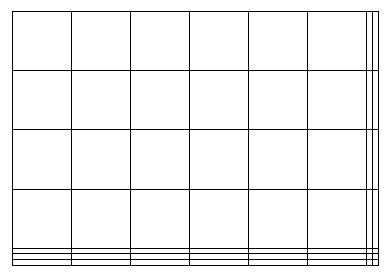
\includegraphics[width=.92\linewidth]{../figures/fhsm_2009_p27_1.pdf}
\end{center}

Khi ý tưởng dùng diện tích để mô hình hóa phép nhân số nguyên đã được hình thành (lý tưởng là từ bậc tiểu học đến trung học cơ sở), các mô hình diện tích có thể giúp học sinh hiểu nhiều quy trình khác, chẳng hạn như phép nhân phân số và phép nhân đa thức.

\noindent
\textbf{Nhiệm vụ}

Tính phân phối trong phép nhân các biểu thức chứa biến có thể được mô hình hóa cho những biểu thức như $A(B + C)$. Như minh họa trong hình sau, $AB + AC = A(B + C)$.

\begin{center}
  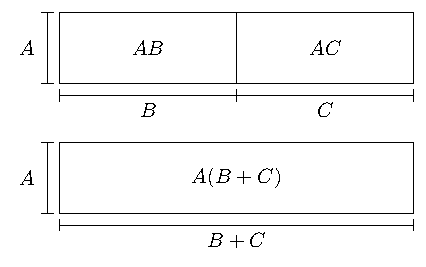
\includegraphics[width=.92\linewidth]{../figures/fhsm_2009_p28_1.pdf}
\end{center}

Hãy tạo một mô hình diện tích cho tích $(x + 3)(x + y + 5)$.

\noindent
\textbf{Trong lớp học (Đại số năm thứ nhất)}

Học sinh có thể tạo các mô hình diện tích bằng cách vẽ trên giấy kẻ ô hoặc sử dụng các mảnh ghép đại số. Hai mô hình diện tích có thể có được minh họa dưới đây.

Mô hình thứ nhất cho thấy các vùng có diện tích $x$, $xy$, $x$, $y$ và $1$. Bằng cách đếm số vùng của mỗi loại (ví dụ: một vùng $x^2$, ba vùng $y$, v.v.), học sinh có thể hiểu ý nghĩa của từng hạng tử trong khai triển của tích.

Mô hình thứ hai thể hiện diện tích của từng hình chữ nhật nhỏ bằng tích của các cạnh tương ứng. Kiểu mô hình diện tích này minh họa rằng tổng diện tích các vùng nhỏ (tích của các hạng tử) bằng diện tích của hình chữ nhật ban đầu, từ đó kết nối với tiên đề cộng diện tích.

\begin{center}
  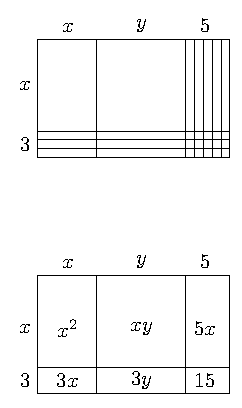
\includegraphics[width=.92\linewidth]{../figures/fhsm_2009_p28_2.pdf}
\end{center}

\noindent
\textbf{Các yếu tố then chốt của toán học}

Luận với số và đo lường---Các hệ thống số

\noindent
\textbf{Các thói quen luận}

Phân tích bài toán---xác định các khái niệm, thủ tục, hoặc biểu diễn toán học thích đáng; vận dụng các khái niệm đã học  

Tìm kiếm và sử dụng các kết nối
}
{}

\ParallelSection
  {Counting}
  {Đếm}
  {}

\TriPara
{
\EN{Counting principles and techniques, an important topic from discrete mathematics, have applications both within and outside mathematics. See example 20, ``What Are the Chances? Part A'' for an application of counting principles to probability models. Students need to understand the difference between counting the number of possible outcomes and enumerating all possible cases. For example, when rolling a pair of dice and summing the numbers of the topmost faces, eleven sums from $2$ to $12$ are possible. Yet not all sums are equally likely, because five ways exist to get $6$ ($1 + 5$, $2 + 4$, $3 + 3$, $4 + 2$, and $5 + 1$) but only one way to get $2$ $(1 + 1)$. Another important counting skill is understanding the difference between situations in which the order of events matters (e.g., the digits in a number) and situations in which order is irrelevant (e.g., membership on a committee, as in example 20, ``What Are the Chances? Part A'').}
}
{
\VI{Các nguyên lí và kĩ thuật đếm, một chủ đề quan trọng của toán rời rạc, có những ứng dụng cả trong toán lẫn ngoài toán. Xem Ví dụ 20, ``Bao nhiêu khả năng? Phần A'', để thấy một ứng dụng của các nguyên lí đếm vào các mô hình xác suất. Học sinh cần hiểu sự khác nhau giữa việc đếm số kết quả có thể có và việc liệt kê toàn bộ các trường hợp có thể xảy ra. Chẳng hạn, khi gieo một cặp xúc xắc rồi cộng số chấm ở hai mặt trên cùng, ta có thể thu được mười một tổng từ $2$ đến $12$. Tuy nhiên, không phải mọi tổng đều có khả năng xảy ra như nhau, vì có năm cách để được $6$ ($1 + 5$, $2 + 4$, $3 + 3$, $4 + 2$, và $5 + 1$), nhưng chỉ có một cách để được $2$ $(1 + 1)$. Một kĩ năng đếm quan trọng khác là hiểu sự khác nhau giữa những tình huống mà thứ tự của các sự kiện là quan trọng (chẳng hạn, các chữ số trong một số) và những tình huống mà thứ tự là không quan trọng (chẳng hạn, thành viên của một ủy ban, như trong Ví dụ 20, ``Bao nhiêu khả năng? Phần A'').}
}
{
\NOTE{}
}

\TriPara
{
\EN{A solid understanding of number and measurement continues to be important at the high school level because it provides the foundation for reasoning about other mathematical concepts. Helping students make sense of these essential ideas will ease their transition to more abstract topics.}
}
{
\VI{Hiểu biết vững chắc về số và đo lường vẫn tiếp tục giữ vai trò quan trọng ở bậc trung học phổ thông, vì nó cung cấp nền tảng cho việc luận về các khái niệm toán học khác. Việc giúp học sinh hiểu những ý niệm thiết yếu này sẽ làm cho quá trình chuyển sang các chủ đề trừu tượng hơn của các em trở nên thuận lợi hơn.}
}
{
\NOTE{}
}

% =========
% CHƯƠNG 5
% =========

\ParallelChapter
  {Reasoning with Algebraic Symbols}
  {Luận với ký hiệu đại số}
  {}

\TriPara
{
\EN{The algebraic notation we use today is a major accomplishment of humankind, allowing for the compact representation of complex calculations and problems (Fey 1984; Radford and Puig 2007). However, that very compactness can be a barrier to sense making (Radford and Puig 2007; Saul 2001). A basic task for teachers of algebra is to help students reason their way through that barrier.

Key elements of reasoning and sense making with algebraic symbols include the following:

\begin{itemize}
  \item \emph{Meaningful use of symbols.} Choosing variables and constructing expressions and equations in context; interpreting the form of expressions and equations; manipulating expressions so that interesting interpretations can be made.
  \item \emph{Mindful manipulation.} Connecting manipulation with the laws of arithmetic; anticipating the results of manipulations; choosing procedures purposefully in context; picturing calculations mentally.
  \item \emph{Reasoned solving.} Seeing solution steps as logical deductions about equality; interpreting solutions in context.
  \item \emph{Connecting algebra with geometry.} Representing geometric situations algebraically and algebraic situations geometrically; using connections in solving problems.
  \item \emph{Linking expressions and functions.} Using multiple algebraic representations to understand functions; working with function notation.
\end{itemize}

We address these key elements in more detail in the following sections.}
}
{
\VI{Ký hiệu đại số mà ta sử dụng ngày nay là một thành tựu lớn của nhân loại, cho phép biểu diễn gọn gàng những phép tính và bài toán phức tạp (Fey 1984; Radford và Puig 2007). Tuy nhiên, chính sự cô đọng đó đôi khi lại trở thành rào cản đối với việc hiểu (Radford và Puig 2007; Saul 2001). Một nhiệm vụ cơ bản của giáo viên đại số là giúp học sinh luận để vượt qua rào cản ấy.

Các yếu tố then chốt của luận và hiểu với các ký hiệu đại số gồm có:

\begin{itemize}
  \item \emph{Sử dụng ký hiệu có nghĩa.} Chọn biến và lập các biểu thức, phương trình trong ngữ cảnh; diễn giải dạng của các biểu thức và phương trình; biến đổi biểu thức để có thể đưa ra những diễn giải đáng chú ý.
  \item \emph{Biến đổi có ý thức.} Gắn việc biến đổi với các quy luật số học; dự đoán kết quả của các phép biến đổi; lựa chọn thủ tục có chủ đích trong ngữ cảnh; hình dung các phép tính trong đầu.
  \item \emph{Giải có luận cứ.} Nhìn nhận các bước giải như những suy diễn có tính luận lý về quan hệ bằng nhau; diễn giải nghiệm trong ngữ cảnh.
  \item \emph{Kết nối đại số với hình học.} Biểu diễn các tình huống hình học bằng đại số và các tình huống đại số bằng hình học; sử dụng các kết nối đó trong quá trình giải quyết vấn đề.
  \item \emph{Liên kết biểu thức và hàm số.} Sử dụng nhiều dạng biểu diễn đại số để hiểu biết hàm số; làm việc với ký hiệu hàm.
\end{itemize}

Chúng tôi sẽ trình bày chi tiết hơn các yếu tố then chốt này trong các phần tiếp theo.}
}
{
\NOTE{}
}

\ParallelSection
  {Meaningful Use of Symbols}
  {Sử dụng ký hiệu có nghĩa}
  {}

\TriPara
{
\EN{Meaningful use of symbols includes carefully defining the meaning of symbols introduced to solve problems, including specifying units and distinguishing among the three main uses of variables---(1) as unknowns (e.g., find the value of $Q$ such that $3Q - 4 = 11$), (2) as placeholders that can take on a range of values (e.g., $a + c = c + a$ for all $a$ and $c$), and (3) as parameters of a function (e.g., What is the effect of increasing m on the graph of $y = mx + b$?) (Usiskin 1988).}
}
{
\VI{Sử dụng ký hiệu có nghĩa bao gồm việc xác định rõ ràng ý nghĩa của các ký hiệu được đưa vào để giải quyết vấn đề, trong đó có việc chỉ rõ đơn vị đo và phân biệt ba cách sử dụng biến số: (1) như là ẩn số (ví dụ: tìm giá trị của $Q$ sao cho $3Q - 4 = 11$); (2) như là ký hiệu giữ chỗ có thể nhận nhiều giá trị (ví dụ: $a + c = c + a$ với mọi $a$ và $c$); (3) như là tham số của một hàm số (ví dụ: ảnh hưởng của việc tăng $m$ đối với đồ thị của hàm $y = mx + b$ là gì?) (Usiskin 1988).}
}
{
\NOTE{Có ba loại biến: 

\begin{itemize}
  \item biến-ẩn số,
  \item biến-tham số,
  \item biến-giữ chỗ (biến-tự do).
\end{itemize}
}
}

\TriPara
{
\EN{Although a long-term goal of algebraic learning is a fluid, nearly automatic facility with manipulating algebraic expressions that might seem to resemble what is often called ``mindless manipulation,'' this ease can best be achieved by first learning to pay close attention to interpreting expressions, both at a formal level and as statements about real-world situations. At the outset, the reasons and justifi cations for forming and manipulating expressions should be major emphases of instruction (Kaput, Blanton, and Moreno 2008). As comfort with expressions grows, constructing and interpreting them require less and less effort and gradually become almost subconscious. The true foundation for algebraic manipulation is close attention to meaning and structure.}
}
{
\VI{Mặc dù một mục tiêu dài hạn của việc học đại số là đạt tới sự thành thạo trôi chảy, gần như tự động, trong việc biến đổi các biểu thức đại số, một năng lực thoạt nhìn có thể giống với điều thường được gọi là ``sự biến đổi vô thức'', thì sự thành thạo ấy được hình thành tốt nhất khi trước hết người học học cách chú ý sát sao đến việc diễn giải các biểu thức, cả ở bình diện hình thức lẫn ở bình diện như những phát biểu về các tình huống trong thế giới thực. Ở giai đoạn đầu, các lí do và sự biện minh cho việc lập nên và biến đổi các biểu thức cần phải là những trọng tâm lớn của dạy học (Kaput, Blanton, and Moreno 2008). Khi mức độ thành thạo với các biểu thức tăng lên, việc tạo lập và diễn giải chúng đòi hỏi ngày càng ít công sức hơn và dần trở nên gần như dưới ngưỡng ý thức. Nền tảng thực sự của việc biến đổi đại số là sự chú ý sát sao đến ý nghĩa và cấu trúc.}
}
{
\NOTE{}
}


\TriPara
{
\EN{Reasoning with algebraic expressions depends on being able to read them in different ways, for example, seeing $3 - (4 - x)^2$ as 3 minus a quantity squared and thus as a value less than or equal to 3, as a function of $4 - x$, and as a function of $x$. In example 5 students are asked to interpret the purposes of different forms of the same expression.}
}
{
\VI{Luận với biểu thức đại số phụ thuộc vào khả năng đọc chúng theo nhiều cách khác nhau. Chẳng hạn, biểu thức $3 - (4 - x)^2$ có thể được hiểu là $3$ trừ đi bình phương của một đại lượng, từ đó suy ra giá trị của nó luôn nhỏ hơn hoặc bằng $3$; đồng thời có thể được xem như một hàm theo biến $4 - x$, và cũng là một hàm theo biến $x$. Trong Ví dụ 5, học sinh được yêu cầu diễn giải mục đích của các dạng khác nhau của cùng một biểu thức.}
}
{
\NOTE{}
}

\TriExample
{Horeshoes in Flight}
{
\noindent
\textbf{Task}

The height of a thrown horseshoe depends on the time that has elapsed since its release, as shown in the graph. Note that this graph is parabolic, but it may not be the same as the graph of the horseshoe's path. Its height (measured in feet) as a function of time (measured in seconds) from the instant of release is

$$
  1\frac{3}{16}+18t-16t^2.
$$

\begin{center}
  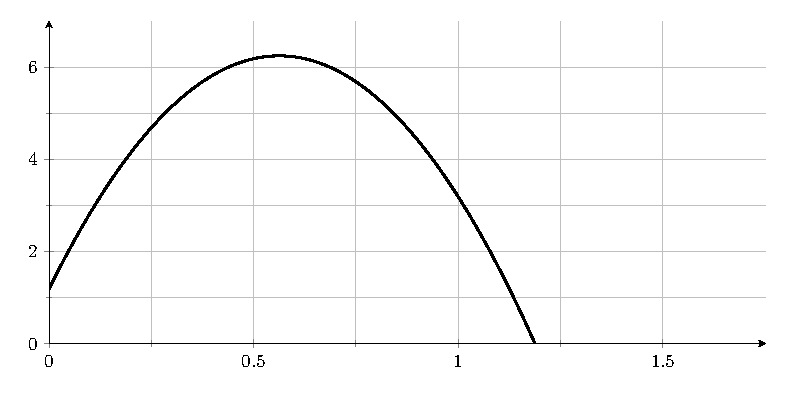
\includegraphics[width=.92\linewidth]{../figures/fhsm_2009_p32_1.pdf}
\end{center}

The expressions (a)--(d) below are equivalent. Which is most useful for finding the maximum height of the horseshoe, and why is it the most useful expression?

\begin{enumerate}
  \item [(a)] $1\frac{3}{16}+18-16t^2$
  \item [(b)] $-16\left(t-\frac{19}{16}\right)\left(t+\frac{1}{16}\right)$
  \item [(c)] $\frac{1}{16}\left(19-16t\right)\left(16t+1\right)$
  \item [(d)] $-16\left(t-\frac{19}{16}\right)^2+\frac{100}{16}$
\end{enumerate}

\noindent
\textbf{In the Classroom (Second-Year Algebra)}

\noindent
\emph{Group report:}

\begin{quote}
  We eliminated expression (a). It tells us the starting height and starting upward speed, but the question is not about either of those. Expressions (b) and (c) are pretty much the same, except that the denominators in the factors have been pulled out in front in (c). One of us used (b) to find the zeros ($\frac{19}{16}$ and $-\frac{1}{16}$), and then found the midpoint ($\frac{9}{16}$), which should be the time at which the maximum height is achieved. But we finally decided on (d) because the term

  $$
    -16\left(t-\frac{9}{16}\right)^2
  $$

  is always negative or zero, so we could see that the height never goes above $\frac{100}{16}$ feet, or $6\frac{1}{4}$ feet, and that it reaches this height at $t=\frac{9}{16}$ seconds, which is the same as the midpoint found by using (b).
\end{quote}

\noindent
\textbf{Key Elements of Mathematics}

Reasoning with Algebraic Symbols---Meaningful use of symbols; Linking expressions and functions

\noindent
\textbf{Reasoning Habits}

Analyzing a problem---looking for hidden structure

Reflecting on a solution---interpreting a solution; justifying or validating a solution
}
{Móng ngựa trên không}
{
\noindent
\textbf{Nhiệm vụ}

Độ cao của một chiếc móng ngựa được ném phụ thuộc vào thời gian đã trôi qua kể từ lúc nó rời tay, như được minh họa trên đồ thị. Lưu ý rằng đồ thị này có dạng parabol, nhưng không nhất thiết trùng với quỹ đạo chuyển động của móng ngựa. Độ cao của nó (tính bằng foot), như một hàm theo thời gian (tính bằng giây) kể từ thời điểm thả tay, được cho bởi

$$
1\frac{3}{16}+18t-16t^2.
$$

\begin{center}
  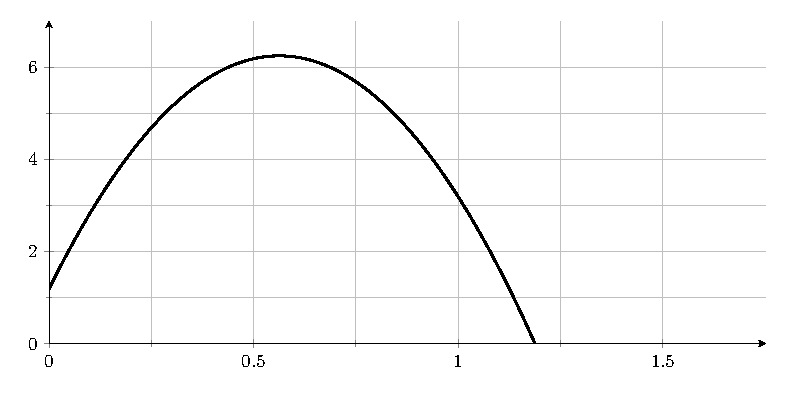
\includegraphics[width=.92\linewidth]{../figures/fhsm_2009_p32_1.pdf}
\end{center}

Các biểu thức (a)--(d) dưới đây là tương đương nhau. Biểu thức nào hữu ích nhất để tìm độ cao lớn nhất của móng ngựa, và vì sao đó là biểu thức hữu ích nhất?

\begin{enumerate}
  \item [(a)] $1\frac{3}{16}+18-16t^2$
  \item [(b)] $-16\left(t-\frac{19}{16}\right)\left(t+\frac{1}{16}\right)$
  \item [(c)] $\frac{1}{16}\left(19-16t\right)\left(16t+1\right)$
  \item [(d)] $-16\left(t-\frac{19}{16}\right)^2+\frac{100}{16}$
\end{enumerate}

\noindent
\textbf{Trong lớp học (Đại số năm thứ hai)}

\noindent
\emph{Báo cáo nhóm:}

\begin{quote}
  Chúng em loại biểu thức (a). Nó cho biết độ cao ban đầu và tốc độ đi lên ban đầu, nhưng câu hỏi không hỏi về điều nào trong hai điều đó. Các biểu thức (b) và (c) hầu như giống nhau, chỉ khác là ở (c), các mẫu số trong các thừa số đã được đưa ra ngoài phía trước. Một bạn trong nhóm dùng (b) để tìm các nghiệm $\left(\frac{19}{16} \text{ và } -\frac{1}{16}\right)$, rồi tìm trung điểm $\left(\frac{9}{16}\right)$, và đó phải là thời điểm mà độ cao cực đại đạt được. Nhưng cuối cùng chúng em chọn (d), vì hạng tử

  $$
    -16\left(t-\frac{9}{16}\right)^2
  $$

  luôn âm hoặc bằng không, nên chúng em thấy rằng độ cao không bao giờ vượt quá $\frac{100}{16}$ feet, hay $6\frac{1}{4}$ feet, và đạt tới độ cao này tại $t=\frac{9}{16}$ giây, đúng bằng trung điểm tìm được khi dùng (b).

\end{quote}

\noindent
\textbf{Các yếu tố then chốt của toán học}

Luận với ký hiệu đại số---Sử dụng kí hiệu có nghĩa; Liên kết biểu thức và hàm số

\noindent
\textbf{Các thói quen luận}

Phân tích bài toán---tìm kiếm cấu trúc ẩn

Phản tư về lời giải---diễn giải lời giải; biện minh hoặc kiểm chứng một lời giải
}
{}

\TriPara
{
\EN{Example 5 also raises a common difficulty to which teachers may need to be sensitive---confusion between a representation of the actual flight of an object (in this instance a horseshoe) and the time-versus-height graph. To help clarify this issue, teachers might ask such questions as ``How far do you think the horseshoe would travel?'' (certainly more than 1.2 feet) or “How do the scales of the two axes compare?”}
}
{
\VI{Ví dụ 5 cũng làm nổi bật một khó khăn phổ biến mà giáo viên cần lưu ý: sự nhầm lẫn giữa hình ảnh biểu diễn quỹ đạo chuyển động thực tế của một vật (trong trường hợp này là chiếc móng ngựa) và đồ thị biểu diễn mối quan hệ giữa thời gian và độ cao. Để làm rõ vấn đề này, giáo viên có thể đặt ra những câu hỏi như: ``Theo em, chiếc móng ngựa sẽ bay được bao xa?'' (chắc chắn là nhiều hơn 1.2 foot) hoặc ``Thang đo trên hai trục của đồ thị khác nhau như thế nào?''}
}
{
\NOTE{}
}

\ParallelSection
  {Mindful Manipulation}
  {Biến đổi có ý thức}
  {}

\TriPara
{
\EN{Mindful manipulation includes learning algebraic manipulation as a process guided by understanding and goals (how do I want to use this expression, and what will make it most useful for this purpose?) and seeing that the basic rules of arithmetic provide a rationale for all legitimate manipulations of polynomial expressions. Of these, the distributive property, which is the only rule connecting the operations of addition and multiplication, is the one to which we must constantly appeal when doing anything that involves both operations at once, including a wide range of manipulations: expanding, factoring, collecting like terms, and putting fractions over a common denominator. Example 6 illustrates the difference between mindless and mindful manipulation when multiplying polynomials. It also illustrates the importance of organizing one's solution.}
}
{
\VI{Biến đổi có ý thức bao gồm việc học các phép biến đổi đại số như một quá trình được dẫn dắt bởi sự hiểu biết và mục tiêu (ta muốn sử dụng biểu thức này để làm gì, và dạng nào sẽ khiến nó hữu ích nhất cho mục đích đó?), đồng thời nhận ra rằng các quy tắc cơ bản của số học chính là cơ sở lý giải cho mọi phép biến đổi hợp lệ của các biểu thức đa thức. Trong số các quy tắc này, tính chất phân phối, vốn là quy tắc duy nhất nối kết hai phép toán cộng và nhân, là quy tắc mà ta phải liên tục viện đến khi thực hiện bất kỳ thao tác nào có liên quan đồng thời đến cả hai phép toán, bao gồm một loạt các phép biến đổi như: khai triển, phân tích thành nhân tử, thu gọn các hạng tử đồng dạng, và quy đồng mẫu số. Ví dụ 6 minh họa sự khác biệt giữa biến đổi máy móc và biến đổi có ý thức khi nhân các đa thức. Đồng thời, ví dụ này cũng cho thấy tầm quan trọng của việc tổ chức lời giải.}
}
{
\NOTE{}
}

\TriExample
{
Distribute Thoroughly
}
{
\noindent
\textbf{Task}

Expand:

\begin{enumerate}
  \item [(a)] $(1 + x^3)(1 + x + x^2)$
  \item [(b)] $(1 + x)(1 + x + x^2)$
\end{enumerate}

\noindent
\textbf{In the Classroom (First-Year Algebra)}

Student 1 is accustomed to using the mnemonic FOIL (First, Outer, Inner, Last) to expand products of two binomials, such as $(1 + x)(1 + x^2)$, and applies it to the problem $(1 + x^3)(1 + x + x^2)$, getting $1 + x^2 + x^3 + x^5$ .

Student 2 says, ``You missed the products of the middle term, x, in the second factor. The distributive property means we have to multiply each term of one factor with each term of the other, and then add all the products.

So I get

$$
\begin{aligned}
  &(1 + x^3)(1 + x + x^2) \\ 
    &\quad= 1 \cdot 1 + 1 \cdot x + 1 \cdot x^2 + x^3 \cdot 1\\
    &\qquad + x^3 \cdot x + x^3 \cdot x^2 \\
    &\quad= 1 + x + x^2 + x^3 + x4 + x^5.
\end{aligned}
$$

I sometimes remember this as `each with each.' Sometimes you can just multiply the terms mentally. I like to visualize the steps and write as little as possible. For example, when I apply `each with each' to

$$
\begin{aligned}
  &(1 - x)(1 + x + x^2) \\
  &\quad = 1 + x + x^2 - x - x^2 - x^3 \\
  &\quad = 1 - x^3,
\end{aligned}
$$

I can see that the second and third terms from the multiplication by $1$ are opposites of the first and second terms from multiplication by $-x$, so I can just write down the remaining terms.''

\noindent
\textbf{Key Elements of Mathematics}

Reasoning with Algebraic Symbols---Meaningful use of symbols; Mindful manipulation

Reasoning with Numbers and Measurements-Number systems

\noindent
\textbf{Reasoning Habits}

Analyzing a problem---applying previously learned concepts

Implementing a strategy---making purposeful use of procedures; organizing the solution

Seeking and using connections
}
{Phân phối triệt để}
{
\noindent
\textbf{Nhiệm vụ}

Khai triển: 

\begin{enumerate}
  \item [(a)] $(1 + x^3)(1 + x + x^2)$
  \item [(b)] $(1 + x)(1 + x + x^2)$
\end{enumerate}

\noindent
\textbf{Trong lớp học (Đại số năm thứ nhất)}

Học sinh 1 đã quen dùng mẹo nhớ FOIL (First, Outer, Inner, Last) để khai triển tích của hai nhị thức, chẳng hạn như $(1 + x)(1 + x^2)$, và áp dụng nó vào bài toán $(1 + x^3)(1 + x + x^2)$, thu được $1 + x^2 + x^3 + x^5$.

Học sinh 2 nói: ``Bạn đã bỏ sót các tích có chứa hạng tử ở giữa, $x$, trong thừa số thứ hai. Tính phân phối có nghĩa là ta phải nhân mỗi hạng tử của một thừa số với mỗi hạng tử của thừa số kia, rồi cộng tất cả các tích lại.

Vì thế mình được

$$
\begin{aligned}
  &(1 + x^3)(1 + x + x^2) \\
    &\quad= 1 \cdot 1 + 1 \cdot x + 1 \cdot x^2 + x^3 \cdot 1 \\
    &\qquad + x^3 \cdot x + x^3 \cdot x^2 \\
    &\quad= 1 + x + x^2 + x^3 + x^4 + x^5.
\end{aligned}
$$

Đôi khi mình nhớ điều này bằng câu `mỗi với mỗi.' Đôi khi ta có thể nhân các hạng tử ngay trong đầu. Mình thích hình dung các bước và viết ít nhất có thể. Chẳng hạn, khi mình áp dụng `mỗi với mỗi' vào

$$
\begin{aligned}
  &(1 - x)(1 + x + x^2) \\
  &\quad = 1 + x + x^2 - x - x^2 - x^3 \\
  &\quad = 1 - x^3,
\end{aligned}
$$

mình có thể thấy rằng hạng tử thứ hai và thứ ba do phép nhân với $1$ tạo ra đối nhau với hạng tử thứ nhất và thứ hai do phép nhân với $-x$ tạo ra, nên mình chỉ cần viết ra các hạng tử còn lại.''


\noindent
\textbf{Các yếu tố then chốt của toán học}

Luận với kí hiệu đại số---Sử dụng kí hiệu có nghĩa; Biến đổi có ý thức

Luận với số và đo lường---Các hệ thống số

\noindent
\textbf{Các thói quen luận}

Phân tích bài toán---vận dụng các khái niệm đã học 

Triển khai chiến lược---vận dụng có chủ đích các thủ tục; tổ chức lời giải

Tìm kiếm và sử dụng các kết nối
}
{}

\ParallelSection
  {Reasoned Solving}
  {Giải có luận cứ}
  {}

\TriPara
{
\EN{Equation solving is a goal-oriented process of logical argument; it is based on general principles of equality and procedures of algebraic manipulation consistent with the rules of arithmetic. Problem solving with equations should include careful attention to increasingly difficult problems that span the border between arithmetic and algebra. Such problems can help students view algebra as a sense-making activity that extends one's problem-solving skills into domains in which reasoning as done in arithmetic becomes too complicated or cumbersome to carry out. Seeing the essential parallels between algebraic and arithmetic solution methods can help students realize that algebra is not something totally new but simply a more powerful tool for dealing with problems that are hard to approach with arithmetic by itself (Saul 2001). In example 7 we illustrate reasoned solving of equations. Worth noting is the fact that although one student used a standard algebraic approach and the other used reasoning based on the concrete context, the steps in their solutions are essentially the same. Examples of this sort can help students see algebra as an extension of concrete arithmetic reasoning.}
}
{
\VI{Việc giải phương trình là một quá trình lập luận có tính luận lý; nó dựa trên những nguyên lí chung của sự bằng nhau và những thủ tục biến đổi đại số phù hợp với các quy tắc số học. Việc giải quyết vấn đề bằng phương trình cần bao gồm sự chú ý cẩn trọng đến những bài toán ngày càng khó hơn, nằm ở vùng ranh giới giữa số học và đại số. Những bài toán như vậy có thể giúp học sinh nhìn đại số như một hoạt động kiến tạo hiểu, mở rộng năng lực giải quyết vấn đề của mình sang những miền mà cách lập luận theo lối số học trở nên quá phức tạp hoặc quá cồng kềnh để thực hiện. Việc nhìn ra những tương đồng cốt yếu giữa các phương pháp giải bằng đại số và bằng số học có thể giúp học sinh nhận ra rằng đại số không phải là một cái gì hoàn toàn mới, mà chỉ là một công cụ mạnh hơn để xử lí những bài toán khó tiếp cận nếu chỉ dùng riêng số học (Saul 2001). Trong Ví dụ 7, chúng tôi minh họa việc giải có luận cứ đối với phương trình. Điều đáng lưu ý là mặc dù một học sinh dùng cách tiếp cận đại số quen thuộc còn học sinh kia dùng lối lập luận dựa trên ngữ cảnh cụ thể, các bước trong hai lời giải ấy về thực chất là giống nhau. Những ví dụ kiểu này có thể giúp học sinh nhìn đại số như một sự mở rộng của lập luận số học cụ thể.}
}
{
\NOTE{}
}

\TriExample
{Finding Balance}
{
\noindent
\textbf{Task}

A slab of soap on one pan of a scale balances $\frac{3}{4}$ of a slab of soap of equal weight and a $\frac{3}{4}$-pound weight on the other pan. How much does the slab of soap weigh? Solve the problem both with an algebraic equation and by direct arithmetic reasoning.  (Adapted from Kordemsky and Parry [1992])

\noindent
\textbf{In the Classroom (Ninth-Grade Students' Solutions)}

\begin{scriptlist}
  \item [Student 1:] If $x$ is the weight of the slab in pounds, then one side of the balance weighs $x$ pounds and the other weighs

  $$
  \frac{3}{4}x+\frac{3}{4},
  $$

  so

  $$
  x=\frac{3}{4}x+\frac{3}{4}.
  $$

  Subtracting $\frac{3}{4}$ from both sides gives

  $$
  \frac{1}{4}x=\frac{3}{4}
  $$

  so $x=3$.

  \item [Student 2:] It's just as easy without equations! If a slab of soap balances $\frac{3}{4}$ of a slab and $\frac{3}{4}$ pound, take $\frac{3}{4}$ of a slab off each side. That leaves $\frac{1}{4}$ of a slab on one side and $\frac{3}{4}$ pound on the other. So a quarter of a slab weighs $\frac{3}{4}$ of a pound. A full slab is four quarters, and that will make $3$ pounds.
  \item [Teacher:] Good! Can you see the connection between your two solutions?
  \item [Student 1:] Oh, I see. What she did is really the same except she didn't use an $x$.
\end{scriptlist}

\noindent
\textbf{Key Mathematical Elements}

Reasoning with Algebraic Symbols---Meaningful use of symbols; Reasoned solving

\noindent
\textbf{Reasoning Habits}

Implementing a strategy---making purposeful use of procedures; making logical deductions Seeking and using connections
}
{Tìm thế cân bằng}
{
\noindent
\textbf{Nhiệm vụ}

Một bánh xà phòng đặt trên một đĩa cân thì cân bằng với $\frac{3}{4}$ bánh xà phòng cùng khối lượng và một quả cân $\frac{3}{4}$ pound đặt trên đĩa bên kia. Bánh xà phòng nặng bao nhiêu? Hãy giải bài toán bằng cả một phương trình đại số lẫn lập luận số học trực tiếp. (Phỏng theo Kordemsky and Parry [1992])

\noindent
\textbf{Trong lớp học (Lời giải của học sinh lớp Chín)}

\begin{scriptlist}
  \item [Học sinh 1:] Nếu gọi $x$ là khối lượng của bánh xà phòng, tính theo pound, thì một bên cân nặng $x$ pound, còn bên kia nặng

  $$
  \frac{3}{4}x+\frac{3}{4},
  $$

  nên

  $$
  x=\frac{3}{4}x+\frac{3}{4}.
  $$

  Trừ $\frac{3}{4}x$ ở cả hai vế, ta được

  $$
  \frac{1}{4}x=\frac{3}{4}
  $$

  nên $x=3$.

  \item [Học sinh 2:] Không cần phương trình cũng dễ như vậy thôi! Nếu một bánh xà phòng cân bằng với $\frac{3}{4}$ bánh xà phòng và $\frac{3}{4}$ pound, thì hãy lấy $\frac{3}{4}$ bánh xà phòng ra khỏi mỗi bên. Khi đó còn lại $\frac{1}{4}$ bánh xà phòng ở một bên và $\frac{3}{4}$ pound ở bên kia. Vậy một phần tư bánh xà phòng nặng $\frac{3}{4}$ pound. Một bánh đầy đủ gồm bốn phần tư, nên sẽ nặng $3$ pound.
  \item [Giáo viên:] Tốt! Em có nhìn ra mối liên hệ giữa hai lời giải của mình không?
  \item [Học sinh 1:] À, em hiểu rồi. Cách bạn ấy làm thực ra cũng y hệt, chỉ là bạn ấy không dùng $x$.
\end{scriptlist}

\noindent
\textbf{Các yếu tố then chốt của toán học}

Luận với kí hiệu đại số---Sử dụng kí hiệu có nghĩa; Giải có luận cứ

\noindent
\textbf{Các thói quen luận}

Triển khai chiến lược---vận dụng có chủ đích các thủ tục; thực hiện những suy diễn có tính luận lý

Tìm kiếm và sử dụng các kết nối
}
{}

\ParallelSection
  {Connecting Algebra with Geometry}
  {Kết nối đại số với hình học}
  {}

\TriPara
{
\EN{An interplay exists between algebra and geometry: such geometric representations as graphs or figures can cast light on algebraic expressions and equations, and algebraic representations can be used to deduce geometric relationships (Katz 2007). Example 8 shows how the area model given in example 4, ``A Model Idea,'' can be extended in a geometrically compelling way to help students make sense of completing the square, a process that students often find mysterious. This example additionally illustrates the power of an effective representation as a basis for reasoning and shows how structure can be uncovered in that representation to move toward a general solution.}
}
{
\VI{Giữa đại số và hình học có một sự tác động qua lại: những biểu diễn hình học như đồ thị hay hình vẽ có thể soi sáng các biểu thức và phương trình đại số, còn những biểu diễn đại số có thể được dùng để suy ra các quan hệ hình học (Katz 2007). Ví dụ 8 cho thấy cách mô hình diện tích được nêu trong Ví dụ 4, ``Một ý tưởng mô hình,'' có thể được mở rộng theo một cách có sức thuyết phục về mặt hình học để giúp học sinh hiểu phép hoàn thành bình phương, một quá trình mà học sinh thường thấy khó nắm bắt. Ví dụ này đồng thời cũng minh họa sức mạnh của một biểu diễn hiệu quả như một nền tảng cho luận, và cho thấy cách cấu trúc có thể được phát hiện ngay trong biểu diễn ấy để tiến tới một lời giải tổng quát.}
}
{
\NOTE{}
}

\TriExample
{Squaring It Away}
{
\noindent
\textbf{Task}

Find a way of solving the equation $x^2 + 10x = 144$ by using an area model.

\noindent
\textbf{In the Classroom (Intermediate Algebra Class)}

\begin{scriptlist}
  \item [Teacher:] Can anybody see how to think of $x^2 + 10x$ as an area?
  \item [Student 1:] Well, $x^2$ is the area of a square with side $x$, and $10x$ is the area of a rectangle with sides $x$ and $10$, so we can put the rectangle and the square together like this. [See the figure at the right.] But I don't see how this helps.
  
  \begin{center}
  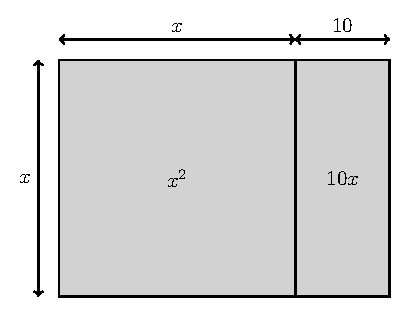
\includegraphics[width=.92\linewidth]{../figures/fhsm_2009_p36_1.pdf}
  \end{center}

  \item [Student 2:] Maybe if we knew what the area of the square was, we could just take the square root to find $x$.
  \item [Teacher:] Is there a way of rearranging the figure so that it's close to being a square?
  \item [Student 1:] I know! If we cut the rectangle into two rectangles of width $5$, we could put one on each side like this! [See the figure at the right.]
  
  \begin{center}
  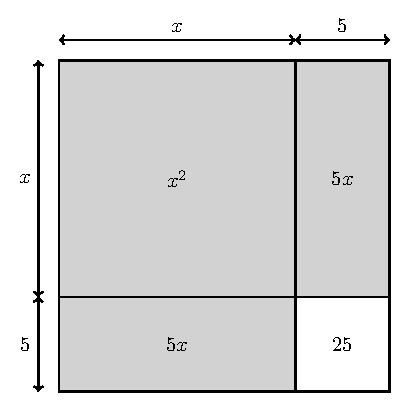
\includegraphics[width=.92\linewidth]{../figures/fhsm_2009_p36_2.pdf}
  \end{center}2

  \item [Student 2:] But it's not a complete square, it's missing a corner.
  \item [Teacher:] What's the area of the corner?
  \item [Student 2:] Oh, it must be $25$, since the white square lines up with ends of the rectangles, so it has side length $5$. And since the gray area is $144$, the entire area of the big square is $144 + 25 = 169$.
  \item [Student 1:] And that means the side length of the square is $13$, so $x + 5 = 13$, which means $x = 8$.
  \item [Student 2:] Shouldn't there be another solution, since the $(x + 5)$ is squared?
  \item [Teacher:] Interesting point. Let's take a closer look. Can you write down what you did algebraically?
  \item [Student 2:] We started with $x^2 + 10x = 144$, and then we added $25$ to the $144$. I guess that means we add $25$ to both sides of the equation, so we get $x^2 + 10x + 25 = 169$.
  \item [Student 1:] So to get $25$, we divide the $10$ by $2$ to get $5$, then square that to get $25$.
  \item [Student 2:] Yeah, and then the left-hand side is a perfect square, so you get $(x + 5)^2 = 169$.
  \item [Student 1:] The algebraic way gives you both solutions, because you get $x + 5 = 13$ or $x + 5 = -13$, so $x = 8$ or $x = -18$, but I guess the area model can't give you the negative solution.
  \item [Teacher:] Good observations. The process of adding a constant to a quadratic expression so that it becomes a perfect square is called ``completing the square.'' In the geometric interpretation, you just found that constant by adding in a corner piece. Can you see how this process might work for other quadratic equations?
\end{scriptlist}

The teacher could continue this discussion to lead to the development of the quadratic formula.

\noindent
\textbf{Key Mathematical Elements}

Reasoning with Algebraic Symbols---Meaningful use of symbols; Mindful manipulation;

Connecting algebra with geometry

\noindent
\textbf{Reasoning Habits}

Analyzing a problem---looking for hidden structure

Seeking and using connections

Reflecting on a solution---revisiting initial assumptions; generalizing a solution
}
{
Ổn thỏa bình phương
}
{
\noindent
\textbf{Nhiệm vụ}

Hãy tìm một cách giải phương trình $x^2 + 10x = 144$ bằng cách sử dụng mô hình diện tích.

\noindent
\textbf{Trong lớp học (Lớp Đại số trung cấp)}

\begin{scriptlist}
  \item [Giáo viên:] Có bạn nào thấy có thể nghĩ $x^2 + 10x$ như một diện tích không?
  \item [Học sinh 1:] Ừm, $x^2$ là diện tích của một hình vuông có cạnh dài $x$, còn $10x$ là diện tích của một hình chữ nhật có các cạnh $x$ và $10$, nên ta có thể ghép hình chữ nhật và hình vuông lại với nhau như thế này. [Xem hình bên phải.] Nhưng mình chưa thấy điều này giúp gì.
  
  \begin{center}
  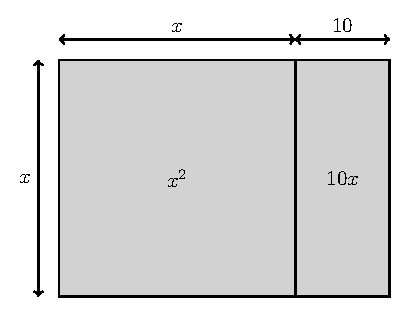
\includegraphics[width=.92\linewidth]{../figures/fhsm_2009_p36_1.pdf}
  \end{center}

  \item [Học sinh 2:] Có lẽ nếu biết diện tích của hình vuông là bao nhiêu thì ta chỉ việc lấy căn bậc hai để tìm $x$.
  \item [Giáo viên:] Có cách nào sắp xếp lại hình để nó gần thành một hình vuông không?
  \item [Học sinh 1:] Em biết rồi! Nếu cắt hình chữ nhật thành hai hình chữ nhật có chiều rộng $5$, ta có thể đặt một hình vào mỗi bên như thế này! [Xem hình bên phải.]
  
  \begin{center}
  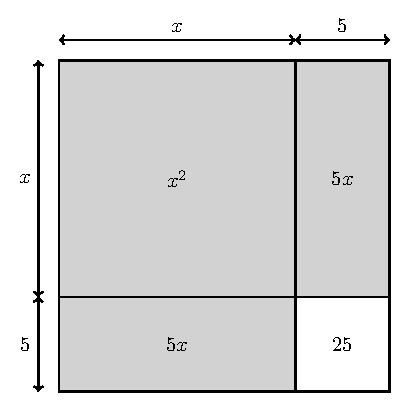
\includegraphics[width=.92\linewidth]{../figures/fhsm_2009_p36_2.pdf}
  \end{center}

  \item [Học sinh 2:] Nhưng nó chưa phải là một hình vuông hoàn chỉnh, nó còn thiếu một góc.
  \item [Giáo viên:] Diện tích của phần góc ấy là bao nhiêu?
  \item [Học sinh 2:] À, chắc phải là $25$, vì hình vuông trắng khớp với các đầu mút của các hình chữ nhật, nên nó có cạnh dài $5$. Và vì phần tô xám có diện tích là $144$, nên toàn bộ diện tích của hình vuông lớn là $144 + 25 = 169$.
  \item [Học sinh 1:] Và điều đó có nghĩa là cạnh của hình vuông là $13$, nên $x + 5 = 13$, suy ra $x = 8$.
  \item [Học sinh 2:] Chẳng phải phải có thêm một nghiệm nữa sao, vì $(x + 5)$ được bình phương?
  \item [Giáo viên:] Nhận xét thú vị đấy. Ta hãy xem kĩ hơn. Em có thể viết lại bằng đại số điều em vừa làm không?
  \item [Học sinh 2:] Chúng em bắt đầu với $x^2 + 10x = 144$, rồi cộng $25$ vào $144$. Chắc điều đó có nghĩa là phải cộng $25$ vào cả hai vế của phương trình, nên ta được $x^2 + 10x + 25 = 169$.
  \item [Học sinh 1:] Vậy để được $25$, ta lấy $10$ chia cho $2$ được $5$, rồi bình phương lên được $25$.
  \item [Học sinh 2:] Đúng, và khi đó vế trái là một bình phương hoàn chỉnh, nên ta được $(x + 5)^2 = 169$.
  \item [Học sinh 1:] Cách làm bằng đại số cho cả hai nghiệm, vì ta có $x + 5 = 13$ hoặc $x + 5 = -13$, nên $x = 8$ hoặc $x = -18$, nhưng em đoán là mô hình diện tích không cho được nghiệm âm.
  \item [Giáo viên:] Những nhận xét rất tốt. Quá trình cộng một hằng số vào một biểu thức bậc hai để nó trở thành một bình phương hoàn chỉnh được gọi là ``hoàn thành bình phương.'' Trong cách hiểu hình học, các em vừa tìm ra hằng số ấy bằng cách thêm vào một mảnh ở góc. Các em có thấy quá trình này có thể áp dụng thế nào cho những phương trình bậc hai khác không?
\end{scriptlist}

Giáo viên có thể tiếp tục cuộc thảo luận này để dẫn tới việc hình thành công thức nghiệm của phương trình bậc hai.

\noindent
\textbf{Các yếu tố then chốt của toán học}

Luận với kí hiệu đại số---Sử dụng kí hiệu có nghĩa; Biến đổi có ý thức; Kết nối đại số với hình học

\noindent
\textbf{Các thói quen luận}

Phân tích bài toán---tìm kiếm cấu trúc ẩn

Tìm kiếm và sử dụng các kết nối

Phản tư về lời giải---xem lại các giả định ban đầu; khái quát hóa lời giải
}
{
Ví dụ 8 đặc biệt đáng chú ý ở chỗ nó cho thấy hoàn thành bình phương có thể được dạy như một sự hướng tới một \emph{cấu trúc đích}, chứ không như một thủ thuật phải ghi nhớ. Điểm tựa của việc tổ chức dạy học ở đây là làm cho học sinh nhận ra rằng dạng

$$
(\text{bình phương}) = (\text{hằng số})
$$

là một dạng quen thuộc, dễ xử lí, vì khi ấy có thể giải bằng cách khai căn và xét các khả năng tương ứng. Từ điểm tựa ấy, phương trình
$$
x^2+10x=144
$$
được đọc không phải như một biểu thức cần biến đổi máy móc, mà như một biểu thức \emph{chưa đạt tới} cấu trúc mong muốn.

Theo hướng đó, hằng số $25$ không nên xuất hiện như một mẹo, mà như một tất yếu của cấu trúc: muốn vế trái trở thành một bình phương hoàn chỉnh thì phải có
$$
x^2+10x+25=(x+5)^2.
$$
Vai trò của mô hình diện tích là làm lộ ra và biện minh cho sự xuất hiện của phần bù ấy. Nó giúp học sinh \emph{thấy vì sao} cần thêm một mảnh góc có diện tích $25$, chứ không thay thế cho luận đại số. Chính ở điểm này, ví dụ cho thấy một biểu diễn hình học hiệu quả có thể nâng đỡ hiểu mà không làm mất đi bản chất của việc giải có luận cứ.

Cũng vì thế, giá trị sư phạm của ví dụ không nằm riêng ở việc tìm được nghiệm, mà ở việc làm sáng tỏ quan hệ giữa ba tầng: cấu trúc đại số cần đạt tới, biểu diễn hình học làm lộ cấu trúc ấy, và thủ tục biến đổi phương trình được biện minh từ cấu trúc chứ không từ thói quen thao tác. Thuật ngữ \emph{hoàn thành bình phương} vì vậy nên đến sau khi ý nghĩa đã được dựng lên đủ rõ.

Nếu dùng ví dụ này như một neo cấu trúc trong dạy học, thì mô hình diện tích nên được đặt đúng vai trò của nó: một phương tiện biện minh và soi sáng, không phải con đường bắt buộc duy nhất. Cách tổ chức ấy vừa giữ được chiều trực quan cho những học sinh cần biểu diễn, vừa không che khuất đối với những học sinh đã có thể đi thẳng bằng tư duy cấu trúc.
}

\ParallelSection
  {Linking Expressions and Functions}
  {Liên kết biểu thức và hàm số}
  {}

\TriPara
{
\EN{Although multiple representations of functions---symbolic, graphical, numerical, and verbalare commonly seen, the idea of multiple algebraic representations of functions is less commonly made explicit. Different but equivalent ways of writing the same function may reveal different properties of the function, as illustrated in example 5, ``Horseshoes in Flight.''}
}
{
\VI{Mặc dù các dạng biểu diễn khác nhau của hàm số---ký hiệu, đồ thị, số liệu và ngôn ngữ, thường được sử dụng, nhưng ý tưởng về nhiều biểu diễn đại số khác nhau của cùng một hàm số thì ít khi được làm rõ một cách tường minh. Những cách viết khác nhau nhưng tương đương của cùng một hàm số có thể làm lộ ra những tính chất khác nhau của hàm, như đã được minh họa trong Ví dụ 5, ``Móng ngựa trên không''.}
}
{
\NOTE{}
}

\TriPara
{
\EN{Symbolic representation shifts to a higher level when we start to use letters to stand for functions and introduce function notation (Saul 2001). The magnitude of this shift is often overlooked. High school students have difficulty with extending the four basic arithmetic operations to functions and also with composition of functions. Embedding these experiences in a context may enhance students' comprehension of the concepts and improve both their retention and their ability to make connections (Katz 2007), as in example 5, ``Horseshoes in Flight.'' Example 9 illustrates the power of using technology to link functions and expressions in an abstract mathematical context.}
}
{
\VI{Biểu diễn ký hiệu chuyển sang một cấp độ cao hơn khi ta bắt đầu dùng các chữ cái để đại diện cho hàm số và giới thiệu ký hiệu hàm (Saul 2001). Mức độ chuyển dịch này thường bị đánh giá thấp. Học sinh trung học phổ thông gặp khó khăn khi mở rộng bốn phép toán số học cơ bản sang các hàm số, cũng như khi làm việc với phép hợp thành hàm. Việc đặt các trải nghiệm này trong một bối cảnh cụ thể có thể giúp nâng cao sự hiểu biết của học sinh về các khái niệm, đồng thời cải thiện khả năng ghi nhớ và năng lực tạo lập các mối liên hệ (Katz 2007), như trong Ví dụ 5, ``Móng ngựa trên không''. Ví dụ 9 minh họa sức mạnh của việc sử dụng công nghệ để liên kết hàm số và các biểu thức trong một bối cảnh toán học trừu tượng.}
}
{
\NOTE{Điểm đáng chú ý ở đây là sự chuyển dịch từ việc xem chữ cái như đại diện cho số sang việc xem kí hiệu như $f(x)$ hay $g(x)$ như biểu diễn của một hàm. Đây không chỉ là một thay đổi về cách viết, mà là một bước chuyển về đối tượng thao tác: từ những giá trị riêng lẻ sang chính quan hệ phụ thuộc. Vì thế, khó khăn của học sinh với các biểu thức như $(f+g)(x)$, $(fg)(x)$ hay $f(g(x))$ không đơn thuần là khó khăn tính toán, mà là khó khăn trong việc hiểu mình đang thao tác trên cái gì và kí hiệu đang nói điều gì.

Ở điểm này, tác giả muốn nhấn mạnh rằng việc liên kết biểu thức với hàm số không thể chỉ dừng ở mức biến đổi hình thức. Học sinh cần thấy các phép toán trên hàm và phép hợp thành như những thao tác có nghĩa, gắn với cách một đại lượng phụ thuộc vào đại lượng khác. Chính vì vậy, việc đặt các kí hiệu ấy trong ngữ cảnh và sử dụng công nghệ để liên kết động giữa biểu thức, giá trị và đồ thị có vai trò đặc biệt quan trọng. Chúng giúp học sinh nhận ra rằng thay đổi trong biểu thức kéo theo thay đổi trong cách hàm vận hành, chứ không chỉ tạo ra một cách viết khác.

Giá trị sư phạm của đoạn này nằm ở chỗ nó buộc việc dạy kí hiệu hàm phải được xem như việc giới thiệu một đối tượng mới của luận, không phải chỉ là một quy ước kí hiệu mới. Khi điều đó bị xem nhẹ, học sinh rất dễ thực hiện được các thao tác nhưng không nắm được ý nghĩa của chúng.}
}

\TriPara
{
\EN{Building fluency in working with algebraic notation that is grounded in reasoning and sense making will ensure that students can flexibly apply the powerful tools of algebra in a variety of contexts both within and outside mathematics.}
}
{
\VI{Việc xây dựng sự thành thạo trong làm việc với ký hiệu đại số, khi được đặt nền trên luận và hiểu, sẽ bảo đảm rằng học sinh có thể vận dụng linh hoạt các công cụ mạnh mẽ của đại số trong nhiều bối cảnh khác nhau, cả bên trong lẫn bên ngoài toán học.}
}
{
\NOTE{}
}

\TriExample
{
More Than Meets the Eye
}
{
\noindent
\textbf{Task}

In earlier grades you may have seen problems that asked you to find the next term in a sequence, such as $3$, $7$, $11$. One possible answer is $15$, assuming the sequence is generated by evaluating $f(x) = 4x - 1$ at $x = 1, 2, 3$. But are other answers possible?

\noindent
\textbf{In the Classroom (Fourth-Year Mathematics)}

\begin{scriptlist}
  \item [Teacher:] Find the sequence generated by evaluating $g(x) = x^3 - 6x^2 + 15x - 7$ at $x = 1, 2, 3$.
  \item [Student:] I get $g(1) = 3$, $g(2) = 7$, and $g(3) = 11$. It's the same sequence: $3$, $7$, $11$.
  \item [Teacher:] What would be the next term if you used $g(x)$ instead of $f(x)$?
  \item [Student:] It would be $g(4) = 21$. That's different from what we get by using $f(x)$.
  \item [Teacher:] Can you find other polynomials that generate the sequence $3$, $7$, $11$?
  \item [Student:] I don't see how you came up with that weird cubic for $g$ in the first place.
  \item [Teacher:] What does it mean when we say that $g(1) = 3$?
  \item [Student:] Well, it means that the $y$-value, or output, is $3$ when the $x$-value, or input, is $1$.
  \item [Teacher:] So how can two different functions, $f$ and $g$, have the same values at $x = 1, 2, \text{ and } 3$?
  \item [Student:] I suppose that both of their graphs would have to have the same $y$-values.... Hey, that means they must intersect at those three points! Let me check that by graphing them. Yes, when I graph them, I see that the straight line graph of $f(x)$ intersects the cubic graph of $g(x)$ at $x = 1, 2, \text{ and } 3$.
  
  \begin{center}
  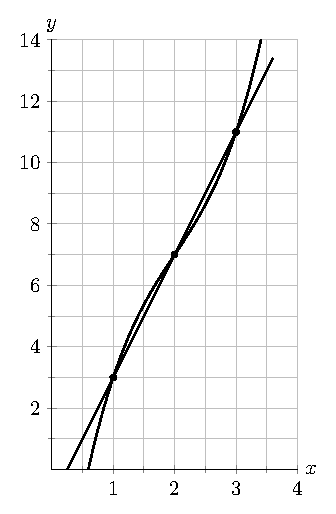
\includegraphics[width=.92\linewidth]{../figures/fhsm_2009_p38_1.pdf}
  \end{center}
  
  \item [Teacher:] Can you see now how you might find another polynomial graphically?
  \item [Student:] Maybe I could figure out a way to change the shape of the cubic graph but keep the intersection points the same.
  \item [Teacher:] How would you do that algebraically?
  \item [Student:] I could try to stretch the difference between $f(x)$ and $g(x)$, which is 

  $$
    g(x) - f(x) = x^3 - 6x^2 + 11x - 6.
  $$

  I could triple that, for example, and add it back on to $f(x)$ and get 

  $$
    \begin{aligned}
      &4x - 1 + 3(x^3 - 6x^2 + 11x - 6) \\
      &\quad= 3x^3 - 18x^2 + 37x - 19.
    \end{aligned}
  $$

  \item [Teacher:] Excellent. Now I want to understand what is really going on here. Is there anything special about the polynomial $x^3 - 6x^2 + 11x - 6$ that makes this work?
  \item [Student:] Not that I can see.
  \item [Teacher:] Why don't you try factoring it on your CAS?
  \item [Student:] I get 
  
   $$
    \begin{aligned}
      &x^3 - 6x^2 + 11x - 6 \\
      &\quad = (x - 1)(x - 2)(x - 3).
    \end{aligned}
  $$

  Oh, I see. When I look at the factored form, I can see that the difference between $f(x)$ and $g(x)$ is $0$ at $x = 1, 2, \text{ and } 3$. So I could get many polynomials that generate the same sequence just by adding a multiple of this polynomial to $f(x)$.

  \item [Teacher:] What is the general form of such a polynomial?
  \item [Student:] It is 

  $$
    4x - 1 + k(x - 1)(x - 2)(x - 3),
  $$

  where $k$ can be any real number. When I look at my graphing program, I notice that as $k$ increases, the graph of the polynomial stretches away from the line.

  \begin{center}
  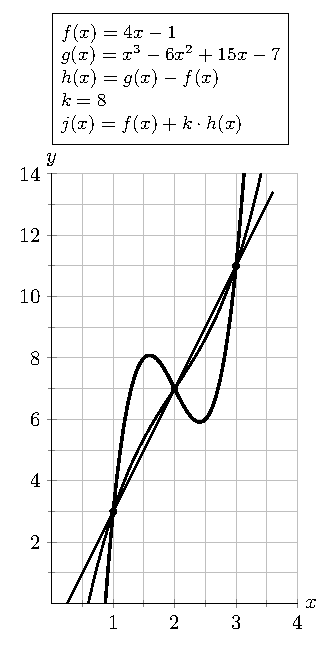
\includegraphics[width=.92\linewidth]{../figures/fhsm_2009_p39_2.pdf}
  \end{center}
\end{scriptlist}

\noindent
\textbf{Key Mathematical Elements}

Reasoning with Algebraic Symbols---Mindful manipulation; Linking expressions and functions

Reasoning with Functions---Using multiple representations of functions

\noindent
\textbf{Reasoning Habits}

Analyzing a problem---identifying relevant concepts, representations, or procedures; seeking patterns and relationships

Seeking and using connections
}
{
Chưa thấy hết quy luật
}
{
\noindent
\textbf{Nhiệm vụ}

Ở các lớp trước, có thể em đã gặp những bài toán yêu cầu tìm số hạng tiếp theo của một dãy, chẳng hạn $3$, $7$, $11$. Một câu trả lời có thể là $15$, nếu giả sử dãy được tạo ra bằng cách tính giá trị của $f(x)=4x-1$ tại $x=1,2,3$. Nhưng liệu còn có những câu trả lời khác không?

\noindent
\textbf{Trong lớp học (Toán năm thứ tư)}

\begin{scriptlist}
  \item [Giáo viên:] Hãy tìm dãy được tạo ra bằng cách tính $g(x)=x^3-6x^2+15x-7$ tại $x=1,2,3$.
  \item [Học sinh:] Em được $g(1)=3$, $g(2)=7$, và $g(3)=11$. Vẫn là cùng dãy ấy: $3$, $7$, $11$.
  \item [Giáo viên:] Nếu em dùng $g(x)$ thay cho $f(x)$ thì số hạng tiếp theo sẽ là gì?
  \item [Học sinh:] Khi đó sẽ là $g(4)=21$. Khác với kết quả nhận được khi dùng $f(x)$.
  \item [Giáo viên:] Em có thể tìm những đa thức khác cũng sinh ra dãy $3$, $7$, $11$ không?
  \item [Học sinh:] Em không hiểu ngay từ đầu làm sao thầy lại nghĩ ra được cái đa thức bậc ba lạ như vậy cho $g$.
  \item [Giáo viên:] Khi ta nói $g(1)=3$ thì điều đó có nghĩa là gì?
  \item [Học sinh:] Dạ, nghĩa là giá trị $y$, hay đầu ra, bằng $3$ khi giá trị $x$, hay đầu vào, bằng $1$.
  \item [Giáo viên:] Vậy thì làm sao hai hàm khác nhau, $f$ và $g$, lại có cùng giá trị tại $x=1,2,\text{ và }3$?
  \item [Học sinh:] Em đoán là cả hai đồ thị của chúng phải có cùng giá trị $y$.... À, nghĩa là chúng phải cắt nhau tại ba điểm ấy! Để em kiểm tra bằng cách vẽ đồ thị. Đúng rồi, khi em vẽ ra thì thấy đồ thị đường thẳng của $f(x)$ cắt đồ thị bậc ba của $g(x)$ tại $x=1,2,\text{ và }3$.

  \begin{center}
  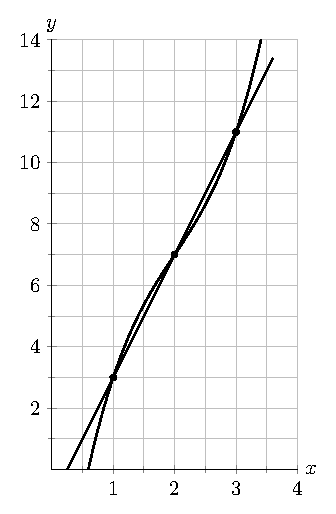
\includegraphics[width=.92\linewidth]{../figures/fhsm_2009_p38_1.pdf}
  \end{center}

  \item [Giáo viên:] Bây giờ em có thấy mình có thể tìm một đa thức khác bằng cách nhìn hình không?
  \item [Học sinh:] Có lẽ em có thể tìm cách làm thay đổi dạng của đồ thị bậc ba nhưng vẫn giữ nguyên các giao điểm.
  \item [Giáo viên:] Về mặt đại số, em sẽ làm điều đó thế nào?
  \item [Học sinh:] Em có thể thử kéo giãn hiệu giữa $f(x)$ và $g(x)$, tức là

  $$
    g(x)-f(x)=x^3-6x^2+11x-6.
  $$

  Chẳng hạn, em có thể nhân hiệu đó với $3$, rồi cộng trở lại vào $f(x)$ để được

  $$
    \begin{aligned}
      &4x-1+3(x^3-6x^2+11x-6) \\
      &\quad=3x^3-18x^2+37x-19.
    \end{aligned}
  $$

  \item [Giáo viên:] Rất tốt. Bây giờ thầy muốn hiểu điều gì thực sự đang diễn ra ở đây. Có điều gì đặc biệt ở đa thức $x^3-6x^2+11x-6$ khiến cách này hoạt động không?
  \item [Học sinh:] Em chưa thấy.
  \item [Giáo viên:] Sao em không thử phân tích nó thành nhân tử trên CAS?
  \item [Học sinh:] Em được

  $$
    \begin{aligned}
      &x^3-6x^2+11x-6 \\
      &\quad=(x-1)(x-2)(x-3).
    \end{aligned}
  $$

  À, em hiểu rồi. Khi nhìn dạng đã phân tích, em thấy hiệu giữa $f(x)$ và $g(x)$ bằng $0$ tại $x=1,2,\text{ và }3$. Vậy nên em có thể tạo ra nhiều đa thức cho cùng một dãy chỉ bằng cách cộng vào $f(x)$ một bội của đa thức này.

  \item [Giáo viên:] Dạng tổng quát của một đa thức như thế là gì?
  \item [Học sinh:] Đó là

  $$
    4x-1+k(x-1)(x-2)(x-3),
  $$

  trong đó $k$ có thể là bất kì số thực nào. Khi nhìn trên phần mềm vẽ đồ thị, em nhận thấy rằng khi $k$ tăng lên, đồ thị của đa thức càng tách xa khỏi đường thẳng.

  \begin{center}
    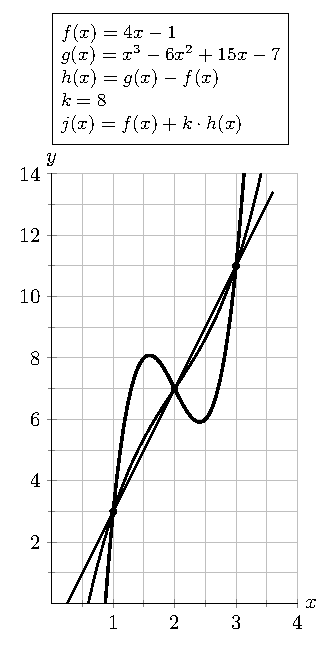
\includegraphics[width=.92\linewidth]{../figures/fhsm_2009_p39_2.pdf}
  \end{center}
\end{scriptlist}

\noindent
\textbf{Các yếu tố then chốt của toán học}

Luận với kí hiệu đại số---Biến đổi một cách tỉnh táo; Liên kết biểu thức với hàm số

Luận với hàm số---Sử dụng nhiều biểu diễn của hàm số

\noindent
\textbf{Các thói quen luận}

Phân tích bài toán---xác định các khái niệm, thủ tục, hoặc biểu diễn toán học thích đáng; tìm kiếm các mẫu hình và quan hệ

Tìm kiếm và sử dụng các kết nối
}
{}

% =========
% CHƯƠNG 6
% =========

\ParallelChapter
  {Reasoning with Functions}
  {Luận với hàm số}
  {}

\TriPara
{
\EN{Functions are one of the most important mathematical tools for helping students make sense of the world around them, as well as preparing them for further study in mathematics (Yerushalmy and Shternberg 2001). Functions appear in most branches of mathematics and provide a consistent way of making connections between and among topics. Students' continuing development of the concept of function must be rooted in reasoning, and likewise functions are an important tool for reasoning. Thus, developing procedural fluency in using functions is a significant goal of high school mathematics.

Key elements of reasoning and sense making with functions include the following:

\begin{itemize}
  \item \emph{Using multiple representations of functions.} Representing functions in various ways, including tabular, graphic, symbolic (explicit and recursive), visual, and verbal; making decisions about which representations are most helpful in problem-solving circumstances; and moving flexibly among those representations.
  \item \emph{Modeling by using families of functions.} Working to develop a reasonable mathematical model for a particular contextual situation by applying knowledge of the characteristic behaviors of different families of functions.
  \item \emph{Analyzing the effects of parameters.} Using a general representation of a function in a given family (e.g., the vertex form of a quadratic, $f(x) = a(x - h)2 + k$) to analyze the effects of varying coefficients or other parameters; converting between different forms of functions (e.g., the standard form of a quadratic and its factored form) according to the requirements of the problem-solving situation (e.g., finding the vertex of a quadratic or finding its zeros).
\end{itemize}

We address these key elements in more detail in the following sections.}
}
{
\VI{Các hàm số là một trong những công cụ toán học quan trọng nhất để giúp học sinh hiểu thế giới xung quanh mình, đồng thời chuẩn bị cho các em tiếp tục học toán ở trình độ cao hơn (Yerushalmy and Shternberg 2001). Hàm số xuất hiện trong hầu hết các ngành của toán học và cung cấp một cách nhất quán để tạo ra các kết nối giữa các chủ đề. Sự phát triển liên tục của khái niệm hàm số ở học sinh phải được đặt nền trên luận, và ngược lại, hàm số cũng là một công cụ quan trọng cho luận. Vì vậy, việc phát triển sự thành thạo thủ tục trong sử dụng hàm số là một mục tiêu quan trọng của toán học trung học phổ thông.

Các yếu tố then chốt của luận và hiểu với hàm số gồm có:
\begin{itemize}
\item \emph{Sử dụng nhiều biểu diễn của hàm số.} Biểu diễn hàm số theo nhiều cách khác nhau, bao gồm bằng bảng, đồ thị, kí hiệu (tường minh và truy hồi), hình ảnh trực quan, và lời; đưa ra quyết định về biểu diễn nào là hữu ích nhất trong từng tình huống giải quyết vấn đề; và chuyển đổi linh hoạt giữa các biểu diễn ấy.
\item \emph{Mô hình hóa bằng các họ hàm số.} Xây dựng một mô hình toán học hợp lí cho một tình huống ngữ cảnh cụ thể bằng cách vận dụng hiểu biết về những đặc trưng hành vi của các họ hàm số khác nhau.
\item \emph{Phân tích ảnh hưởng của các tham số.} Sử dụng một biểu diễn tổng quát của một hàm số trong một họ đã cho (chẳng hạn dạng đỉnh của một hàm bậc hai, $f(x)=a(x-h)^2+k$) để phân tích ảnh hưởng của việc thay đổi các hệ số hoặc các tham số khác; chuyển đổi giữa các dạng khác nhau của hàm số (chẳng hạn dạng chuẩn của một hàm bậc hai và dạng phân tích thành nhân tử của nó) tùy theo yêu cầu của tình huống giải quyết vấn đề (chẳng hạn tìm đỉnh của một hàm bậc hai hoặc tìm các nghiệm của nó).
\end{itemize}

Chúng tôi sẽ trình bày chi tiết hơn các yếu tố then chốt này trong những phần tiếp theo.}
}
{
\NOTE{}
}

\ParallelSection
  {Using Multiple Representations of Functions}
  {Sử dụng nhiều biểu diễn của hàm số}
  {}

\TriPara
{
\EN{Different representations of a function---tables, graphs or diagrams, symbolic expressions, and verbal descriptions---exhibit different properties. Using a variety of representations can help make functions more understandable to a wider range of students than can be accomplished by working with symbolic representations alone (Lloyd and Wilson 1998; Coulombe and Berenson 2001). Students need to establish connections among different representations, for example, the relationship among the zeros of a function, the solution of an equation, and the $x$-intercepts of graphs.}
}
{
\VI{Các biểu diễn khác nhau của một hàm số---bảng, đồ thị hoặc sơ đồ, biểu thức kí hiệu, và mô tả bằng lời---làm lộ ra những tính chất khác nhau. Việc sử dụng nhiều biểu diễn có thể giúp hàm số trở nên dễ hiểu hơn đối với một phổ học sinh rộng hơn so với khi chỉ làm việc với riêng các biểu diễn kí hiệu (Lloyd and Wilson 1998; Coulombe and Berenson 2001). Học sinh cần thiết lập được các kết nối giữa những biểu diễn khác nhau ấy, chẳng hạn như mối liên hệ giữa các nghiệm của một hàm số, nghiệm của một phương trình, và các giao điểm của đồ thị với trục $x$.}
}
{
\NOTE{}
}

\TriPara
{
\EN{Functions whose domains are the natural numbers are often represented recursively, where $f(k + 1)$ is defined in terms of $f(k)$ and an initial function value is given. Such functions can also be presented as sequences, and they are used in applications involving discrete rather than continuous data, often with the support of a calculator or an electronic spreadsheet; see example 10, ``Patterns, Plane and Symbol,'' and example 11, ``Take As Directed.''}
}
{
\VI{Những hàm số có miền xác định là các số tự nhiên thường được biểu diễn dưới dạng truy hồi, trong đó $f(k+1)$ được xác định theo $f(k)$ và một giá trị khởi đầu của hàm số được cho trước. Những hàm số như vậy cũng có thể được trình bày dưới dạng dãy số, và chúng được dùng trong những ứng dụng liên quan đến dữ liệu rời rạc hơn là dữ liệu liên tục, thường với sự hỗ trợ của máy tính cầm tay hoặc bảng tính điện tử; xem Ví dụ 10, ``Thêm đường thêm miền'', và Ví dụ 11, ``Uống theo chỉ dẫn''.}
}
{
\NOTE{}
}

\TriPara
{
\EN{One interesting exploration is to investigate the number of regions into which a plane is divided by $n$ straight lines. The first question is whether $n$ lines always divide the plane into the same number of regions. Experiments with two or three lines should help students see that different numbers of regions result. For example, two lines that cross create four regions, whereas two parallel lines create only three. Three parallel lines produce four regions; three lines all going through the same point create six regions; but three nonparallel, nonconcurrent lines create seven regions. In general, $n$ parallel lines create only $n + 1$ regions, whereas $n$ lines that all pass through the same point create $2n$ regions. The next example explores what happens in the case of nonparallel, nonconcurrent lines. It could be used with students entering high school, who are beginning to develop the ability to express functional relationships symbolically, or with more advanced students who are working to improve their profi ciency with algebraic manipulation. Example 10 illustrates how students can use various representations of functions, including verbal descriptions, tables, formulas, and various geometric models to make sense of a problem.}
}
{
\VI{Một hướng khám phá thú vị là khảo sát số miền mà một mặt phẳng bị chia thành bởi $n$ đường thẳng. Câu hỏi đầu tiên đặt ra là: liệu $n$ đường thẳng luôn chia mặt phẳng thành cùng một số miền hay không. Những thử nghiệm với hai hoặc ba đường thẳng sẽ giúp học sinh nhận ra rằng các cách bố trí khác nhau dẫn đến số miền khác nhau. Chẳng hạn, hai đường thẳng cắt nhau tạo ra bốn miền, trong khi hai đường thẳng song song chỉ tạo ra ba miền. Ba đường thẳng song song tạo ra bốn miền; ba đường thẳng cùng đi qua một điểm tạo ra sáu miền; còn ba đường thẳng không song song và không đồng quy tạo ra bảy miền. Nói chung, $n$ đường thẳng song song chỉ tạo ra $n+1$ miền, trong khi $n$ đường thẳng cùng đi qua một điểm tạo ra $2n$ miền. Ví dụ tiếp theo sẽ khảo sát trường hợp các đường thẳng không song song và không đồng quy. Hoạt động này có thể được sử dụng với học sinh mới bước vào trung học phổ thông, khi các em đang bắt đầu phát triển khả năng biểu diễn các mối quan hệ hàm số bằng ký hiệu, hoặc với những học sinh ở trình độ cao hơn đang rèn luyện sự thành thạo trong biến đổi đại số. Ví dụ 10 minh họa cách học sinh có thể sử dụng nhiều biểu diễn khác nhau của hàm số, bao gồm mô tả bằng lời, bảng, công thức và các mô hình hình học khác nhau, để kiến tạo ý nghĩa cho một bài toán.}
}
{
\NOTE{}
}

\TriExample
{Patterns, Plane and Symbol}
{
\noindent
\textbf{Task}

Develop a symbolic representation for a function that produces the number of regions in a plane formed by intersecting lines such that no two lines are parallel and no more than two lines intersect in the same point, as shown in the figure.

  \begin{center}
    \includegraphics[width=.92\linewidth]{../figures/fhsm_2009_p42_1_en.pdf}
  \end{center}

\noindent
\textbf{In the Classroom}

Students may approach this problem in several different ways, depending on their level of mathematical experience.

\begin{description}
  \item[Method 1.] After exploring a number of cases, possibly using an interactive geometry tool, students may produce a table of values for the number of lines, $L$, and the number of regions, $R$, as shown here:
    \begin{center}
    \setlength{\tabcolsep}{4pt}
    \begin{tabular}{|l|c|c|c|c|c|c|}
    \hline
    \shortstack[l]{No. of lines ($L$)} 
      & 1 & 2 & 3 & 4 & 5 & 6 \\
    \hline
    \shortstack[l]{No. of regions ($R$)} 
      & 2 & 4 & 7 & 11 & 16 & 22 \\
    \hline
    \end{tabular}
    \end{center}
  Students commonly observe the pattern of differences between consecutive terms of a sequence. This observation lends itself to a recursive definition of a function. In this example, a recursive definition would be $R(1) = 2, R(L) = R(L - 1) + L$.
  \item[Method 2.] An interesting geometric approach to helping students reason about this problem is to use checkers, coins, tiles, or other small objects to create a pattern in which the value of $L$ defines the number of rows of objects and the value of $R$ defines the total number of objects in the figure, as shown in the following sequence:
  
    \begin{center}
      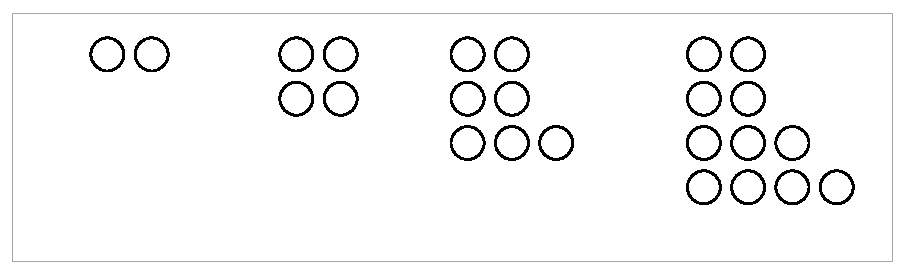
\includegraphics[width=.92\linewidth]{../figures/fhsm_2009_p43_1.pdf}
    \end{center}

  Removing one of the objects from the top row results in a triangular pattern, as shown below:
    
    \begin{center}
      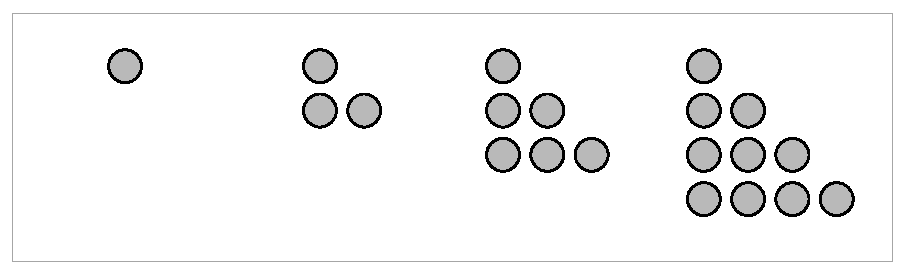
\includegraphics[width=.92\linewidth]{../figures/fhsm_2009_p43_2.pdf}
    \end{center}
  
  Doubling and transforming this pattern can result in a rectangle containing $L(L + 1)$ objects, as shown here:

    \begin{center}
      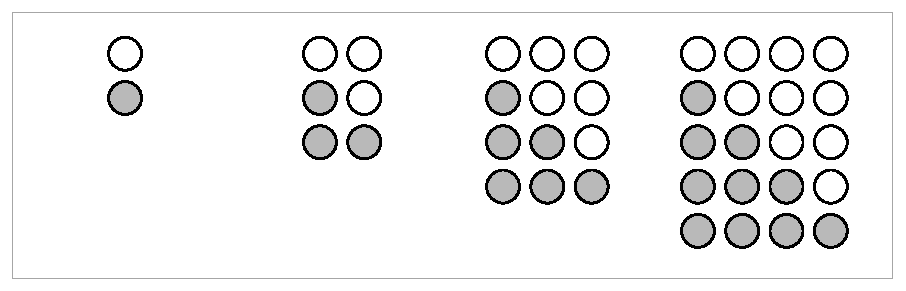
\includegraphics[width=.92\linewidth]{../figures/fhsm_2009_p43_3.pdf}
    \end{center}

  From this configuration, one can see that the original objects, minus the one that was removed, form half the rectangle. The explicit definition of this function can then be written as

  $$
  R=\frac{1}{2}(L)(L+1)+1=\frac{1}{2}L^2+\frac{1}{2}+1.
  $$

  This type of approach demonstrates how a student who is given the opportunity to represent a function pictorially can use a simple geometric pattern to write the explicit definition of the function. The student can then extend his or her reasoning about symbolic representations by developing it from a familiar starting place.
  \item[Method 3.] By applying technology to numeric and graphical reasoning, students may enter a number of ordered pairs from the table into a graphing calculator and examine a scatterplot of the pairs to conjecture that the relationship is quadratic because of the parabolic shape of the graph. On the basis of that conjecture, students could use calculator-assisted quadratic regression to find the function $R = 0.5L^2 + 0.5L + 1$. This algebraic model could be tested by using ordered pairs from the table.
  \item[Method 4.] The teacher could ask students to focus on the differences between consecutive terms of the sequence of R values: 2, 3, 4, 5, and so forth. By applying algebraic reasoning, students may examine the data and observe that the function is quadratic because the first differences are linear so the second differences are constant. The geometric representation shown in part 1 of this example can be used to reinforce this concept for students. Writing a system of equations of the form $R = aL^2 + bL + c$, substituting three ordered pairs, and solving the system would reveal that

  $$
    \begin{aligned}
      a=\frac{1}{2}, \; b=\frac{1}{2}, \; \text{and} \; c=1; \; \text{thus}\\
      R=\frac{1}{2}L^2+\frac{1}{2}L+1.
    \end{aligned}
  $$

This strategy would require a sophisticated understanding of several mathematical topics and a command of algebraic manipulation developed later in the high school experience.
\end{description}

\noindent
\textbf{Key Elements of Mathematics}

Reasoning with Functions---Using multiple representations of functions

Reasoning with Algebraic Symbols---Connecting algebra with geometry; Linking expressions and functions

\noindent
\textbf{Reasoning Habits}

Analyzing a problem---seeking patterns and relationships

Seeking and using connections

Reflecting on a solution---justifying or validating a solution
}
{Thêm đường thêm miền}
{
\noindent
\textbf{Nhiệm vụ}

Hãy xây dựng một biểu diễn kí hiệu cho một hàm số cho biết số miền của mặt phẳng được tạo thành bởi các đường thẳng cắt nhau, sao cho không có hai đường thẳng nào song song và không có quá hai đường thẳng nào cùng đi qua một điểm, như trong hình vẽ.

  \begin{center}
    \includegraphics[width=.92\linewidth]{../figures/fhsm_2009_p42_1_en.pdf}
  \end{center}

\noindent
\textbf{Trong lớp học}

Học sinh có thể tiếp cận bài toán này theo nhiều cách khác nhau, tùy thuộc vào mức độ trải nghiệm toán học của các em.

\begin{description}
  \item[Phương pháp 1.] Sau khi khảo sát một số trường hợp, có thể với sự hỗ trợ của một công cụ hình học tương tác, học sinh có thể lập một bảng giá trị cho số đường thẳng $L$ và số miền $R$, như sau:
    \begin{center}
    \setlength{\tabcolsep}{4pt}
    \begin{tabular}{|l|c|c|c|c|c|c|}
    \hline
    \shortstack[l]{Số đường thẳng ($L$)} 
      & 1 & 2 & 3 & 4 & 5 & 6 \\
    \hline
    \shortstack[l]{Số miền ($R$)} 
      & 2 & 4 & 7 & 11 & 16 & 22 \\
    \hline
    \end{tabular}
    \end{center}
  Học sinh thường nhận ra quy luật của hiệu giữa các số hạng liên tiếp của một dãy. Quan sát này dẫn tự nhiên đến một định nghĩa truy hồi của hàm số. Trong ví dụ này, một định nghĩa truy hồi sẽ là $R(1)=2,\; R(L)=R(L-1)+L$.
  \item[Phương pháp 2.] Một cách tiếp cận hình học thú vị để giúp học sinh luận về bài toán này là dùng quân cờ, đồng xu, các mảnh ghép, hoặc những vật nhỏ khác để tạo ra một mẫu hình trong đó giá trị của $L$ xác định số hàng đối tượng còn giá trị của $R$ xác định tổng số đối tượng trong hình, như trong dãy hình sau:
  
    \begin{center}
      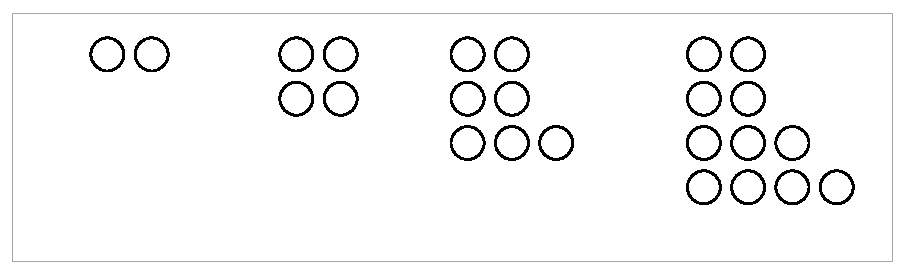
\includegraphics[width=.92\linewidth]{../figures/fhsm_2009_p43_1.pdf}
    \end{center}

  Nếu bỏ đi một đối tượng ở hàng trên cùng, ta được một mẫu hình tam giác, như dưới đây:
    
    \begin{center}
      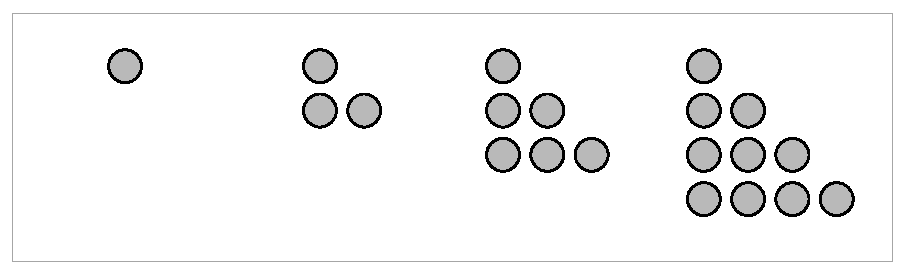
\includegraphics[width=.92\linewidth]{../figures/fhsm_2009_p43_2.pdf}
    \end{center}
  
  Gấp đôi và biến đổi mẫu hình này có thể tạo thành một hình chữ nhật chứa $L(L+1)$ đối tượng, như sau:

    \begin{center}
      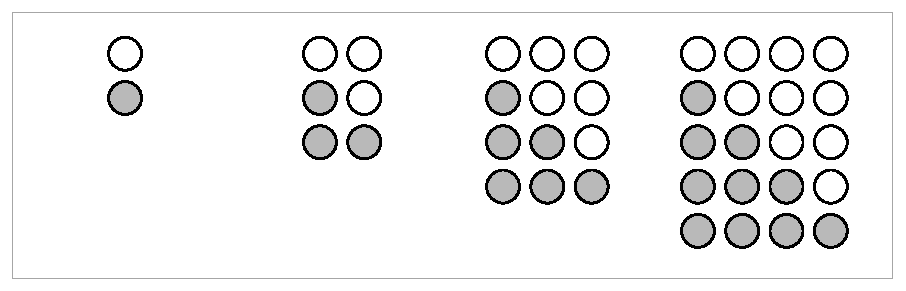
\includegraphics[width=.92\linewidth]{../figures/fhsm_2009_p43_3.pdf}
    \end{center}

  Từ cấu hình này, có thể thấy rằng các đối tượng ban đầu, sau khi bớt đi đối tượng đã bị lấy ra, tạo thành một nửa hình chữ nhật. Khi đó, công thức tường minh của hàm số có thể được viết là

  $$
  R=\frac{1}{2}(L)(L+1)+1=\frac{1}{2}L^2+\frac{1}{2}+1.
  $$

  Kiểu tiếp cận này cho thấy rằng một học sinh được trao cơ hội biểu diễn hàm số bằng hình ảnh có thể dùng một mẫu hình hình học đơn giản để viết ra công thức tường minh của hàm số. Từ đó, học sinh có thể mở rộng luận của mình về các biểu diễn kí hiệu bằng cách phát triển chúng từ một điểm khởi đầu quen thuộc.
  \item[Phương pháp 3.] Bằng cách dùng công nghệ để hỗ trợ luận bằng số và bằng đồ thị, học sinh có thể nhập một số cặp có thứ tự từ bảng vào máy tính vẽ đồ thị và quan sát đồ thị phân tán của các cặp điểm để phỏng đoán rằng quan hệ này là bậc hai do đồ thị có dạng parabol. Từ phỏng đoán ấy, học sinh có thể dùng phép hồi quy bậc hai với sự hỗ trợ của máy tính để tìm hàm số $R=0.5L^2+0.5L+1$. Mô hình đại số này có thể được kiểm tra bằng cách dùng các cặp có thứ tự trong bảng.
  \item[Phương pháp 4.] Giáo viên có thể yêu cầu học sinh tập trung vào hiệu giữa các số hạng liên tiếp của dãy các giá trị $R$: $2, 3, 4, 5$, v.v.. Bằng cách vận dụng luận đại số, học sinh có thể xem xét dữ liệu và nhận ra rằng hàm số là bậc hai vì sai phân bậc nhất là tuyến tính nên sai phân bậc hai là hằng số. Biểu diễn hình học ở phần 1 của ví dụ này có thể được dùng để củng cố ý tưởng ấy cho học sinh. Viết một hệ phương trình có dạng $R=aL^2+bL+c$, thay vào ba cặp có thứ tự, rồi giải hệ sẽ cho thấy rằng

  $$
    \begin{aligned}
      a=\frac{1}{2}, \; b=\frac{1}{2}, \; \text{and} \; c=1; \; \text{thus}\\
      R=\frac{1}{2}L^2+\frac{1}{2}L+1.
    \end{aligned}
  $$

Chiến lược này đòi hỏi sự hiểu biết tinh vi về nhiều chủ đề toán học và một năng lực biến đổi đại số thường chỉ được phát triển ở giai đoạn muộn hơn của trung học phổ thông.
\end{description}

\noindent
\textbf{Các yếu tố then chốt của toán học}

Luận với hàm số---Sử dụng nhiều biểu diễn của hàm số

Luận với kí hiệu đại số---Kết nối đại số với hình học; Liên kết biểu thức với hàm số

\noindent
\textbf{Các thói quen luận}

Phân tích bài toán---tìm kiếm các mẫu hình và quan hệ

Tìm kiếm và sử dụng các kết nối

Phản tư về lời giải---biện minh hoặc kiểm chứng một lời giải
}
{}

\ParallelSection
  {Modeling by Using Families of Functions}
  {Mô hình hóa bằng cách sử dụng họ hàm số}
  {}

\TriPara
{
\EN{According to Curriculum Focal Points (NCTM 2006a), students should enter high school having had extensive experience with linear functions and some exposure to nonlinear functions. High school experiences can help students build on this knowledge and work with parameterized families of functions (e.g., linear, quadratic, exponential, and periodic), each of which has distinguishing characteristics common to all members of the family. Given data from a problem situation, students should be able to (a) choose a family of functions that sensibly models the situation; (b) find parameters for a function to approximately match the data; (c) use the resulting function to solve the problem; and (d) interpret and refl ect on their solution in the context of the problem.}
}
{
\VI{Theo Curriculum Focal Points (NCTM 2006a), học sinh khi bước vào trung học phổ thông đã có nhiều trải nghiệm với các hàm tuyến tính và có sự làm quen nhất định với các hàm phi tuyến. Các hoạt động học tập ở bậc trung học phổ thông có thể giúp học sinh phát triển trên nền tảng đó và làm việc với các họ hàm số có tham số (chẳng hạn như hàm tuyến tính, hàm bậc hai, hàm mũ và hàm tuần hoàn), trong đó mỗi họ hàm đều có những đặc trưng riêng chung cho tất cả các phần tử của họ. Khi được cung cấp dữ liệu từ một tình huống bài toán, học sinh cần có khả năng: (a) lựa chọn một họ hàm số phù hợp để mô hình hóa tình huống đó; (b) xác định các tham số của một hàm sao cho xấp xỉ tốt với dữ liệu; (c) sử dụng hàm số thu được để giải quyết bài toán; và (d) diễn giải và suy ngẫm về lời giải của mình trong bối cảnh của bài toán.}
}
{
\NOTE{}
}

\TriPara
{
\EN{Using problems that can be extended and revisited as students mature is a powerful way to help students make connections between existing knowledge and new learning. Example 11 uses a context to which students can readily relate and demonstrates how a problem can be extended as students' mathematical backgrounds become more sophisticated. It also shows the power of deductive reasoning in developing a general solution to a problem.}
}
{
\VI{Việc sử dụng những bài toán có thể được mở rộng và quay lại khai thác ở các giai đoạn phát triển khác nhau của học sinh là một cách hiệu quả để giúp các em thiết lập mối liên hệ giữa kiến thức đã có và kiến thức mới. Ví dụ 11 sử dụng một bối cảnh quen thuộc, dễ liên hệ đối với học sinh, và minh họa cách một bài toán có thể được mở rộng dần khi nền tảng toán học của học sinh trở nên vững vàng và tinh vi hơn. Ví dụ này cũng cho thấy sức mạnh của luận suy diễn trong việc xây dựng một lời giải tổng quát cho bài toán.}
}
{
\NOTE{}
}

% ----------
% VÍ DỤ 11
% ----------

\TriExample
{
Take As Directed
}
{
\noindent
\textbf{Task}

A student strained her knee in an intramural volleyball game, and her doctor has prescribed an anti-inflammatory drug to reduce the swelling. The student takes two 220 mg tablets every 8 hours for 10 days. Her kidneys eliminate $60$ percent of this drug from her body every 8 hours. Determine how much of the drug is in her system after 10 days, just after she takes her last dose of medicine. Explain what happens to the change in the amount of medicine in the body as time progresses and why this pattern occurs. If she continued to take the drug for a year, how much of the drug would be in her system just after she took her last dose? Explain, in mathematical terms and in terms of body metabolism, why the long-term amount of medicine in the body is reasonable (adapted from NCTM [2000b]).

\noindent
\textbf{In the Classroom (Variety of Levels from First-Year to Fourth-Year Mathematics)}

Students may examine this problem in varying degrees of depth, depending on their level of mathematical experience:

\begin{description}
  \item[Method 1.] Students who are near the beginning of their high school experience could produce a table of data and generate a discrete graph of the data. The following table and graph show the amount of medicine, $A_n$, in mg, in the athlete's body just after taking $n$ doses of medicine.
  
  \begin{center}
  \setlength{\tabcolsep}{5pt}
  \begin{tabular}{|c|c|c|c|c|}
  \hline
  $n$   & $1$      & $2$      & $3$      & $4$      \\
  \hline
  $A_n$ & $440$    & $616$    & $686.40$ & $714.56$ \\
  \hline
  $n$   & $5$      & $6$      & $7$      & $8$      \\
  \hline
  $A_n$ & $725.82$ & $730.33$ & $732.13$ & $732.85$ \\
  \hline
  $n$   & $9$      & $10$     & $11$     & $12$     \\
  \hline
  $A_n$ & $733.14$ & $733.26$ & $733.30$ & $733.32$ \\
  \hline
  $n$   & $\dots$  & $20$     & $\dots$  & $30$     \\
  \hline
  $A_n$ & $\dots$  & $733.33$ & $\dots$  & $733.33$ \\
  \hline
  \end{tabular}
  \end{center}

  Students may observe that the level of medicine in the body initially rises rapidly but with time increases less rapidly. Thus, the rate of change of this function does not remain constant. Even a beginning student could surmise from this table that the medicine level appears to eventually stabilize, so that after about seventeen dosage periods, the value no longer seems to change. In terms of metabolism, students could explain that the athlete's body is eliminating the same amount of medication as she is taking in each dose. This observation can be mathematically verified by showing that

  $$
  0.6\left(733\frac{1}{3}\right)=440
  $$

  because the value of $A_n$ approaches a limiting value of
  
  $$
  733\frac{1}{3} \, \text{mg}
  $$

  after about seventeen doses.

  \begin{center}
      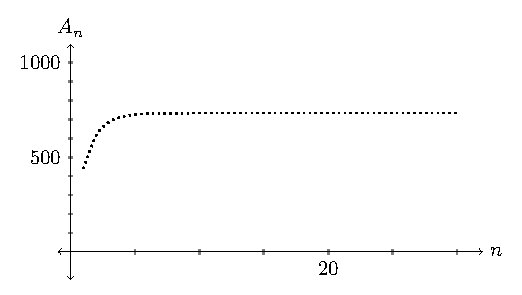
\includegraphics[width=.92\linewidth]{../figures/fhsm_2009_p46_1.pdf}
  \end{center}
  \item[Method 2.] A problem such as this can be expressed in recursive notation. A recursive definition for the sequence of medicine levels in the athlete's body would be $A_{n+1} = 0.40A_n + 440$, $A_1 = 0$. Obtaining explicit formulas from tables of data is often quite difficult and in some situations, impossible. A recursive approach, especially when supported by a calculator or an electronic spreadsheet, is more intuitive and gives students access to such interesting problems as this earlier in their schooling.
  \item[Method 3.] Students who are studying exponential functions might use a problem such as this to develop their understanding of exponential decay. By examining the pattern of medicine levels, students can observe that the change of medicine level in the athlete's body is decreasing; specifically, each change is $40$ percent of the previous amount of change. After reasoning about the repetitive nature of multiplying by $0.4$, students could express this relationship with the explicit function

  $$
  I(n)=440(0.4^{n-1}),
  $$

  where $I(n)$ represents the increase in medicine level after dose number $n$. When students are ready, an illuminating exercise would be to verify this result formally, as follows:

  \begin{quotation}
    If a sequence $A_n$ satisfies a linear recursion $A_{n+1} = a \cdot A_n + b$ for some constants $a$ and $b$, then the differences $A_n +1 - A_n$ satisfy the simpler recursion

    \begin{align*}
      &A_{n+1}-A_n \\
      &\quad =(a\cdot A_n+b)-(a\cdot A_{n-1}+b) \\
      &\quad =a\cdot (A_n-A_{n-1}).
    \end{align*}

    Therefore, these differences are just powers of a times the first difference:

    $$
    A_{n+1}-A_n
      =a^n\cdot (A_1-A_0).
    $$
  \end{quotation}

  Note that we can show from this result that $A_n$ itself is the sum of a geometric progression. Thus, this kind of problem can provide another motivation for an application of geometric progressions.
  \item[Method 4.] For older students with a more sophisticated mathematical background, this problem could be revisited as a means of informally introducing them to the important mathematical concept of limit, especially when coupled with a discrete graph of the sequence, as shown in the graph on the previous page.
  \item[Method 5.] Students who have more experience with reasoning and sense making may be asked to formally justify why the level of medicine converges, thus creating a deeper understanding of the phenomenon and why it happens. In this approach to the problem, students are asked to use a formal proof to show that the sequence will converge for large numbers of doses. For instance, consider the recursive function for the amount $A$ of medicine in the athlete's body after $n$ doses:

  \begin{align*}
    A_{n+1}
      &=A_n-0.6A_n+440 \\
      &=0.4A_n+440. \tag{1}
  \end{align*} 

  We can define the behavior of the medicine level as a linear function $C$, called the \emph{transition function governing the sequence} $A_n$ , where

    \begin{align*}
      C(x)=0.4x+440. \tag{2}
    \end{align*} 

  By substitution, we can write

  \begin{align*}
    A_{n+1}
      &=0.4A_n+440 \\
      &=C(A_n). \tag{3}
  \end{align*} 

  Now if the medicine concentrations truly level off, we can let $V$ represent the fixed value approached by $A_n$ after a certain number of doses, called the \emph{fixed point of} $C$. Doing so leads to the equation

    \begin{align*}
      C(V)=V, \, \text{or} \, 0.4V+440=V. \tag{4}
    \end{align*} 

  Solving equation (4) for $V$ gives us the value

  $$
    V=7.33\frac{1}{3},
  $$

  which proves that the limiting value of the blood concentration is

  $$
    V=7.33\frac{1}{3} \, \text{mg}
  $$

  as explained by the transition function $C$, defined in equation (2).

  To see how the transition function guarantees the convergence, we can rewrite it to display the difference between the actual amount and the fixed value. Defi ne $D_n$ as the difference between the actual amount of medicine, $A_n$, and the fixed value, $V$:

    \begin{align*}
      A_n=V+D_n. \tag{5}
    \end{align*} 

  Substituting this result in the recursion relation, equation (3), gives

  \begin{align*}
    A_{n+1}
      &=0.4(V+D_n)+440\\
      &=(0.4+440)+0.4D_n. \tag{6}
  \end{align*} 

  Since $A_{n+1} = V + D_{n+1}$, from equation (5), and since $V$ is defined by the relation $V = 0.4V + 440$, from equation (4), we can reduce the relationship further:

  \begin{align*}
    &V+D_{n+1} \\
    &\quad =(0.4V+440)+0.4D_n, \\
    & (0.4V+440)+0.4D_{n+1} \\
    &\quad =(0.4V+440)+0.4D_n.  
  \end{align*}

  From this result we can derive the simple recursion

    \begin{align*}
      D_{n+1}=0.4D_n, \tag{7}
    \end{align*} 
  
  which shows that at each step, $D_n$ shrinks to 40 percent of its previous value. Clearly, after not too many steps, $D_n$ will become negligibly small, as was suggested by the foregoing numerical calculations.
\end{description}

\noindent
\textbf{Key Mathematical Elements}

Reasoning with Functions---Using multiple representations of functions; Modeling by using families of functions

Reasoning with Algebraic Symbols---Meaningful use of symbols; Mindful
manipulation

\noindent
\textbf{Reasoning Habits}

Analyzing a problem---identifying relevant concepts, procedures, or representations; seeking patterns and relationships

Implementing a strategy---making logical deductions

Reflecting on a solution---justifying or validating a solution
}
{
Uống theo chỉ dẫn
}
{
\noindent
\textbf{Nhiệm vụ}

Một học sinh bị căng khớp gối khi chơi bóng chuyền trong hoạt động thể thao nội bộ, và bác sĩ kê một loại thuốc kháng viêm để giảm sưng. Học sinh uống hai viên $220$ mg mỗi $8$ giờ trong $10$ ngày. Thận của học sinh loại bỏ $60$ phần trăm lượng thuốc này khỏi cơ thể sau mỗi $8$ giờ. Hãy xác định lượng thuốc có trong cơ thể sau $10$ ngày, ngay sau khi học sinh uống liều thuốc cuối cùng. Giải thích điều gì xảy ra đối với sự thay đổi của lượng thuốc trong cơ thể theo thời gian và vì sao mẫu hình này xuất hiện. Nếu học sinh tiếp tục uống thuốc trong một năm, thì ngay sau khi uống liều thuốc cuối cùng, lượng thuốc trong cơ thể sẽ là bao nhiêu? Hãy giải thích, theo các thuật ngữ toán học và theo cơ chế chuyển hóa của cơ thể, vì sao lượng thuốc dài hạn trong cơ thể là hợp lý (phỏng theo NCTM [2000b]).

\noindent
\textbf{Trong lớp học (nhiều mức độ: từ Toán năm thứ nhất đến Toán năm thứ tư)}

Học sinh có thể xem xét bài toán này ở những mức độ sâu khác nhau, tùy theo mức độ trải nghiệm toán học của các em:

\begin{description}
  \item[Phương pháp 1.] Những học sinh ở giai đoạn gần đầu bậc trung học phổ thông có thể lập một bảng dữ liệu và vẽ đồ thị rời rạc của dữ liệu. Bảng và đồ thị sau đây cho thấy lượng thuốc $A_n$ (tính theo mg) có trong cơ thể của vận động viên ngay sau khi uống $n$ liều thuốc.
  
  \begin{center}
  \setlength{\tabcolsep}{5pt}
  \begin{tabular}{|c|c|c|c|c|}
  \hline
  $n$   & $1$      & $2$      & $3$      & $4$      \\
  \hline
  $A_n$ & $440$    & $616$    & $686.40$ & $714.56$ \\
  \hline
  $n$   & $5$      & $6$      & $7$      & $8$      \\
  \hline
  $A_n$ & $725.82$ & $730.33$ & $732.13$ & $732.85$ \\
  \hline
  $n$   & $9$      & $10$     & $11$     & $12$     \\
  \hline
  $A_n$ & $733.14$ & $733.26$ & $733.30$ & $733.32$ \\
  \hline
  $n$   & $\dots$  & $20$     & $\dots$  & $30$     \\
  \hline
  $A_n$ & $\dots$  & $733.33$ & $\dots$  & $733.33$ \\
  \hline
  \end{tabular}
  \end{center}

  Học sinh có thể nhận thấy rằng nồng độ thuốc trong cơ thể ban đầu tăng nhanh, nhưng theo thời gian thì tăng chậm dần. Do đó, tốc độ thay đổi của hàm này không giữ nguyên là hằng số. Ngay cả một học sinh mới bắt đầu cũng có thể phỏng đoán từ bảng rằng nồng độ thuốc dường như sẽ ổn định về sau, đến mức sau khoảng mười bảy chu kỳ liều dùng thì giá trị dường như không còn thay đổi nữa. Về mặt chuyển hóa, học sinh có thể giải thích rằng cơ thể vận động viên đang loại bỏ đúng bằng lượng thuốc mà cô ấy đưa vào ở mỗi liều. Quan sát này có thể được kiểm chứng về mặt toán học bằng cách chỉ ra rằng

  $$
  0.6\left(733\frac{1}{3}\right)=440
  $$

  bởi vì $A_n$ tiến dần tới một giá trị giới hạn là
  
  $$
  733\frac{1}{3} \, \text{mg}
  $$

  sau khoảng mười bảy liều.

  \begin{center}
      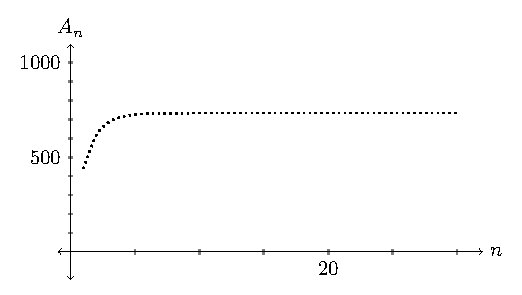
\includegraphics[width=.92\linewidth]{../figures/fhsm_2009_p46_1.pdf}
  \end{center}
  \item[Phương pháp 2.] Một bài toán như thế này có thể được biểu diễn bằng ký hiệu truy hồi. Một định nghĩa truy hồi cho dãy nồng độ thuốc trong cơ thể vận động viên là $A_{n+1}=0.40A_n+440,\, A_1=0$. Việc rút ra công thức tường minh từ các bảng dữ liệu thường rất khó, và trong một số tình huống là không thể. Phương pháp tiếp cận truy hồi, đặc biệt khi được hỗ trợ bởi máy tính cầm tay hoặc bảng tính điện tử, thường trực quan hơn và cho phép học sinh tiếp cận những bài toán thú vị như thế này từ sớm hơn trong quá trình học.
  \item[Phương pháp 3.] Những học sinh đang học về hàm mũ có thể dùng một bài toán như thế này để phát triển hiểu biết về sự suy giảm mũ. Khi xem xét mẫu hình các mức thuốc, học sinh có thể quan sát rằng mức tăng của lượng thuốc trong cơ thể đang giảm dần; cụ thể, mỗi mức tăng bằng $40$ phần trăm mức tăng ngay trước đó. Sau khi lập luận về bản chất lặp lại của việc nhân với $0.4$, học sinh có thể biểu diễn mối quan hệ này bằng hàm tường minh

  $$
  I(n)=440(0.4^{n-1}),
  $$

  trong đó $I(n)$ là mức tăng của lượng thuốc sau liều thứ $n$. Khi học sinh đã sẵn sàng, một bài tập làm sáng tỏ vấn đề là kiểm chứng kết quả này một cách hình thức như sau:
  
  \begin{quotation}
    Nếu một dãy $A_n$ thỏa một truy hồi tuyến tính $A_{n+1}=a\cdot A_n+b$ với một số hằng $a$ và $b$, thì các sai khác $A_{n+1}-A_n$ thỏa một truy hồi đơn giản hơn
    
    \begin{align*}
      &A_{n+1}-A_n \\
      &\quad =(a\cdot A_n+b)-(a\cdot A_{n-1}+b) \\
      &\quad =a\cdot (A_n-A_{n-1}).
    \end{align*}

    Do đó, các sai khác này chỉ là các lũy thừa của $a$ nhân với sai khác đầu tiên:
    
    $$
    A_{n+1}-A_n
      =a^n\cdot (A_1-A_0).
    $$
  \end{quotation}

  Lưu ý rằng từ kết quả này có thể suy ra $A_n$ là tổng của một cấp số nhân. Vì vậy, dạng bài toán này cung cấp thêm một động lực cho việc áp dụng cấp số nhân.
  \item[Phương pháp 4.] Với những học sinh lớn hơn, có nền tảng toán học tinh vi hơn, bài toán này có thể được quay lại như một cách để giới thiệu một cách không chính thức khái niệm toán học quan trọng về giới hạn, đặc biệt khi kết hợp với đồ thị rời rạc của dãy số như trong hình ở trang trước.
  \item[Phương pháp 5.] Những học sinh có nhiều trải nghiệm hơn với lập luận và kiến tạo ý nghĩa có thể được yêu cầu biện minh một cách hình thức vì sao mức thuốc hội tụ, qua đó hình thành sự hiểu biết sâu hơn về hiện tượng và lý do nó xảy ra. Trong cách tiếp cận này, học sinh được yêu cầu dùng một chứng minh hình thức để chỉ ra rằng dãy sẽ hội tụ khi số liều trở nên lớn. Chẳng hạn, xét hàm truy hồi cho lượng thuốc $A$ trong cơ thể vận động viên sau $n$ liều:

  \begin{align*}
    A_{n+1}
      &=A_n-0.6A_n+440 \\
      &=0.4A_n+440. \tag{1}
  \end{align*} 

  Ta có thể mô tả sự biến thiên của mức thuốc bằng một hàm tuyến tính $C$, gọi là \emph{hàm chuyển tiếp chi phối dãy} $A_n$, với

    \begin{align*}
      C(x)=0.4x+440. \tag{2}
    \end{align*} 

  Bằng phép thế, ta viết

  \begin{align*}
    A_{n+1}
      &=0.4A_n+440 \\
      &=C(A_n). \tag{3}
  \end{align*} 


  Bây giờ, nếu nồng độ thuốc thực sự tiến tới ổn định, ta có thể dùng $V$ để chỉ giá trị cố định mà $A_n$ tiến gần tới sau một số liều nhất định; giá trị này được gọi là \emph{điểm bất động của} $C$. Làm như vậy dẫn đến phương trình

  \begin{align*}
    C(V)=V, \, \text{or} \, 0.4V+440=V. \tag{4}
  \end{align*}

  Giải phương trình (4) theo $V$ cho ta giá trị 

  $$
    V=7.33\frac{1}{3},
  $$

  chứng tỏ rằng giá trị giới hạn của nồng độ thuốc trong máu là

  $$
    V=7.33\frac{1}{3} \, \text{mg}
  $$

  như được giải thích bởi hàm chuyển tiếp $C$ đã nêu trong (2).

  Để thấy vì sao hàm chuyển tiếp bảo đảm sự hội tụ, ta viết lại sao cho lộ ra độ lệch giữa lượng thực tế và giá trị cố định. Gọi $D_n$ là độ lệch giữa lượng thuốc thực tế $A_n$ và giá trị cố định $V$:

  \begin{align*}
      A_n=V+D_n. \tag{5}
  \end{align*}

  Thay kết quả này vào hệ thức truy hồi, tức phương trình (3), ta được

  \begin{align*}
    A_{n+1}
      &=0.4(V+D_n)+440\\
      &=(0.4+440)+0.4D_n. \tag{6}
  \end{align*} 

  Vì $A_{n+1}=V+D_{n+1}$ theo phương trình (5), và vì $V$ được xác định bởi hệ thức $V=0.4V+440$ theo phương trình (4), ta có thể rút gọn hệ thức ấy thêm nữa:

  \begin{align*}
    &V+D_{n+1} \\
    &\quad =(0.4V+440)+0.4D_n, \\
    & (0.4V+440)+0.4D_{n+1} \\
    &\quad =(0.4V+440)+0.4D_n.  
  \end{align*}

  Từ kết quả này, ta có thể suy ra hệ thức truy hồi đơn giản sau:

  \begin{align*}
      D_{n+1}=0.4D_n, \tag{7}
  \end{align*}
  
  hệ thức này cho thấy rằng ở mỗi bước, $D_n$ giảm xuống còn $40$ phần trăm giá trị của nó ở bước trước. Rõ ràng, chỉ sau không quá nhiều bước, $D_n$ sẽ trở nên nhỏ đến mức có thể xem như không đáng kể, đúng như các phép tính số ở trên đã gợi ra.
\end{description}

\noindent
\textbf{Các yếu tố then chốt của toán học}

Luận với hàm số---Sử dụng nhiều biểu diễn của hàm số; Mô hình hóa bằng các họ hàm số

Luận với ký hiệu đại số---Sử dụng ký hiệu có nghĩa; Biến đổi có ý thức

\noindent
\textbf{Các thói quen luận}

Phân tích bài toán---xác định các khái niệm, thủ tục, hoặc biểu diễn toán học thích đáng; tìm kiếm các mẫu hình và quan hệ  

Triển khai chiến lược---thực hiện những suy diễn có tính luận lý  

Phản tư về lời giải---biện minh hoặc kiểm chứng một lời giải
}
{
Ví dụ 11 cho thấy rõ giá trị của một bài toán có thể được quay lại nhiều lần ở những mức độ khác nhau của luận và hiểu. Cùng một bối cảnh---thuốc được bổ sung theo chu kỳ và bị đào thải theo một tỉ lệ cố định---có thể trước hết được đọc bằng bảng số và đồ thị rời rạc để làm lộ trực giác về sự ổn định, rồi được mô hình hóa bằng hệ thức truy hồi
$$
A_{n+1}=0.4A_n+440,
$$
sau đó được nhìn lại như một bài toán về suy giảm mũ, về giới hạn, và cuối cùng là về chứng minh hội tụ. Chính cấu trúc nhiều tầng này làm cho ví dụ trở thành một trục nối giữa mô hình hóa, hàm số, biểu diễn, và lập luận suy diễn. 

Điểm đáng chú ý nhất nằm ở sự khác nhau giữa Phương pháp 3 và Phương pháp 5. Ở Phương pháp 3, trọng tâm được chuyển sang mức tăng
$$
I(n)=A_n-A_{n-1},
$$
từ đó học sinh nhận ra một cấu trúc mũ: mỗi mức tăng mới chỉ còn $40$ phần trăm mức tăng trước. Cách nhìn này hiệu quả vì nó cho thấy vì sao lượng thuốc tăng chậm dần và mở ra một động lực tự nhiên cho việc học cấp số nhân. Tuy nhiên, nó vẫn còn dựa nhiều vào việc nhận ra một quy luật thuận lợi trong dữ liệu.

Phương pháp 5 đi xa hơn: thay vì theo dõi các mức tăng, nó xem toàn bộ bài toán như một phép lặp
$$
C(x)=0.4x+440.
$$
Khi đó, giá trị ổn định không còn chỉ là một con số được đoán ra từ bảng, mà là điểm bất động $V$ thỏa
$$
C(V)=V.
$$
Việc xét độ lệch $D_n=A_n-V$ và suy ra
$$
D_{n+1}=0.4D_n
$$
làm lộ cơ chế hội tụ một cách trực tiếp: khoảng cách tới trạng thái cân bằng bị thu nhỏ theo cùng một tỉ lệ sau mỗi chu kỳ. Ở đây, ``ổn định'' không còn là một quan sát số học, mà trở thành hệ quả của chính cấu trúc phép lặp.

Giá trị sư phạm của ví dụ vì thế không nằm riêng ở lời giải cho bài toán thuốc, mà ở cách nó cho phép cùng một tình huống nâng đỡ nhiều mức học khác nhau. Người mới học có thể bắt đầu từ bảng và đồ thị; học sinh khá hơn có thể nhận ra truy hồi và cấu trúc mũ; học sinh đã vững hơn có thể dùng điểm bất động để giải thích vì sao hội tụ xảy ra. Nhờ đó, ví dụ minh họa đúng tinh thần của sách: hiểu không tách rời luận, và cùng một bối cảnh tốt có thể được dùng để đưa người học từ trực giác đến biện giải chặt chẽ. 
}

\TriPara
{
\EN{Incorporating formal proof throughout the high school mathematics curriculum serves to strengthen students' reasoning skills and can also ease the transition from high school to college mathematics. The general reasoning in example 11, ``Take As Directed,'' can be extended to a range of other situations, as shown in example 12, which demonstrates an application of formal proof to the important context of finance. This example shows how students can grow in their own reasoning ability by studying and interpreting the reasoning of others.}
}
{
\VI{Việc lồng ghép chứng minh hình thức xuyên suốt chương trình toán học trung học phổ thông giúp củng cố năng lực lập luận của học sinh, đồng thời làm dịu đi bước chuyển tiếp từ toán học phổ thông lên toán học đại học. Luận tổng quát trong Ví dụ 11, “Uống theo chỉ dẫn”, có thể được mở rộng cho nhiều tình huống khác, như được minh họa trong Ví dụ 12, nơi trình bày một ứng dụng của chứng minh hình thức trong bối cảnh quan trọng của tài chính. Ví dụ này cho thấy học sinh có thể phát triển năng lực luận của chính mình thông qua việc nghiên cứu và diễn giải luận của người khác.}
}
{
\NOTE{}
}

\TriExample
{Money Matters}
{
\noindent
\textbf{Task}

After exploring the method of formal justification in example 11 (method 5), a teacher asks her students to read and interpret the following text describing how to determine the payment amount for installment loans, and to answer a series of questions about the text.

\begin{quotation}
  When someone takes out an installment loan, we need to be able to find the monthly payment amount so that the loan is paid off in a certain number of months. The monthly payment on an installment loan includes the interest charged on the unpaid amount of the loan (the principal) since the last payment. Any amount of the payment left over after the interest is deducted goes toward paying off the loan, thereby reducing the principal.

  Let's express this situation by using algebraic notation. Define $P_n$ to be the principal owed at the end of period $n$, where $P_0$ is the amount initially borrowed. If the interest rate for a single period is r and the borrower makes a monthly payment $M$ at the end of each period, then the principal owed at the end of the period $n + 1$ can be written as $P_n+1=P_n+rP_n-M=(1+r)P_n-M$. Thus, the principal owed at the end of one month is related to the principal owed the month before by the linear function $P_{n+1}=Q(P_n)$, where $Q(x)=(1+r)x-M$.

  If we want to pay the principal off in $m$ months, then $P_m = 0$. Noting that $P_m=Q(P_m-1) =Q(Q(P_{m-2})) = Q(Q(Q(P_{m-3})))$, and so forth, we can see that $P_m = Q^{(m)}(P_0) = 0$, where we use $PQ^{(m)}$ to stand for the composition of $Q$ with itself m times. If we can find an expression for $PQ^{(m)}(P_0)$ in terms of $P_0$, $M$, $m$, and $r$, we can solve the equation $Q^{(m)}(P_0) = 0$ for $M$ in terms of the given variables.

  However, finding the expression is not easy. We can use a fixed-point analysis to simplify the effect of $Q$. If $F$ is the fixed point of $Q$, then $Q(F) = F$. Thus, $Q(F)=(1+r)F-M = F$. So we can see that $F = M/r$.

  Next, let us define $D_n$ as the difference between $P_n$ and the fixed point $F$, that is,

  $$
    D_n=P_n-F, \, \text{or} \, P_n=F+D_n.
  $$

  Then, on the one hand,

  \begin{align*}
    Q(P_n)
      &=Q(F+D_n) \\
        & \text{(from our definition of $D_n$)} \\
      &=(1+r)(F+D_n)-M \\
        & \text{(by applying} \\
        & \text{the definition of $Q$)} \\
      &=((1 + r)F - M) + (1 + r)D_n \\
        & \text{(by distribution and} \\
        & \text{rearranging terms)} \\
      &=Q(F) + (1 + r)D_n \\
        & \text{(again by applying} \\
        & \text{the definition of $Q$)} \\
      &=F + (1 + r)D_n \\
        & \text{(since $F$ is} \\
        & \text{the fixed point for $Q$).}
  \end{align*}

On the other hand,

  \begin{align*}
    Q(P_n)
      &=P_{n+1} \\
        & \text{(by definition of $Q$)} \\
      &=F + D_{n+1} \\
        & \text{(by definition of $D_{n+1}$).}
  \end{align*}

  Equating the two expressions for $Q(P_n)$ gives

  \begin{align*}
    F+(1+r)D_n&=F+D_{n+1}, \, \text{or} \\
    D_{n+1}&=(1+r)D_n.
  \end{align*}

  Thus, $D_n$ , the difference between $P_n$ and the fixed point $F$, varies in a simpler way than $P_n$ does: it is simply multiplied by $(1 + r)$ at each step.

  Applying this relation twice gives

  \begin{align*}
    D_{n+2}
      &=(1+r)D_{n+1} \\
        & \text{(by substituting $n + 1$ for $n$)} \\
      &=(1+r)((1+r)D_n) \\
        & \text{(by the equation for $n$)} \\
      &=(1+r)^2D_n \\
        & \text{(by the associative rule and} \\
        & \text{the definition of exponents).}
  \end{align*}

  Iterating this reasoning gives us the relation

  $$
    D_m = (1 + r)^m D_0.
  $$

  If we rewrite this result in terms of $P_m$, we find

  \begin{align*}
    P_m
      &=F+D_m \\
      &=F+(1+r)^mD_0 \\
      &=F+(1+r)^m(P_0-F) \\
      &=(1+r)^mP_0+F\left(1-(1+r)^m\right).
  \end{align*}

  By using the formula $F = M/r$, we get

  $$
    P_m=(1+r)^mP_0+(M/r)\left(1-(1+r)^m\right),
  $$

  which is the expression we were looking for. By setting $P_m = 0$, we can now solve for $M$:

  $$
    M=r\cdot P_0\cdot \frac{(1+r)^m}{(1+r)^m-1}.
  $$
\end{quotation}

\noindent
\textbf{\emph{Answer the following questions about this analysis:}}

\begin{enumerate}
  \item How does the function describing the successive periods of an installment loan compare with the function describing the blood concentrations in successive periods when taking a medicine?
  \item Compare the effect of $Q$ in this situation and $C$ in the medicine problem, example 11. Why do we want to find a fixed point in each situation?
  \item How does the multiplier $(1 + r)$ differ between this situation and the medicine problem, example 11? How does the value of the multiplier ensure that we can eventually pay off the loan?
  \item Explain how the underlying mathematics in this situation is very similar to finding the blood concentration of medicine, even though the two situations appear very different. 
\end{enumerate}

\noindent
\textbf{Key Mathematical Elements}

Reasoning with Functions---Modeling by using families of functions

Reasoning with Algebraic Symbols---Mindful manipulation; Reasoned solving

\noindent
\textbf{Reasoning Habits}

Analyzing a problem---defining relevant variables and conditions

Implementing a strategy---making logical deductions

Reflecting on a solution---reconciling different approaches; generalizing a solution
}
{Chuyện tiền bạc}
{
\noindent
\textbf{Nhiệm vụ}

Sau khi tìm hiểu phương pháp chứng minh hình thức trong Ví dụ 11 (Phương pháp 5), giáo viên yêu cầu học sinh đọc và diễn giải đoạn văn sau, mô tả cách xác định số tiền phải trả cho một khoản vay trả góp, và trả lời một loạt câu hỏi liên quan đến đoạn văn đó.

\begin{quotation}
  Khi một người vay trả góp, ta cần xác định số tiền phải trả mỗi tháng sao cho khoản vay được thanh toán hết trong một số tháng nhất định. Khoản thanh toán hằng tháng của một khoản vay trả góp bao gồm tiền lãi tính trên số tiền vay chưa trả kể từ lần thanh toán trước. Phần còn lại của khoản thanh toán sau khi đã trừ tiền lãi sẽ được dùng để trả bớt nợ gốc, nhờ đó làm giảm số dư nợ gốc.

Hãy biểu diễn tình huống này bằng kí hiệu đại số. Gọi $P_n$ là số dư nợ gốc còn lại vào cuối kì thứ $n$, trong đó $P_0$ là số tiền vay ban đầu. Nếu lãi suất cho một kì là $r$ và người vay trả một khoản $M$ vào cuối mỗi kì, thì số dư nợ gốc còn lại vào cuối kì thứ $n+1$ có thể được viết là $P_{n+1}=P_n+rP_n-M=(1+r)P_n-M$. Vì thế, số dư nợ gốc còn lại vào cuối một tháng liên hệ với số dư của tháng trước qua hàm tuyến tính $P_{n+1}=Q(P_n)$, trong đó $Q(x)=(1+r)x-M$.

Nếu muốn trả hết nợ gốc trong $m$ tháng, thì $P_m=0$. Nhận thấy rằng $P_m=Q(P_{m-1})=Q(Q(P_{m-2}))=Q(Q(Q(P_{m-3})))$, v.v., ta thấy rằng $P_m=Q^{(m)}(P_0)=0$, trong đó $Q^{(m)}$ kí hiệu phép hợp thành $Q$ với chính nó $m$ lần. Nếu tìm được một biểu thức cho $Q^{(m)}(P_0)$ theo $P_0$, $M$, $m$, và $r$, thì ta có thể giải phương trình $Q^{(m)}(P_0)=0$ theo $M$ dựa trên các biến đã cho.

Tuy nhiên, việc tìm biểu thức ấy không dễ. Ta có thể dùng phân tích điểm bất động để đơn giản hóa tác động của $Q$. Nếu $F$ là điểm bất động của $Q$, thì $Q(F)=F$. Do đó, $Q(F)=(1+r)F-M=F$. Từ đây ta thấy rằng $F=M/r$.

Tiếp theo, gọi $D_n$ là hiệu giữa $P_n$ và điểm bất động $F$, tức là

  $$
    D_n=P_n-F, \, \text{or} \, P_n=F+D_n.
  $$

  Then, on the one hand,

  \begin{align*}
  Q(P_n)
    &=Q(F+D_n) \\
      & \text{(theo định nghĩa của $D_n$)} \\
    &=(1+r)(F+D_n)-M \\
      & \text{(theo định nghĩa của $Q$)} \\
    &=((1+r)F-M)+(1+r)D_n \\
      & \text{(phân phối và sắp xếp lại)} \\
    &=Q(F)+(1+r)D_n \\
      & \text{(theo định nghĩa của $Q$)} \\
    &=F+(1+r)D_n \\
      & \text{(vì $F$ là điểm bất động của $Q$).}
\end{align*}

Mặt khác,

  \begin{align*}
  Q(P_n)
    &=P_{n+1} \\
      & \text{(theo định nghĩa của $Q$)} \\
    &=F+D_{n+1} \\
      & \text{(theo định nghĩa của $D_{n+1}$).}
  \end{align*}

  Đồng nhất hai biểu thức của $Q(P_n)$ ta được

  \begin{align*}
    F+(1+r)D_n&=F+D_{n+1}, \, \text{hay}\\
    D_{n+1}&=(1+r)D_n.
  \end{align*}

  Như vậy, dãy $D_n$ - độ lệch giữa $P_n$ và điểm bất động $F$ - biến thiên theo quy luật đơn giản hơn nhiều so với $P_n$: ở mỗi bước, nó chỉ bị nhân với $(1+r)$.

  Áp dụng quan hệ này hai lần, ta có

  \begin{align*}
    D_{n+2}
      &=(1+r)D_{n+1} \\
        & \text{(thay $n+1$ cho $n$)} \\
      &=(1+r)((1+r)D_n) \\
        & \text{(theo công thức với $n$)} \\
      &=(1+r)^2D_n \\
        & \text{(theo tính kết hợp và} \\
        & \text{định nghĩa lũy thừa).}
  \end{align*}

  Lặp lại lập luận này, ta thu được

  $$
    D_m = (1 + r)^m D_0.
  $$

  Nếu viết lại kết quả này theo $P_m$, ta có

  \begin{align*}
  P_m
    &=F+D_m \\
    &=F+(1+r)^mD_0 \\
    &=F+(1+r)^m(P_0-F) \\
    &=(1+r)^mP_0+F\left(1-(1+r)^m\right).
  \end{align*}

  Dùng công thức $F=M/r$, ta được

  $$
    P_m=(1+r)^mP_0+(M/r)\left(1-(1+r)^m\right),
  $$

  đó chính là biểu thức mà ta cần tìm. Bây giờ, đặt $P_m=0$, ta có thể giải ra $M$:

  $$
    M=r\cdot P_0\cdot \frac{(1+r)^m}{(1+r)^m-1}.
  $$
\end{quotation}

\noindent
\textbf{\emph{Trả lời các câu hỏi sau về phân tích trên:}}

\begin{enumerate}
  \item Hàm mô tả các kì liên tiếp của một khoản vay trả góp giống và khác gì so với hàm mô tả nồng độ thuốc trong các kì liên tiếp khi dùng thuốc?
  \item So sánh tác động của $Q$ trong tình huống này với $C$ trong bài toán thuốc (Ví dụ 11). Vì sao trong mỗi trường hợp ta đều muốn tìm một điểm bất động?
  \item Hệ số nhân $(1+r)$ khác gì so với bài toán thuốc ở Ví dụ 11? Giá trị của hệ số này đảm bảo khả năng trả hết khoản vay như thế nào?
  \item Giải thích vì sao toán học nền tảng của tình huống này rất giống với việc tìm nồng độ thuốc trong máu, mặc dù hai bối cảnh bên ngoài có vẻ rất khác nhau.
\end{enumerate}

\noindent
\textbf{Các yếu tố then chốt của toán học}

Luận với hàm số---Mô hình hóa bằng các họ hàm số

Luận với kí hiệu đại số---Biến đổi một cách tỉnh táo; Giải có luận cứ

\noindent
\textbf{Các thói quen luận}

Phân tích bài toán---xác định cẩn thận các biến và điều kiện thích đáng

Triển khai chiến lược---thực hiện những suy diễn có tính luận lý

Phản tư về lời giải---dung hòa các cách tiếp cận khác nhau; khái quát hóa lời giải
}
{}

\ParallelSection
  {Analyzing the effects of parameters}
  {Phân tích tác động của các tham số}
  {}

\TriPara
{
\EN{Different but equivalent algebraic expressions can be used to define the same function, often revealing different properties of the function. For example, writing a quadratic function in the form $y = ax^2 + bx + c$ helps us identify the y-axis intercept, whereas using the form

$$
y=\left(\frac{1}{4p}\right)(x-h)^2+k
$$

enables us to quickly determine the vertex, $(h, k)$, of the parabolic graph and the location of its focus, where $p$ represents the distance from the vertex to the focus. In example 13, students make conjectures about the effects of changes to the values of parameters in a sinusoidal function and consider the reasonableness of their solution.}
}
{
\VI{Những biểu thức đại số khác nhau nhưng tương đương có thể được dùng để xác định cùng một hàm số, và mỗi cách viết thường làm lộ ra những tính chất khác nhau của hàm. Chẳng hạn, việc viết một hàm bậc hai dưới dạng $y = ax^2 + bx + c$ giúp ta nhận diện giao điểm của đồ thị với trục tung, trong khi việc sử dụng dạng

$$
y=\left(\frac{1}{4p}\right)(x-h)^2+k
$$

cho phép ta nhanh chóng xác định tọa độ đỉnh $(h, k)$ của đồ thị parabol và vị trí tiêu điểm của nó, trong đó $p$ biểu thị khoảng cách từ đỉnh đến tiêu điểm. Trong Ví dụ 13, học sinh đưa ra các phỏng đoán về tác động của những thay đổi trong giá trị các tham số của một hàm lượng giác dạng hình sin và xem xét tính hợp lý của lời giải.}
}
{
\NOTE{}
}

\TriExample
{Tidal Waves}
{
\noindent
\textbf{Task}

The captain of a shipping vessel must consider the tides when entering a seaport because the water depth can vary greatly from one time of day to another. Suppose that high tide in a certain port occurs at 5:00 a.m., when the water is $10.6$ meters deep, and the next low tide occurs at 11:00 a.m., when the water is $6.5$ meters deep. Develop a mathematical model that will predict the water depth as a function of the elapsed time since midnight.

\noindent
\textbf{In the Classroom (Fourth-Year Mathematics)}

Note that the students working on this problem have had experience with transformations of linear and quadratic functions and are familiar with the graphs of the sine and cosine functions.

An example of students' reasoning about this task follows:

\begin{scriptlist}
  \item [Teacher:] We have only been given two ordered pairs, so there are many types of graphs that could fit our data. What type of algebraic model would make sense in this situation?
  \item [Student 1:] Two points determine a line, right? Couldn't we just connect the two points?
  \item [Student 2:] No, the water level doesn't just keep going down forever---it goes back up again and then down again every day.
  \item [Student 3:] That means it's probably going to be one of those wave-shaped graphs.
  \item [Student 1:] Oh, yeah---I'll bet it's going to be sine or cosine. But how do we know which one?
  \item [Student 3:] Well, let's try drawing part of the wave and see what we can figure out.
  \item [Student 2:] If the pattern repeats like this every six hours, then there will be two high points and two low points every day. I suppose that makes the period 12 hours.

  \begin{center}
    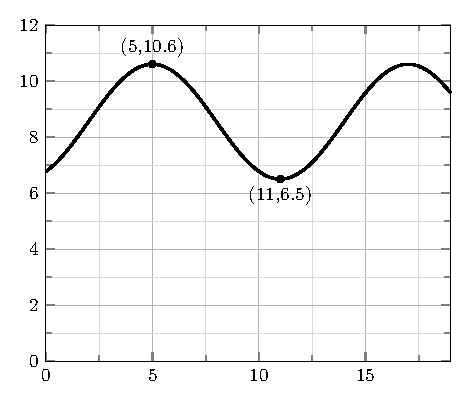
\includegraphics[width=.92\linewidth]{../figures/fhsm_2009_p52_1.pdf}
  \end{center}

  \item [Student 3:] Yeah, and if the highest and lowest the graph ever goes are $10.6$ meters and $6.5$ meters, then the amplitude is going to be $4.1$ meters, right? Oh, wait a minute---the amplitude is only half of the height, so we need to change that to $2.05$ meters.
  \item [Student 2:] OK, now once we know that, we can find out that the vertical shift is half way between the high and low points, which would make it $8.55$ meters.
  \item [Teacher:] Good job so far---now you just need to work on the period and horizontal shift. Do you think it would be easier to work with sine or cosine?
  \item [Student 1:] I like cosine better for this graph because we can see that a high point happens fi ve hours after midnight, so that will make it easy to find the horizontal shift.
\end{scriptlist}

The conversation could continue like this in small groups, followed by a whole-class discussion of the observations made by various groups. Students could check the reasonableness of their solutions by using a dynamic graphing utility. An interesting extension of this task would be to use the model to determine the times during which a ship with a certain depth requirement would be able to safely navigate into and out of the port.

\noindent
\textbf{Key Elements of Mathematics}

Reasoning with Functions---Modeling by using families of functions; Analyzing the effects of parameters

\noindent
\textbf{Reasoning Habits}

Analyzing a problem---applying previously learned concepts; making preliminary deductions and conjectures

Reflecting on a solution---considering the reasonableness of a solution
}
{Thủy triều}
{
\noindent
\textbf{Nhiệm vụ}

Thuyền trưởng của một con tàu phải tính đến thủy triều khi đưa tàu vào cảng biển, vì độ sâu của nước có thể thay đổi rất nhiều từ thời điểm này sang thời điểm khác trong ngày. Giả sử triều cao tại một cảng nào đó xảy ra vào lúc 5 giờ sáng, khi nước sâu $10.6$ mét, và lần triều thấp tiếp theo xảy ra vào lúc 11 giờ sáng, khi nước sâu $6.5$ mét. Hãy xây dựng một mô hình toán học dự đoán độ sâu của nước như một hàm của thời gian đã trôi qua kể từ nửa đêm.

\noindent
\textbf{Trong lớp học (Toán năm thứ tư)}

Lưu ý rằng các học sinh làm bài toán này đã có kinh nghiệm với các phép biến đổi của hàm bậc nhất và hàm bậc hai, đồng thời quen thuộc với đồ thị của các hàm sin và cos.

Sau đây là một ví dụ về cách học sinh luận về nhiệm vụ này:

\begin{scriptlist}
  \item [Giáo viên:] Ta mới chỉ được cho hai cặp có thứ tự, nên sẽ có nhiều kiểu đồ thị khác nhau có thể khớp với dữ liệu. Trong tình huống này, kiểu mô hình đại số nào là hợp lí?
  \item [Học sinh 1:] Hai điểm thì xác định một đường thẳng, đúng không ạ? Chẳng phải ta chỉ cần nối hai điểm đó lại sao?
  \item [Học sinh 2:] Không, mực nước không thể cứ giảm mãi như vậy được---nó sẽ lại dâng lên rồi lại hạ xuống mỗi ngày.
  \item [Học sinh 3:] Vậy thì có lẽ nó sẽ là một trong những đồ thị dạng sóng.
  \item [Học sinh 1:] À đúng rồi---em đoán nó sẽ là sin hoặc cos. Nhưng làm sao biết nên chọn cái nào?
  \item [Học sinh 3:] Thử vẽ một phần của làn sóng rồi xem ta có thể nhận ra điều gì.
  \item [Học sinh 2:] Nếu mẫu hình này lặp lại như thế sau mỗi sáu giờ, thì mỗi ngày sẽ có hai điểm cao và hai điểm thấp. Em đoán như vậy chu kì sẽ là $12$ giờ.

  \begin{center}
    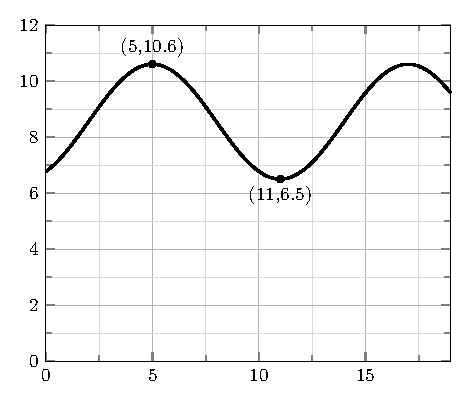
\includegraphics[width=.92\linewidth]{../figures/fhsm_2009_p52_1.pdf}
  \end{center}

  \item [Học sinh 3:] Đúng, và nếu giá trị lớn nhất và nhỏ nhất mà đồ thị đạt tới là $10.6$ mét và $6.5$ mét, thì biên độ sẽ là $4.1$ mét, đúng không? À, khoan đã---biên độ chỉ bằng một nửa độ cao đó thôi, nên phải đổi thành $2.05$ mét.
  \item [Học sinh 2:] Được rồi, giờ khi biết điều đó, ta có thể tìm được phép tịnh tiến theo phương thẳng đứng, là điểm nằm chính giữa mức cao và mức thấp, nên sẽ là $8.55$ mét.
  \item [Giáo viên:] Tốt lắm. Bây giờ các em chỉ còn phải xử lí chu kì và phép tịnh tiến theo phương ngang nữa thôi. Theo các em, dùng sin hay cos sẽ dễ hơn?
  \item [Học sinh 1:] Em thích dùng cos hơn cho đồ thị này vì ta thấy một điểm cao xuất hiện sau nửa đêm năm giờ, nên như vậy sẽ dễ tìm phép tịnh tiến theo phương ngang hơn.
\end{scriptlist}

Cuộc trao đổi có thể tiếp tục theo cách này trong các nhóm nhỏ, rồi sau đó là một cuộc thảo luận cả lớp về những nhận xét mà các nhóm khác nhau đã đưa ra. Học sinh có thể kiểm tra tính hợp lí của lời giải bằng cách dùng một công cụ vẽ đồ thị động. Một hướng mở rộng thú vị của nhiệm vụ này là dùng mô hình để xác định những khoảng thời gian mà một con tàu, với yêu cầu về độ sâu nhất định, có thể ra vào cảng một cách an toàn.

\noindent
\textbf{Các yếu tố then chốt của toán học}

Luận với hàm số---Mô hình hóa bằng các họ hàm số; Phân tích ảnh hưởng của các tham số

\noindent
\textbf{Các thói quen luận}

Phân tích bài toán---vận dụng các khái niệm đã học; đưa ra những suy diễn và phỏng đoán sơ bộ

Phản tư về lời giải---xem xét tính hợp lí của lời giải
}
{}

\TriPara
{
\EN{Opportunities to reason with functions and use them to model real-world situations arise at every stage of a high school student's mathematical development. Providing students with varied experiences involving functions can help them internalize the sometimes confusing mathematical language of function notation (Chazan and Yerushalmy 2003; Coulombe and Berenson 2001). The development of reasoning with functions is one of the cornerstones on which a well-developed understanding of mathematics is built.}
}
{
\VI{Cơ hội để luận với hàm số và dùng chúng nhằm mô hình hóa các tình huống trong thế giới thực xuất hiện ở mọi giai đoạn phát triển toán học của một học sinh trung học phổ thông. Việc tạo cho học sinh những trải nghiệm đa dạng với hàm số có thể giúp các em dần nội tại hóa thứ ngôn ngữ toán học đôi khi gây lúng túng của kí hiệu hàm số (Chazan and Yerushalmy 2003; Coulombe and Berenson 2001). Sự phát triển của luận với hàm số là một trong những nền tảng trụ cột để xây dựng nên một sự hiểu toán vững vàng.}
}
{
\NOTE{}
}

% ==========
% CHƯƠNG 7
% ==========

\ParallelChapter
  {Reasoning with Geometry}
  {Luận với hình học}
  {}

\TriPara
{
\EN{Classically, geometry has been the subject in which students encounter mathematical proof based on formal deduction. Although proof should be naturally incorporated in all areas of the curriculum, attention to proof in the geometry curriculum is strengthened by a focus on reasoning and sense making. In addition, geometry has connections with other mathematical domains and important applications in careers and in everyday life. Geometric ideas are a significant part of many high-technology developments, including high-definition television (HDTV), global positioning systems (GPS), computer animation, computerized axial tomography (CAT) scans, cellular telephone networks, robotics, virtual reality, and docking of the Space Shuttle. Geometric and visual reasoning often enter our daily lives.}
}
{
\VI{Theo truyền thống, hình học là lĩnh vực mà học sinh tiếp xúc với chứng minh toán học dựa trên suy diễn hình thức. Mặc dù chứng minh cần được tích hợp một cách tự nhiên trong tất cả các lĩnh vực của chương trình toán học, sự chú trọng đến chứng minh trong chương trình hình học được tăng cường khi đặt trọng tâm vào luận và hiểu. Bên cạnh đó, hình học có mối liên hệ với các lĩnh vực toán học khác và có những ứng dụng quan trọng trong nghề nghiệp cũng như trong đời sống hằng ngày. Các ý tưởng hình học là một bộ phận quan trọng của nhiều công nghệ cao, bao gồm truyền hình độ phân giải cao (HDTV), hệ thống định vị toàn cầu (GPS), hoạt hình máy tính, chụp cắt lớp vi tính (CAT), mạng điện thoại di động, robot, thực tế ảo và kỹ thuật ghép nối tàu con thoi. Luận hình học và trực quan thường xuyên xuất hiện trong đời sống hằng ngày của chúng ta.}
}
{
\NOTE{}
}

\TriPara
{
\EN{A considerable amount of research on students' thinking in geometry can be used to promote students' reasoning and sense making in this area. Much of this research bolsters the van Hiele levels of students' geometric thinking (Battista 2007). These five van Hiele levels of thinking are sequential and hierarchical, meaning that students must pass through lower levels if they are to attain higher levels. The van Hiele levels of students' thinking can be linked to the reasoning habits described in chapter 2 and can help promote students' attainment of the reasoning and sense-making abilities exemplified in this publication. For instance, the first two van Hiele levels, \emph{visual-holistic} and \emph{descriptive-analytic} reasoning, link to the \emph{empirical} reasoning level described in ``Progression of Reasoning'' in chapter 2. The third van Hiele level, \emph{relational-inferential} reasoning, connects with the \emph{preformal} level, and the fourth and fifth van Hiele levels, \emph{formal deductive proof} and \emph{rigor}, are tied to the \emph{formal} level of reasoning. Accordingly, knowledge about students' thinking not only allows us but requires us to support students at whatever level of thinking they may have attained when coming to high school and to provide them experiences that help them move to higher levels.}
}
{
\VI{Một lượng đáng kể các nghiên cứu về tư duy hình học của học sinh có thể được dùng để thúc đẩy luận và hiểu của học sinh trong lĩnh vực này. Phần lớn các nghiên cứu ấy củng cố quan niệm về các mức độ tư duy hình học của học sinh theo van Hiele (Battista 2007). Năm mức độ tư duy theo van Hiele này có tính tuần tự và thứ bậc, nghĩa là học sinh phải đi qua các mức thấp hơn nếu muốn đạt tới các mức cao hơn. Các mức độ tư duy của học sinh theo van Hiele có thể được liên kết với những thói quen luận được mô tả trong Chương 2, và có thể góp phần thúc đẩy việc học sinh đạt tới các năng lực luận và hiểu được minh họa trong công trình này. Chẳng hạn, hai mức độ đầu tiên theo van Hiele, \emph{luận trực quan-toàn thể} và \emph{luận mô tả-phân tích}, liên kết với mức độ luận \emph{thực nghiệm} được mô tả trong mục ``Tiến triển của luận'' ở Chương 2. Mức độ thứ ba theo van Hiele, \emph{luận quan hệ-suy luận}, tương ứng với mức \emph{tiền hình thức}, còn mức độ thứ tư và thứ năm, \emph{chứng minh suy diễn hình thức} và \emph{nghiêm ngặt}, gắn với mức độ luận \emph{hình thức}. Vì thế, hiểu biết về tư duy của học sinh không chỉ cho phép mà còn đòi hỏi ta phải hỗ trợ học sinh ở bất cứ mức độ tư duy nào mà các em đã đạt tới khi bước vào trung học phổ thông, đồng thời tạo cho các em những trải nghiệm giúp các em chuyển lên những mức độ cao hơn.}
}
{
\NOTE{Đoạn này đưa cơ sở nghiên cứu về tư duy hình học của học sinh vào trung tâm của định hướng dạy học. Điều tác giả muốn nhấn mạnh không chỉ là sự tồn tại của mô hình van Hiele, mà là hệ quả sư phạm của nó: sự phát triển tư duy hình học có tính tuần tự và thứ bậc, nên không thể đòi hỏi học sinh đạt tới chứng minh hình thức khi các em còn chưa đi qua những mức tư duy thấp hơn. Vì thế, nghiên cứu về tư duy của học sinh không phải một tri thức phụ trợ đứng ngoài lớp học, mà là căn cứ để quyết định nên yêu cầu gì và nên nâng đỡ học sinh theo hướng nào.

Điểm quan trọng hơn nữa là tác giả không dùng van Hiele như một lí thuyết riêng của hình học, tách biệt khỏi phần còn lại của cuốn sách. Các mức van Hiele được nối trực tiếp với tiến trình của luận đã trình bày ở Chương 2: hai mức đầu gắn với luận thực nghiệm, khi học sinh còn dựa nhiều vào quan sát và mô tả; mức thứ ba tương ứng với giai đoạn tiền hình thức, khi các quan hệ và suy ra bắt đầu hiện rõ; hai mức cao nhất gắn với luận hình thức, nơi chứng minh và tính chặt chẽ trở thành trung tâm. Nhờ cách nối này, hình học không hiện ra như một ngoại lệ trong sách, mà như một miền trong đó cùng một tiến trình phát triển của luận và hiểu được biểu hiện dưới một dạng đặc thù.

Câu kết của đoạn văn mang ý nghĩa sư phạm quyết định. Hiểu biết về tư duy của học sinh không chỉ cho phép mà còn buộc người dạy phải bắt đầu từ mức độ mà học sinh thực sự đang có, rồi tổ chức những trải nghiệm thích hợp để các em từng bước đi lên. Ở đây, tác giả đang bác bỏ ngầm một cách dạy quen thuộc: đòi hỏi quá sớm những hình thức suy diễn mà học sinh chưa có nền nhận thức để mang nổi. Đồng thời, đoạn này cũng biện minh cho giá trị của các hoạt động trực quan, mô tả và khám phá như những chặng cần thiết trên con đường đi tới chứng minh hình thức.}
}

\TriPara
{
\EN{Key elements of reasoning and sense making with geometry include the following:

\begin{itemize}
  \item \emph{Conjecturing about geometric objects.} Analyzing configurations and reasoning inductively about relationships to formulate conjectures.
  \item \emph{Construction and evaluation of geometric arguments.} Developing and evaluating deductive arguments (both formal and informal) about figures and their properties that help make sense of geometric situations.
  \item \emph{Multiple geometric approaches.} Analyzing mathematical situations by using transformations, synthetic approaches, and coordinate systems.
  \item \emph{Geometric connections and modeling.} Using geometric ideas, including spatial visualization, in other areas of mathematics, other disciplines, and in real-world situations.
\end{itemize}

We address these key elements in more detail in the following sections.}
}
{
\VI{Các yếu tố then chốt của luận và hiểu với hình học gồm có:

\begin{itemize}
  \item \emph{Phỏng đoán về các đối tượng hình học.} Phân tích các cấu hình và luận quy nạp về các quan hệ để hình thành các phỏng đoán.
  \item \emph{Xây dựng và thẩm định các lập luận hình học.} Phát triển và thẩm định các lập luận suy diễn, cả hình thức lẫn không hình thức, về các hình và các tính chất của chúng nhằm giúp hiểu các tình huống hình học.
  \item \emph{Nhiều cách tiếp cận hình học.} Phân tích các tình huống toán học bằng cách sử dụng các phép biến hình, các cách tiếp cận tổng hợp, và các hệ tọa độ.
  \item \emph{Các kết nối hình học và mô hình hóa.} Sử dụng các ý tưởng hình học, bao gồm hình dung không gian, trong những lĩnh vực khác của toán học, trong các môn học khác, và trong những tình huống thực tế.
\end{itemize}

Chúng tôi sẽ trình bày chi tiết hơn các yếu tố then chốt này trong các phần tiếp theo.}
}
{
\NOTE{}
}

\ParallelSection
  {Conjecturing about Geometric Objects}
  {Phỏng đoán về các đối tượng hình học}
  {}


\TriPara
{
\EN{Making conjectures is a fundamental reasoning habit in mathematical inquiry. Geometry offers many opportunities for developing this reasoning habit through an abundance of intriguing and often surprising visual or measurable geometric relationships. Students can make conjectures by analyzing a planar or spatial configuration or by wondering whether a certain configuration can exist. Conjecturing activates their natural inquisitiveness, not only about “what might be happening” (the conjecture) but ``why it would be happening'' (looking for insight, validation, or refutation.) The process of seeking and making conjectures gives students the opportunity to become immersed in, and deepen their understanding of, the mathematical relationships involved, as well to sharpen their ability to validate them. By making conjectures about novel situations, students also learn to employ mathematics in new situations, a highly desirable skill in our fast-changing world. Further mention of this skill is made in the section titled ``Geometric connections and modeling.''}
}
{
\VI{Việc đưa ra phỏng đoán là một thói quen luận nền tảng trong hoạt động tìm tòi toán học. Hình học mang lại nhiều cơ hội để phát triển thói quen luận này thông qua vô số các mối quan hệ hình học trực quan hoặc có thể đo đạc được, thường gây hứng thú và đôi khi bất ngờ. Học sinh có thể đưa ra các phỏng đoán bằng cách phân tích một cấu hình phẳng hoặc không gian, hoặc bằng cách tự hỏi liệu một cấu hình nhất định có thể tồn tại hay không. Hoạt động phỏng đoán khơi dậy tính tò mò tự nhiên của học sinh, không chỉ về ``điều gì có thể đang diễn ra'' (bản thân phỏng đoán), mà còn về ``vì sao điều đó lại xảy ra'' (tìm kiếm sự hiểu biết sâu sắc, sự xác nhận hoặc sự bác bỏ). Quá trình tìm kiếm và hình thành các phỏng đoán tạo cơ hội để học sinh đắm mình vào các mối quan hệ toán học liên quan, qua đó làm sâu sắc thêm sự hiểu biết của các em, đồng thời rèn luyện khả năng kiểm chứng các mối quan hệ đó. Thông qua việc đưa ra các phỏng đoán trong những tình huống mới mẻ, học sinh còn học cách vận dụng toán học trong những bối cảnh mới, một kỹ năng đặc biệt cần thiết trong một thế giới đang thay đổi nhanh chóng. Kỹ năng này sẽ tiếp tục được đề cập trong mục có tiêu đề ``Các kết nối hình học và mô hình hóa bằng hình học''.}
}
{
\NOTE{}
}

\TriPara
{
\EN{In example 14 students develop mathematical conjectures related to a context drawn from everyday life. In addition to the immediate utility of the results in the context itself, such contexts (1) provide a recognizable, interesting situation in which students can immerse themselves for the purpose of mathematical analysis, (2) offer multiple accessible methods to explore the situation for the purpose of creating conjectures, and (3) foster the notion that mathematics is everywhere. Example 15, ``Circling the Points,'' builds on example 14. These two examples would appear in the curriculum after students have studied some properties of perpendicularity (e.g., that a point lies on the perpendicular bisector of a line segment if and only if it is equidistant from the two endpoints of the segment.) They would appear early in the study of geometric properties of circles and would ultimately lead to the study of the inscribed angle theorem and related results. These examples also support the reasoning habits of making conjectures and using deduction to explore those conjectures.}
}
{
\VI{Trong Ví dụ 14, học sinh xây dựng những phỏng đoán toán học gắn với một bối cảnh lấy từ đời sống hằng ngày. Ngoài tính hữu ích trực tiếp của các kết quả ngay trong chính bối cảnh ấy, những bối cảnh như vậy còn có ba giá trị khác: (1) cung cấp một tình huống quen thuộc, thú vị để học sinh có thể thực sự dấn mình vào đó cho mục đích phân tích toán học; (2) mở ra nhiều cách tiếp cận dễ tiếp cận để khảo sát tình huống nhằm hình thành các phỏng đoán; và (3) nuôi dưỡng ý niệm rằng toán học hiện diện ở khắp nơi. Ví dụ 15, ``Tâm ở đâu?'', được xây dựng tiếp nối từ Ví dụ 14. Hai ví dụ này sẽ xuất hiện trong chương trình sau khi học sinh đã học một số tính chất của sự vuông góc, chẳng hạn tính chất: một điểm nằm trên đường trung trực của một đoạn thẳng khi và chỉ khi nó cách đều hai đầu mút của đoạn thẳng ấy. Chúng sẽ được đưa vào ở giai đoạn đầu của việc học các tính chất hình học của đường tròn, và sau cùng sẽ dẫn tới việc học định lí góc nội tiếp cùng các kết quả liên quan. Hai ví dụ này cũng hỗ trợ các thói quen luận như hình thành phỏng đoán và dùng suy diễn để khảo sát các phỏng đoán ấy.}
}
{
\NOTE{}
}

\TriExample
{Picture This}
{
\noindent
\textbf{Task}

In photography, the ``horizontal viewing angle'' describes the angular extent of a scene being captured, with the vertex representing the camera lens. (See the figure at the right, which depicts the horizontal plane of the camera shot.)

\begin{center}
  \includegraphics[width=.92\linewidth]{../figures/fhsm_2009_p56_1.pdf}
\end{center}

Shelly wants to take an artistic photo of the decorated side of a building that sits on a flat plot of land. She wants to capture a level shot of the full width of the building (exactly), but she does not care whether the full building height is in the picture. So the horizontal expanse of the picture is fixed.

She is using a camera lens with a fixed horizontal viewing angle of 50 degrees, and she wants to take a level shot of the side of the building. She has found one spot that works, as indicated by point P in the figure at the right. Shelly believes that she could stand at other places to capture the same horizontal expanse but from a different perspective. Before she snaps the picture, she wants to examine some of those other positions. Your task is to figure out the ground locations where Shelly could stand to create a picture fitting her criteria.

\begin{center}
  \includegraphics[width=.92\linewidth]{../figures/fhsm_2009_p57_1.pdf}
\end{center}

Explore the situation, write down any conjectures you have regarding possible positions, and justify any that you can. The objective is to eventually create a conjecture describing the full range of possible positions. Prepare to clearly state your conjectures, as well as the thinking, exploration, and reasoning that explain how you arrived at them.

\noindent
\textbf{In the Classroom (Geometry Class)}

An interactive drawing utility (with a file containing the sketch above), a hard copy of the sketch and a physical manipulative (a rigid angle---e.g., the expanse of a rigid compass), or a real camera and wall could be used to facilitate exploration of possible locations. The lesson begins with a full-class discussion of initial thoughts. After some time for individual thought or explanation, the following dialogue ensues.

\begin{scriptlist}
  \item [Teacher:] Do you have any immediate conjectures to suggest?
  \item [Student 1:] I think there is a point right in the middle where you could stand.
  \item [Teacher:] What do you mean by ``middle''?
  \item [Student 1:] I mean I would stand at a point in the diagram that would be the same distance from points $A$ and $B$.
  \item [Student 2:] Oh, that means the point would be somewhere on the perpendicular bisector of the segment $AB$, which represents the building side. This is because we have already learned that the perpendicular bisector of the segment is the collection of points that are equidistant from points $A$ and $B$.
  \item [Teacher:] How would you find such a point? The students engage in some more work.
  \item [Student 1:] I'd put a point on the perpendicular bisector of segment $AB$ and then move it back and forth until the angle exactly fit the segment.
  \item [Teacher:] Good, that gives some detail regarding how one might locate a second point. [The teacher writes down a conjecture that there is a possible vertex location on the perpendicular bisector of segment $AB$. This conjecture will be addressed in a subsequent discussion---beyond the confines of this example.] Are there other ideas about possible vertices?
    
  \begin{center}
    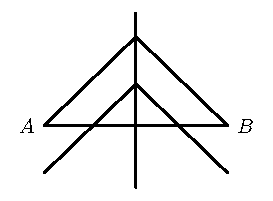
\includegraphics[width=.92\linewidth]{../figures/fhsm_2009_p57_2.pdf}
  \end{center}

  \item [Student 2:] Based on my experience with a camera, I think there would be many points where one could stand to show the entire building side.
\end{scriptlist}

Many students in the class agree with the conjecture that many points would work. Another student jumps in and suggests that that the possible positions possess symmetry. Eventually, someone states that reflective symmetry would be evident in the collection of possible points across the perpendicular bisector of $AB$. This conjecture will be evaluated subsequently, as well.

\begin{scriptlist}
  \item [Teacher:] Now, by using either the interactive drawing utility or the physical manipulative, plot a collection of points that represent where the photographer might stand to snap the required image. See if any other conjectures emerge from this exploration.
  \item [Student 4:] [After some exploration] All the points seem to be on a circular arc that goes from point $A$ to point $B$---even though the photographer can't stand there.
  
  \begin{center}
    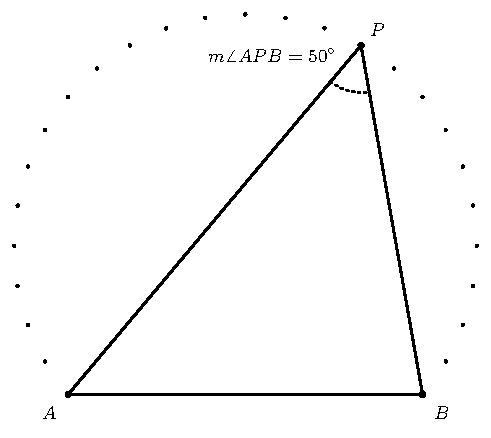
\includegraphics[width=.92\linewidth]{../figures/fhsm_2009_p58_1.pdf}
  \end{center}
\end{scriptlist}

The teacher next facilitates a discussion about stating in abstract terms what we refer to as the major conjecture: ``Given a line segment $AB$ and a specified side of line $AB$, each point, $P$, on the specified side of $AB$ with the property that $m\angle APB = 50^\circ$ lies on a circular arc containing $A$ and $B$.''

This conjecture is not resolved immediately. Rather, a set of questions is compiled by the class for moving toward a proof of this conjecture. These questions include the following:

\begin{enumerate}
  \item Can we find out which circular arc we are talking about? That is, can we find the circle that contains this arc?
  \item Would every point on the arc (except points $A$ and $B$) represent possible positions where the photographer could stand?
  \item Would the arc miss any possible points?
\end{enumerate}

(See example 15 along with the supporting topic book on geometry for a full discussion of the conjecture.)

\noindent
\textbf{Key Elements of Mathematics}

Reasoning with Geometry---Conjecturing about geometric objects; Multiple geometric approaches

\noindent
\textbf{Reasoning Habits}

Analyzing the problem---identifying relevant concepts, representations, or procedures; looking for hidden structure; considering special cases or simpler analogs; seeking patterns and relationships; making preliminary deductions and conjectures 

Implementing a strategy-monitoring progress toward a solution; making logical deductions
}
{Đứng đâu để chụp?}
{
\noindent
\textbf{Task}

Trong nhiếp ảnh,``góc nhìn ngang'' mô tả độ mở góc của cảnh được thu vào ảnh, với đỉnh góc là ống kính máy ảnh. (Xem hình bên dưới, biểu diễn mặt phẳng ngang của cảnh chụp.)

\begin{center}
  \includegraphics[width=.92\linewidth]{../figures/fhsm_2009_p56_1.pdf}
\end{center}

Shelly muốn chụp một bức ảnh nghệ thuật mặt được trang trí của một tòa nhà nằm trên một khu đất bằng phẳng. Cô muốn chụp một bức ảnh ngang sao cho toàn bộ bề rộng của tòa nhà được thu vào khung hình (một cách chính xác), nhưng không quan tâm liệu toàn bộ chiều cao của tòa nhà có xuất hiện trong ảnh hay không. Do đó, độ mở ngang của bức ảnh là cố định.

Cô đang sử dụng một ống kính có góc nhìn ngang cố định là $50$ độ và muốn chụp một bức ảnh ngang của mặt bên tòa nhà. Cô đã tìm được một vị trí phù hợp, được ký hiệu là điểm $P$ trong hình bên dưới. Shelly tin rằng cô có thể đứng ở những vị trí khác để chụp được cùng một độ mở ngang đó nhưng từ những góc nhìn khác nhau. Trước khi bấm máy, cô muốn xem xét một số vị trí khác như vậy. Nhiệm vụ của bạn là xác định các vị trí trên mặt đất mà Shelly có thể đứng để tạo ra một bức ảnh thỏa mãn các tiêu chí đã nêu.

\begin{center}
  \includegraphics[width=.92\linewidth]{../figures/fhsm_2009_p57_1.pdf}
\end{center}

EHãy khám phá tình huống này, ghi lại bất kỳ phỏng đoán nào bạn có liên quan đến các vị trí có thể có, và biện minh cho những phỏng đoán mà bạn có thể. Mục tiêu cuối cùng là hình thành một phỏng đoán mô tả đầy đủ tập hợp các vị trí có thể. Hãy chuẩn bị để trình bày rõ ràng các phỏng đoán của bạn, cũng như các suy nghĩ, quá trình khám phá và lập luận đã dẫn bạn tới chúng.

\noindent
\textbf{Trong lớp học (Lớp Hình học)}

Một công cụ vẽ tương tác (với tệp chứa hình phác thảo như trên), một bản in của hình vẽ và một dụng cụ thao tác vật lý (một góc cứng---chẳng hạn độ mở của một compa cố định), hoặc một máy ảnh thật và một bức tường, đều có thể được sử dụng để hỗ trợ việc khám phá các vị trí có thể. Bài học bắt đầu bằng một cuộc thảo luận chung của cả lớp về những suy nghĩ ban đầu. Sau một khoảng thời gian để suy nghĩ hoặc giải thích cá nhân, cuộc đối thoại sau đây diễn ra.

\begin{scriptlist}
  \item [Giáo viên:] Các em có phỏng đoán ban đầu nào muốn đề xuất không?
  \item [Học sinh 1:] Em nghĩ có một điểm ở ngay chính giữa nơi người ta có thể đứng.
  \item [Giáo viên:] Em có ý gì khi nói ``chính giữa''?
  \item [Học sinh 1:] Em muốn nói là em sẽ đứng tại một điểm trong hình sao cho khoảng cách đến các điểm $A$ và $B$ là như nhau.
  \item [Học sinh 2:] OÀ, như vậy có nghĩa là điểm đó nằm đâu đó trên đường trung trực của đoạn thẳng $AB$, đoạn thẳng biểu diễn mặt bên của tòa nhà. Điều này là vì chúng em đã học rằng đường trung trực của một đoạn thẳng là tập hợp các điểm cách đều hai đầu mút của đoạn thẳng đó.
  \item [Giáo viên:] Em sẽ tìm một điểm như vậy bằng cách nào? Học sinh tiếp tục làm việc thêm một lúc.
  \item [Học sinh 1:] Em sẽ đặt một điểm trên đường trung trực của đoạn $AB$ rồi di chuyển nó tới lui cho đến khi góc vừa khít với đoạn thẳng.
  \item [Giáo viên:] Tốt, điều đó cho thấy khá rõ cách người ta có thể xác định một điểm thứ hai. [Giáo viên ghi lại một phỏng đoán rằng có một vị trí đỉnh có thể nằm trên đường trung trực của đoạn $AB$. Phỏng đoán này sẽ được xem xét trong một thảo luận tiếp theo---vượt ra ngoài phạm vi của ví dụ này.] Có ý tưởng nào khác về các vị trí đỉnh có thể có không?
    
  \begin{center}
    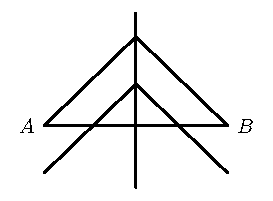
\includegraphics[width=.92\linewidth]{../figures/fhsm_2009_p57_2.pdf}
  \end{center}

  \item [Học sinh 2:] Dựa trên kinh nghiệm của em với máy ảnh, em nghĩ sẽ có rất nhiều điểm mà người ta có thể đứng để chụp trọn mặt bên của tòa nhà.
\end{scriptlist}

Nhiều học sinh trong lớp đồng ý với phỏng đoán rằng có rất nhiều điểm phù hợp. Một học sinh khác tham gia và gợi ý rằng các vị trí có thể có mang tính đối xứng. Cuối cùng, có người cho rằng đối xứng qua trục sẽ xuất hiện trong tập hợp các điểm có thể có, đối xứng qua đường trung trực của $AB$. Phỏng đoán này cũng sẽ được đánh giá sau đó.

\begin{scriptlist}
  \item [Giáo viên:]Bây giờ, bằng cách sử dụng công cụ vẽ tương tác hoặc dụng cụ thao tác vật lý, hãy vẽ một tập hợp các điểm biểu diễn những vị trí mà nhiếp ảnh gia có thể đứng để chụp bức ảnh theo yêu cầu. Hãy xem liệu có phỏng đoán nào khác xuất hiện từ quá trình khám phá này không.
  \item [Học sinh 4:]  [Sau một thời gian khám phá] Tất cả các điểm dường như đều nằm trên một cung tròn đi từ điểm $A$ đến điểm $B$---mặc dù nhiếp ảnh gia không thể đứng tại các điểm đó.
  
  \begin{center}
    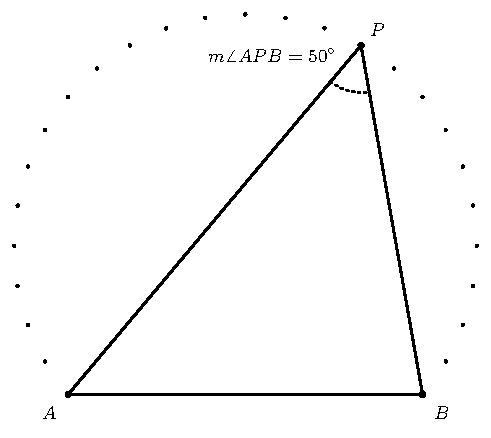
\includegraphics[width=.92\linewidth]{../figures/fhsm_2009_p58_1.pdf}
  \end{center}
\end{scriptlist}

Sau đó, giáo viên điều phối một cuộc thảo luận về việc phát biểu một cách trừu tượng điều mà ta gọi là phỏng đoán chính: ``Cho một đoạn thẳng $AB$ và một phía xác định của đường thẳng $AB$, mỗi điểm $P$ nằm về phía đã xác định của $AB$ thỏa mãn điều kiện $m\angle APB = 50^\circ$ đều nằm trên một cung tròn chứa $A$ và $B$.''

Phỏng đoán này không được giải quyết ngay lập tức. Thay vào đó, lớp học tổng hợp một tập hợp các câu hỏi nhằm tiến tới việc chứng minh phỏng đoán này. Các câu hỏi đó bao gồm:

\begin{enumerate}
  \item Chúng ta có thể xác định được cung tròn nào đang được nói tới không? Nói cách khác, ta có thể tìm được đường tròn chứa cung đó hay không?
  \item Mọi điểm trên cung (trừ các điểm $A$ và $B$) có đều biểu diễn các vị trí mà nhiếp ảnh gia có thể đứng hay không?
  \item Liệu cung tròn đó có bỏ sót vị trí khả dĩ nào không?
\end{enumerate}

(Xem Ví dụ 15 cùng với tài liệu chủ đề hỗ trợ về hình học để có một thảo luận đầy đủ về phỏng đoán này.)

\noindent
\textbf{Các yếu tố then chốt của toán học}

Luận với hình học---Phỏng đoán về các đối tượng hình học; Nhiều cách tiếp cận hình học

\noindent
\textbf{Các thói quen luận}

Phân tích bài toán---xác định các khái niệm, thủ tục, hoặc biểu diễn toán học thích đáng; tìm kiếm cấu trúc ẩn; xét các trường hợp đặc biệt hoặc những trường hợp tương tự đơn giản hơn; tìm kiếm các mẫu hình và quan hệ; đưa ra những suy diễn và phỏng đoán sơ bộ

Triển khai chiến lược---theo dõi tiến trình đi đến lời giải; thực hiện những suy diễn có tính luận lý
}
{}

\ParallelSection
  {Construction and Evaluation of Geometric Arguments}
  {Xây dựng và thẩm định các biện giải hình học}
  {}

\TriPara
{
\EN{Making a conjecture, as in example 14, is a first step in mathematical inquiry. Students need to follow up many of their conjectures with efforts to either justify or disprove them. Although the major conjecture in example 14 is not resolved immediately, the activity leads naturally to the development of several important geometric results that emerge from question 1 in the example. In particular, the students in example 15 make progress toward resolving the conjecture by establishing the fact that three noncollinear points in the plane lie on a unique circle. Further progress is made when students prove the inscribed angle theorem, which states that every point, $P$, on the conjectured circular arc would satisfy the condition that $m\angle APB$ equals 50 degrees. However, students would still need to prove that no other point on the same side of line AB could be the vertex of such an angle. Example 15 also exemplifies the reasoning habit of looking for hidden structure---in this example, an auxiliary line.}
}
{
\VI{Việc đưa ra một phỏng đoán, như trong Ví dụ 14, là bước khởi đầu của quá trình tìm tòi toán học. Học sinh cần tiếp tục theo đuổi nhiều phỏng đoán của mình bằng những nỗ lực nhằm biện minh hoặc bác bỏ chúng. Mặc dù phỏng đoán chính trong Ví dụ 14 không được giải quyết ngay lập tức, hoạt động này dẫn dắt một cách tự nhiên tới việc hình thành một số kết quả hình học quan trọng, xuất phát từ câu hỏi thứ nhất trong ví dụ. Cụ thể, trong Ví dụ 15, học sinh tiến thêm một bước trong việc giải quyết phỏng đoán bằng cách xác lập thực tế rằng ba điểm không thẳng hàng trong mặt phẳng cùng nằm trên một đường tròn duy nhất. Những tiến triển tiếp theo đạt được khi học sinh chứng minh định lý góc nội tiếp, theo đó mọi điểm $P$ nằm trên cung tròn được phỏng đoán đều thỏa mãn điều kiện $m\angle APB$ bằng $50$ độ. Tuy nhiên, học sinh vẫn cần phải chứng minh rằng không tồn tại điểm nào khác, nằm về cùng một phía của đường thẳng $AB$, có thể là đỉnh của một góc như vậy. Ví dụ 15 cũng minh họa một thói quen luận quan trọng, đó là tìm kiếm cấu trúc ẩn---trong trường hợp này, là việc bổ sung một đường phụ trợ.}
}
{
\NOTE{}
}

\TriPara
{
\EN{The progress in levels of reasoning can clearly be seen in these two examples. Students begin with explorations at the empirical level, moving to the preformal level as students suggest initial conclusions that can be drawn, such as that the arc actually passes through endpoints $A$ and $B$. Example 15 picks up the discussion with increasingly formal reasoning, culminating in conclusions supported by formal proof.}
}
{
\VI{Sự tiến triển qua các mức độ luận được thể hiện rõ ràng trong hai ví dụ này. Học sinh khởi đầu bằng các hoạt động khám phá ở mức thực nghiệm, rồi chuyển sang mức tiền hình thức khi các em đề xuất những kết luận ban đầu có thể rút ra, chẳng hạn như việc cung tròn thực sự đi qua hai đầu mút $A$ và $B$. Ví dụ 15 tiếp nối cuộc thảo luận với các hình thức luận ngày càng mang tính hình thức hơn, và đạt tới đỉnh điểm là những kết luận được nâng đỡ bằng chứng minh hình thức.}
}
{
\NOTE{}
}


\TriExample
{Circle of Points}
{
\noindent
\textbf{Task}

This task answers question 1 raised at the end of example 14, “Picture This”: What circle contains the conjectured arc?

  \begin{center}
    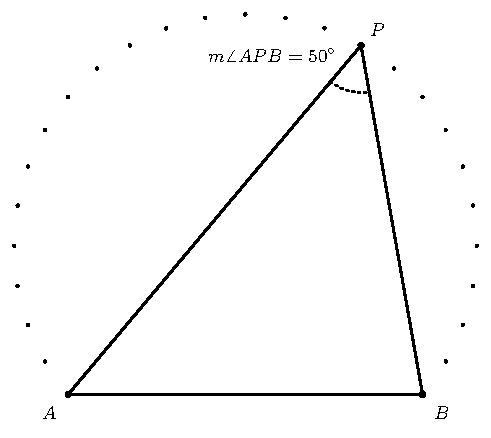
\includegraphics[width=.92\linewidth]{../figures/fhsm_2009_p58_1.pdf}
  \end{center}

\noindent
\textbf{In the Classroom (Geometry Class)}

Students are divided into groups with the assignment to decide what to do next. After a short time, the groups report on possible strategies:

\begin{scriptlist}
  \item [Group 1:] We think you need to find the center and radius of the circle.
  \item [Group 2:] We think you just need to find the center of the circle. You don't need to find the radius, because you already know at least one point on the circle---either the point $P$ specified in the original problem or points $A$ or $B$, which are part of the conjecture. You can use the center and one of these points on the circle to draw the whole circle.
  \item [Group 3:] We think you need the center. We think the center should be a point on segment $AB$ halfway between $A$ and $B$. The radius should be half the length of segment $AB$.
\end{scriptlist}

The groups reconvene to discuss these and possibly other thoughts. After a few more minutes the groups report.

\begin{scriptlist}
  \item [Group 4:] We tested to see if the midpoint of segment $AB$ would be the center. The circle did not go through the point $P$ we were given, so the midpoint is not the center in this case. So next we used the interactive drawing utility to try to create the circle that fit the points and figure out its center. We got a pretty good circle. We didn't think it would fit all the points because we just approximated the locations of points that would be vertices of 50 degree angles when we made them. But we are even more convinced that there is a circle through the point $P$, which we were using for the 50 degree angle, and points $A$ and $B$---and all actual real points where the photographer could stand.
  
    \begin{center}
      \includegraphics[width=.92\linewidth]{../figures/fhsm_2009_p60_1.pdf}
    \end{center}

  We then tried to think about the center and agreed that the center (like the midpoint of segment $AB$) needs to be equidistant from both $A$ and $B$, since the circle goes through $A$ and $B$. Thinking back to what we talked about when we started example 14, we conclude that the center of the circle has to be on the perpendicular bisector of segment $AB$. We added the perpendicular bisector of segment $AB$ to our drawing, and it went right through the center of the circle we had drawn---just like it was supposed to!

  Then someone else in our group noticed that the same reasoning works with the two points $A$ and $P$. That is, since the circle goes through $A$ and $P$, its center would have to lie on the perpendicular bisector of the segment $AP$, as well. We added the perpendicular bisector of segment $AP$ to our sketch, constructed these two bisectors, and found that they intersect in one point, which we called $G$. That is the only point that lies on both perpendicular bisectors.

  So it is the only possible point for the center of a circle. So we could now draw the circle by choosing the center and any one of the points $A$, $P$, or $B$.

  \item [Teacher:] Before you draw your circle, let me ask you a question. It seems that you have shown that if there is a circle through the points $P$, $A$, and $B$, the center must be $G$. Can you or any other group prove that there will definitely be such a circle---that you weren't just lucky this time with these particular points or that the drawing is misleading? Let's work on that in our groups.  
\end{scriptlist}

After a few minutes, a new group is ready to contribute its proof:

\begin{scriptlist}
  \item [Group 5:] We are assuming that we have the three noncollinear points $P$, $A$, and $B$ and that $G$ is the point of intersection of the perpendicular bisectors of sides $AB$ and $AP$-like we have been talking about. We will show that $G$ is the center of a circle that goes through points $P$, $A$, and $B$. Construct segments $GP$, $GA$, and $GB$. Segments $GP$ and $GA$ have to have equal lengths because $G$ is on the perpendicular bisector of segment $AP$. Segments $GA$ and $GB$ must be equal in length because $G$ is on the perpendicular bisector of segment $AB$. Since both segments $GP$ and $GB$ are equal in length to segment $GA$, all three segments have equal length. So if we draw the circle with center $G$ and radius equal to the length of segment $GA$, the circle will defi nitely go through the three points $A$, $B$, and $P$.

  \begin{center}
    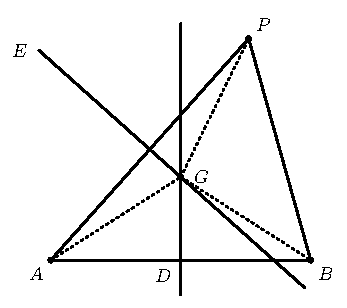
\includegraphics[width=.92\linewidth]{../figures/fhsm_2009_p61_1.pdf}
  \end{center}
\end{scriptlist}

The teacher asks for comments and critiques from the class with regard to group 5's presentation. (There are none.) The teacher then proposes that the day's discussion suggests three results: (1) Three noncollinear points in the plane determine a unique circle. (2) (Circle construction algorithm) The center of that circle can be found by finding the point of intersection of the perpendicular bisectors of any two sides of the triangle that has the three noncollinear points as vertices. (3) The perpendicular bisectors of the three sides of a triangle intersect in a single point. The first two of these results comes directly from the discussion. The third is closely related.

For homework, students are asked to write proofs of the first and third statements. In some instances this assignment requires organization, generalization, or extension of arguments given in the discussion. In others it involves adding detail. For the second statement, the students are asked to write an algorithm (i.e., well-defined sequence of steps) for constructing a circle through three noncollinear points in the plane.

\noindent
\textbf{Key Elements}

Reasoning with Geometry---Construction and evaluation of geometric arguments

\noindent
\textbf{Reasoning Habits}

Analyzing a problem---identifying relevant mathematical concepts, representations, or procedures; looking for hidden structure

Implementing a strategy ---- organizing a solution; making logical deductions; monitoring progress toward a solution

Reflecting on a solution ---- justifying or validating a solution
}
{Tâm ở đâu?}
{
\noindent
\textbf{Task}

Nhiệm vụ này trả lời câu hỏi 1 được nêu ra ở cuối Ví dụ 14, ``Đứng đâu để chụp?'': Đường tròn nào chứa cung tròn được phỏng đoán?

  \begin{center}
    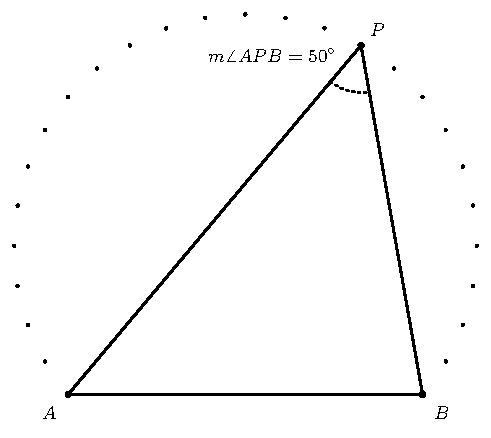
\includegraphics[width=.92\linewidth]{../figures/fhsm_2009_p58_1.pdf}
  \end{center}

\noindent
\textbf{rong lớp học (Lớp Hình học)}

Học sinh được chia thành các nhóm và được giao nhiệm vụ quyết định bước tiếp theo cần thực hiện. Sau một thời gian ngắn, các nhóm báo cáo về những chiến lược có thể có:

\begin{scriptlist}
  \item [Nhóm 1:] Chúng em nghĩ cần tìm tâm và bán kính của đường tròn.
  \item [Nhóm 2:] Chúng em nghĩ chỉ cần tìm tâm của đường tròn. Không cần tìm bán kính, vì ta đã biết ít nhất một điểm nằm trên đường tròn---hoặc điểm $P$ được cho trong bài toán ban đầu, hoặc các điểm $A$ hay $B$, vốn là một phần của phỏng đoán. Có thể dùng tâm và một trong những điểm ấy trên đường tròn để vẽ toàn bộ đường tròn.
  \item [Nhóm 3:] Chúng em nghĩ rằng cần tìm tâm. Theo chúng em, tâm phải là điểm nằm trên đoạn $AB$, ở chính giữa $A$ và $B$. Bán kính sẽ bằng một nửa độ dài đoạn $AB$.
\end{scriptlist}

ác nhóm tập hợp lại để thảo luận về những ý tưởng này, cũng như những suy nghĩ khác có thể có. Sau vài phút nữa, các nhóm tiếp tục báo cáo.

\begin{scriptlist}
  \item [Nhóm 4:] Chúng em kiểm tra xem trung điểm của đoạn $AB$ có phải là tâm không. Đường tròn không đi qua điểm $P$ đã cho, nên trong trường hợp này trung điểm không phải là tâm. Vì vậy, tiếp theo chúng em dùng công cụ vẽ tương tác để thử dựng đường tròn đi qua các điểm đã cho và tìm tâm của nó. Chúng em dựng được một đường tròn khá tốt. Ban đầu chúng em không nghĩ nó sẽ đi qua tất cả các điểm, vì khi tạo các điểm ấy chúng em chỉ ước lượng vị trí của những điểm sẽ là đỉnh của các góc $50^\circ$. Nhưng giờ chúng em còn tin hơn rằng có một đường tròn đi qua điểm $P$, là điểm mà chúng em dùng cho góc $50^\circ$, và qua các điểm $A$ và $B$---cũng như qua mọi điểm thực sự mà người chụp ảnh có thể đứng.
  
    \begin{center}
      \includegraphics[width=.92\linewidth]{../figures/fhsm_2009_p60_1.pdf}
    \end{center}

  Sau đó, chúng em nghĩ tiếp về tâm và đồng ý rằng tâm, cũng như trung điểm của đoạn $AB$, phải cách đều $A$ và $B$, vì đường tròn đi qua $A$ và $B$. Nhớ lại điều đã bàn khi bắt đầu Ví dụ 14, chúng em kết luận rằng tâm của đường tròn phải nằm trên đường trung trực của đoạn $AB$. Chúng em thêm đường trung trực của đoạn $AB$ vào hình vẽ, và nó đi đúng qua tâm của đường tròn mà chúng em đã dựng---đúng như dự đoán!

  Rồi một bạn khác trong nhóm nhận ra rằng cách lập luận ấy cũng đúng với hai điểm $A$ và $P$. Nghĩa là, vì đường tròn đi qua $A$ và $P$, nên tâm của nó cũng phải nằm trên đường trung trực của đoạn $AP$. Chúng em thêm đường trung trực của đoạn $AP$ vào hình phác, dựng hai đường trung trực ấy, và thấy chúng cắt nhau tại một điểm, chúng em gọi là $G$. Đó là điểm duy nhất nằm trên cả hai đường trung trực.

  Vì thế, đó là điểm duy nhất có thể là tâm của một đường tròn. Do đó, bây giờ chúng em có thể vẽ đường tròn bằng cách chọn tâm và một trong ba điểm $A$, $P$, hoặc $B$.

  \item [Giáo viên:] Trước khi các em vẽ đường tròn, thầy muốn hỏi một câu. Có vẻ như các em đã chỉ ra rằng nếu có một đường tròn đi qua các điểm $P$, $A$, và $B$, thì tâm của nó phải là $G$. Các em, hoặc nhóm nào khác, có thể chứng minh rằng chắc chắn sẽ có một đường tròn như vậy không---rằng không phải lần này các em chỉ tình cờ gặp may với những điểm cụ thể này, hay hình vẽ đang đánh lừa ta? Hãy tiếp tục làm việc trong nhóm về điều đó.
\end{scriptlist}

After a few minutes, a new group is ready to contribute its proof:

\begin{scriptlist}
  \item [Nhóm 5:] Chúng em giả sử có ba điểm không thẳng hàng $P$, $A$ và $B$, và $G$ là giao điểm của các đường trung trực của các đoạn $AB$ và $AP$, như chúng ta đang thảo luận. Chúng em sẽ chỉ ra rằng $G$ là tâm của một đường tròn đi qua các điểm $P$, $A$ và $B$. Hãy dựng các đoạn $GP$, $GA$ và $GB$. Các đoạn $GP$ và $GA$ phải có độ dài bằng nhau vì $G$ nằm trên đường trung trực của đoạn $AP$. Các đoạn $GA$ và $GB$ cũng phải bằng nhau vì $G$ nằm trên đường trung trực của đoạn $AB$. Vì cả hai đoạn $GP$ và $GB$ đều có độ dài bằng độ dài đoạn $GA$, nên cả ba đoạn này đều bằng nhau. Do đó, nếu vẽ đường tròn có tâm $G$ và bán kính bằng độ dài đoạn $GA$, thì đường tròn chắc chắn sẽ đi qua ba điểm $A$, $B$ và $P$.

  \begin{center}
    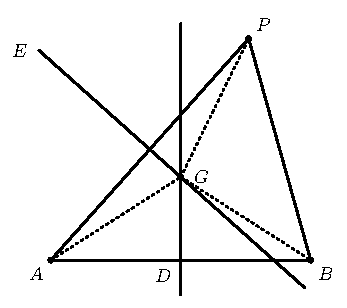
\includegraphics[width=.92\linewidth]{../figures/fhsm_2009_p61_1.pdf}
  \end{center}
\end{scriptlist}

  Giáo viên yêu cầu cả lớp nhận xét và phản biện phần trình bày của Nhóm 5. (Không có ý kiến nào.) Sau đó, giáo viên đề xuất rằng cuộc thảo luận trong ngày gợi ra ba kết quả: (1) Ba điểm không thẳng hàng trong mặt phẳng xác định một đường tròn duy nhất. (2) (Thuật toán dựng đường tròn) Tâm của đường tròn ấy có thể được tìm bằng cách xác định giao điểm của các đường trung trực của bất kì hai cạnh nào của tam giác có ba điểm không thẳng hàng ấy làm đỉnh. (3) Các đường trung trực của ba cạnh của một tam giác cắt nhau tại một điểm. Hai kết quả đầu tiên rút ra trực tiếp từ cuộc thảo luận. Kết quả thứ ba có liên hệ rất gần.  

  Về nhà, học sinh được yêu cầu viết các chứng minh cho mệnh đề thứ nhất và thứ ba. Trong một số trường hợp, nhiệm vụ này đòi hỏi phải tổ chức lại, khái quát hóa, hoặc mở rộng các biện giải đã được nêu ra trong cuộc thảo luận. Trong những trường hợp khác, nó đòi hỏi phải bổ sung thêm chi tiết. Đối với mệnh đề thứ hai, học sinh được yêu cầu viết một thuật toán, tức một dãy bước xác định rõ ràng, để dựng một đường tròn đi qua ba điểm không thẳng hàng trong mặt phẳng.

\noindent
\textbf{Các yếu tố then chốt của toán học}

Luận với hình học---Xây dựng và thẩm định các lập luận hình học

\noindent
\textbf{Các thói quen luận}

Phân tích bài toán---xác định các khái niệm, thủ tục, hoặc biểu diễn toán học thích đáng; tìm kiếm cấu trúc ẩn

Triển khai chiến lược---tổ chức lời giải; thực hiện những suy diễn có tính luận lý; theo dõi tiến trình đi đến lời giải

Phản tư về lời giải---biện minh hoặc kiểm chứng một lời giải
}
{}


\TriPara
{
\EN{The validity of a proof is not determined by how it is presented. A two-column proof is not necessarily more valid (or rigorous) than a proof given in paragraph form. In fact, strict adherence to a specific proof format may elevate focus on form over function, thus obstructing the creative mix of reasoning habits and ultimately hindering the chance of students' successfully understanding the mathematical consequences of the arguments (Herbst 2002). In addition to facility in constructing chains of reasoning, constructing a mathematical proof often requires resourcefulness in selecting a strategy, cultured intuition, and good judgment. Blind alleys and false starts sometimes generate insight along with the inevitable frustration that accompanies them---therein lies the challenge!}
}
{
\VI{Tính đúng đắn của một chứng minh không được quyết định bởi cách nó được trình bày. Một chứng minh hai cột không nhất thiết đúng hơn, hay chặt chẽ hơn, so với một chứng minh được viết dưới dạng đoạn văn. Thực ra, việc tuân thủ cứng nhắc một khuôn mẫu trình bày chứng minh cụ thể có thể đẩy trọng tâm từ chức năng sang hình thức, qua đó cản trở sự kết hợp sáng tạo của các thói quen luận và rốt cuộc làm giảm cơ hội để học sinh thực sự hiểu được những hệ quả toán học của các biện giải ấy (Herbst 2002). Ngoài năng lực xây dựng các chuỗi suy ra, việc dựng một chứng minh toán học còn thường đòi hỏi sự linh hoạt trong việc chọn chiến lược, một trực giác đã được rèn luyện, và khả năng phán đoán tốt. Những ngõ cụt và những khởi đầu sai hướng đôi khi vẫn đem lại những soi sáng, cùng với nỗi bực bội tất yếu đi kèm với chúng---chính đó là thách thức.}
}
{
\NOTE{}
}

\ParallelSection
  {Multiple Geometric Approaches}
  {Nhiều cách tiếp cận hình học}
  {}

\TriPara
{
\EN{Geometric situations can be approached in many different ways, including the synthetic approach seen in examples 14 and 15 and the coordinate approach seen in the example involving the distance formula in chapter 1. The coordinate approach applies algebraic concepts in geometric contexts, and vice versa.}
}
{
\VI{Các tình huống hình học có thể được tiếp cận theo nhiều cách khác nhau, bao gồm cách tiếp cận tổng hợp được thể hiện trong các Ví dụ 14 và 15, cũng như cách tiếp cận tọa độ được minh họa trong ví dụ về công thức khoảng cách ở Chương 1. Cách tiếp cận tọa độ vận dụng các khái niệm đại số trong các ngữ cảnh hình học, và ngược lại.}
}
{
\NOTE{}
}

\TriPara
{
\EN{The value of transformations in geometry has been recognized for more than thirty years (cf. Coxford and Usiskin [1971]; NCTM [1989, 2000a]), although they continue to receive limited attention in many curricula. Geometric transformations---rotations, translations, reflections, and dilations---provide another useful approach to understanding geometric relationships. The transformation approach to geometry supports an alternative way of considering congruence, similarity, and symmetry. In example 16, students are challenged to go beyond simple but misleading rules and think carefully about rotational symmetry. Example 16 also exemplifies the reasoning habit of monitoring one's progress, including considering approaches taken by other members of the class.}
}
{
\VI{Giá trị của các phép biến hình trong hình học đã được thừa nhận trong hơn ba thập niên qua (xem Coxford và Usiskin [1971]; NCTM [1989, 2000a]), mặc dù trong nhiều chương trình học, chúng vẫn chưa được chú ý tương xứng. Các phép biến hình hình học---bao gồm phép quay, phép tịnh tiến, phép đối xứng và phép vị tự---cung cấp một cách tiếp cận hữu ích khác để hiểu các mối quan hệ hình học. Cách tiếp cận hình học thông qua biến hình hỗ trợ một cách nhìn thay thế đối với các khái niệm bằng nhau, đồng dạng và đối xứng. Trong Ví dụ 16, học sinh được thử thách vượt qua những quy tắc đơn giản nhưng dễ gây hiểu lầm, để suy nghĩ một cách cẩn trọng hơn về đối xứng quay. Ví dụ 16 cũng minh họa thói quen luận là theo dõi tiến trình của chính mình, bao gồm cả việc xem xét những cách tiếp cận do các thành viên khác trong lớp đưa ra.}
}
{
\NOTE{Các phép biến hình đã được xem là có giá trị trong dạy học hình học từ lâu, nhưng trong thực tế chương trình học, chúng vẫn thường không được dành một vị trí tương xứng. Vì thế, điều cần thấy ở đây là một khoảng cách giữa điều đã được thừa nhận về mặt định hướng và điều thật sự được triển khai trong lớp học.

Điểm khác của cách tiếp cận này nằm ở chỗ nó cho học sinh hiểu các quan hệ hình học qua sự biến đổi của hình. Khi nhìn hình qua phép quay, phép tịnh tiến, phép đối xứng hay phép vị tự, học sinh không chỉ xét hình ``là gì'', mà còn xét hình ``biến thành gì'' và ``điều gì vẫn được giữ lại''. Nhờ đó, các khái niệm như bằng nhau, đồng dạng và đối xứng không chỉ được nhận biết bằng các dấu hiệu tĩnh, mà còn được hiểu qua những quan hệ bảo toàn.

Đối xứng quay là một trường hợp dễ làm lộ sự khác biệt giữa học thuộc quy tắc và hiểu bản chất. Những quy tắc ngắn gọn thường có thể giúp nhận dạng nhanh, nhưng cũng dễ dẫn tới kết luận sai nếu không kiểm tra kĩ điều kiện của tình huống. Vì vậy, việc buộc học sinh suy nghĩ cẩn thận hơn về đối xứng quay không chỉ nhằm sửa một nhầm lẫn cục bộ, mà còn nhằm rèn một cách học hình học có kiểm soát hơn.

Việc theo dõi tiến trình của mình cũng hiện rõ ở đây. Khi một cách làm chưa đủ vững, học sinh cần biết dừng lại, xem lại, và đối chiếu với những cách tiếp cận khác trong lớp. Chính sự điều chỉnh ấy giúp quá trình tìm hiểu hình học không dừng ở phản ứng theo thói quen, mà tiến dần tới chỗ hiểu chắc hơn vì sao một kết luận là đúng.}
}

\TriExample
{Taking a Spin}
{
\noindent
\textbf{Task}

What regular polygons have $80$-degree rotational symmetry?

\noindent
\textbf{In the Classroom (Geometry Class)}

Students have been asked to answer the following problem for homework: ``What regular polygons have $80$-degree rotational symmetry?'' (Martin 1996). At the beginning of class the following day, class members discuss this problem in small groups. One group goes to the front of the class to present its solution.

\begin{scriptlist}
  \item [Student 1:] We concluded that there aren't any, since $80$ does not divide into $360$ evenly. When we were looking at regular polygons last week, we saw that if you have, like, a pentagon, you can make fi ve triangles, and each has a $72$-degree angle. So if you turn the triangle $72$ degrees, it will match. But you can't do that with $80$. So it won't work.
  \item [Teacher:] What did the rest of the groups conclude?
  \item [Student 2:] That's what we thought at first. But then we thought about a $360$-gon has a $1$-degree angle and so it should be able to hit every degree, so if you rotate it 80 times, it will eventually work!
  \item [Student 1:] But is that possible? Eighty doesn't divide into 360, right?
\end{scriptlist}

The teacher asks the students to discuss this issue further in their small groups for a few minutes and then pulls the class back together, asking the groups to share their observations.

\begin{scriptlist}
  \item [Student 3:] OK, we agree that $360$ will work. Like they said, it will hit every degree. [He draws a rough sketch with many small sides.] If you rotate it once, it will match. But you can keep on going. [He mimics doing lots of very small rotations.] And when you do this $80$ times, it will work.
  \item [Teacher:] Is that really $80$-degree rotational symmetry?
  \item [Student 3:] We rotated $80$ degrees, and it matched up with itself.
  \item [Student 4:] We think that $2$ degrees should work, too.
  \item [Teacher:] What do you think they mean by that?
  \item [Student 4:] If you rotate it forty times, it will hit $80$ degrees.
  \item [Student 5:] But you can't have a $2$-gon! That wouldn't even be a polygon.
  \item [Student 4:] Oh.
  \item [Student 6:] It's not a $2$-gon, it has a 2 degree angle. So if you divide $2$ into $360$, that would be a $180$-gon. 
\end{scriptlist}

The class continues to discuss the situation and finally agrees that both regular $360$-gons and $180$-gons will work. Students suggest other regular polygons that they think will work, and the teacher ends the discussion by assigning students the task of finding all regular polygons that have $80$-degree rotational symmetry. He asks them to write up their findings in a short essay that they can share with their classmates the next day. The essay should both give all the regular polygons that they have found and prove that they have in fact found them all.

\noindent
\textbf{Key Elements of Mathematics}

Reasoning with Geometry---Conjecturing about geometric objects; Construction and evaluation of geometric arguments; Multiple geometric approaches

\noindent
\textbf{Reasoning Habits}


Analyzing a problem---identifying concepts, representations, or procedures; considering special cases or simpler analogs

Implementing a strategy---monitoring progress toward a solution

Reflection on a solution---reconciling different approaches; justifying or validating a solution; refining arguments
}
{Xoay đi!}
{
\noindent
\textbf{Nhiệm vụ}

Những đa giác đều nào có đối xứng quay $80$ độ?

\noindent
\textbf{Trong lớp học (Lớp Hình học)}

Học sinh được yêu cầu làm bài tập về nhà sau: ``Những đa giác đều nào có đối xứng quay $80$ độ?'' (Martin 1996). Vào đầu giờ học ngày hôm sau, các thành viên trong lớp thảo luận bài toán này theo các nhóm nhỏ. Một nhóm lên phía trước lớp để trình bày lời giải của mình.

\begin{scriptlist}
  \item [Học sinh 1:] Chúng em kết luận rằng không có đa giác nào như vậy, vì $80$ không phải ước của $360$. Khi học về đa giác đều tuần trước, chúng em thấy rằng nếu có, chẳng hạn, một ngũ giác thì có thể chia nó thành năm tam giác, và mỗi tam giác có góc $72$ độ. Vì thế, nếu quay tam giác đi $72$ độ thì nó sẽ trùng khớp. Nhưng với $80$ thì không làm được như vậy. Nên điều đó không thể xảy ra.
  \item [Giáo viên:] Các nhóm còn lại kết luận thế nào?
  \item [Học sinh 2:] Ban đầu chúng em cũng nghĩ vậy. Nhưng rồi chúng em nghĩ đến một đa giác đều $360$ cạnh thì có góc $1$ độ, nên nó có thể “chạm” đến mọi độ. Vì thế nếu quay nó $80$ lần thì cuối cùng cũng sẽ khớp!
  \item [Học sinh 1:]  Nhưng như thế có khả thi không? 80 không chia hết $360$ mà?
\end{scriptlist}

Giáo viên yêu cầu học sinh tiếp tục thảo luận vấn đề này trong các nhóm nhỏ thêm vài phút, rồi tập hợp cả lớp lại và yêu cầu các nhóm chia sẻ quan sát của mình.

\begin{scriptlist}
  \item [Học sinh 3:] Được rồi, chúng em đồng ý rằng đa giác đều $360$ cạnh sẽ hoạt động. Như các bạn nói, nó sẽ “chạm” đến mọi độ. [Bạn ấy vẽ một hình phác thảo thô với rất nhiều cạnh nhỏ.] Nếu quay một lần, nó sẽ trùng khớp. Nhưng bạn có thể tiếp tục quay. [Bạn ấy làm động tác quay rất nhiều lần với những góc rất nhỏ.] Và khi làm như vậy $80$ lần thì nó sẽ khớp.
  \item [Giáo viên:] Như vậy có thực sự là đối xứng quay $80$ độ không?
  \item [Học sinh 3:] Chúng em đã quay $80$ độ, và nó trùng khớp với chính nó.
  \item [Học sinh 4:] Chúng em nghĩ rằng $2$ độ cũng sẽ được.
  \item [Giáo viên:] Em nghĩ các bạn ấy có ý gì khi nói như vậy?
  \item [Học sinh 4:]  Nếu quay bốn mươi lần thì sẽ đạt đến $80$ độ.
  \item [Học sinh 5:] Nhưng không thể có đa giác $2$ cạnh được! Như vậy thì thậm chí không phải là đa giác.
  \item [Học sinh 4:] À.
  \item [Học sinh 6:] Không phải là đa giác $2$ cạnh, mà là đa giác có góc quay $2$ độ. Nếu lấy $360$ chia cho $2$ thì sẽ được một đa giác đều $180$ cạnh.
\end{scriptlist}

Lớp học tiếp tục thảo luận và cuối cùng đi đến thống nhất rằng cả đa giác đều 360 cạnh và đa giác đều $180$ cạnh đều thỏa mãn. Học sinh đề xuất thêm những đa giác đều khác mà các em cho rằng cũng sẽ thỏa mãn, và giáo viên kết thúc thảo luận bằng cách giao cho học sinh nhiệm vụ tìm tất cả các đa giác đều có đối xứng quay $80$ độ. Giáo viên yêu cầu các em viết lại kết quả của mình trong một bài luận ngắn để chia sẻ với các bạn học vào ngày hôm sau. Bài luận cần nêu đầy đủ các đa giác đều tìm được và chứng minh rằng các em thực sự đã tìm ra tất cả.

\noindent
\textbf{Các yếu tố then chốt của toán học}

Luận với hình học---Phỏng đoán về các đối tượng hình học; Xây dựng và thẩm định các lập luận hình học; Nhiều cách tiếp cận hình học

\noindent
\textbf{Các thói quen luận}

Phân tích bài toán---xác định các khái niệm, thủ tục, hoặc biểu diễn toán học thích đáng; xét các trường hợp đặc biệt hoặc những trường hợp tương tự đơn giản hơn

Triển khai chiến lược---theo dõi tiến trình đi đến lời giải

Phản tư về lời giải---dung hòa các cách tiếp cận khác nhau; biện minh hoặc kiểm chứng một lời giải; tinh chỉnh lập luận
}
{}

\TriPara
{
\EN{The idea of geometric transformations forges a link between geometry and other concepts of mathematics, such as the general concept of functions and the use of matrices in their representations.}
}
{
\VI{Ý tưởng về các phép biến hình hình học tạo ra một mối liên kết giữa hình học và những khái niệm khác của toán học, chẳng hạn như khái niệm tổng quát về hàm số và việc sử dụng ma trận trong việc biểu diễn các phép biến hình đó.}
}
{
\NOTE{}
}

\ParallelSection
  {Geometric Connections and Modeling}
  {Các kết nối hình học và mô hình hóa bằng hình học}
  {}

\TriPara
{
\EN{The use of coordinate geometry to justify geometric properties is an important merging of geometry and algebra. But, as mentioned in chapter 2, geometric ideas also connect with many ideas in other mathematical domains. Such connections arise naturally and profitably in mathematical modeling situations. Example 17 contains a sequence of tasks that involve students in the four parts of the modeling cycle diagrammed in figure 2.1 in chapter 2. In this example, ideas from geometry, trigonometry, algebra, functions, number, and measurement all play a role in a modeling problem that is quite simple to state and begin but that becomes increasingly complex. The example involves a problem encountered in everyday life: a truck getting stuck under a bridge. In tasks 1 and 2 students collect some information (about road grades, for instance) and create a mathematical model with simplifying assumptions (see parts 1 and 2 of the modeling cycle in fi g. 2.1).}
}
{
\VI{Việc sử dụng hình học tọa độ để biện minh cho các tính chất hình học là một sự kết hợp quan trọng giữa hình học và đại số. Tuy nhiên, như đã đề cập trong Chương 2, các ý tưởng hình học còn liên hệ với nhiều ý tưởng khác trong những lĩnh vực toán học khác. Những mối liên hệ này xuất hiện một cách tự nhiên và mang lại hiệu quả trong các tình huống mô hình hóa toán học. Ví dụ 17 bao gồm một chuỗi nhiệm vụ đưa học sinh tham gia vào bốn giai đoạn của chu trình mô hình hóa được minh họa trong Hình 2.1 ở Chương 2. Trong ví dụ này, các ý tưởng từ hình học, lượng giác, đại số, hàm số, số học và đo lường đều đóng vai trò trong một bài toán mô hình hóa có cách phát biểu và khởi đầu khá đơn giản, nhưng dần trở nên ngày càng phức tạp. Ví dụ này xoay quanh một vấn đề gặp trong đời sống hằng ngày: một chiếc xe tải bị mắc kẹt dưới một cây cầu. Trong Nhiệm vụ 1 và 2, học sinh thu thập một số thông tin (chẳng hạn như về độ dốc của con đường) và xây dựng một mô hình toán học với những giả thiết đơn giản hóa (xem các phần 1 và 2 của chu trình mô hình hóa trong Hình 2.1).}
}
{
\NOTE{}
}

\TriExample
{Clearing the Bridge}
{
\noindent
\textbf{Task 1}

Mathematician Henry Pollak (2004) pondered why tractor trailers often got stuck under a certain underpass when the ``maximum clearance'' was clearly labeled by a sign that indicated the height of the bridge. The bridge under consideration was level and located just at the base of a descending road. In this initial task students are asked to construct a two-dimensional visual model of the situation, listing assumptions that they make.

  \begin{center}
    \includegraphics[width=.92\linewidth]{../figures/fhsm_2009_p64_1.pdf}
  \end{center}

\noindent
\textbf{In the Classroom (Second-Year Mathematics)}

In a visual model, one set of trailer wheels is jacked up on the sloping part of the road as the truck passes under the edge of the bridge. This position causes a portion of the trailer to be raised higher than it would be on a flat surface. The real question is, How much higher? The model that students construct likely will include characteristics similar to the model in the diagram at the right. Such a model should at least contain the line segment $PQ$---representing the “dangerous height” at which the trailer might hit the bridge. The model pictured here contains simplifying assumptions, such as representation of the wheels as circles and representation of the road as two straight line segments. Each simplifying assumption deserves discussion in class. In addition, after a fruitful discussion, the class may decide to measure the road grade in terms of degrees rather than as a percent. This decision is enacted in the analysis that follows. Some research by students may suggest that for most roadways, the road grade can reasonably be limited to what appears to be a small measure. In the present model, the road grade, $g$, is limited to $7$ degrees---at least in this iteration of the modeling cycle. (Although a grade angle of 7 degrees may be steep for a large truck, some diagrams here include a much larger grade angle to illuminate detail.)

  \begin{center}
    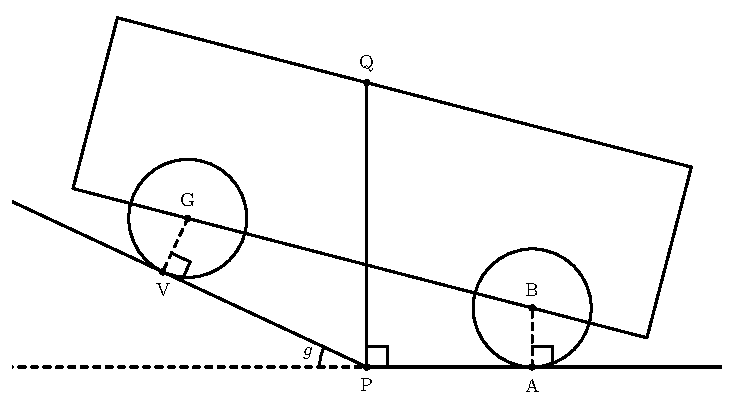
\includegraphics[width=.92\linewidth]{../figures/fhsm_2009_p64_2.pdf}
  \end{center}

After students work on the construction of a model, an interactive computer model can be given to students so that they can explore how changes in various trailer dimensions and positions can affect the dangerous height, $PQ$. One of these variables is the distance the trailer is under the bridge. Another, more subtle variable is the distance between the wheel axles. (By itself, the overhang of the trailer beyond either wheel axle does not affect the dangerous height and can be ignored.)

The next decision made by this class was to simplify the model even further during the first trip through the modeling cycle, taking the wheels off the truck. See the simplified model at the right. (The supporting topic book on geometry offers an analysis of the situation that uses the full model with the wheels on.)

  \begin{center}
    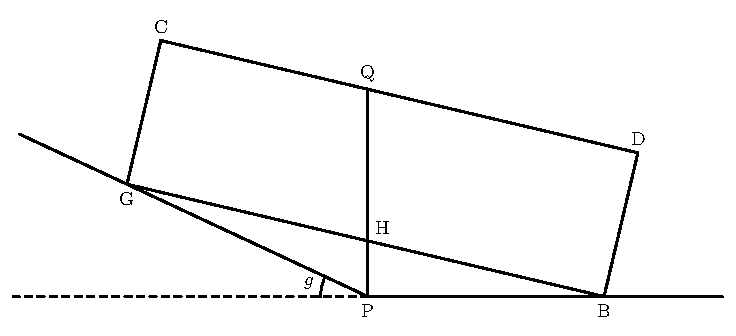
\includegraphics[width=.92\linewidth]{../figures/fhsm_2009_p65_1.pdf}
  \end{center}

\noindent
\textbf{Task 2}

Task 2 asks the students to examine what might be lost or misrepresented by this simplification. We do not provide a detailed classroom discussion of task 2. However, students should realize that taking the wheels off and lowering the shortened trailer box does not simply lower the dangerous height by an amount equal to the wheel radius. Rather, the left (raised) end of the truncated trailer box is lowered a bit more than the right end, and this positioning does have an additional measurable effect on the dangerous height. Nevertheless, an analysis of the simplified model will help us analyze the original situation with the more complex model, in which the trailer has wheels. Moreover, even in this simpler case with a small grade angle, the result may be surprising. 

Tasks 3 and 4 ask students to explore relationships in the simplified model both geometrically and symbolically.

\noindent
\textbf{Task 3}

Let $d$ represent the length of segment $PQ$, $w$ represent the measure of angle $PBH$ (the tilt of the trailer), $s$ represent the length of segment $PB$ (how far the trailer is under the bridge), and $g$ represent the grade in degrees. Explore the situation by using your interactive drawing of the simplified model. See if you can get a feel for---or make a conjecture about---when the dangerous height, $d$, would be highest by considering $w$ or $s$ or both.

  \begin{center}
    \includegraphics[width=.92\linewidth]{../figures/fhsm_2009_p66_1.pdf}
  \end{center}


\noindent
\textbf{In the Classroom (Second-Year Mathematics)}

One group used the interactive drawing to trace the graph of the dangerous height, $d$, as a function of $w$, as seen in the figure above, where they have set $g$ equal to $7$ degrees. They noted that they were not able to find a symbolic representation of this function but that it did suggest useful information. In their exploration, they used several small values of $g$, and each time the dangerous height looked greatest when

$$
  w=\frac{g}{2}.
$$

Another group used large angles for grades, for instance, 55 degrees, and that pattern did not hold up. But other students raised the objection that such large grades were unrealistic and not within bounds of the model. More insight was sought about what happens for small values of $g$.

After additional work, group 3 presented some theoretical evidence that adds some insight and support to the claim that the maximum value of the dangerous height occurs when

$$
  w=\frac{g}{2}
$$

for the (small) values of $g$ that our model allows.

Group 3 drew an analogy to example 15, ``Circling the Points,'' and envisioned $\angle GPB$ inscribed in a circle together with chord $GB$. The first thing to note is that the point $P$ changes position along the arc of the circle as the trailer box is drawn along the roadway. The perpendicular distance from $P$ to the chord $GB$ is greatest when the foot of this perpendicular, $K$, is the midpoint of segment $GB$.

  \begin{center}
    \includegraphics[width=.92\linewidth]{../figures/fhsm_2009_p66_2.pdf}
  \end{center}

\begin{scriptlist}
  \item [Student 3:] When $K$ is the midpoint of segment $GB$, angles $\angle PGB$ and $\angle PBG$ are congruent. I know that $m\angle PGB + m\angle PBG = m\angle SPG$, and the measure of angle $\angle SPG = g$. So now I have that

  $$
    m\angle PGB=m\angle PBG=\frac{g}{2}=w.
  $$

  Now I want to show that the part of the dangerous height represented by segment $PH$ is really close in length to segment $PK$---wherever $K$ is on $BG$. That is because the angle between segment $PK$ and segment $PH$ is small if $g$ is small. Here's why that is true. Triangles $PHK$ and $PHB$ are similar because they are right triangles that share $\angle PHK$. So $m\angle HPK = m\angle PBH = w$. But I know that $0 \leq w \leq g \leq 7^\circ$. Then $0.99 \leq \cos(w) \leq 1$. Since

  $$
    \cos(w)-\cos(\angle PHK)=\frac{\lvert PK\rvert}{\lvert PH\rvert},
  $$

  we've got that

  $$
    0.99\leq \frac{\lvert PK\rvert}{\lvert PH\rvert}\leq 1.
  $$

  This means the two lengths in the fraction are really, really close. \emph{The point is that part of the dangerous height represented by segment $PH$ should be maximized when the length of segment $PK$ is maximized, and that is when}

  $$
    m\angle PBG=\frac{g}{2}.
  $$

  \item [Teacher:] That gives some pretty solid support for the idea that there is at least a portion of the dangerous height that is at least close to being maximized when

  $$
    w=\frac{g}{2}.
  $$

  Let's continue by analyzing $d$ a little further.
\end{scriptlist}


\noindent
\textbf{Task 4}

Can you find a symbolic relationship between the tilt of the trailer, $w$, and the measure of the dangerous height $d$? You may use other measurements related to the model, such as $s$ (the distance the trailer is under the bridge, measured by segment $PB$), the length of the shortened trailer box (measured by segment $GB$), or some other measurement related to the situation. You may continue to find trigonometry useful.

\noindent
\textbf{In the Classroom (After Further Discussion)}

\begin{scriptlist}
  \item [Group 5:] We did find trigonometry helpful. We found a relationship between the length of segment $PH$ and $w$ first. We got that

  $$
    \tan(w)=\frac{\lvert PH\rvert}{\lvert PB\rvert}.
  $$

  So $\lvert PB\rvert\tan(w)=\lvert PH\rvert$. That is, $s\cdot \tan(w)=\lvert PH\rvert$.

  \begin{center}
    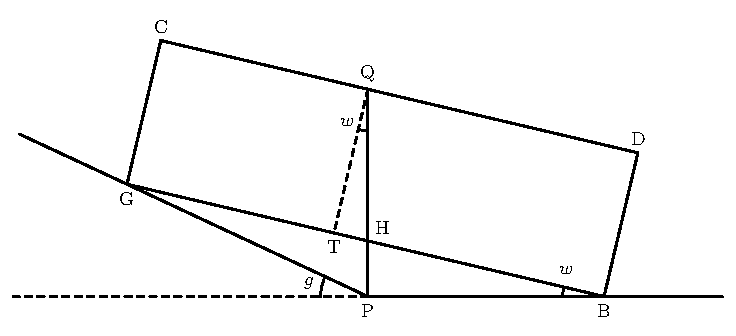
\includegraphics[width=.92\linewidth]{../figures/fhsm_2009_p68_1.pdf}
  \end{center}

  We wanted to find out something about the length of segment $HQ$ next. We didn’t get anywhere at first, but then one of our group members noticed that this segment sort of replaces the original height of the truck. So we decided to compare it to the original height of the truck. So then we drew segment $QT$ perpendicular to $GB$. The length of segment $QT$ would be the original height of the truck. After we drew the segment, we saw that $\angle PHB$ and $\angle THQ$ were congruent because they are vertical angles. That makes the right triangles $PHB$ and $THQ$ similar. So $\angle HQT = w$. We let $h$ stand for the original height of the truck. That is, $h =\lvert QT\rvert$. So

  $$
    \cos(w)=\frac{h}{\lvert HQ\rvert}.
  $$

  This means that

  $$
    \lvert HQ\rvert=\frac{h}{\cos(w)}.
  $$

  We put these together and got

  $$
    d=s\cdot \tan(w)+\frac{h}{\cos(w)}.
  $$

  \item [Teacher:] Good. That relationship works for any value of $w$ that occurs within the model. Now it is time to think about interpreting these results in the real world. What value of $g$ should we use in our formula?
  \item [Class:] Seven degrees.
  \item [Teacher:] We have gathered support for testing $w$ at

  $$
    \frac{g}{2},
  $$

  or $3.5$ degrees. For homework, research a good height to use for the trailer box and a good length for the trailer length between points $G$ and $B$. In addition, for

  $$
    w=\frac{g}{2}
  $$

  and $\lvert GB\rvert = m$, determine how one could figure out the value of $s$. We will need to do that to determine the value of $d$.
\end{scriptlist}

The next day students decide on $h = 10$ feet and $m = 40$ feet. In addition, $\triangle PGB$ is isosceles when

$$
  w=\frac{g}{2}.
$$

By constructing the altitude from $P$ to side $GB$, one can derive the relationship

$$
  \cos\left(\frac{g}{2}\right)=\frac{m/2}{s} \, \text{or} \, s=\frac{m/2}{\cos(g/2)}.
$$

With these values,

$$
  d=\frac{20}{\cos(3.5)}\tan(3.5)+\frac{10}{\cos(3.5)}\approx 11.24 \, \text{feet},
$$

or about $11$ feet $3$ inches. Just looking at the value $7$ degrees as a small number might suggest that road grade does not matter. But our analysis for this specific and realistic example shows that with an initial trailer height of $10$ feet, the dangerous height for the trailer is \emph{at least a foot higher}! As Dr. Pollak noted, road grade cannot be ignored.

\noindent
\textbf{Key Elements of Mathematics}

Reasoning with Geometry---Geometric connections and modeling; Construction and evaluation of geometric arguments

Reasoning with Algebraic Symbols---Meaningful use of symbols; Mindful
manipulation

Reasoning with Functions---Using multiple representations of functions

\noindent
\textbf{Reasoning Habits}

Analyzing the problem---identifying relevant variables and conditions; seeking patterns and relationships; looking for hidden structure; considering special cases or simpler analogs

Implementing a strategy---making purposeful use of procedures; making logical deductions; monitoring progress toward a solution

Seeking and using connections

Reflecting on a solution---considering the reasonableness of a solution; justifying or validating a solution; reconciling different approaches; generalizing a solution
}
{Qua gầm cầu}
{
\noindent
\textbf{Nhiệm vụ 1}

Nhà toán học Henry Pollak (2004) từng suy nghĩ về việc vì sao các xe đầu kéo kèm rơ-moóc thường bị mắc kẹt dưới một hầm chui nhất định, trong khi “độ tĩnh không tối đa” đã được ghi rõ trên một biển báo chỉ chiều cao của cây cầu. Cây cầu đang xét là nằm ngang và tọa lạc ngay tại chân của một con đường dốc xuống. Trong nhiệm vụ khởi đầu này, học sinh được yêu cầu xây dựng một mô hình trực quan hai chiều cho tình huống, đồng thời liệt kê những giả thiết mà các em đưa ra.

  \begin{center}
    \includegraphics[width=.92\linewidth]{../figures/fhsm_2009_p64_1.pdf}
  \end{center}

\noindent
\textbf{Trong lớp học (Toán năm thứ hai)}

Trong một mô hình trực quan, một bộ bánh xe của rơ-moóc được nâng lên trên phần đường dốc khi xe đi qua dưới mép cầu. Vị trí này khiến một phần của thùng xe bị nâng lên cao hơn so với khi xe ở trên mặt đường phẳng. Câu hỏi thực sự là: cao hơn bao nhiêu? Mô hình mà học sinh xây dựng nhiều khả năng sẽ có những đặc điểm tương tự mô hình trong hình vẽ bên dưới. Một mô hình như vậy tối thiểu phải chứa đoạn thẳng $PQ$---biểu thị “độ cao nguy hiểm” tại đó thùng xe có thể chạm vào cầu. Mô hình minh họa ở đây bao gồm những giả thiết đơn giản hóa, chẳng hạn biểu diễn bánh xe bằng các đường tròn và biểu diễn mặt đường bằng hai đoạn thẳng. Mỗi giả thiết đơn giản hóa đều cần được thảo luận trong lớp. Ngoài ra, sau một cuộc thảo luận hiệu quả, lớp có thể quyết định đo độ dốc của đường theo đơn vị độ thay vì theo phần trăm. Quyết định này được sử dụng trong phần phân tích tiếp theo. Một số nghiên cứu do học sinh thực hiện có thể gợi ý rằng đối với hầu hết các tuyến đường, độ dốc có thể được giới hạn hợp lý trong một khoảng nhỏ. Trong mô hình hiện tại, độ dốc của đường, $g$, được giới hạn đến $7$ độ---ít nhất là trong vòng lặp này của chu trình mô hình hóa. (Mặc dù độ dốc 7 độ có thể là khá lớn đối với một xe tải lớn, một số hình vẽ ở đây dùng góc dốc lớn hơn nhiều để làm nổi bật chi tiết.)

  \begin{center}
    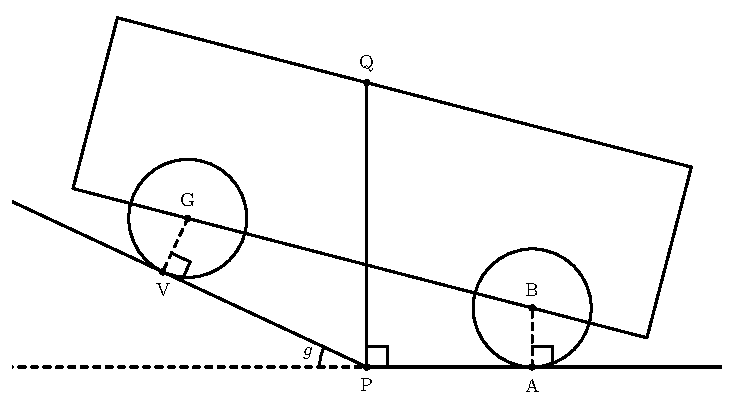
\includegraphics[width=.92\linewidth]{../figures/fhsm_2009_p64_2.pdf}
  \end{center}

Sau khi học sinh làm việc với việc xây dựng mô hình, có thể cung cấp cho các em một mô hình máy tính tương tác để các em khám phá việc thay đổi các kích thước và vị trí khác nhau của rơ-moóc có thể ảnh hưởng như thế nào đến độ cao nguy hiểm $PQ$. Một trong các biến số là khoảng cách mà rơ-moóc đã đi vào dưới gầm cầu. Một biến số khác, tinh tế hơn, là khoảng cách giữa hai trục bánh xe. (Tự thân phần thùng xe nhô ra vượt quá mỗi trục bánh xe không ảnh hưởng đến độ cao nguy hiểm và có thể bỏ qua.)

Quyết định tiếp theo của lớp là đơn giản hóa mô hình hơn nữa trong lượt đầu đi qua chu trình mô hình hóa, bằng cách tháo bánh xe khỏi xe tải. Xem mô hình đã đơn giản hóa ở hình bên phải. (Tài liệu chủ đề hỗ trợ về hình học cung cấp một phân tích tình huống dùng mô hình đầy đủ với bánh xe.)

  \begin{center}
    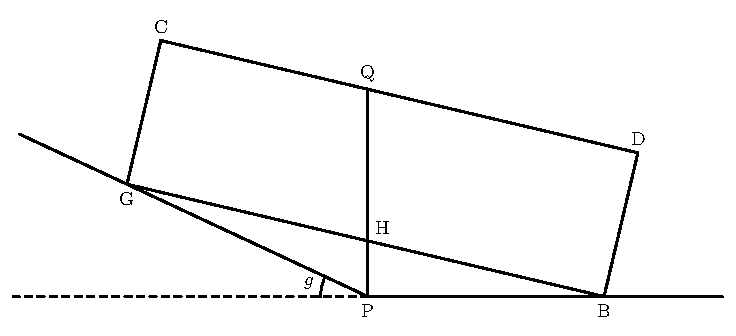
\includegraphics[width=.92\linewidth]{../figures/fhsm_2009_p65_1.pdf}
  \end{center}

\noindent
\textbf{Nhiệm vụ 2}

Nhiệm vụ 2 yêu cầu học sinh xem xét những điều có thể bị mất mát hoặc bị mô tả sai do sự đơn giản hóa này. Chúng tôi không trình bày chi tiết thảo luận trên lớp cho Nhiệm vụ 2. Tuy nhiên, học sinh cần nhận ra rằng việc tháo bánh xe và hạ thấp thùng xe đã rút ngắn không đơn giản chỉ làm giảm độ cao nguy hiểm đúng bằng bán kính bánh xe. Thay vào đó, đầu bên trái (đầu được nâng lên) của thùng xe bị hạ xuống nhiều hơn một chút so với đầu bên phải, và cách đặt này tạo ra một tác động bổ sung có thể đo được đối với độ cao nguy hiểm. Dẫu vậy, việc phân tích mô hình đơn giản hóa sẽ giúp chúng ta phân tích tình huống ban đầu với mô hình phức tạp hơn, trong đó rơ-moóc có bánh xe. Hơn nữa, ngay cả trong trường hợp đơn giản này với góc dốc nhỏ, kết quả vẫn có thể gây bất ngờ.

Nhiệm vụ 3 và 4 yêu cầu học sinh khám phá các mối quan hệ trong mô hình đơn giản hóa theo cả cách hình học lẫn cách ký hiệu.

\noindent
\textbf{Nhiệm vụ 3}

Gọi $d$ là độ dài đoạn $PQ$, gọi $w$ là số đo góc $PBH$ (độ nghiêng của thùng xe), gọi $s$ là độ dài đoạn $PB$ (mức độ thùng xe đã đi vào dưới gầm cầu), và gọi $g$ là độ dốc tính theo độ. Hãy khảo sát tình huống bằng cách sử dụng bản vẽ tương tác của mô hình đơn giản hóa. Hãy xem bạn có thể hình dung được---hoặc đưa ra một phỏng đoán về---khi nào độ cao nguy hiểm $d$ đạt lớn nhất bằng cách xét $w$ hoặc $s$ hoặc cả hai.

  \begin{center}
    \includegraphics[width=.92\linewidth]{../figures/fhsm_2009_p66_1.pdf}
  \end{center}


\noindent
\textbf{Trong lớp học (Toán năm thứ hai)}

One group used the interactive drawing to trace the graph of the dangerous height, $d$, as a function of $w$, as seen in the figure above, where they have set $g$ equal to $7$ degrees. They noted that they were not able to find a symbolic representation of this function but that it did suggest useful information. In their exploration, they used several small values of $g$, and each time the dangerous height looked greatest when

$$
  w=\frac{g}{2}.
$$

Một nhóm khác dùng những góc dốc lớn, chẳng hạn $55$ độ, và khi đó quy luật trên không còn đúng. Nhưng các học sinh khác phản đối rằng những độ dốc lớn như vậy là không thực tế và vượt ngoài giới hạn của mô hình. Lớp tiếp tục tìm hiểu điều gì xảy ra khi $g$ nhỏ.

Sau khi làm việc thêm, nhóm 3 trình bày một số bằng chứng mang tính lý thuyết, góp phần làm rõ và hỗ trợ cho khẳng định rằng giá trị lớn nhất của độ cao nguy hiểm xảy ra khi

$$
  w=\frac{g}{2}
$$

$$
  w=\frac{g}{2}
$$

đối với các giá trị (nhỏ) của $g$ mà mô hình của chúng ta cho phép.

Nhóm 3 liên hệ với Ví dụ 15, ``Đường tròn qua các điểm'', và hình dung rằng góc $\angle GPB$ là một góc nội tiếp của một đường tròn có dây cung là $GB$. Điều cần lưu ý đầu tiên là điểm $P$ thay đổi vị trí dọc theo cung tròn khi thùng xe được kéo dọc theo mặt đường. Khoảng cách vuông góc từ $P$ đến dây cung $GB$ đạt lớn nhất khi chân đường vuông góc này, $K$, là trung điểm của đoạn $GB$.

  \begin{center}
    \includegraphics[width=.92\linewidth]{../figures/fhsm_2009_p66_2.pdf}
  \end{center}

\begin{scriptlist}
  \item [Học sinh 3:] When $K$ is the midpoint of segment $GB$, angles $\angle PGB$ and $\angle PBG$ are congruent. I know that $m\angle PGB + m\angle PBG = m\angle SPG$, and the measure of angle $\angle SPG = g$. So now I have that

  $$
    m\angle PGB=m\angle PBG=\frac{g}{2}=w.
  $$

  Bây giờ em muốn chỉ ra rằng phần của độ cao nguy hiểm được biểu diễn bởi đoạn $PH$ có độ dài rất gần với đoạn $PK$---với mọi vị trí của $K$ trên $BG$. Đó là vì góc giữa đoạn $PK$ và đoạn $PH$ là nhỏ nếu $g$ nhỏ. Đây là lý do. Hai tam giác $PHK$ và $PHB$ đồng dạng vì chúng là các tam giác vuông và có chung một góc nhọn. Do đó $m\angle HPK = m\angle PBH = w$. Mà em biết $0^\circ \leq w \leq g \leq 7^\circ$. Khi đó $0.99 \leq \cos(w) \leq 1$. Vì

  $$
    \cos(w)-\cos(\angle PHK)=\frac{\lvert PK\rvert}{\lvert PH\rvert},
  $$

  nên ta có

  $$
    0.99\leq \frac{\lvert PK\rvert}{\lvert PH\rvert}\leq 1.
  $$

  Điều này có nghĩa là hai độ dài trong phân số là rất, rất gần nhau. \emph{Điểm mấu chốt là: phần của độ cao nguy hiểm được biểu diễn bởi đoạn $PH$ sẽ đạt lớn nhất khi độ dài đoạn $PK$ đạt lớn nhất, và điều đó xảy ra khi}

  $$
    m\angle PBG=\frac{g}{2}.
  $$

  \item [Giáo viên:] Lập luận đó cho thấy một sự hỗ trợ khá vững cho ý tưởng rằng có ít nhất một phần của độ cao nguy hiểm là gần như đạt cực đại khi

  $$
    w=\frac{g}{2}.
  $$

  Chúng ta hãy tiếp tục bằng cách phân tích $d$ sâu hơn một chút.
\end{scriptlist}


\noindent
\textbf{Nhiệm vụ 4}

Bạn có thể tìm một mối quan hệ ký hiệu giữa độ nghiêng của thùng xe, $w$, và độ lớn của độ cao nguy hiểm $d$ hay không? Bạn có thể dùng các đại lượng khác liên quan đến mô hình, chẳng hạn như $s$ (khoảng cách thùng xe đã đi vào dưới gầm cầu, đo bởi đoạn $PB$), độ dài thùng xe đã rút ngắn (đo bởi đoạn $GB$), hoặc một đại lượng khác liên quan đến tình huống. Bạn có thể tiếp tục thấy lượng giác hữu ích.

\noindent
\textbf{Trong lớp học (Sau thảo luận thêm)}

\begin{scriptlist}
  \item [Nhóm 5:] Chúng em thấy lượng giác hữu ích. Trước hết, chúng em tìm một quan hệ giữa độ dài đoạn $PH$ và $w$. Chúng em có

  $$
    \tan(w)=\frac{\lvert PH\rvert}{\lvert PB\rvert}.
  $$

  Vậy $\lvert PB\rvert\tan(w)=\lvert PH\rvert$. Tức là, $s\cdot \tan(w)=\lvert PH\rvert$.

  \begin{center}
    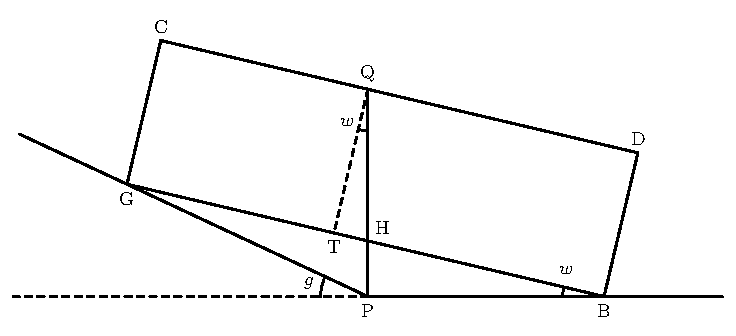
\includegraphics[width=.92\linewidth]{../figures/fhsm_2009_p68_1.pdf}
  \end{center}

  Tiếp theo, chúng em muốn tìm hiểu về độ dài đoạn $HQ$. Lúc đầu chúng em không đi đến đâu cả, nhưng rồi một bạn trong nhóm nhận ra rằng đoạn này giống như thay thế cho chiều cao ban đầu của xe tải. Vì vậy chúng em quyết định so sánh nó với chiều cao ban đầu của xe. Chúng em kẻ đoạn $QT$ vuông góc với $GB$. Độ dài đoạn $QT$ sẽ là chiều cao ban đầu của xe. Sau khi kẻ đoạn này, chúng em thấy $\angle PHB$ và $\angle THQ$ bằng nhau vì chúng là hai góc đối đỉnh. Do đó hai tam giác vuông $PHB$ và $THQ$ đồng dạng. Suy ra $\angle HQT = w$. Chúng em ký hiệu $h$ là chiều cao ban đầu của xe, tức là $h =\lvert QT\rvert$. Khi đó

  $$
    \cos(w)=\frac{h}{\lvert HQ\rvert}.
  $$

  Điều này cho thấy

  $$
    \lvert HQ\rvert=\frac{h}{\cos(w)}.
  $$

  Ghép các kết quả lại, chúng em được

  $$
    d=s\cdot \tan(w)+\frac{h}{\cos(w)}.
  $$

  \item [Giáo viên:] Tốt. Quan hệ đó đúng với mọi giá trị của $w$ xuất hiện trong mô hình. Bây giờ đã đến lúc nghĩ về việc diễn giải các kết quả này trong thế giới thực. Trong công thức của chúng ta, nên dùng giá trị nào của $g$?
  \item [Cả lớp:] Bảy độ.
  \item [Giáo viên:] Chúng ta đã thu thập được cơ sở để thử $w$ tại

  $$
    \frac{g}{2},
  $$

  tức $3.5$ độ. Về nhà, hãy tìm hiểu một chiều cao hợp lý để dùng cho thùng xe và một độ dài hợp lý cho phần chiều dài thùng xe giữa các điểm $G$ và $B$. Ngoài ra, với

  $$
    w=\frac{g}{2}
  $$

  và $\lvert GB\rvert = m$, hãy xác định cách tìm giá trị của $s$. Chúng ta sẽ cần điều đó để xác định $d$.
\end{scriptlist}

Ngày hôm sau, học sinh chọn $h = 10$ feet và $m = 40$ feet. Ngoài ra, tam giác $\triangle PGB$ cân khi

$$
  w=\frac{g}{2}.
$$

Bằng cách dựng đường cao từ $P$ xuống cạnh $GB$, ta suy ra hệ thức

$$
  \cos\left(\frac{g}{2}\right)=\frac{m/2}{s} \, \text{or} \, s=\frac{m/2}{\cos(g/2)}.
$$

Với các giá trị này,

$$
  d=\frac{20}{\cos(3.5)}\tan(3.5)+\frac{10}{\cos(3.5)}\approx 11.24 \, \text{feet},
$$

tức khoảng $11$ feet $3$ inch. Chỉ nhìn con số $7$ độ như một số nhỏ có thể khiến người ta nghĩ rằng độ dốc của đường không đáng kể. Nhưng phân tích của chúng ta trong ví dụ cụ thể và thực tế này cho thấy: với chiều cao ban đầu của thùng xe là $10$ feet, độ cao nguy hiểm của thùng xe \emph{*ít nhất cao hơn một foot*}! Như Dr. Pollak đã nhận xét, độ dốc của đường không thể bị bỏ qua.

\noindent
\textbf{Các yếu tố then chốt của toán học}

Luận với hình học---Các kết nối hình học và mô hình hóa; Xây dựng và thẩm định các lập luận hình học

Luận với ký hiệu đại số---Sử dụng ký hiệu có ý nghĩa; Biến đổi có ý thức

Luận với hàm số---Sử dụng nhiều biểu diễn của hàm số

\noindent
\textbf{Các thói quen luận}

Phân tích bài toán---xác định cẩn thận các biến và điều kiện thích đáng; tìm kiếm các mẫu hình và quan hệ; tìm kiếm cấu trúc ẩn; xét các trường hợp đặc biệt hoặc những
trường hợp tương tự đơn giản hơn

Triển khai chiến lược---vận dụng có chủ đích các thủ tục; thực hiện những suy diễn có tính luận lý; theo dõi tiến trình đi đến lời giải

Tìm kiếm và sử dụng các kết nối

Phản tư về lời giải---xem xét tính hợp lý của lời giải; biện minh hoặc kiểm chứng một lời giải; dung hòa các cách tiếp cận khác nhau; khái quát hóa lời giải
}
{}

\TriPara
{
\EN{The geometry strand extends beyond two- and three-dimensional figures in Euclidean space to include other special configurations and visualizations. Example 18 illustrates a modeling context in which the most obvious geometric model of the situation---drawing circles of radius $5$ units and looking for overlaps that represent radio interference---is not the most useful. Rather, a basic representation in the growing fi eld of “graph theory”---usually considered a domain within discrete mathematics---is better suited to capture the relevant information in the modeling problem.}
}
{
\VI{Mạch nội dung hình học không chỉ dừng lại ở các hình hai chiều và ba chiều trong không gian Euclid, mà còn mở rộng sang những cấu hình đặc biệt khác và các dạng trực quan hóa đa dạng. Ví dụ 18 minh họa một bối cảnh mô hình hóa trong đó mô hình hình học hiển nhiên nhất của tình huống---vẽ các đường tròn bán kính $5$ đơn vị và tìm các vùng chồng lấn biểu thị sự nhiễu sóng vô tuyến---lại không phải là mô hình hữu ích nhất. Thay vào đó, một cách biểu diễn cơ bản trong lĩnh vực đang phát triển của ``lý thuyết đồ thị''---thường được xem là một miền thuộc toán học rời rạc---lại phù hợp hơn để nắm bắt các thông tin then chốt trong bài toán mô hình hóa.}
}
{
\NOTE{}
}

\TriExample
{Assigning Frequencies}
{
\noindent
\textbf{Task}

The Federal Communications Commission (FCC) needs to assign radio frequencies to seven new radio stations located on the grid at the right. Such assignments are based on several considerations, including the possibility of creating interference by assigning the same frequency to stations that are too close together. In this simplified situation, we assume that broadcasts from two stations located within $200$ miles of each other will create interference if they broadcast on the same frequency, whereas stations more than $200$ miles apart can use the same frequency to broadcast without causing interference with each other.

\begin{center}
  \includegraphics[width=.92\linewidth]{../figures/fhsm_2009_p70_1.pdf}
\end{center}

How can a vertex-edge graph be used to assign frequencies so that the fewest number of frequencies are used and no stations interfere with each other? What would each vertex represent? What would an edge represent? What is the fewest number of frequencies needed? (Adapted from Hirsch et al. [2007])

\noindent
\textbf{In the Classroom}

Students work on the task in groups. Each group seems to agree that a vertex in the graph represents a radio station. So the graph would have seven vertices. Some groups decide to make a graph model in which two vertices representing stations within 200 miles of each other will be joined by an edge.

\begin{center}
  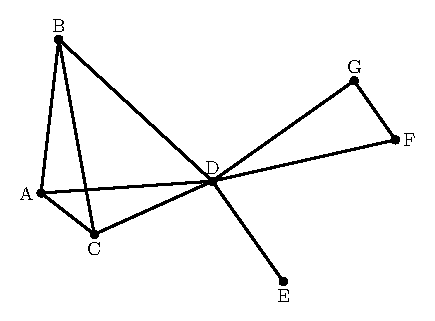
\includegraphics[width=.92\linewidth]{../figures/fhsm_2009_p71_1.pdf}
\end{center}

Other groups suggest that two vertices will be joined with an edge if they are *more* than 200 miles apart. After some discussion, the choice is made to use the first suggestion, that of joining vertices with an edge if the distance between them is no more than 200 miles. The next task is to construct the model. Doing so requires computation of the distance between each pair of stations. Groups make these computations by using the distance formula or Pythagorean theorem and a calculator. Organization is valuable here because many computations are involved. Some groups might start by computing the distance from $A$ to the remaining six stations, then the distance from $B$ to the remaining five, and so on. A quick determination of how many computations are needed can help determine whether any list is missing an item. Experience with example 10, ``Patterns, Plane and Symbol,'' would be useful in this context.

Groups produce models similar to the one above and then work at assigning frequencies to vertices so that no two vertices joined by a single edge have the same frequency. They look for a method that will use the fewest frequencies for this particular graph. One group explained their solution this way:

``We found that the fewest number of frequencies that could be used was four. We reasoned this way: First, look at the collection of vertices $A$ through $D$. Each of these vertices is joined by an edge to each of the other three in the collection. So no two vertices in the collection can have the same frequency. That means you can have no fewer than four frequencies.

Next, suppose you assign frequency 1 to vertex $A$, frequency 2 to vertex $B$, frequency 3 to vertex $C$, and frequency 4 to vertex $D$. You can finish the assignment by assigning frequency 1 to vertex $G$ (because $G$ doesn't interfere with $A$), frequency 2 to vertex $F$, and frequency 3 to vertex $E$. That proves you don't need any more than four frequencies. That does it!''

\noindent
\textbf{Key Elements of Mathematics}

Reasoning with Geometry---Geometric connections and modeling; Construction of geometric arguments

\noindent
\textbf{Reasoning Habits}

Analyzing a problem---seeking patterns and relationships; applying previously learned concepts

Implementing a strategy---organizing a solution; making logical deductions

Reflecting on a solution---justifying or validating a solution
}
{Xếp tần số}
{
\noindent
\textbf{Nhiệm vụ}

Ủy ban Truyền thông Liên bang Hoa Kỳ (Federal Communications Commission---FCC) cần phân bổ các tần số vô tuyến cho bảy đài phát thanh mới, được đặt tại các vị trí trên lưới tọa độ như trong hình bên dưới. Việc phân bổ này dựa trên nhiều yếu tố, trong đó có khả năng xảy ra nhiễu sóng khi gán cùng một tần số cho các đài ở quá gần nhau. Trong tình huống đã được đơn giản hóa này, ta giả sử rằng các đài phát thanh cách nhau không quá $200$ dặm sẽ gây nhiễu nếu cùng phát trên một tần số, trong khi các đài cách nhau hơn $200$ dặm có thể sử dụng cùng một tần số mà không gây nhiễu cho nhau.

\begin{center}
  \includegraphics[width=.92\linewidth]{../figures/fhsm_2009_p70_1.pdf}
\end{center}

Làm thế nào có thể sử dụng một đồ thị đỉnh-cạnh để phân bổ tần số sao cho số lượng tần số sử dụng là ít nhất và không có đài nào gây nhiễu cho đài khác? Mỗi đỉnh sẽ biểu diễn điều gì? Mỗi cạnh sẽ biểu diễn điều gì? Số lượng tần số ít nhất cần dùng là bao nhiêu? (Phỏng theo Hirsch và cộng sự [2007])

\noindent
\textbf{Trong lớp học}

Học sinh làm việc theo nhóm để giải quyết nhiệm vụ. Mỗi nhóm đều đồng ý rằng một đỉnh trong đồ thị sẽ biểu diễn một đài phát thanh. Do đó, đồ thị sẽ có bảy đỉnh. Một số nhóm quyết định xây dựng mô hình đồ thị trong đó hai đỉnh biểu diễn các đài cách nhau không quá $200$ dặm sẽ được nối với nhau bằng một cạnh.

\begin{center}
  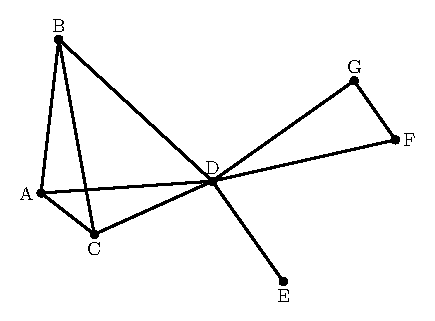
\includegraphics[width=.92\linewidth]{../figures/fhsm_2009_p71_1.pdf}
\end{center}

Một số nhóm khác đề xuất rằng hai đỉnh sẽ được nối với nhau bằng một cạnh nếu chúng cách nhau \emph{hơn} $200$ dặm. Sau một hồi thảo luận, lớp quyết định chọn phương án thứ nhất: nối hai đỉnh bằng một cạnh nếu khoảng cách giữa hai đài tương ứng không vượt quá $200$ dặm.

Nhiệm vụ tiếp theo là xây dựng mô hình. Việc này đòi hỏi phải tính khoảng cách giữa từng cặp đài. Các nhóm thực hiện các phép tính này bằng cách sử dụng công thức khoảng cách hoặc định lý Pythagoras cùng với máy tính cầm tay. Việc tổ chức có vai trò quan trọng ở đây, vì số lượng phép tính là khá nhiều. Một số nhóm có thể bắt đầu bằng cách tính khoảng cách từ đài $A$ đến sáu đài còn lại, sau đó từ $B$ đến năm đài còn lại, và cứ tiếp tục như vậy. Việc nhanh chóng xác định cần bao nhiêu phép tính sẽ giúp kiểm tra xem danh sách có bị thiếu trường hợp nào hay không. Kinh nghiệm từ Ví dụ 10, ``Thêm đường thêm miền'', sẽ hữu ích trong bối cảnh này.

Các nhóm tạo ra những mô hình tương tự như hình trên và sau đó tiến hành gán tần số cho các đỉnh sao cho không có hai đỉnh nào được nối trực tiếp bởi một cạnh lại có cùng tần số. Các em tìm kiếm một phương pháp cho phép sử dụng ít tần số nhất cho đồ thị cụ thể này. Một nhóm đã trình bày lời giải của mình như sau:

``Chúng em nhận thấy rằng số lượng tần số ít nhất có thể dùng là bốn. Lập luận của chúng em như sau: Trước hết, xét tập các đỉnh từ $A$ đến $D$. Mỗi đỉnh trong tập này đều được nối bằng một cạnh với ba đỉnh còn lại trong tập. Vì vậy, không có hai đỉnh nào trong tập này có thể có cùng một tần số. Điều đó có nghĩa là không thể dùng ít hơn bốn tần số.

Tiếp theo, giả sử ta gán tần số 1 cho đỉnh $A$, tần số 2 cho đỉnh $B$, tần số 3 cho đỉnh $C$, và tần số 4 cho đỉnh $D$. Ta có thể hoàn tất việc gán bằng cách gán tần số 1 cho đỉnh $G$ (vì $G$ không gây nhiễu với $A$), tần số 2 cho đỉnh $F$, và tần số 3 cho đỉnh $E$. Điều đó chứng tỏ ta không cần dùng nhiều hơn bốn tần số. Như vậy là xong!''

\noindent
\textbf{Các yếu tố then chốt của toán học}

Luận với hình học---Các kết nối hình học và mô hình hóa; Xây dựng và thẩm định các lập luận hình học

\noindent
\textbf{Các thói quen luận}

Phân tích bài toán---tìm kiếm các mẫu hình và quan hệ; vận dụng các khái niệm đã học

Triển khai chiến lược---tổ chức lời giải; thực hiện những suy diễn có tính luận lý

Phản tư về lời giải---biện minh hoặc kiểm chứng một lời giải
}
{}

\TriPara
{
\EN{Note that the vertex-edge representation of the frequency-assignment problem seems to have facilitated the structuring of an argument that four frequencies suffice---and even a way (algorithm) to assign four frequencies---for this example. Finding efficient algorithms for analogues of the general fewest-frequency problem for larger graphs remains an active area of current mathematical research. Such algorithms would find uses in many contexts.}
}
{
\VI{Lưu ý rằng cách biểu diễn bài toán phân bổ tần số bằng đồ thị đỉnh-cạnh dường như đã giúp cấu trúc hóa một lập luận mà bốn tần số là đủ---đồng thời còn gợi ra một cách (thuật toán) để gán bốn tần số trong ví dụ này. Việc tìm kiếm các thuật toán hiệu quả cho những bài toán tương tự của bài toán ``ít tần số nhất'' trong trường hợp các đồ thị lớn hơn hiện vẫn là một lĩnh vực nghiên cứu toán học đang phát triển mạnh. Những thuật toán như vậy có tiềm năng được ứng dụng trong nhiều bối cảnh khác nhau.}
}
{
\NOTE{}
}

\TriPara
{
\EN{
Geometry offers an inviting context in which students can develop their reasoning and sense making abilities. In addition, geometry provides tools and representations that are useful in a wide range of situations.}
}
{
\VI{Hình học mang đến một bối cảnh giàu sức gợi, trong đó học sinh có thể phát triển năng lực luận và hiểu. Bên cạnh đó, hình học còn cung cấp những công cụ và cách biểu diễn hữu ích, có thể được vận dụng trong nhiều tình huống đa dạng.}
}
{
\NOTE{}
}

% =========
% CHƯƠNG 8
% =========

\ParallelChapter
  {Reasoning with Statistics and Probability}
  {Luận với thống kê và xác suất}
  {}

\TriPara
{
\EN{In our increasingly data-intensive world, statistics is one of the most important areas of the mathematical sciences for helping students make sense of the information all around them, as well as for preparing them for further study in a variety of disciplines (e.g., the health sciences, the social sciences, and environmental science) for which statistics is a fundamental tool for advancing knowledge. Competence in the Standards found in \emph{Principles and Standards} (NCTM 2000a) depends on a thorough and deep understanding of the foundations of statistics and probability, and of the connections between statistics and probability. Taken together, \emph{Principles and Standards} and the American Statistical Association's report \emph{Guidelines for Assessment and Instruction in Statistics Education} (GAISE) (Franklin et al. 2007) describe statistical problem solving as an investigative process that involves the following four components:

\begin{itemize}
  \item Formulating a question (or questions) that can be addressed with data
  \item Designing and employing a plan for collecting data
  \item Analyzing and summarizing the data
  \item Interpreting the results from the analysis, and answering the question on the basis of the data
\end{itemize}}
}
{
\VI{Trong một thế giới ngày càng đậm đặc dữ liệu như hiện nay, thống kê là một trong những lĩnh vực quan trọng nhất của khoa học toán học trong việc giúp học sinh hiểu lượng thông tin bao quanh mình, đồng thời chuẩn bị cho các em tiếp tục học tập trong nhiều ngành khác nhau, chẳng hạn khoa học sức khỏe, khoa học xã hội, và khoa học môi trường, những lĩnh vực mà thống kê là một công cụ nền tảng để thúc đẩy tri thức tiến lên. Năng lực đáp ứng các Chuẩn được nêu trong \emph{Principles and Standards} (NCTM 2000a) phụ thuộc vào một sự hiểu biết vừa vững vừa sâu về những nền tảng của thống kê và xác suất, cũng như về các mối liên hệ giữa thống kê và xác suất. Khi được đọc cùng nhau, \emph{Principles and Standards} và báo cáo của Hiệp hội Thống kê Hoa Kỳ mang tên \emph{Guidelines for Assessment and Instruction in Statistics Education} (GAISE) (Franklin et al. 2007) mô tả việc giải quyết vấn đề thống kê như một quá trình khảo sát gồm bốn thành phần sau:

\begin{itemize}
  \item Hình thành một câu hỏi, hoặc một nhóm câu hỏi, có thể được trả lời bằng dữ liệu
  \item Thiết kế và triển khai một kế hoạch thu thập dữ liệu
  \item Phân tích và tóm lược dữ liệu
  \item Diễn giải các kết quả phân tích, và trả lời câu hỏi trên cơ sở dữ liệu
\end{itemize}}
}
{
\NOTE{}
}

\TriPara
{
\EN{The common thread throughout the statistical problem-solving process is the focus on making sense of, and reasoning about, variation in data. The goal is not only to solve problems in the presence of variation but also to provide a measure of how much the variation might affect the solution. This process provides a framework for teaching and learning statistics in school, and meaningful tasks that employ this process should permeate the statistical education of our students.}
}
{
\VI{Sợi chỉ xuyên suốt toàn bộ quá trình giải quyết vấn đề thống kê là sự tập trung vào việc hiểu và luận về độ biến thiên trong dữ liệu. Mục tiêu không chỉ là giải quyết các bài toán trong sự hiện diện của biến thiên, mà còn là đưa ra một thước đo cho biết biến thiên ấy có thể ảnh hưởng đến lời giải ở mức nào. Quá trình này tạo nên một khung sườn cho việc dạy và học thống kê trong nhà trường, và những nhiệm vụ có ý nghĩa, vận dụng tiến trình ấy, cần thấm vào toàn bộ quá trình giáo dục thống kê của học sinh.}
}
{
\NOTE{``Sự biến thiên'' là trọng tâm cốt lõi của lập luận thống kê. Thống kê không tìm cách loại bỏ biến thiên, mà học cách hiểu, mô tả và lập luận với biến thiên như một đặc trưng tất yếu của dữ liệu trong thế giới thực.

Việc nhấn mạnh rằng mục tiêu không chỉ là tìm lời giải, mà còn là đánh giá mức độ ảnh hưởng của biến thiên đối với lời giải, cho thấy sự khác biệt căn bản giữa tư duy thống kê và các hình thức luận toán học mang tính xác định. Trong thống kê, một kết quả chỉ có ý nghĩa khi đi kèm với mức độ tin cậy hoặc phạm vi ảnh hưởng của sự không chắc chắn.

Tiến trình giải quyết vấn đề thống kê không chỉ là một mô hình kỹ thuật, mà là một khung sư phạm định hướng cho toàn bộ việc dạy và học thống kê. Theo đó, các nhiệm vụ học tập có ý nghĩa cần được thiết kế sao cho học sinh thường xuyên đối diện với dữ liệu có biến thiên và buộc phải luận về biến thiên đó, thay vì chỉ thực hiện các thao tác tính toán rời rạc.}
}

\TriPara
{
\EN{Key elements of reasoning and sense making with statistics and probability include the following:

\begin{itemize}
  \item \emph{Data analysis.} Gaining insight about a solution to a statistics question by collecting data and describing features of the data through the use of graphical and tabular representations and numerical summaries. (The interpretation of results in data analysis encompasses both empirical and informal levels of reasoning, as described in the progression of reasoning in chapter 2.)
  \item \emph{Modeling variability.} Developing probability models to describe the long-run behavior of observations of a random variable.
  \item \emph{Connecting statistics and probability.} Recognizing probability as an essential tool of statistics; understanding the role of probability in statistical reasoning.
  \item \emph{Interpreting designed statistical studies.} Drawing appropriate conclusions from data in ways that acknowledge random variation. (Interpreting results from designed statistical studies involves statistical inference and other more formal levels of statistical reasoning.)
\end{itemize}

We address these key elements in more detail in the following sections.}
}
{
\VI{Các yếu tố then chốt của luận và hiểu với thống kê và xác suất gồm có:

\begin{itemize}
  \item \emph{Phân tích dữ liệu.} Hình thành hiểu biết về lời giải cho một câu hỏi thống kê bằng cách thu thập dữ liệu và mô tả các đặc trưng của dữ liệu thông qua việc sử dụng các biểu diễn bằng đồ thị, bảng biểu và các đại lượng tóm tắt bằng số. (Việc diễn giải các kết quả trong phân tích dữ liệu bao hàm cả những mức độ luận thực nghiệm và không hình thức, như đã được mô tả trong tiến trình của luận ở Chương 2.)
  \item \emph{Mô hình hóa biến thiên.} Xây dựng các mô hình xác suất để mô tả hành vi dài hạn của các quan sát của một biến ngẫu nhiên.
  \item \emph{Kết nối thống kê và xác suất.} Nhận ra xác suất là một công cụ cốt yếu của thống kê; hiểu vai trò của xác suất trong luận thống kê.
  \item \emph{Diễn giải các nghiên cứu thống kê có thiết kế.} Rút ra những kết luận thích hợp từ dữ liệu theo những cách có tính đến biến thiên ngẫu nhiên. (Việc diễn giải các kết quả từ những nghiên cứu thống kê có thiết kế bao hàm suy luận thống kê và những mức độ luận thống kê hình thức hơn.)
\end{itemize}

Chúng tôi sẽ trình bày chi tiết hơn các yếu tố then chốt này trong các phần tiếp theo.}
}
{
\NOTE{}
}

\ParallelSection
  {Data Analysis}
  {Phân tích dữ liệu}
  {}

\TriPara
{
\EN{Data analysis is more than simply the analysis of data. Data analysis includes all four components described in the process of statistical problem solving. Data are observations or measurements collected on one or more variables to address a statistical question. In statistics, a variable is any characteristic for which individual observations can be expected to take different values. Consequently, data vary and, once collected, need to be summarized in ways that foster meaningful insights for addressing the question under study. The analysis of data includes exploring various representations of the \emph{data distribution} to summarize and describe patterns and relationships in the variation and to identify deviations from a pattern. Technology provides the opportunity to examine various representations of the data distribution and to identify important features of the distribution. In data analysis, the interpretation of results includes both empirical and informal levels of reasoning. Because both numerical data and numerical summaries of data are used in data analysis, statistics has connections with the Numbers and Measurements strand described in chapter 4, particularly the key elements of \emph{reasonableness of answers and measurements and approximations and error}.}
}
{
\VI{Phân tích dữ liệu không chỉ đơn thuần là việc xử lý dữ liệu. Phân tích dữ liệu bao gồm đầy đủ cả bốn thành phần đã được mô tả trong tiến trình giải quyết vấn đề thống kê. Dữ liệu là các quan sát hoặc phép đo được thu thập trên một hay nhiều biến nhằm trả lời một câu hỏi thống kê. Trong thống kê, một biến là bất kỳ đặc trưng nào mà các quan sát riêng lẻ có thể được kỳ vọng là nhận những giá trị khác nhau. Do đó, dữ liệu luôn có sự biến thiên và, sau khi được thu thập, cần được tóm tắt theo những cách giúp tạo lập ý nghĩa để giải quyết câu hỏi đang được nghiên cứu. Phân tích dữ liệu bao gồm việc khảo sát các biểu diễn khác nhau của \emph{phân bố dữ liệu} nhằm tóm tắt và mô tả các khuôn mẫu và mối quan hệ trong sự biến thiên, cũng như để nhận diện những sai lệch so với một khuôn mẫu. Công nghệ tạo điều kiện cho việc xem xét nhiều biểu diễn khác nhau của phân bố dữ liệu và xác định những đặc trưng quan trọng của phân bố đó. Trong phân tích dữ liệu, việc diễn giải kết quả bao hàm cả các mức độ luận thực nghiệm và phi hình thức. Do cả dữ liệu dạng số và các đại lượng tóm tắt bằng số của dữ liệu đều được sử dụng trong phân tích dữ liệu, nên thống kê có mối liên hệ với mạch \emph{Số và Đo lường} được trình bày ở Chương 4, đặc biệt là các yếu tố cốt lõi về \emph{tính hợp lý của kết quả, đo lường, xấp xỉ và sai số}.}
}
{
\NOTE{}
}

\TriPara
{
\EN{Example 19 shows how statistical procedures for analyzing data that are developed in earlier grades continue to be useful tools for making sense of, and reasoning about, data in high school. Example 19 illustrates organizing and interpreting a solution and recognizing the scope of inference for a statistical solution. A detailed description of this activity is given in Kader and Mamer
(2008).}
}
{
\VI{Ví dụ 19 cho thấy các quy trình thống kê dùng trong phân tích dữ liệu, vốn đã được hình thành từ các lớp học trước, vẫn tiếp tục là những công cụ hữu ích giúp học sinh kiến tạo hiểu và luận về dữ liệu ở bậc trung học phổ thông. Ví dụ này minh họa việc tổ chức và diễn giải một lời giải, đồng thời nhận ra phạm vi suy luận mà một lời giải thống kê cho phép. Mô tả chi tiết về hoạt động này được trình bày trong công trình của Kader và Mamer (2008).}
}
{
\NOTE{}
}

\TriExample
{Meaningful Words, Part A}
{
\begin{center}
  Adapted from WGBH Educational Foundation (2001)
\end{center}

\noindent
\textbf{Task}

Scientists are interested in human recall and memory. Is it easier to memorize words that have ``meaning?'' To study this problem, two lists of 20 three-letter ``words'' were used. One list contained meaningful words (e.g., CAT, DOG), whereas the other list contained nonsense words (e.g., ATC, ODG). A ninth-grade class of thirty students was randomly divided into two groups of fifteen students. One group was asked to memorize the list of meaningful words; the other group was asked to memorize the list of nonsense words. The number of words correctly recalled by each student was tabulated, and the resulting data are as follows:

Number of meaningful words recalled: $12$, $15$, $12$, $12$, $10$, $3$, $7$, $11$, $9$, $14$, $9$, $10$, $9$, $5$, $13$ 

Number of nonsense words recalled: $4$, $6$, $6$, $5$, $7$, $5$, $4$, $7$, $9$, $10$, $4$, $8$, $7$, $3$, $2$

\begin{enumerate}
  \item Provide a display for summarizing and comparing these data sets.
  \item On the basis of your display, what observations can be made regarding how the students assigned the meaningful words performed compared with how the students assigned the nonsense words performed? Write a paragraph summarizing what the data and your analysis reveal about the question ``Is it easier to memorize words that have meaning?''
\end{enumerate}

\noindent
\textbf{In the Classroom (Ninth-Grade Mathematics Class)}

Several groups of students created comparative dotplots for the data, as shown below.

\begin{center}
  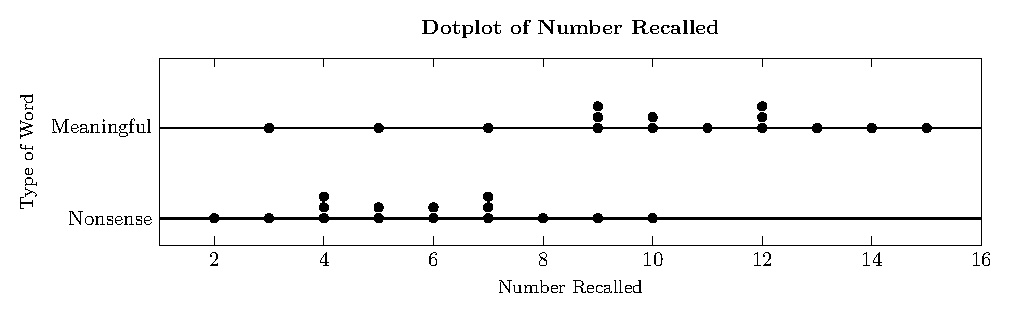
\includegraphics[width=.92\linewidth]{../figures/fhsm_2009_p75_1.pdf}
\end{center}

\begin{scriptlist}
  \item [Teacher:] Looking at the dotplots, for which type of words did students generally have better recall? How do you know? Give some specific reasons for your answer.
  \item [Student A:] A lot of students with the meaningful words did better. The highest number recalled is ten for the students with the nonsense words. Seven of the students with meaningful words recalled more than ten words, and ten is the best for all the students with the nonsense words.
  \item [Student B:] Yes, but some of the students with the meaningful words did not do very well, either. One recalled only three words; another, only fi ve words; and another, only seven words. These seem low for the meaningful words.
  \item [Student C:] Yes, and there are some gaps in the low end of the meaningful-words data distribution but not so much in the nonsense-words distribution. A lot of the students with the nonsense words recalled between three and seven words, and only a few of the students with the meaningful words recalled between three and seven words.
  \item [Teacher:] Can you be more specific?
  \item [Student C:] Well, three out of the fifteen students with the meaningful words recalled between three and seven words. That's only 20 percent. For the students using the nonsense words, eleven out of fifteen, more than 73 percent, recalled that many. If you add the student who only recalled two nonsense words, twelve out of these fifteen students, that's 80 percent, recalled between two and seven words, whereas only 20 percent of the students with the meaningful words were this low. In fact, all fifteen students using the nonsense words recalled between two and ten words, but only eight students with the meaningful words were this low. 
  \item [Teacher:] That's the same as what student A said, seven of the fifteen students using the meaningful-words list recalled more words than any of the students using the nonsense-words list. That means close to half the students memorizing the meaningful words did better than all students with the nonsense words.
  \item [Teacher:] Let's try to identify a typical value for the number of words recalled for each list. What quantity would you propose?
  \item [Student D:] We could find the average number recalled for each list.
  \item [Teacher:] Why do you propose the average, which is also called the mean?
  \item [Student D:] Well, it seems like we always find the mean whenever we want to know a typical value.
  \item [Student E:] Yes, sometimes the mean is good. But sometimes we use the median for a typical value.
  \item [Teacher:] In this case, does it matter which one you use?
  \item [Student E:] Well, in the dotplot for the meaningful words, three of the values look kind of small. I think these three values might make the mean smaller than what's typical. So I would use the median instead of the mean.
  \item [Teacher:] Very good. When we see a graph of data like the dotplot for the meaningful words, we say the shape of the data distribution is skewed to the left. Like student E said, when a data distribution is skewed left, the mean is often smaller than what one might think of as typical for the data. For this reason, the median might provide a better indication of how many words were typically recalled by students with the meaningful list. So, what would you propose for a typical value for the number of words recalled by students with the nonsense-words list?
  \item [Student E:] The data distribution for the nonsense list looks pretty even. I think this indicates it has a symmetrical shape. So you could probably use either the mean r the median for these data. Since we are using the median for the meaningful words, and it would not make sense to compare the mean of one group to the median of another group, I would use the median for the nonsense words as well.
  \item [Teacher:] What do the rest of you think? What happens when we use the medians?
  \item [Student D:] My calculator gives the median for the meaningful words as $10$, and for the nonsense words the median is $6$. 
  \item [Teacher:] What if we did not have the data values, but only knew the medians? What do the medians tell us about the data?
  \item [Student D:] The median divides the data in half.
  \item [Teacher:] Yes, so if the median is ten words for the data on meaningful words, what can we say about the rest of the data?
  \item [Student F:] About half the students assigned to the meaningful-words list remembered fewer than ten words, and about half remembered more than ten words.
  \item [Teacher:] Comparing the two medians, what would you conclude?
  \item [Student F:] The median for the meaningful words is ten words, but the median for the nonsense words is six words. Ten is higher than six, so students with meaningful words typically did better than the students with nonsense words.
  \item [Teacher:] This is an interesting observation. Another way of looking at this is to say that the difference between the medians is four words. So students with the meaningful words typically recalled four more words than students with the nonsense list.
  \item [Teacher:] If only the medians are reported for these data, what information about the number of words recalled is missing?
  \item [Student G:] If all you know is the median, you don't know the actual number recalled for each student. Take the data for the meaningful words. If all I know is that the median number recalled is ten words, I don't really know about the different values that actually occurred. For example, looking at the student who remembered only three words, three words is a lot different from ten words.
  \item [Teacher:] So, student G, what is the idea you talking about called?
  \item [Student G:] The number of words recalled is not the same for each student. I think this is the idea of variability in the data, which we have talked about before.
  \item [Teacher:] Yes, you are correct. In statistics, we are interested in representing the data with a typical value, such as the median, but we are also interested in summarizing the amount of variability in the data, as well. Does anyone have any suggestions for how we might do this?
  \item [Student H:] We could find the ranges. I think this tells us something about how much variability there is. The range is 12 for the meaningful list. The range for the nonsense list is $8$.
  \item [Teacher:] So, what do the ranges suggest about the variation in the data?
  \item [Student H:] The biggest difference between any two values from the meaningful list is twelve words, but the biggest difference between any two values from the nonsense list is eight words. This says that there is more variability in the number of words recalled on the meaningful words list than on the nonsense words list.
  \item [Student I:] Yes, but the smallest value from the meaningful words seems really small. For this reason, I don't think I would use the ranges. Instead, I think we should find the quartiles and use the interquartile ranges (IQR) instead. Then I am comparing the amount of variation for the middle portions of each group.
  \item [Teacher:] How do you find the IQR?
  \item [Student I:] First you have to find the first and third quartiles for each group of data. Then you find the range between the quartiles. You subtract the first quartile from the third quartile.
  \item [Teacher:] OK. Everyone find the quartiles and the interquartile ranges.
  \item [Student J:] For the meaningful words, my calculator gives the first quartile as nine words and the third quartile as twelve words. So the IQR is three words. For the nonsense words, the first quartile is four words and the third quartile is seven words. So the IQR is three words. The IQRs are the same, so there are similar amounts of variation in the middle 50 percent of the data for both the meaningful words and the nonsense words.
  \item [Student K:] My calculator gives five quantities for each group-the minimum, the first quartile, the median, the third quartile, and the maximum. I think we can get a graph called a box-and-whiskers plot by using these five numbers.
  \item [Teacher:] Yes, you can. When you include an outlier analysis, it is called a modified boxplot.
\end{scriptlist}

The class used results from a calculator to produce the following comparative modified boxplots:


\begin{center}
  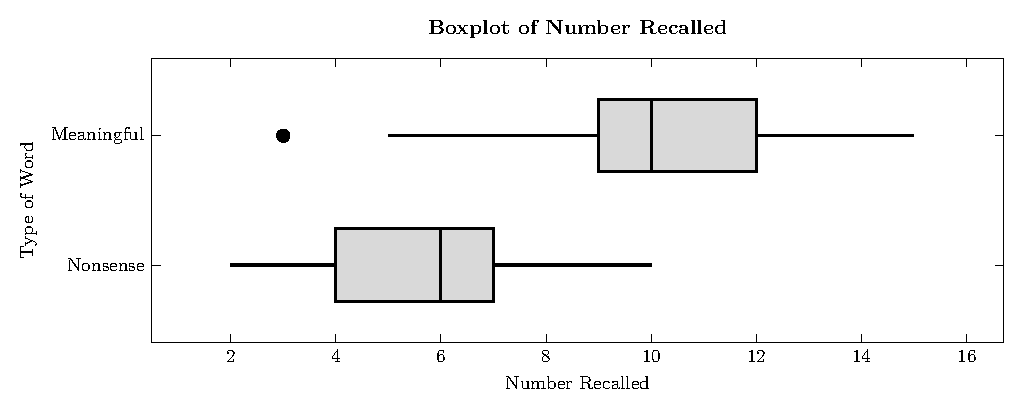
\includegraphics[width=.92\linewidth]{../figures/fhsm_2009_p79_1.pdf}
\end{center}

\begin{scriptlist}
  \item [Teacher:] Can you use the results from the boxplots to summarize our discussions about this question?
  \item [Student M:] Students with the list of meaningful words generally recalled more words. The maximum number of words recalled for the students with the nonsense list is ten. Ten is the median number recalled for the meaningful list, so about half the students with the meaningful words recalled more words than any of the student with the nonsense words. With the meaningful words, one student recalled only three words, and this score is an outlier and somewhat lower than expected when compared to the other data. The median number recalled with the meaningful words is ten, which is four more words than the median number recalled from the nonsense words. Excluding the outlier from the meaningful-words data, both groups appear to have similar amounts of variation. The IQR for each group is 3, indicating that for both meaningful and nonsense words the number of words recalled within the middle 50 percent differ by no more than three words.
  \item [Teacher:] What do these results suggest about memory and meaning?
  \item [Student N:] Since students with the meaningful words seemed to do better, these data suggest it is easier to memorize words that have meaning.
  \item [Teacher:] Do you think it would be appropriate to say that all ninth graders would get exactly the same results?
  \item [Student O:] Sure, it's easier to memorize words that have meaning.
  \item [Student P:] Well, we would not get exactly the same scores! But we might still see that words with meaning will be easier to memorize.
  \item [Teacher:] We have to be careful about our scope of inference, or trying to generalize these results to other ninth graders based on these data. The scope of inference depends on whether or not the studied class is representative of all ninth-grade classes. As we don't know how the class was selected, we should not try to generalize the results to all ninth-grade classes or to all ninth graders. If a group of ninth-grade students is selected at random, then we might try to generalize these results to all ninth graders.
  \item [Student Q:] But I thought they used randomness in the study.
  \item [Teacher:] Yes, they did. However, randomness was used in assigning the students to the different groups. The reason for using random assignment is to produce two comparable groups. For example, you would not want all students who are good at memorizing in one group. By randomly assigning the students to the two groups, we hope to balance the effects from not only students' memorizing ability but from any other variables that might be related to the number of words recalled. Although random assignment does not guarantee similar groups, there is a high likelihood of creating groups that are similar groups with regard to all variables.
\end{scriptlist}

\noindent
\textbf{Key Elements of Mathematics}

Reasoning with Statistics and Probability---Data analysis

\noindent
\textbf{Reasoning Habits}

Analyzing a Problem---deciding whether a statistical approach is appropriate; identifying relevant concepts, procedures, or representations; seeking patterns and relationships; making preliminary deductions and conjectures

Implementing a strategy---organizing the solution

Seeking and using connections

Reflecting on a solution---interpreting a solution; justifying or validating a solution; recognizing the scope of inference
}
{
  Những từ có nghĩa, Part A
}
{
\begin{center}
  Phỏng theo WGBH Educational Foundation (2001)
\end{center}

\noindent
\textbf{Nhiệm vụ}

Các nhà khoa học quan tâm đến khả năng ghi nhớ và trí nhớ của con người. Liệu việc ghi nhớ những từ ``có nghĩa'' có dễ hơn không? Để nghiên cứu vấn đề này, người ta sử dụng hai danh sách gồm $20$ ``từ'' ba chữ cái. Một danh sách chứa các từ có nghĩa (ví dụ: CAT, DOG), trong khi danh sách còn lại chứa các từ vô nghĩa (ví dụ: ATC, ODG). Một lớp chín gồm ba mươi học sinh được chia ngẫu nhiên thành hai nhóm, mỗi nhóm mười lăm học sinh. Một nhóm được yêu cầu ghi nhớ danh sách các từ có nghĩa; nhóm còn lại được yêu cầu ghi nhớ danh sách các từ vô nghĩa. Số lượng từ được mỗi học sinh nhớ lại đúng được ghi nhận, và dữ liệu thu được như sau:


Số từ có nghĩa được nhớ lại: $12$, $15$, $12$, $12$, $10$, $3$, $7$, $11$, $9$, $14$, $9$, $10$, $9$, $5$, $13$. 

Số từ vô nghĩa được nhớ lại: $4$, $6$, $6$, $5$, $7$, $5$, $4$, $7$, $9$, $10$, $4$, $8$, $7$, $3$, $2$.

\begin{enumerate}
  \item Hãy đưa ra một cách biểu diễn để tóm tắt và so sánh hai bộ dữ liệu này.
  \item Dựa trên biểu diễn đó, có thể rút ra những nhận xét gì về kết quả của các học sinh được giao ghi nhớ từ có nghĩa so với các học sinh được giao ghi nhớ từ vô nghĩa? Hãy viết một đoạn văn tóm tắt những gì dữ liệu và phân tích của bạn cho thấy về câu hỏi: ``Liệu việc ghi nhớ các từ có nghĩa có dễ hơn không?''
\end{enumerate}

\noindent
\textbf{Trong lớp học (Lớp Toán lớp 9)}

Một số nhóm học sinh đã xây dựng các biểu đồ chấm so sánh cho dữ liệu, như minh họa dưới đây.

\begin{center}
  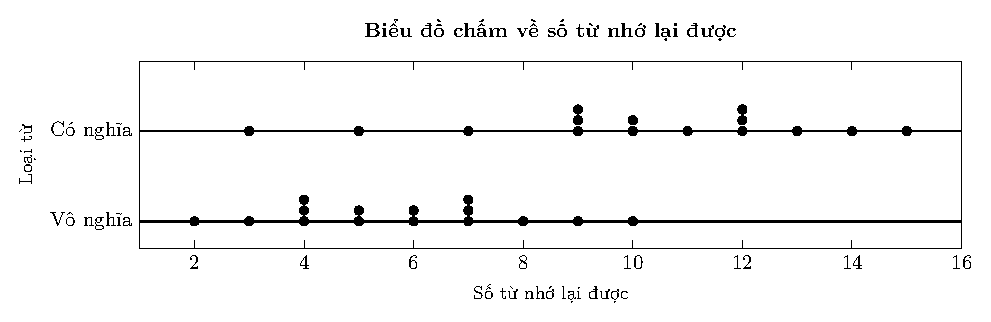
\includegraphics[width=.92\linewidth]{../figures/fhsm_2009_p75_1_vi.pdf}
\end{center}

\begin{scriptlist}
  \item [Giáo viên:] Nhìn vào các biểu đồ chấm, với loại từ nào thì học sinh nhìn chung có khả năng ghi nhớ tốt hơn? Em biết điều đó bằng cách nào? Hãy đưa ra những lý do cụ thể.
  \item [Học sinh A:]  Nhiều học sinh với danh sách từ có nghĩa làm tốt hơn. Số lớn nhất được nhớ lại ở nhóm từ vô nghĩa là mười. Có bảy học sinh trong nhóm từ có nghĩa nhớ được hơn mười từ, trong khi mười là kết quả cao nhất của toàn bộ nhóm từ vô nghĩa.
  \item [Học sinh B:] Đúng, nhưng cũng có một số học sinh với từ có nghĩa không làm tốt. Một bạn chỉ nhớ được ba từ; một bạn khác chỉ nhớ được năm từ; và một bạn nữa chỉ nhớ được bảy từ. Những giá trị này có vẻ thấp đối với nhóm từ có nghĩa.
  \item [Học sinh C:] Đúng vậy, và ở phía thấp của phân bố dữ liệu của nhóm từ có nghĩa có một số khoảng trống, trong khi phân bố của nhóm từ vô nghĩa thì không rõ điều đó. Nhiều học sinh với từ vô nghĩa nhớ được từ ba đến bảy từ, trong khi chỉ có rất ít học sinh với từ có nghĩa nằm trong khoảng này.
  \item [Giáo viên:] Em có thể nói cụ thể hơn không?
  \item [Học sinh C:]Vâng. Ba trong số mười lăm học sinh với từ có nghĩa nhớ được từ ba đến bảy từ, tức là chỉ $20$ phần trăm. Trong khi đó, ở nhóm từ vô nghĩa, mười một trên mười lăm học sinh, tức hơn $73$ phần trăm, nhớ được từng ấy từ. Nếu tính cả học sinh chỉ nhớ được hai từ vô nghĩa, thì mười hai trong số mười lăm học sinh, tức $80$ phần trăm, nhớ được từ hai đến bảy từ, trong khi chỉ có $20$ phần trăm học sinh với từ có nghĩa ở mức thấp như vậy. Thực tế, tất cả mười lăm học sinh với từ vô nghĩa đều nhớ được từ hai đến mười từ, trong khi chỉ có tám học sinh với từ có nghĩa ở mức thấp như vậy. 
  \item [Giáo viên:] Điều đó cũng giống như ý kiến của học sinh A: bảy trong số mười lăm học sinh dùng danh sách từ có nghĩa nhớ được nhiều từ hơn bất kỳ học sinh nào trong nhóm từ vô nghĩa. Điều này có nghĩa là gần một nửa số học sinh ghi nhớ từ có nghĩa làm tốt hơn toàn bộ nhóm từ vô nghĩa.
  \item [Giáo viên:] Bây giờ hãy thử xác định một giá trị điển hình cho số từ được nhớ lại của mỗi danh sách. Các em đề xuất dùng đại lượng nào?
  \item [Học sinh D:] Chúng ta có thể tính giá trị trung bình cho mỗi danh sách.
  \item [Giáo viên:] Tại sao em đề xuất dùng trung bình, hay còn gọi là số trung bình cộng?
  \item [Học sinh D:] Vì có vẻ như chúng ta luôn tìm trung bình mỗi khi muốn biết một giá trị điển hình.
  \item [Học sinh E:] Đúng là đôi khi trung bình tốt, nhưng đôi khi chúng ta lại dùng trung vị để biểu thị giá trị điển hình.
  \item [Giáo viên:] Trong trường hợp này, việc dùng cái nào có quan trọng không?
  \item [Học sinh E:] Với biểu đồ chấm của nhóm từ có nghĩa, ba giá trị trông khá nhỏ. Em nghĩ ba giá trị này có thể làm cho trung bình nhỏ hơn mức điển hình. Vì vậy em sẽ dùng trung vị thay vì trung bình.
  \item [Giáo viên:] Rất tốt. Khi quan sát một biểu đồ dữ liệu như biểu đồ chấm của nhóm từ có nghĩa, ta nói rằng dạng phân bố của dữ liệu bị lệch trái. Như học sinh E đã nói, khi phân bố dữ liệu lệch trái, trung bình thường nhỏ hơn giá trị mà ta xem là điển hình. Vì lý do này, trung vị có thể cho ta một chỉ báo tốt hơn về số từ mà học sinh với danh sách từ có nghĩa thường nhớ được. Vậy em sẽ đề xuất giá trị điển hình nào cho nhóm từ vô nghĩa?
  \item [Học sinh E:] Phân bố dữ liệu của nhóm từ vô nghĩa trông khá cân đối. Điều đó cho thấy nó có dạng đối xứng. Vì vậy, có lẽ ta có thể dùng cả trung bình lẫn trung vị. Nhưng vì chúng ta đang dùng trung vị cho nhóm từ có nghĩa, và sẽ không hợp lý nếu so sánh trung bình của nhóm này với trung vị của nhóm kia, nên em sẽ dùng trung vị cho nhóm từ vô nghĩa.
  \item [Giáo viên:] Các em khác nghĩ sao? Điều gì xảy ra khi chúng ta dùng trung vị?
  \item [Học sinh D:] Máy tính của em cho trung vị của nhóm từ có nghĩa là $10$, còn trung vị của nhóm từ vô nghĩa là $6$.
  \item [Giáo viên:] Nếu chúng ta không có các giá trị dữ liệu cụ thể, mà chỉ biết các trung vị, thì các trung vị cho ta biết điều gì về dữ liệu?
  \item [Học sinh D:] Trung vị chia dữ liệu thành hai nửa.
  \item [Giáo viên:] Đúng vậy. Vậy nếu trung vị là mười từ đối với dữ liệu từ có nghĩa, ta có thể nói gì về phần còn lại của dữ liệu?
  \item [Học sinh F:] Khoảng một nửa số học sinh với danh sách từ có nghĩa nhớ được ít hơn mười từ, và khoảng một nửa nhớ được nhiều hơn mười từ.
  \item [Giáo viên:] Khi so sánh hai trung vị, em rút ra kết luận gì?
  \item [Học sinh F:] Trung vị của nhóm từ có nghĩa là mười từ, còn trung vị của nhóm từ vô nghĩa là sáu từ. Mười lớn hơn sáu, nên học sinh với từ có nghĩa nhìn chung làm tốt hơn học sinh với từ vô nghĩa.
  \item [Giáo viên:]Đây là một nhận xét thú vị. Một cách khác để nhìn vào điều này là nói rằng sự chênh lệch giữa hai trung vị là bốn từ. Như vậy, học sinh với từ có nghĩa thường nhớ được nhiều hơn bốn từ so với học sinh với từ vô nghĩa.
  \item [Giáo viên:] Nếu chỉ báo cáo trung vị cho bộ dữ liệu này, thì thông tin gì về số từ được nhớ lại sẽ bị thiếu?
  \item [Học sinh G:] Nếu chỉ biết trung vị, ta không biết số từ cụ thể mà mỗi học sinh nhớ được. Ví dụ, trong dữ liệu của nhóm từ có nghĩa, nếu chỉ biết trung vị là mười từ, em không biết các giá trị khác thực sự đã xuất hiện như thế nào. Chẳng hạn, học sinh chỉ nhớ được ba từ khác xa rất nhiều so với mười từ.
  \item [Giáo viên:] Vậy học sinh G, ý tưởng mà em đang nói tới được gọi là gì?
  \item [Học sinh G:] Số từ được nhớ lại không giống nhau đối với mỗi học sinh. Em nghĩ đó chính là ý tưởng về sự biến thiên trong dữ liệu, điều mà chúng ta đã nói tới trước đây.
  \item [Giáo viên:] Đúng vậy. Trong thống kê, chúng ta quan tâm đến việc biểu diễn dữ liệu bằng một giá trị điển hình, chẳng hạn như trung vị, nhưng đồng thời cũng quan tâm đến việc tóm tắt mức độ biến thiên của dữ liệu. Có ai đề xuất cách làm điều đó không?
  \item [Học sinh H:] Chúng ta có thể tính khoảng biến thiên. Em nghĩ điều này cho biết phần nào mức độ biến thiên. Khoảng biến thiên của nhóm từ có nghĩa là $12$. Còn của nhóm từ vô nghĩa là $8$.
  \item [Giáo viên:] Vậy các khoảng biến thiên cho thấy điều gì về sự biến thiên trong dữ liệu?
  \item [Học sinh H:] Sự khác biệt lớn nhất giữa hai giá trị bất kỳ trong nhóm từ có nghĩa là mười hai từ, còn trong nhóm từ vô nghĩa là tám từ. Điều này cho thấy mức độ biến thiên trong số từ được nhớ lại ở nhóm từ có nghĩa lớn hơn so với nhóm từ vô nghĩa.
  \item [Học sinh I:] Nhưng giá trị nhỏ nhất của nhóm từ có nghĩa có vẻ rất thấp. Vì vậy em không nghĩ nên dùng khoảng biến thiên. Thay vào đó, em nghĩ chúng ta nên tìm các tứ phân vị và dùng khoảng tứ phân vị (IQR). Khi đó, em đang so sánh mức độ biến thiên của phần trung tâm trong mỗi nhóm.
  \item [Giáo viên:] Em tìm IQR như thế nào?
  \item [Học sinh I:] Trước hết phải tìm tứ phân vị thứ nhất và thứ ba cho mỗi nhóm dữ liệu. Sau đó lấy tứ phân vị thứ ba trừ đi tứ phân vị thứ nhất.
  \item [Giáo viên:] Được rồi. Mọi người hãy tìm các tứ phân vị và khoảng tứ phân vị.
  \item [Học sinh J:] Với nhóm từ có nghĩa, máy tính của em cho tứ phân vị thứ nhất là chín từ và tứ phân vị thứ ba là mười hai từ. Vậy IQR là ba từ. Với nhóm từ vô nghĩa, tứ phân vị thứ nhất là bốn từ và tứ phân vị thứ ba là bảy từ, nên IQR cũng là ba từ. Các IQR bằng nhau, nên mức độ biến thiên trong $50$ phần trăm dữ liệu trung tâm của hai nhóm là tương tự nhau.
  \item [Học sinh K:] Máy tính của em cho năm đại lượng cho mỗi nhóm: giá trị nhỏ nhất, tứ phân vị thứ nhất, trung vị, tứ phân vị thứ ba và giá trị lớn nhất. Em nghĩ từ năm số này chúng ta có thể vẽ một đồ thị gọi là biểu đồ hộp.
  \item [Giáo viên:] Đúng vậy. Khi kèm theo việc phân tích ngoại lệ, nó được gọi là biểu đồ hộp điều chỉnh.
\end{scriptlist}

Lớp học đã sử dụng kết quả từ máy tính để xây dựng các biểu đồ hộp điều chỉnh so sánh sau đây:

\begin{center}
  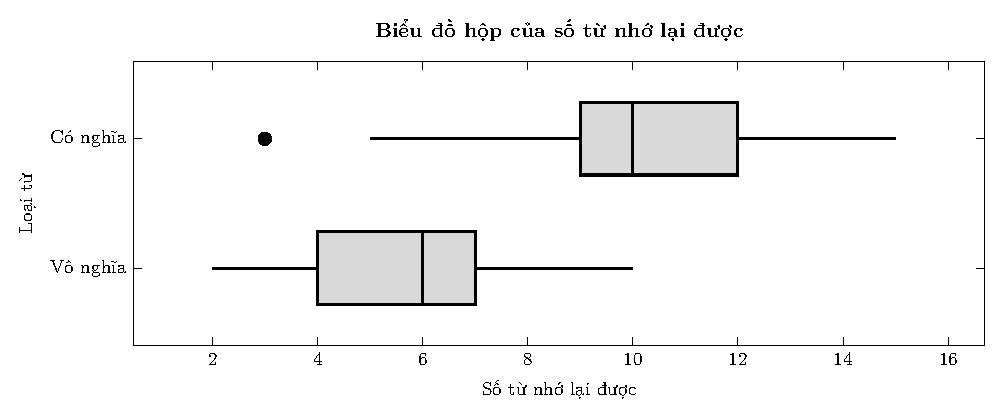
\includegraphics[width=.92\linewidth]{../figures/fhsm_2009_p79_1_vi.pdf}
\end{center}

\begin{scriptlist}
  \item [Giáo viên:] Các em có thể dùng kết quả từ các biểu đồ hộp để tóm tắt lại những thảo luận của chúng ta về câu hỏi này không?
  \item [Học sinh M:] Nhìn chung, học sinh với danh sách từ có nghĩa nhớ được nhiều từ hơn. Số từ tối đa được nhớ lại trong nhóm từ vô nghĩa là mười. Mười cũng chính là trung vị của nhóm từ có nghĩa, nên khoảng một nửa số học sinh với từ có nghĩa nhớ được nhiều từ hơn bất kỳ học sinh nào trong nhóm từ vô nghĩa. Trong nhóm từ có nghĩa, có một học sinh chỉ nhớ được ba từ; đây là một giá trị ngoại lệ và thấp hơn khá nhiều so với các dữ liệu còn lại. Trung vị của nhóm từ có nghĩa là mười, cao hơn bốn từ so với trung vị của nhóm từ vô nghĩa. Nếu loại bỏ ngoại lệ này khỏi dữ liệu của nhóm từ có nghĩa, thì hai nhóm có vẻ có mức độ biến thiên tương tự nhau. IQR của mỗi nhóm là $3$, cho thấy trong cả hai nhóm, số từ được nhớ lại trong $50$ phần trăm dữ liệu trung tâm chỉ khác nhau nhiều nhất là ba từ.
  \item [Giáo viên:] Những kết quả này gợi ý điều gì về trí nhớ và ý nghĩa?
  \item [Học sinh N:] Vì học sinh với các từ có nghĩa dường như làm tốt hơn, nên những dữ liệu này cho thấy việc ghi nhớ các từ có nghĩa là dễ hơn.
  \item [Giáo viên:] Các em có nghĩ rằng sẽ phù hợp nếu nói rằng tất cả học sinh lớp chín đều sẽ có kết quả giống hệt như vậy không?
  \item [Học sinh O:] Chắc chắn rồi, ghi nhớ từ có nghĩa thì dễ hơn.
  \item [Học sinh P:] Em nghĩ là chúng ta sẽ không có các điểm số y hệt! Nhưng có thể vẫn thấy rằng các từ có nghĩa sẽ dễ ghi nhớ hơn.
  \item [Giáo viên:] Chúng ta cần cẩn trọng về phạm vi suy luận, tức là việc khái quát các kết quả này cho các học sinh lớp chín khác dựa trên dữ liệu này. Phạm vi suy luận phụ thuộc vào việc lớp học được nghiên cứu có đại diện cho tất cả các lớp chín hay không. Vì chúng ta không biết lớp học này được chọn như thế nào, nên không nên khái quát kết quả cho tất cả các lớp chín hoặc cho toàn bộ học sinh lớp chín. Nếu một nhóm học sinh lớp chín được chọn ngẫu nhiên, khi đó ta mới có thể thử khái quát các kết quả này cho toàn bộ học sinh lớp chín.
  \item [Học sinh Q:] Nhưng em tưởng là họ đã dùng ngẫu nhiên trong nghiên cứu rồi?
  \item [Giáo viên:] Đúng là có dùng ngẫu nhiên. Tuy nhiên, ngẫu nhiên được sử dụng trong việc phân công học sinh vào các nhóm khác nhau. Mục đích của việc phân công ngẫu nhiên là tạo ra hai nhóm có thể so sánh được. Chẳng hạn, ta không muốn tất cả những học sinh có khả năng ghi nhớ tốt đều rơi vào cùng một nhóm. Bằng cách phân công ngẫu nhiên học sinh vào hai nhóm, ta hy vọng cân bằng được ảnh hưởng không chỉ từ khả năng ghi nhớ của học sinh mà còn từ bất kỳ biến nào khác có thể liên quan đến số từ được nhớ lại. Mặc dù phân công ngẫu nhiên không đảm bảo tạo ra các nhóm giống hệt nhau, nhưng nó làm tăng khả năng hình thành các nhóm tương tự nhau xét trên tất cả các biến.
\end{scriptlist}

\noindent
\textbf{Các yếu tố then chốt toán học}

Luận với thống kê và xác suất---Phân tích dữ liệu

\noindent
\textbf{Các thói quen luận}

Phân tích bài toán---quyết định liệu một cách tiếp cận thống kê có phù hợp hay không; xác định các khái niệm, thủ tục, hoặc biểu diễn toán học thích đáng; tìm kiếm các mẫu hình và quan hệ; đưa ra những suy diễn và phỏng đoán sơ bộ

Triển khai chiến lược---tổ chức lời giải  

Tìm kiếm và sử dụng các kết nối

Phản tư về lời giải---diễn giải lời giải; biện minh hoặc kiểm chứng một lời giải; nhận diện phạm vi suy luận
}
{}

\ParallelSection
  {Modeling Variability}
  {Mô hình hóa sự biến thiên}
  {}

\TriPara
{
\EN{Probability models reinforce the foundational principle that although an individual observation of a random variable cannot be predicted with certainty, patterns emerge in the frequency of values over a large number of observations. Fostering students' understanding of random variables and probability requires engaging them in the development of both simulation and mathematical probability models. The design of a simulation model requires that students set up a logical sequence of steps for describing the possible outcomes of a random variable. The implementation of a simulation model allows students to both experience and make sense of the notion of the long-run behavior of a random variable and to determine experimental probabilities. The design and implementation of a simulation also provides transitional steps in the development of reasonable mathematical models for describing the long-run behavior of a random variable. Because many probability models involve counting, probability has connections with the Numbers and Measurements strand and the key element of counting described in chapter 4. Example 20 considers various developmental strategies for arriving at a solution to a probability problem and illustrates the importance of identifying relevant concepts, procedures, or representations and knowing how a solution can be generalized to a broader class of problems.}
}
{
\VI{Các mô hình xác suất củng cố nguyên lý nền tảng rằng, mặc dù không thể dự đoán chắc chắn một quan sát riêng lẻ của một biến ngẫu nhiên, nhưng các khuôn mẫu sẽ xuất hiện trong tần suất của các giá trị khi số lượng quan sát đủ lớn. Việc bồi dưỡng cho học sinh sự hiểu biết về biến ngẫu nhiên và xác suất đòi hỏi phải lôi cuốn các em tham gia vào quá trình xây dựng cả các mô hình xác suất mô phỏng lẫn các mô hình xác suất toán học. Thiết kế một mô hình mô phỏng yêu cầu học sinh thiết lập một chuỗi các bước hợp lý để mô tả các kết quả có thể xảy ra của một biến ngẫu nhiên. Việc triển khai mô hình mô phỏng cho phép học sinh vừa trải nghiệm vừa tạo lập ý nghĩa cho khái niệm hành vi dài hạn của một biến ngẫu nhiên, đồng thời xác định các xác suất thực nghiệm. Quá trình thiết kế và triển khai mô phỏng cũng cung cấp những bước chuyển tiếp trong việc phát triển các mô hình toán học hợp lý nhằm mô tả hành vi dài hạn của một biến ngẫu nhiên. Vì nhiều mô hình xác suất liên quan đến việc đếm, nên xác suất có mối liên hệ với mạch \emph{số và đo lường} và yếu tố cốt lõi \emph{đếm} được trình bày trong Chương 4. Ví dụ 20 xem xét nhiều chiến lược phát triển khác nhau để đi tới lời giải của một bài toán xác suất, đồng thời minh họa tầm quan trọng của việc xác định các khái niệm, quy trình hoặc biểu diễn liên quan và hiểu được cách một lời giải có thể được khái quát hóa cho một lớp bài toán rộng hơn.}
}
{
\NOTE{}
}

\TriExample
{What Are the Chances? Part A}
{
\noindent
\textbf{Task}

A high school club has fifty members: ten girls and forty boys. The refreshments committee will be formed by selecting two students from the club at random. What is the probability of getting exactly zero girls on the committee? Exactly one girl on the committee? Exactly two girls on the committee? That is, if two students are repeatedly selected at random from the club, how often will exactly no girl be selected? Exactly one girl? Exactly two girls?

\noindent
\textbf{In the Classroom (Ninth- to Twelfth-Grade Mathematics Classes)}

The class is instructed to design a hands-on simulation for estimating the probability for each of the different possible results for the number of girls on the committee. Prior to this activity, students should have had experiences performing simulations by using various random devices and random-number generators in graphing calculators. After the task is read, the teacher can ask the students how they might design a simulation for the situation of choosing two students for the committee and reporting the number of girls on the
committee.

The teacher can lead a discussion to help students design the simulation. Students may propose the use of a standard deck of cards (they would remove two face cards and represent the girls with the ten remaining face cards and the boys with the forty non-face cards). For each trial, they would shuffle the deck several times and then select two cards. The number of face cards selected represents the number of girls on the committee. For the next trial, they would replace the cards in the deck, reshuffle, and select two more cards. Students would need to decide how many trials to perform. From previous experiences, students know that the relative frequencies tend to be close to the actual probabilities if they perform a large number of trials. Together, the class performed a simulation of two hundred trials. The results are summarized in the table at the top of the next page.

\begin{center}
\begin{tabular}{|
>{\centering\arraybackslash}m{1.8cm}|
>{\centering\arraybackslash}m{1.8cm}|
>{\centering\arraybackslash}m{3.0cm}|}
\hline
Number of Girls & Frequency & Experimental Probability \\
\hline
$0$ & $121$ & $.605$ \\
\hline
$1$ & $70$  & $.350$ \\
\hline
$2$ & $9$   & $.045$ \\
\hline
    & $200$ & $1.000$ \\
\hline
\end{tabular}
\end{center}

The experimental probabilities provide estimates for the true probabilities for each of the different possible results and illustrate the long-run relative frequency interpretation of probability.

\noindent
\textbf{In the Classroom (High School Statistics Class)}

Students can revisit this problem in a statistics class after they have learned about tree diagrams and are learning about rules of probability. The class constructed the tree diagram at the right for describing the gender of the two students selected.

\begin{center}
  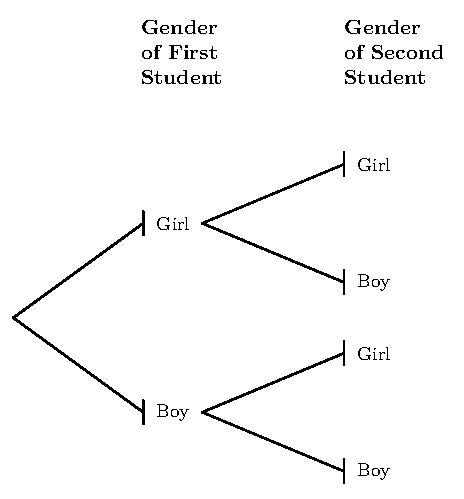
\includegraphics[width=.92\linewidth]{../figures/fhsm_2009_p82_1.pdf}
\end{center}

Students are asked to describe the ordered sequence of outcomes for gender that results in the number of girls selected to be 0. For this outcome, the ordered sequence must be---

\begin{quote}
  Boy selected first and boy selected second.
\end{quote}

Students are asked to determine the probability that the first student selected is a boy, which they all agree is

$$
  \frac{40}{50},
$$

or $0.8$.

They are then asked to think about the probability that the second student selected is a boy, and many said

$$
  \frac{39}{49}.
$$

The teacher asks about any assumptions made in determining this probability, and the class agrees that this probability assumes that the first student selected is a boy. The teacher points out that

$$
  \frac{39}{49}
$$

is called a “conditional” probability and represents the probability that the second student selected is a boy, given that the first student selected is a boy. The teacher then asks about the probability of the ordered sequence “Boy selected first and boy selected second.” A student responds that the sequence can occur only if a boy is selected first and, given that a boy was selected first, a boy is selected second. That is,

\begin{align*}
  P(0\, \text{Girls})
    &= P\left(\text{\parbox{5cm}{Boy selected first and Boy selected second}}\right)\\
    &= P(\text{Boy selected first})\cdot\\
      &\qquad P\left(\text{\parbox{5cm}{Boy selected second given Boy selected first}}\right) \\
    &= \frac{40}{50}\cdot\frac{39}{49}.
\end{align*}

The teacher uses this opportunity to present the product rule for probability:

\begin{align*}
  P&(A\, \text{and}\, B)\\
    &= P(A)P(\text{$B$ given that $A$ has occurred}).
\end{align*}

The class expands the tree diagram to show the conditional probabilities for the outcome of gender at each stage of the selection, the ordered sequence of gender, and the number of girls selected for each ordered sequence.

\begin{center}
  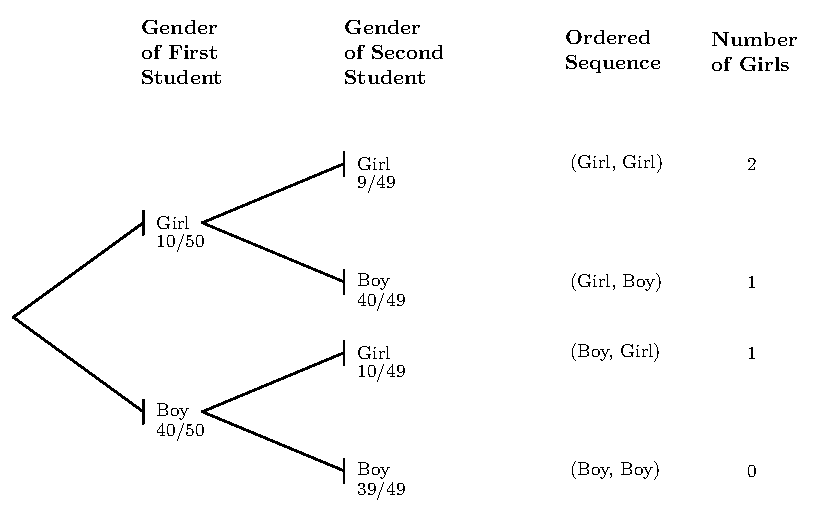
\includegraphics[width=.92\linewidth]{../figures/fhsm_2009_p83_1.pdf}
\end{center}

By traversing the tree and using the product rule, the class determines each of the following probabilities:

\begin{align*}
  P(\text{No Girls})&=(40/50)(39/49)\\
    &\approx .637, \\
  P(\text{One Girl})&=(10/50)(40/49)+(40/50)(10/49)\\
    & \approx .327, \, \text{and} \\
  P(\text{Two Girls})&=P(\text{Girl on First and Girl on Second})\\
    &=(10/50)(9/49)\\
    & \approx .037.
\end{align*}

The teacher then asks the class to think about the following question for homework.

\begin{quote}
  Suppose the gender of the first student selected is not known. We are interested in knowing the probability that the second student selected is a girl (regardless of the gender of the first student selected). This probability is---

  $$ 
  P(\text{Girl selected Second}) =\frac{10}{50}.
  $$

  Can you explain why this is the probability?
\end{quote}

\noindent
\textbf{In the Classroom (Twelfth Grade)}

Students can revisit this problem in the twelfth grade after they have learned counting rules. The class is instructed to use counting rules for determining the probability for each of the different possible results for the number of girls on the committee and to interpret the probabilities. Revisiting the same problem at a higher level gives students an opportunity to make sense of their earlier simulation.

Students are reminded that

$$
  C(m,k)=\frac{m!}{k!(m-k)!}
$$

counts the number of subsets of size $k$ from $m$ distinct objects.

For this problem, we get $C(50, 2)$, or $1225$, possible subsets (committees) of size two from the club of fifty students. Since the selection is random, we can assume that each possible committee is equally likely. The number of committees with---

\begin{quote}
  exactly $0$ girls (and exactly $2$ boys) is $C(10, 0) \cdot C(40, 2)$, or $780$;

  exactly $1$ girl (and exactly $1$ boy) is $C(10, 1) \cdot C(40, 1)$, or $400$;

  exactly $2$ girls (and exactly $0$ boys) is $C(10, 2) \cdot C(40, 0)$, or $45$.
\end{quote}

Thus, the mathematical probabilities are as shown in the following table:

\begin{center}
\begin{tabular}{|c|c|}
\hline
Number of Girls & Probability \\
\hline
$0$ & $\frac{780}{1225}\approx .637$ \\
\hline
$1$ & $\frac{400}{1225}\approx .327$ \\
\hline
$2$ & $\frac{45}{1225}\approx .037$ \\
\hline
\end{tabular}
\end{center}

This example can be used as a rationale for developing the general formula for calculating these types of probabilities when sampling from a fi nite population. Suppose you have a population with $N$ objects and each object is classified as either a success or a failure. Within the population, $M$ of the objects are successes. You plan to randomly select $n$ objects and to count the number of successes among those selected. For this situation, the number of successes is called a \emph{hypergeometric random variable}, and the probability of obtaining exactly $x$ successes is given by

$$
  P(x)=\frac{C(M,x)\cdot C(N-M,n-x)}{C(N,n)}.
$$

\noindent
\textbf{\emph{Summary of example 20}}

Note that the estimated probabilities from the simulation in the first task are close to the probabilities obtained either through counting or using the tree diagram. These latter probabilities indicate that if two members are repeatedly selected at random from the club, then on any one trial, getting exactly zero girls is most likely and would occur approximately $64$ percent of the time. Getting exactly one girl on the committee is fairly common and would occur approximately $33$ percent of the time. In addition, since the probability of getting exactly two girls is less than $.04$, it would be unusual for the committee to have two girls. An examination of this problem from a statistical perspective is described in example 21.

\noindent
\textbf{Key Elements of Mathematics}

Reasoning with Statistics and Probability---Modeling variability

Number and Measurement---Counting

\noindent
\textbf{Reasoning Habits}

Analyzing a problem---identifying relevant concepts, procedures, or representations

Implementing a strategy---making logical deductions

Seeking and using connections

Reflecting on one's solution---interpreting a solution; generalizing a solution
}
{Bao nhiêu khả năng? Part A}
{
\noindent
\textbf{Nhiệm vụ}

Một câu lạc bộ trung học phổ thông có năm mươi thành viên: mười bạn nữ và bốn mươi bạn nam. Ban phụ trách nước uống sẽ được lập bằng cách chọn ngẫu nhiên hai học sinh từ câu lạc bộ. Xác suất để ban này có đúng không bạn nữ là bao nhiêu? Có đúng một bạn nữ là bao nhiêu? Có đúng hai bạn nữ là bao nhiêu? Nói cách khác, nếu hai học sinh được chọn ngẫu nhiên lặp đi lặp lại từ câu lạc bộ, thì sẽ có bao nhiêu lần đúng là không có nữ sinh nào được chọn? Đúng một nữ sinh? Đúng hai nữ sinh?

\noindent
\textbf{Trong lớp học (Lớp Toán từ lớp 9 đến lớp 12)}

Lớp được hướng dẫn thiết kế một mô phỏng thực hành để ước lượng xác suất cho từng kết quả có thể xảy ra về số bạn nữ trong ban phụ trách. Trước hoạt động này, học sinh cần đã có trải nghiệm thực hiện mô phỏng bằng nhiều thiết bị ngẫu nhiên khác nhau và bằng các bộ sinh số ngẫu nhiên trong máy tính cầm tay vẽ đồ thị. Sau khi đọc đề bài, giáo viên có thể hỏi học sinh rằng các em có thể thiết kế một mô phỏng cho tình huống chọn hai học sinh vào ban phụ trách và báo cáo số bạn nữ trong ban như thế nào.

Giáo viên có thể dẫn dắt thảo luận để giúp học sinh thiết kế mô phỏng. Học sinh có thể đề xuất sử dụng một bộ bài tiêu chuẩn (các em sẽ bỏ đi hai lá hình, rồi dùng mười lá hình còn lại để biểu diễn các bạn nữ và bốn mươi lá không hình để biểu diễn các bạn nam). Ở mỗi lần thử, các em sẽ xáo bài vài lần rồi rút hai lá. Số lá hình được rút ra biểu diễn số bạn nữ trong ban phụ trách. Đến lần thử tiếp theo, các em trả lại các lá bài vào bộ, xáo lại, rồi rút thêm hai lá. Học sinh cần quyết định sẽ thực hiện bao nhiêu lần thử. Từ những kinh nghiệm trước đó, học sinh biết rằng các tần suất tương đối thường gần với các xác suất thực nếu các em thực hiện một số lượng lớn lần thử. Cả lớp đã cùng nhau thực hiện một mô phỏng gồm hai trăm lần thử. Kết quả được tóm tắt trong bảng ở đầu trang kế tiếp.

\begin{center}
\begin{tabular}{|
>{\centering\arraybackslash}m{1.8cm}|
>{\centering\arraybackslash}m{1.8cm}|
>{\centering\arraybackslash}m{3.0cm}|}
\hline
Số nữ & Tần số & \shortstack{Xác suất\\thực nghiệm} \\
\hline
$0$ & $121$ & $.605$ \\
\hline
$1$ & $70$  & $.350$ \\
\hline
$2$ & $9$   & $.045$ \\
\hline
    & $200$ & $1.000$ \\
\hline
\end{tabular}
\end{center}

Các xác suất thực nghiệm cung cấp những ước lượng cho các xác suất thực đối với từng kết quả có thể xảy ra, đồng thời minh họa cách diễn giải xác suất theo tần số tương đối trong dài hạn.

\noindent
\textbf{Trong lớp học (Lớp Thống kê trung học phổ thông)}

Học sinh có thể quay lại bài toán này trong lớp thống kê sau khi đã học về sơ đồ cây và đang học về các quy tắc xác suất. Cả lớp đã xây dựng sơ đồ cây ở bên dưới để mô tả giới tính của hai học sinh được chọn.

\begin{center}
  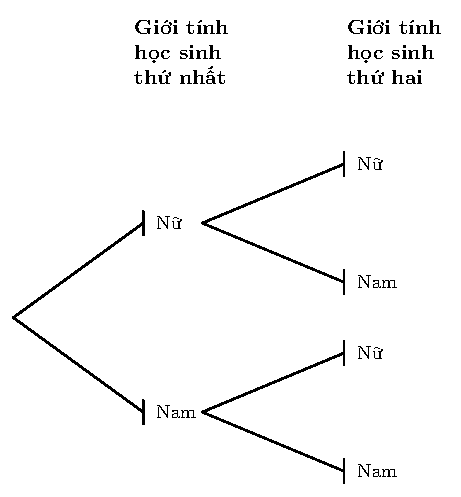
\includegraphics[width=.92\linewidth]{../figures/fhsm_2009_p82_1_vi.pdf}
\end{center}

Học sinh được yêu cầu mô tả chuỗi kết quả có thứ tự về giới tính sao cho số bạn nữ được chọn là $0$. Với kết quả này, chuỗi có thứ tự phải là---

\begin{quote}
  Chọn nam ở lượt thứ nhất và chọn nam ở lượt thứ hai.
\end{quote}

Học sinh được yêu cầu xác định xác suất để học sinh thứ nhất được chọn là nam; cả lớp đều đồng ý rằng đó là

$$
  \frac{40}{50},
$$

hay $0.8$.

Sau đó, học sinh được yêu cầu suy nghĩ về xác suất để học sinh thứ hai được chọn là nam, và nhiều em trả lời là

$$
  \frac{39}{49}.
$$

Giáo viên hỏi các em đã đưa ra giả định nào khi xác định xác suất này, và cả lớp đồng ý rằng xác suất đó giả định học sinh thứ nhất được chọn là nam. Giáo viên chỉ ra rằng

$$
  \frac{39}{49}
$$

được gọi là một xác suất ``có điều kiện'' và biểu thị xác suất để học sinh thứ hai được chọn là nam, với điều kiện học sinh thứ nhất đã được chọn là nam. Sau đó, giáo viên hỏi về xác suất của chuỗi có thứ tự ``chọn nam ở lượt thứ nhất và chọn nam ở lượt thứ hai''. Một học sinh trả lời rằng chuỗi này chỉ có thể xảy ra nếu chọn nam ở lượt thứ nhất và, với điều kiện đã chọn nam ở lượt thứ nhất, chọn nam ở lượt thứ hai. Tức là,

\begin{align*}
  P(0 \, \text{nữ})
    &= P\left(\text{\parbox{5cm}{Nam được chọn ở lượt 1 và nam được chọn ở lượt 2}}\right)\\
    &= P\left(\text{Nam được chọn ở lượt 1}\right)\cdot\\
      &\qquad P\left(\text{\parbox{5cm}{Nam được chọn ở lượt 2 khi nam đã được chọn ở lượt 1}}\right) \\
    &= \frac{40}{50}\cdot\frac{39}{49}.
\end{align*}

Giáo viên nhân cơ hội này giới thiệu quy tắc nhân của xác suất:

\begin{align*}
  P&(A\, \text{và}\, B)\\
    &= P(A)P(\text{$B$ với điều kiện $A$ đã xảy ra}).
\end{align*}

Cả lớp mở rộng sơ đồ cây để thể hiện các xác suất có điều kiện cho kết quả về giới tính ở mỗi giai đoạn chọn, chuỗi giới tính có thứ tự, và số bạn nữ được chọn ứng với mỗi chuỗi.

\begin{center}
  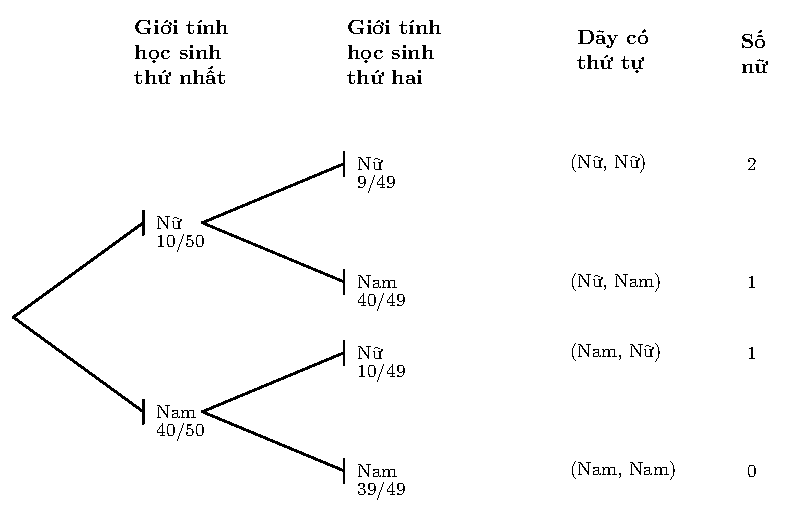
\includegraphics[width=.92\linewidth]{../figures/fhsm_2009_p83_1_vi.pdf}
\end{center}

Bằng cách lần theo sơ đồ cây và sử dụng quy tắc nhân, cả lớp xác định từng xác suất sau đây:

\begin{align*}
  P(\text{Không nữ})
    &=(40/50)(39/49)\\ 
    &\approx .637,\\
  P(\text{Một nữ})
    &=(10/50)(40/49)+(40/50)(10/49)\\
    &\approx .327, \,\text{và} \\
  P(\text{Hai nữ})
    &=P(\text{Nữ ở lượt 1 và nữ ở lượt 2})\\
    &=(10/50)(9/49)\\
    &\approx .037.
\end{align*}

Sau đó, giáo viên yêu cầu học sinh suy nghĩ câu hỏi sau như một bài tập về nhà:

\begin{quote}
  Giả sử giới tính của học sinh được chọn ở lượt thứ nhất không được biết. Ta quan tâm đến xác suất để học sinh được chọn ở lượt thứ hai là nữ (không phụ thuộc giới tính của học sinh lượt thứ nhất). Xác suất này là

  $$
  P(\text{Nữ được chọn ở lượt 2})
    =\frac{10}{50}.
  $$

  Em có thể giải thích vì sao đây là xác suất đúng không?
\end{quote}

\noindent
\textbf{Trong lớp học (Lớp 12)}

Học sinh có thể quay lại bài toán này ở lớp 12 sau khi đã học các quy tắc đếm. Lớp được hướng dẫn sử dụng các quy tắc đếm để xác định xác suất cho từng kết quả có thể xảy ra về số bạn nữ trong ban phụ trách, đồng thời diễn giải các xác suất đó. Việc xem lại cùng một bài toán ở mức độ cao hơn tạo cơ hội cho học sinh tạo lập ý nghĩa đối với mô phỏng mà các em đã thực hiện trước đó.

Học sinh được nhắc rằng

$$
  C(m,k)=\frac{m!}{k!(m-k)!}
$$

đếm số tập con có kích thước $k$ được chọn từ $m$ phần tử phân biệt.

Trong bài toán này, ta có $C(50,2)$, tức $1225$, tập con (ban) có kích thước hai được chọn từ câu lạc bộ năm mươi học sinh. Vì việc chọn là ngẫu nhiên, ta có thể giả sử rằng mỗi ban có khả năng được chọn như nhau. Số ban có---

\begin{quote}
  đúng $0$ bạn nữ (và đúng $2$ bạn nam) là $C(10,0)\cdot C(40,2)$, tức $780$;

  đúng $1$ bạn nữ (và đúng $1$ bạn nam) là $C(10,1)\cdot C(40,1)$, tức $400$;

  đúng $2$ bạn nữ (và đúng $0$ bạn nam) là $C(10,2)\cdot C(40,0)$, tức $45$.
\end{quote}

Vì vậy, các xác suất toán học được trình bày trong bảng sau:

\begin{center}
\begin{tabular}{|c|c|}
\hline
Số nữ & xác suất \\
\hline
$0$ & $\frac{780}{1225}\approx .637$ \\
\hline
$1$ & $\frac{400}{1225}\approx .327$ \\
\hline
$2$ & $\frac{45}{1225}\approx .037$ \\
\hline
\end{tabular}
\end{center}

Ví dụ này có thể được dùng như một cơ sở để phát triển công thức tổng quát nhằm tính các xác suất kiểu này khi lấy mẫu từ một quần thể hữu hạn. Giả sử ta có một quần thể gồm $N$ đối tượng và mỗi đối tượng được phân loại là ``thành công'' hoặc ``thất bại''. Trong quần thể đó, có $M$ đối tượng là ``thành công''. Ta dự định chọn ngẫu nhiên $n$ đối tượng và đếm số ``thành công'' trong số các đối tượng được chọn. Trong tình huống này, số ``thành công'' được gọi là một \emph{biến ngẫu nhiên siêu bội}, và xác suất để thu được đúng $x$ ``thành công'' được cho bởi

$$
  P(x)=\frac{C(M,x)\cdot C(N-M,n-x)}{C(N,n)}.
$$

\noindent
\textbf{\emph{Tóm tắt Ví dụ 20}}

Lưu ý rằng các xác suất ước lượng từ mô phỏng trong nhiệm vụ đầu tiên gần với các xác suất thu được bằng cách đếm hoặc sử dụng sơ đồ cây. Các xác suất sau này cho thấy rằng nếu hai thành viên được chọn ngẫu nhiên lặp đi lặp lại từ câu lạc bộ, thì trong một lần chọn bất kỳ, việc có đúng không bạn nữ là khả dĩ nhất và sẽ xảy ra xấp xỉ $64$ phần trăm số lần. Việc có đúng một bạn nữ trong ban là khá phổ biến và sẽ xảy ra xấp xỉ $33$ phần trăm số lần. Ngoài ra, vì xác suất có đúng hai bạn nữ nhỏ hơn $0.04$ nên việc ban có hai bạn nữ là một trường hợp không thường gặp. Việc xem xét bài toán này từ góc nhìn thống kê được trình bày trong Ví dụ 21.

\noindent
\textbf{Các yếu tố then chốt toán học}

Luận với thống kê và xác suất---Mô hình hóa biến thiên  

Luận với số và đo lường---Đếm

\noindent
\textbf{Các thói quen luận}

Phân tích bài toán---xác định các khái niệm, thủ tục, hoặc biểu diễn toán học thích đáng  

Triển khai chiến lược---thực hiện những suy diễn có tính luận lý

Tìm kiếm và sử dụng các kết nối  

Phản tư về lời giải---diễn giải lời giải; khái quát hóa lời giải
}
{
Ví dụ 20 được thiết kế như một tiến trình nhiều tầng, nhằm làm nổi bật cách luận xác suất được xây dựng dần từ trực giác đến hình thức. Cùng một bài toán được nhìn qua ba lăng kính: mô phỏng thực nghiệm, mô hình hóa bằng sơ đồ cây với xác suất có điều kiện và quy tắc nhân, rồi quy tắc đếm ở mức độ cao hơn.

Phần mô phỏng nhấn mạnh cách hiểu xác suất theo tần suất trong dài hạn. Việc yêu cầu học sinh thiết kế phép mô phỏng buộc các em phải mô hình hóa tình huống: quyết định cách mã hóa, chọn thiết bị ngẫu nhiên, quyết định số lần thử, và hiểu vì sao khi số lần thử đủ lớn thì tần suất có xu hướng tiến gần xác suất thực.

Phần sơ đồ cây đưa học sinh từ trải nghiệm sang cấu trúc. Sự xuất hiện của xác suất có điều kiện ở đây không phải là một công thức được cho sẵn, mà là hệ quả tự nhiên của việc rút không hoàn lại. Qua đó, học sinh thấy rõ vì sao quy tắc nhân là cần thiết khi các bước chọn không độc lập với nhau.

Phần lớp 12 đưa vào quy tắc đếm và mở ra sự khái quát hóa ở trường hợp siêu bội. Đây là một bước quan trọng: thay vì chỉ giải một bài toán riêng lẻ, học sinh được dẫn đến một khuôn mẫu tổng quát cho việc lấy mẫu từ một quần thể hữu hạn, từ đó đặt nền cho tư duy mô hình và suy luận thống kê.

\vspace{0.3\baselineskip}
\noindent
\textbf{Ghi chú về có thứ tự và không}

Trong Ví dụ 20, việc xét thứ tự chọn học sinh không nhằm thay đổi bản chất của bài toán, vì điều bài toán quan tâm rốt cuộc vẫn là số nữ sinh trong ban. Việc đưa thứ tự vào nhằm làm nổi bật cấu trúc của một quá trình ngẫu nhiên nhiều bước. Nhờ đó, xác suất có điều kiện và quy tắc nhân có thể xuất hiện một cách tự nhiên, trước khi học sinh chuyển sang cách tiếp cận không xét thứ tự bằng các quy tắc đếm ở lớp 12.

\begin{quote}
  Nhưng có phải xét đến thứ tự là làm sai bản chất của bài toán?
\end{quote}

\vspace{0.3\baselineskip}
\noindent
\emph{Không}. Vì:

\begin{itemize}
  \item Mỗi ban không có thứ tự tương ứng với hai chuỗi có thứ tự: $(\text{nam}, \text{nữ}) \leftrightarrow (\text{nữ}, \text{nam})$.
  \item Khi cộng hai xác suất có thứ tự ấy, ta trở lại đúng xác suất của ban có $1$ nữ:

  $$
  \frac{10}{50}\cdot\frac{40}{49}+\frac{40}{50}\cdot\frac{10}{49}
  = \frac{C(10,1)\cdot C(40,1)}{C(50,2)}.
  $$
\end{itemize}

\noindent
Nói cách khác, việc xét theo thứ tự không làm đổi bài toán; nó chỉ biểu diễn bài toán dưới một dạng thuận lợi hơn để làm lộ ra cấu trúc xác suất của quá trình chọn.

\vspace{0.3\baselineskip}
\noindent
\textbf{Ghi chú về công thức nhân $P(A\cap B)=P(A)P(B\mid A)$}

Về mặt trực giác, ta dùng phép nhân trong công thức

$$
P(A\cap B)=P(A)P(B\mid A)
$$

vì sự kiện ``$A$ và $B$'' ở đây được hiểu như một quá trình gồm hai bước liên tiếp: trước hết rơi vào $A$, rồi trong điều kiện $A$ đã xảy ra, tiếp tục rơi vào $B$. Xác suất của toàn bộ quá trình vì thế bằng tỉ lệ đi qua được bước thứ nhất nhân với tỉ lệ đi qua được bước thứ hai. Phép nhân ở đây không phải là một quy ước áp đặt từ bên ngoài, mà là hệ quả trực tiếp của cách hiểu cấu trúc của ``và'' trong một quá trình xác suất nhiều bước.

Về mặt toán học, xác suất có điều kiện được lấy làm định nghĩa, và công thức nhân là hệ quả trực tiếp của định nghĩa ấy. Tuy nhiên, trong dạy học, người ta thường dẫn dắt học sinh đến công thức nhân thông qua các quá trình nhiều bước và sơ đồ cây, rồi sau đó mới giới thiệu khái niệm xác suất có điều kiện để hợp thức hóa điều mà trực giác đã nắm được.

Trong hệ thống Kolmogorov, xác suất có điều kiện không phải là một tiên đề mà là một định nghĩa. Nó không đặt thêm một ràng buộc mới lên xác suất, mà chỉ đặt tên cho một biểu thức đã được xác định từ khuôn khổ tiên đề của độ đo xác suất. Vì vậy, công thức xác suất có điều kiện không được gọi là tiên đề, dù nó giữ vai trò nền tảng trong suy luận xác suất.
}

\ParallelSection
  {Connecting Statistics and Probability}
  {Kết nối Thống kê và Xác suất}
  {}

\TriPara
{
\EN{By incorporating randomness into data collection, probability provides a way to make sense of the variation in sample results from one sample to another. The sampling distribution of a sample statistic (e.g., the sample mean, the sample median, the number of successes or the proportion of successes in the sample) summarizes the long-run behavior of the statistic from repeated random sampling. The sampling distribution provides a mechanism for describing the variation expected in a sample statistic and for determining whether an observed value might be reasonable from chance variation or whether it is more likely due to some other factor. The activity “Sampling Rectangles” in \emph{Navigating through Data Analysis in Grades 9--12} (Burrill et al. 2003) illustrates important ideas related to the sampling distribution of the sample mean. The probability distribution developed in example 20 represents the sampling distribution for the number of girls (successes) in a random sample of size two selected from a club of fifty students with ten girls and forty boys. Sampling distributions make crucial links among data analysis, probability, and inferential reasoning in statistics. The following example illustrates foundational ideas underlying the reasoning in inferential statistics by considering the reasonableness of a solution and revisiting initial assumptions.}
}
{
\VI{Bằng cách đưa yếu tố ngẫu nhiên vào việc thu thập dữ liệu, xác suất cung cấp một cách để hiểu sự biến thiên của các kết quả mẫu từ mẫu này sang mẫu khác. Phân phối lấy mẫu của một thống kê mẫu, chẳng hạn trung bình mẫu, trung vị mẫu, số lần thành công, hay tỉ lệ thành công trong mẫu, tóm lược hành vi dài hạn của thống kê ấy qua việc lấy mẫu ngẫu nhiên lặp đi lặp lại. Phân phối lấy mẫu cung cấp một cơ chế để mô tả mức biến thiên có thể được chờ đợi ở một thống kê mẫu, đồng thời để xác định xem một giá trị quan sát được có thể được xem là hợp lí do biến thiên ngẫu nhiên hay nhiều khả năng là do một nhân tố khác. Hoạt động “Sampling Rectangles” trong *Navigating through Data Analysis in Grades 9--12* (Burrill et al. 2003) minh họa những ý tưởng quan trọng liên quan đến phân phối lấy mẫu của trung bình mẫu. Phân phối xác suất được xây dựng trong Ví dụ 20 biểu diễn phân phối lấy mẫu của số học sinh nữ, tức số lần thành công, trong một mẫu ngẫu nhiên cỡ hai được chọn từ một câu lạc bộ gồm năm mươi học sinh, trong đó có mười nữ và bốn mươi nam. Các phân phối lấy mẫu tạo ra những mối nối then chốt giữa phân tích dữ liệu, xác suất, và suy luận thống kê. Ví dụ tiếp theo minh họa những ý tưởng nền tảng nằm dưới lối luận trong suy luận thống kê, thông qua việc xét tính hợp lí của một lời giải và xem xét lại những giả định ban đầu.}
}
{
\NOTE{Sự khó hiểu trước hết nằm ở chỗ có quá nhiều tầng đối tượng chồng lên nhau: dữ liệu, mẫu, thống kê mẫu, xác suất, rồi phân phối lấy mẫu. Muốn đọc đoạn văn này cho sáng, cần tách các tầng ấy ra.

Khi chỉ nhìn vào một mẫu cụ thể, chẳng hạn lấy ngẫu nhiên hai học sinh trong một câu lạc bộ rồi đếm số học sinh nữ, kết quả thu được chỉ là một giá trị. Nhưng nếu hình dung việc lấy mẫu ấy được lặp đi lặp lại rất nhiều lần, thì số học sinh nữ trong mẫu sẽ không luôn giống nhau. Có lúc là $0$, có lúc là $1$, có lúc là $2$. Sự thay đổi ấy chính là biến thiên từ mẫu này sang mẫu khác.

Xác suất được đưa vào để mô tả biến thiên đó. Nó cho phép không chỉ nói rằng các kết quả khác nhau có thể xảy ra, mà còn nói mỗi kết quả có khả năng xảy ra đến mức nào. Khi đó, thay vì chỉ có một kết quả mẫu đơn lẻ, ta có cả một bức tranh về tất cả những kết quả có thể xuất hiện cùng với khả năng của chúng. Bức tranh ấy là phân phối lấy mẫu.

Vì vậy, phân phối lấy mẫu không phải là phân phối của từng cá nhân trong quần thể, cũng không phải là phân phối của toàn bộ dữ liệu gốc. Nó là phân phối của một đại lượng được tính từ mẫu. Đại lượng ấy có thể là trung bình mẫu, trung vị mẫu, số lần thành công, hay tỉ lệ thành công. Nói ngắn gọn, phân phối lấy mẫu mô tả một thống kê mẫu sẽ biến động ra sao nếu việc lấy mẫu ngẫu nhiên được lặp lại nhiều lần.

Chỗ then chốt nằm ở đây: một giá trị quan sát được từ mẫu chỉ thật sự có ý nghĩa khi được đặt vào bối cảnh của phân phối lấy mẫu. Nếu một giá trị nằm trong vùng thường gặp của phân phối ấy, thì nó có thể được xem là hợp lí do biến thiên ngẫu nhiên. Nếu nó rơi vào vùng rất hiếm, thì cần nghĩ đến khả năng có một nguyên nhân khác, chứ không chỉ do ngẫu nhiên.

Ví dụ 20 được nhắc tới để làm đúng bước nối đó. Trong ví dụ ấy, xác suất không còn đứng riêng như một bài toán đếm thuần túy, mà trở thành công cụ mô tả số học sinh nữ trong một mẫu ngẫu nhiên cỡ hai. Nhờ vậy, xác suất bắt đầu gắn trực tiếp với một kết quả thống kê có thể quan sát được từ mẫu. Đó chính là chỗ nối giữa phân tích dữ liệu và suy luận thống kê.

Điểm sâu hơn là: suy luận thống kê không bắt đầu từ việc “kết luận ngay từ dữ liệu”, mà từ việc hỏi xem dữ liệu quan sát được có bình thường hay bất thường nếu chỉ có ngẫu nhiên tác động. Muốn trả lời câu hỏi đó, phải biết ngẫu nhiên tự nó có thể tạo ra những gì. Phân phối lấy mẫu là công cụ để mô tả điều đó.

Nếu cần nói cực ngắn, có thể hiểu toàn bộ ý của đoạn văn như sau:

Lấy mẫu ngẫu nhiên tạo ra biến thiên giữa các mẫu; xác suất mô tả biến thiên ấy; phân phối lấy mẫu cho biết một thống kê mẫu thường biến động như thế nào; và nhờ đó mới có cơ sở để đánh giá một kết quả quan sát được là hợp lí hay bất thường.}
}

\TriExample
{What Are the Chances? Part B}
{
In example 20 we looked at the hypothetical question of selecting two people for a committee and asking what might happen in terms of the number of girls selected. Suppose the president of the club forms the committee and both members are girls. We have now selected a sample and have data on the gender of each student selected. Reporting that the number of girls on the committee is two summarizes the sample data. After hearing the results, the girls in the club questioned the fairness in the selection of the committee. They pointed out that if the committee members were truly chosen at random, then the probability that both are girls is only $.037$ and, because this probability is small, a committee resulting in two girls is unlikely to occur. For this reason, they questioned whether the selection process was fair.

\noindent
\textbf{In the Classroom (Twelfth-Grade Mathematics Class)}

This type of reasoning is the foundation for statistical inference. In this example we assume that the committee-selection process is truly random, and we use this assumption to determine the probability (sampling) distribution for the number of girls on the committee. We then ask how likely the observed result (two girls) is on the basis of this probability distribution. Because this probability is small, the data cast doubt on the assumption that the selection is truly random and thus fair.

\noindent
\textbf{Key Elements of Mathematics}

Reasoning with Statistics and Probability---Connecting statistics and probability

\noindent
\textbf{Reasoning Habits}
Seeking and using connections

Reflecting on a solution---considering the reasonableness of a solution; revisiting initial assumptions
}
{Bao nhiêu khả năng? Phần B}
{
Trong Ví dụ 20, chúng ta đã xem xét một câu hỏi mang tính giả định: chọn hai người vào một ban và hỏi điều gì có thể xảy ra đối với số bạn nữ được chọn. Giả sử rằng chủ tịch câu lạc bộ đã lập ban và cả hai thành viên đều là nữ. Khi đó, ta đã chọn được một mẫu và có dữ liệu về giới tính của từng học sinh được chọn. Việc báo cáo rằng số bạn nữ trong ban là hai chính là cách tóm tắt dữ liệu mẫu. Sau khi nghe kết quả, các bạn nữ trong câu lạc bộ đã đặt câu hỏi về tính công bằng của quá trình lựa chọn ban. Các bạn chỉ ra rằng nếu các thành viên của ban thực sự được chọn ngẫu nhiên, thì xác suất để cả hai đều là nữ chỉ là $0.037$; và vì xác suất này nhỏ, nên việc một ban gồm hai bạn nữ là một kết quả ít có khả năng xảy ra. Vì lý do đó, các bạn nghi ngờ rằng quá trình lựa chọn ban có thực sự công bằng hay không.

\noindent
\textbf{Trong lớp học (Lớp Toán lớp 12)}

Kiểu lập luận này chính là nền tảng của thống kê suy diễn. Trong ví dụ này, ta giả định rằng quá trình lựa chọn ban là thực sự ngẫu nhiên, và sử dụng giả định đó để xác định phân bố xác suất (lấy mẫu) của số bạn nữ trong ban. Sau đó, ta đặt câu hỏi: kết quả quan sát được (hai bạn nữ) có khả năng xảy ra đến mức nào dựa trên phân bố xác suất này? Vì xác suất đó nhỏ, nên dữ liệu khiến ta nghi ngờ giả định rằng việc lựa chọn là thực sự ngẫu nhiên và do đó là công bằng.


\noindent
\textbf{Key Elements of Mathematics}

Reasoning with Statistics and Probability---Connecting statistics and probability

\noindent
\textbf{Reasoning Habits}
Seeking and using connections

Reflecting on a solution---considering the reasonableness of a solution; revisiting initial assumptions
}
{
Ví dụ 21 chỉ thực sự sáng khi được đặt trong quan hệ trực tiếp với Ví dụ 20. Ở Ví dụ 20, xác suất được dùng để mô tả phân bố của những kết quả có thể xảy ra dưới một giả định đã chấp nhận, ở đây là giả định việc chọn ủy ban diễn ra ngẫu nhiên. Ở Ví dụ 21, một kết quả cụ thể đã xuất hiện, và câu hỏi chuyển thành: kết quả ấy có còn hợp lí nếu vẫn giữ giả định ban đầu hay không. Chính sự chuyển vai này là điểm cốt lõi. Cùng một đại lượng “số học sinh nữ được chọn” trước hết được xét như một biến ngẫu nhiên có phân phối xác suất, rồi sau đó được đọc như một dữ liệu đã quan sát được để đánh giá lại giả định đã đặt ra.

Điểm quan trọng cần giữ là: xác suất nhỏ không tự động cho phép kết luận rằng quy trình đã không công bằng. Điều mà nó cho phép là một kết luận dè dặt hơn và đúng bản chất hơn: nếu một kết quả có xác suất rất nhỏ dưới giả định ngẫu nhiên, thì kết quả ấy tạo ra lí do để nghi ngờ giả định ngẫu nhiên ấy. Đây là hình thức sơ khởi của suy luận thống kê. Dữ liệu không chứng minh trực tiếp giả định là sai; dữ liệu được dùng để xem giả định ấy còn đáng tin đến mức nào.

Vì thế, chỗ nối giữa xác suất và thống kê hiện ra rất rõ. Xác suất cung cấp mô hình cho biến thiên có thể có nếu giả định ban đầu là đúng. Thống kê dùng chính mô hình đó để đánh giá dữ liệu đã quan sát được. Không có bước thứ nhất thì bước thứ hai không có nền để đứng. Cũng vì vậy, Ví dụ 20 và 21 nên được đọc như hai nửa của cùng một ý tưởng, chứ không phải hai ví dụ rời nhau.

Một tình huống kinh điển có thể thay thế đồng thời cả Ví dụ 20 lẫn 21 là thí nghiệm tung đồng xu nhiều lần để kiểm tra giả định đồng xu công bằng. Tình huống này đặc biệt thích hợp cho giảng dạy trên lớp vì có thể thực hiện trực tiếp, dữ liệu được tạo ra ngay trước mắt học sinh, và toàn bộ cấu trúc của cặp Ví dụ 20--21 có thể được tái hiện một cách trong sáng hơn.

Có thể tổ chức thành hai pha tương ứng.

Ở pha thứ nhất, đặt giả định rằng đồng xu là công bằng. Khi tung $n$ lần, số lần xuất hiện mặt ngửa là một biến ngẫu nhiên. Từ đây có thể lập phân phối xác suất của số lần ngửa. Nếu chọn $n$ nhỏ, chẳng hạn $n=4$ hoặc $n=5$, học sinh có thể tự liệt kê hoặc dùng lập luận đếm để tìm xác suất của từng kết quả có thể có. Đây là phần tương ứng với Ví dụ 20: câu hỏi trung tâm là nếu giả định ban đầu đúng, thì những kết quả nào có thể xảy ra và với xác suất bao nhiêu. Như vậy, học sinh thấy rõ vai trò của xác suất trong việc mô tả biến thiên của một kết quả mẫu.

Ở pha thứ hai, thật sự tung đồng xu trên lớp, hoặc để một nhóm học sinh tung $20$ lần hay $30$ lần, rồi ghi nhận số lần ngửa thu được. Giả sử kết quả là $18$ lần ngửa trong $20$ lần tung. Lúc ấy câu hỏi thay đổi: nếu đồng xu thực sự công bằng, thì kết quả như vậy có hợp lí không. Muốn trả lời, học sinh phải quay lại phân phối xác suất đã có hoặc dùng nó để tính xác suất của những kết quả ``ít nhất cũng cực đoan như thế''. Đây là phần tương ứng với Ví dụ 21: dữ liệu đã có, và nhiệm vụ là đánh giá dữ liệu ấy dưới giả định ban đầu. Nếu xác suất rất nhỏ, học sinh có cơ sở để nói rằng dữ liệu làm suy yếu giả định đồng xu công bằng.

Ưu điểm sư phạm của tình huống này là nó làm lộ rất rõ ba tầng:

\begin{itemize}
  \item giả định ban đầu;
  \item mô hình xác suất dưới giả định ấy;
  \item dữ liệu quan sát được và việc xem lại giả định.
\end{itemize}

Nó cũng có lợi thế thực hành mà cặp Ví dụ 20--21 không có rõ bằng: học sinh có thể trực tiếp tham gia tạo dữ liệu, nên bước chuyển từ “khả năng có thể xảy ra” sang “điều đã xảy ra” trở nên sống động hơn nhiều. Chính vì thế, thí nghiệm tung đồng xu là một tình huống thay thế rất tốt nếu mục tiêu là dạy mối nối giữa xác suất và suy luận thống kê trong một khuôn khổ gọn, rõ, và có thể triển khai ngay trong lớp.
}

\ParallelSection
  {Interpreting Designed Statistical Studies}
  {Diễn giải các nghiên cứu thống kê được thiết kế}
  {}

\TriPara
{
\EN{Statistical inference involves drawing conclusions from, and making decisions based on, data obtained through designed sample surveys or experiments. Students should understand that the scope of inference for a study is related to the manner in which the data are collected. Data from studies that properly use random selection (sample surveys) or random assignment (experiments) can be used to estimate population characteristics from sample results or to determine whether a result is statistically significant. Sampling distributions offer a way to quantify the uncertainty associated with statistical inference. The reasoning employed in statistical inference is often quite difficult for students; however, using a simulation to create a sampling distribution offers an intuitive way to help students develop inferential reasoning skills. The following example illustrates the reasoning employed in designing and interpreting a simulation for detecting whether a statistically significant difference exists between two groups and presents an interpretation of a solution under uncertain conditions.}
}
{
\VI{Thống kê suy diễn liên quan đến việc rút ra kết luận và đưa ra quyết định dựa trên dữ liệu thu được từ các khảo sát lấy mẫu hoặc các thí nghiệm được thiết kế. Học sinh cần hiểu rằng phạm vi suy luận của một nghiên cứu phụ thuộc chặt chẽ vào cách thức dữ liệu được thu thập. Dữ liệu từ các nghiên cứu sử dụng đúng đắn việc chọn mẫu ngẫu nhiên (khảo sát mẫu) hoặc phân công ngẫu nhiên (thí nghiệm) có thể được dùng để ước lượng các đặc trưng của quần thể từ kết quả mẫu, hoặc để xác định liệu một kết quả có ý nghĩa thống kê hay không. Các phân bố lấy mẫu cung cấp một cách thức để định lượng mức độ bất định gắn với suy luận thống kê. Luận được sử dụng trong thống kê suy diễn thường khá khó đối với học sinh; tuy nhiên, việc sử dụng mô phỏng để tạo ra một phân bố lấy mẫu mang lại một con đường trực giác giúp học sinh phát triển các kỹ năng luận suy diễn. Ví dụ tiếp theo minh họa kiểu luận được sử dụng trong việc thiết kế và diễn giải một mô phỏng nhằm phát hiện liệu có tồn tại một sự khác biệt có ý nghĩa thống kê giữa hai nhóm hay không, đồng thời trình bày cách diễn giải một lời giải trong điều kiện bất định.}
}
{
\NOTE{Suy luận thống kê được đặt ở đây trên hai loại nghiên cứu được thiết kế: khảo sát mẫu và thí nghiệm. Điểm cần phân biệt là khảo sát mẫu dựa vào chọn mẫu ngẫu nhiên để suy ra từ mẫu về quần thể, còn thí nghiệm dựa vào phân công ngẫu nhiên để so sánh các nhóm và xem một khác biệt quan sát được có thể gắn với tác động đang xét hay không. Vì thế, phạm vi của kết luận không thể tách rời cách dữ liệu được tạo ra.

Phân phối lấy mẫu là công cụ làm cho bước suy luận ấy trở nên khả dĩ. Nó không mô tả bản thân quần thể, mà mô tả cách một thống kê mẫu sẽ biến động nếu việc lấy mẫu hoặc phân nhóm được lặp lại theo cùng một cơ chế ngẫu nhiên. Nhờ đó, một kết quả quan sát được mới có thể được đặt vào bối cảnh: đó là một kết quả vẫn thường xuất hiện do ngẫu nhiên, hay là một kết quả đủ hiếm để khiến giả định ban đầu cần được xem xét lại.

Mô phỏng xuất hiện ở đây không như một loại nghiên cứu thứ ba, mà như một phương tiện để làm lộ phân phối lấy mẫu. Khi việc lặp lại lấy mẫu hay phân nhóm không thể thực hiện trực tiếp với số lượng lớn, mô phỏng cho phép tái tạo cơ chế ngẫu nhiên ấy nhiều lần và làm cho mức độ bất định trở nên nhìn thấy được. Theo nghĩa đó, mô phỏng là con đường trực quan để học sinh đi từ dữ liệu quan sát được tới suy luận thống kê.}
}

\TriExample
{Meaningful Words, Part B}
{
\noindent
\textbf{Task}

In example 19, the difference between the medians for the number of words recalled (Meaningful -- Nonsense) was four words, and the fact that this difference is positive lends support to the conjecture that students tend to do better recalling meaningful words than they do recalling nonsense words. Random assignment was used to divide the class into two groups in the hope of producing comparable groups. That is, random assignment is likely to produce two similar groups with regard to all variables at the beginning of the study, and the only difference between the two groups at the end of the study is that one received meaningful words to memorize and the other received nonsense words. Probability provides a way to assess the strength of the evidence found in the difference between the medians. Specifically, because random assignment should produce similar groups, is the observed difference between the medians reasonable from the chance variation that occurs from random assignment, or is this difference likely to be due to the fact that one list contained meaningful words and the other list contained nonsense words? 

Design and implement a simulation to address this question.

\noindent
\textbf{In the Classroom (Twelfth-Grade Class)}

Students are assumed to have had some exposure to random assignment as a method for controlling for confounding variables and for creating comparable groups in an experimental study. After a class discussion, students reasoned that if the different lists (meaningful and nonsense words) have no effect on memorization, then the observed difference between the medians is due only to the variability expected from the random assignment to groups (i.e., due to the fact that student-to-student differences will be present). Note that a similar type of reasoning was employed in example 21 when students assumed that the selection process was truly random.

If the different lists have no effect on memorization, then a student's score does not depend on whether he or she memorized meaningful words or nonsense words. Consequently, the number of words recalled by a student would be the same regardless of the group assigned. This situation can be simulated by writing each of the thirty scores on index cards (one score per card), shuffling the cards, and dealing out fifteen cards. The fifteen cards dealt represent scores for the meaningful words; the remaining fifteen cards represent the scores for the nonsense words. The median for each group and the difference between the two medians (meaningful -- nonsense) can be determined. Because the original conjecture for this problem is that people will perform better with meaningful words, we are interested in knowing how often this difference is $+4$ or more. Repeating this simulation $100$ times produced the simulated sampling distribution shown in the dotplot below for the difference between the two medians.

\begin{center}
  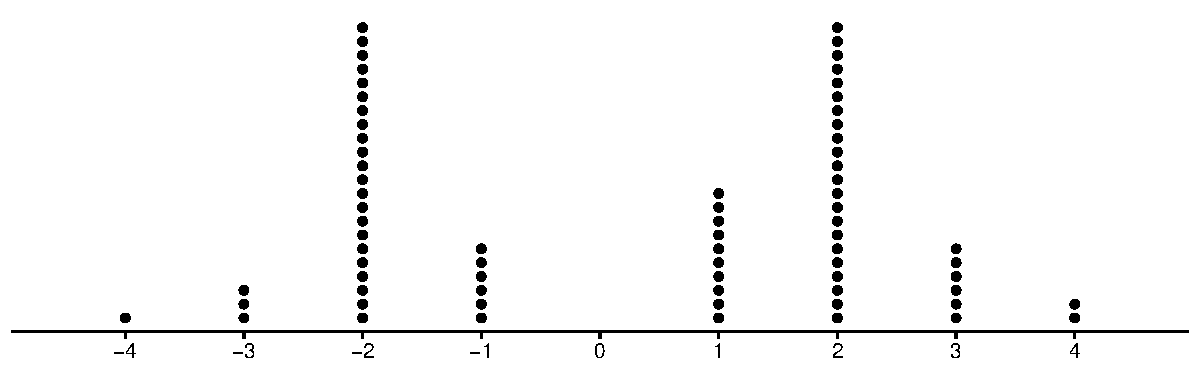
\includegraphics[width=.92\linewidth]{../figures/fhsm_2009_p88_1.pdf}
\end{center}

On the basis of this simulation, when no difference is assumed between the effects of the two types of words on memorization, a difference between medians of +4 or more occurred only two times out of $100$ trials. This result suggests that a difference between medians this large ($+4$) or larger is unlikely to occur from chance variation alone. Thus, this difference between medians would be unusual when no difference exists between the effects of the two types of words on memorization; so the use of meaningful words does seem to help when trying to memorize. 

Because this argument is based on a simulation of only $100$ trials, the statistical reasoning employed here is transitional in nature, from informal to formal. If similar results occurred after performing the simulation with a large number of trials, or if the exact probability distribution for the difference between the medians was available and indicated a similar small probability for a difference of $+4$ or more, then we could say that the difference between the medians is statistically significant (would not be expected as a result of chance variation). In this example the data provide fairly strong evidence that the use of meaningful words does help when trying to memorize.

(A more detailed illustration of students' reasoning in this problem is presented in the supporting topic book on statistics and probability.)

\noindent
\textbf{Key Elements of Mathematics}

Reasoning with Statistics and Probability---Modeling variability; Connecting statistics and probability; Interpreting designed statistical studies

\noindent
\textbf{Reasoning Habits}

Analyzing a problem---deciding whether a statistical solution is appropriate; making preliminary deductions and conjectures; seeking patterns and relationships

Implementing a strategy---making purposeful use of procedures; organizing the solution; making logical deductions

Seeking and using connections 

Reflecting on a solution---revisiting initial assumptions; justifying or validating a solution; interpreting a solution
}
{Những từ có nghĩa, Phần B}
{
\noindent
\textbf{Nhiệm vụ}

Trong Ví dụ 19, hiệu giữa hai trung vị của số từ được ghi nhớ (Có nghĩa - Vô nghĩa) là bốn từ, và việc hiệu này dương đã củng cố giả thuyết rằng học sinh có xu hướng ghi nhớ các từ có nghĩa tốt hơn so với các từ vô nghĩa. Việc phân công ngẫu nhiên được sử dụng để chia lớp thành hai nhóm với hy vọng tạo ra các nhóm tương đương. Cụ thể, phân công ngẫu nhiên có khả năng tạo ra hai nhóm tương tự nhau đối với tất cả các biến ở thời điểm bắt đầu nghiên cứu, và sự khác biệt duy nhất giữa hai nhóm ở cuối nghiên cứu là một nhóm được yêu cầu ghi nhớ các từ có nghĩa, còn nhóm kia ghi nhớ các từ vô nghĩa.

Xác suất cung cấp một cách thức để đánh giá mức độ mạnh yếu của bằng chứng thể hiện qua hiệu giữa hai trung vị. Cụ thể, vì phân công ngẫu nhiên được kỳ vọng tạo ra các nhóm tương tự nhau, nên câu hỏi đặt ra là: hiệu giữa hai trung vị quan sát được có hợp lý nếu chỉ do biến thiên ngẫu nhiên sinh ra từ việc phân công ngẫu nhiên hay không, hay hiệu này nhiều khả năng là do việc một danh sách gồm các từ có nghĩa còn danh sách kia gồm các từ vô nghĩa?

Hãy thiết kế và triển khai một mô phỏng để giải quyết câu hỏi này.

\noindent
\textbf{Trong lớp học (Lớp 12)}

Giả định rằng học sinh đã có một mức độ làm quen nhất định với phân công ngẫu nhiên như một phương pháp kiểm soát các biến gây nhiễu và tạo ra các nhóm tương đương trong một nghiên cứu thực nghiệm. Sau khi thảo luận trong lớp, học sinh luận rằng nếu hai danh sách (từ có nghĩa và từ vô nghĩa) không có ảnh hưởng gì đến khả năng ghi nhớ, thì hiệu giữa hai trung vị quan sát được chỉ là kết quả của biến thiên được kỳ vọng từ việc phân công ngẫu nhiên vào các nhóm (tức là do sự khác biệt tự nhiên giữa các học sinh). Lưu ý rằng một kiểu luận tương tự đã được sử dụng trong Ví dụ 21, khi học sinh giả định rằng quá trình lựa chọn là thực sự ngẫu nhiên.

Nếu hai danh sách khác nhau không ảnh hưởng gì đến việc ghi nhớ, thì điểm số của một học sinh sẽ không phụ thuộc vào việc em ấy ghi nhớ các từ có nghĩa hay các từ vô nghĩa. Vì thế, số từ mà một học sinh nhớ lại sẽ là như nhau bất kể em ấy được phân vào nhóm nào. Tình huống này có thể được mô phỏng bằng cách viết mỗi một trong ba mươi điểm số lên một thẻ riêng, mỗi thẻ một điểm, rồi xáo các thẻ ấy và chia ra mười lăm thẻ. Mười lăm thẻ được chia ra sẽ biểu diễn các điểm số của nhóm các từ có nghĩa; mười lăm thẻ còn lại sẽ biểu diễn các điểm số của nhóm các từ vô nghĩa. Khi đó có thể xác định trung vị của mỗi nhóm và chênh lệch giữa hai trung vị, (có nghĩa---vô nghĩa). Vì phỏng đoán ban đầu của bài toán này là người học sẽ làm tốt hơn với các từ có nghĩa, nên điều ta muốn biết là chênh lệch này xảy ra ở mức $+4$ hoặc lớn hơn với tần suất bao nhiêu. Lặp lại mô phỏng này $100$ lần cho ra phân phối lấy mẫu mô phỏng, được biểu diễn trong biểu đồ chấm dưới đây, của chênh lệch giữa hai trung vị.

\begin{center}
  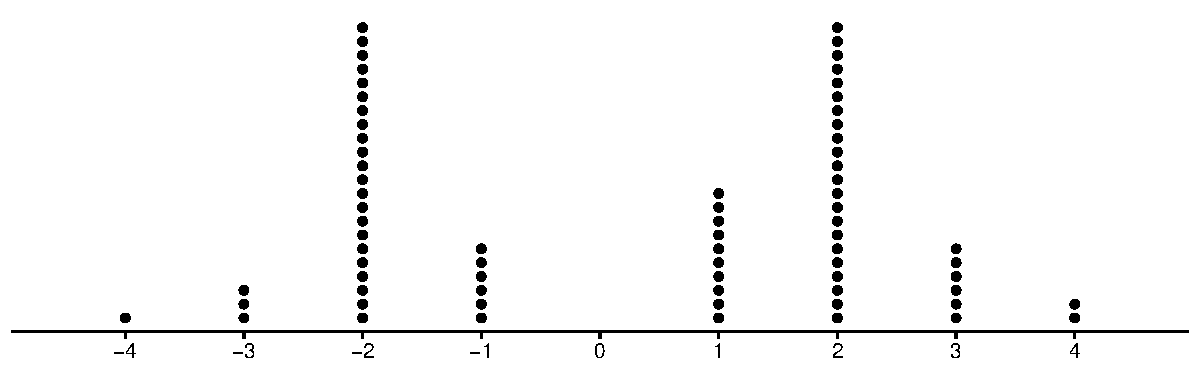
\includegraphics[width=.92\linewidth]{../figures/fhsm_2009_p88_1.pdf}
\end{center}

Dựa trên mô phỏng này, khi giả định rằng không có sự khác biệt giữa tác động của hai loại từ đối với việc ghi nhớ, thì hiệu giữa hai trung vị bằng $+4$ hoặc lớn hơn chỉ xảy ra hai lần trong $100$ lần thử. Kết quả này cho thấy một hiệu giữa hai trung vị lớn như vậy ($+4$) hoặc lớn hơn khó có khả năng xảy ra chỉ do biến thiên ngẫu nhiên. Do đó, một hiệu giữa hai trung vị như thế là bất thường khi giả định rằng hai loại từ không có tác động khác nhau đến việc ghi nhớ; vì vậy, việc sử dụng các từ có nghĩa dường như thực sự giúp ích cho quá trình ghi nhớ.

Vì biện giải này dựa trên một mô phỏng chỉ gồm $100$ lần thử, nên kiểu luận thống kê được sử dụng ở đây mang tính chuyển tiếp, từ không hình thức sang hình thức. Nếu các kết quả tương tự xuất hiện khi thực hiện mô phỏng với số lần thử lớn hơn, hoặc nếu phân bố xác suất chính xác cho hiệu giữa hai trung vị được biết đến và cũng cho thấy xác suất nhỏ đối với hiệu $+4$ hoặc lớn hơn, thì ta có thể kết luận rằng hiệu giữa hai trung vị là có ý nghĩa thống kê (không được kỳ vọng xuất hiện do biến thiên ngẫu nhiên). Trong ví dụ này, dữ liệu cung cấp bằng chứng khá mạnh mẽ cho thấy việc sử dụng các từ có nghĩa giúp cải thiện khả năng ghi nhớ.

(Một minh họa chi tiết hơn về cách học sinh luận trong bài toán này được trình bày trong tài liệu chuyên đề hỗ trợ về thống kê và xác suất.)

\noindent
\textbf{Các yếu tố then chốt của toán học}

Luận thống kê và xác suất---Mô hình hóa biến thiên; Kết nối thống kê và xác suất; Diễn giải các nghiên cứu thống kê được thiết kế

\noindent
\textbf{Các thói quen luận}

Phân tích bài toán---quyết định liệu một cách tiếp cận thống kê có phù hợp hay không; đưa ra những suy diễn và phỏng đoán sơ bộ; tìm kiếm các mẫu hình và quan hệ

Triển khai chiến lược---vận dụng có chủ đích các thủ tục; tổ chức lời giải; thực hiện những suy diễn có tính luận lý

Tìm kiếm và sử dụng các kết nối

Phản tư về lời giải---xem lại các giả định ban đầu; biện minh hoặc kiểm chứng một lời giải; diễn giải lời giải
}
{
Hiệu giữa hai trung vị bằng $+4$ tự nó chưa đủ để kết luận rằng các từ có nghĩa thực sự giúp ghi nhớ tốt hơn. Điều cần được xét không phải chỉ là độ lớn của hiệu ấy, mà là câu hỏi: nếu thật sự không có khác biệt nào giữa hai loại danh sách từ, thì một hiệu như vậy có còn là điều bình thường do cách chia nhóm ngẫu nhiên tạo ra hay không. Chính tại đây suy luận thống kê bắt đầu: một kết quả quan sát được chỉ có thể được đánh giá khi đặt nó trong quan hệ với một mô hình của biến thiên ngẫu nhiên. 

Giả định nền của ví dụ là hai loại danh sách không tạo ra khác biệt thật sự đối với khả năng ghi nhớ. Khi giữ giả định ấy, điểm số được xem là thuộc về từng học sinh, còn việc một học sinh rơi vào nhóm “có nghĩa” hay “vô nghĩa” chỉ là hệ quả của phân công ngẫu nhiên. Như vậy, câu hỏi trung tâm trở thành: nếu chỉ thay đổi cách chia ngẫu nhiên ba mươi học sinh thành hai nhóm mười lăm và mười lăm, thì hiệu giữa hai trung vị thường dao động ra sao, và một giá trị bằng $+4$ hoặc lớn hơn xuất hiện thường xuyên hay hiếm. 

Mô phỏng được đưa vào để trả lời chính câu hỏi đó. Vì chưa dễ tính trực tiếp xác suất của hiệu giữa hai trung vị ở mức phổ thông, học sinh giữ nguyên ba mươi điểm số đã có, rồi liên tục xáo trộn việc gán chúng vào hai nhóm. Mỗi lần chia lại như vậy tạo ra một “thế giới có thể xảy ra” dưới giả định không có tác động thật, từ đó cho ra một hiệu trung vị mới. Lặp lại nhiều lần sẽ tạo thành một phân bố mô phỏng của hiệu giữa hai trung vị. Phân bố ấy đóng vai trò chuẩn tham chiếu: nó cho thấy nếu không có khác biệt thật thì những hiệu nào là bình thường, những hiệu nào là hiếm.

Biểu đồ chấm vì thế không phải là hình vẽ trang trí thêm vào cho bài toán, mà là cách nhìn thấy trực tiếp biến thiên ngẫu nhiên do phân công ngẫu nhiên gây ra. Mỗi chấm là một lần mô phỏng; toàn bộ đám chấm cho biết hiệu trung vị sẽ phân bố ra sao nếu chỉ có ngẫu nhiên tác động. Khi giá trị quan sát được, ở đây là $+4$, rơi vào vùng rất ít xuất hiện của phân bố ấy, nó trở thành một kết quả khó giải thích chỉ bằng ngẫu nhiên. Việc chỉ có $2$ lần trên $100$ lần mô phỏng cho hiệu bằng $+4$ hoặc lớn hơn cho thấy kết quả quan sát được là khá hiếm dưới giả định không tác động. Bởi vậy, dữ liệu tạo ra bằng chứng khá mạnh chống lại giả định ban đầu và nghiêng về phía nhận định rằng các từ có nghĩa thực sự giúp ghi nhớ tốt hơn.

Giá trị sư phạm đặc biệt của ví dụ nằm ở chỗ nó làm sáng tỏ toàn bộ xương sống của suy luận thống kê mà không cần đi thẳng vào một công thức kiểm định hình thức: bắt đầu từ một kết quả quan sát được, đặt một giả định nền, mô hình hóa biến thiên ngẫu nhiên dưới giả định ấy, rồi so sánh kết quả quan sát với mô hình để xem nó còn hợp lí hay không. Chính cấu trúc này nối liền dữ liệu thực nghiệm ở Ví dụ 19 với mô hình xác suất và phân bố lấy mẫu ở các ví dụ trước, và làm cho ``ý nghĩa thống kê'' hiện ra như tính hiếm của một kết quả dưới một giả định xác định, chứ không phải như một nhãn gắn thêm ở cuối lời giải. 
}

\CloseGrid

% ========
%  PHẦN 3
% ========
\PartPage
{Reasoning and Sense Making in the High School Mathematics Program}
{Luận và hiểu trong chương trình toán trung học phổ thông}
{}


\OpenGrid

% ==========
%  CHƯƠNG 9
% ==========
\ParallelChapter
{Equity}
{Công bằng}
{}

\TriPara
{
\EN{
\begin{flushright}
  \emph{Mathematical reasoning and sense making must be evident in the mathematical experiences of all students.}
\end{flushright}}
}
{
\VI{
\begin{flushright}
  \emph{Luận toán học và hiểu toán học phải được thể hiện rõ trong trải nghiệm học toán của mọi học sinh.}
\end{flushright}}
}
{
\NOTE{Xác lập một lập trường xuyên suốt của chương: luận toán học và hiểu toán học không phải là đặc quyền của một nhóm học sinh có năng lực cao, cũng không phải là phần bổ sung sau khi đã học xong nội dung. Chúng phải hiện diện một cách nhận thấy được trong chính trải nghiệm học toán của mọi học sinh.}
}

\TriPara
{
\EN{In this publication, we build on the concept of equity as defined in \emph{Principles and Standards for School Mathematics} (NCTM 2000a), in which equity is described in terms of having high expectations of, and providing support for, all students. This population includes students of all races and cultures; students with low socioeconomic backgrounds; students whose first language is not English; both girls and boys; both gifted and low-achieving students; and students with learning disabilities, emotional problems, and behavioral problems. All too frequently, one or another of these groups is deemed too difficult to teach. Often, well-meaning teachers and administrators cause inequity through practices that create biases they do not intend. High schools can monitor equity by paying focused attention to phenomena that pose potential barriers to engaging every student in reasoning and sense making. These phenomena include the following:

\begin{itemize}
  \item The \emph{courses} that students take have an impact on the opportunities that they have for reasoning and sense making.
  \item \emph{Students' demographics} too often predict the opportunities students have for reasoning and sense making.
  \item \emph{Expectations, beliefs, and biases} have an impact on the mathematical learning opportunities provided for students.
\end{itemize}
}
}
{
\VI{Trong ấn phẩm này, quan niệm về công bằng được triển khai trên cơ sở cách hiểu đã được xác định trong \emph{Principles and Standards for School Mathematics} (NCTM 2000a), theo đó công bằng được mô tả qua việc đặt kỳ vọng cao đối với mọi học sinh và đồng thời cung cấp sự hỗ trợ cần thiết cho tất cả các em. Nhóm học sinh ấy bao gồm học sinh thuộc mọi chủng tộc và nền văn hóa; học sinh có hoàn cảnh kinh tế - xã hội khó khăn; học sinh mà tiếng Anh không phải là ngôn ngữ thứ nhất; cả nữ sinh lẫn nam sinh; cả học sinh có năng khiếu lẫn học sinh có thành tích thấp; cùng những học sinh gặp khó khăn trong học tập, có vấn đề về cảm xúc hoặc có vấn đề về hành vi. Quá thường xuyên, nhóm này hay nhóm khác trong số đó bị xem là quá khó để dạy. Không ít khi, chính những giáo viên và nhà quản lý vốn có thiện ý lại tạo ra sự bất công thông qua những thực hành làm nảy sinh các thiên lệch mà bản thân họ không hề chủ ý. Các trường trung học có thể theo dõi mức độ công bằng bằng cách tập trung chú ý đến những hiện tượng có thể trở thành rào cản đối với việc lôi cuốn mọi học sinh tham gia vào luận và hiểu. Những hiện tượng ấy gồm có:

\begin{itemize}
  \item Các \emph{khóa học} mà học sinh theo học tác động đến những cơ hội mà các em có được để phát triển luận và hiểu.
  \item \emph{Đặc điểm nhân khẩu học} của học sinh quá thường xuyên dự báo trước những cơ hội mà các em có được để phát triển luận và hiểu.
  \item \emph{Kỳ vọng, niềm tin và thiên lệch} tác động đến những cơ hội học toán được tạo ra cho học sinh.
\end{itemize}}
}
{
\NOTE{}
}

\ParallelSection
{Courses}
{Các khóa học}
{}

\TriPara
{
\EN{Over the past two decades, enrollment in advanced and college-preparatory mathematics courses at the high school level has increased noticeably (Planty, Provasnik, and Daniel 2007). At the same time, high schools have continued to employ some form of tracking or ability grouping (Hallinan 2004). With the tracking of students, high schools run the risk of promoting inequitable opportunities for mathematical learning for those students placed in remedial classes or in classes on “low” or “regular” tracks. For example, teacher quality varies across tracks, with more out-of-field teachers assigned to teach low-track classes (Tate and Rousseau 2002). High schools that use tracking or ability grouping can be proactive by diligently ensuring that at every level, all mathematics courses offer students opportunities for reasoning and sense making. In addition, with proper school support and access to such opportunities, students do not have to be mired in one track for their entire high school career. Successful high schools make sure that moves to different tracks are both offered and actively supported (Education Trust 2005). Moreover, we find numerous success stories of schools that have eliminated tracking with very positive results, including gains in mathematics course taking and achievement (Garrity 2004) and large numbers of minority students going on to attend college (Alvarez and Mehan 2006). An important point to note is that these schools’ success was not attributed solely to eliminating tracking but to other elements of support for students and teachers in the schools, as well.}
}
{
\VI{Trong hai thập niên qua, số học sinh trung học theo học các khóa học toán nâng cao và các khóa học toán chuẩn bị cho bậc đại học đã tăng lên rõ rệt (Planty, Provasnik, and Daniel 2007). Đồng thời, các trường trung học vẫn tiếp tục áp dụng một số hình thức phân ban hoặc phân nhóm theo năng lực (Hallinan 2004). Khi phân học sinh theo các ban như vậy, các trường trung học có nguy cơ tạo ra những cơ hội học toán không công bằng đối với những học sinh được xếp vào các lớp phụ đạo hoặc vào các lớp thuộc ban``thấp'' hay ban ``thường''. Chẳng hạn, chất lượng giáo viên khác nhau giữa các ban, trong đó những lớp ở ban thấp thường được giao cho nhiều giáo viên dạy ngoài chuyên môn hơn (Tate and Rousseau 2002). Những trường trung học sử dụng hình thức phân ban hoặc phân nhóm theo năng lực có thể chủ động ứng phó bằng cách bảo đảm một cách nghiêm túc rằng ở mọi trình độ, tất cả các khóa học toán đều đem lại cho học sinh cơ hội để phát triển luận và hiểu. Ngoài ra, nếu có sự hỗ trợ thích đáng từ phía nhà trường và có điều kiện tiếp cận những cơ hội như vậy, học sinh không nhất thiết phải bị kẹt mãi trong một ban suốt toàn bộ những năm học trung học. Những trường trung học thành công bảo đảm rằng việc chuyển sang các ban khác không chỉ được mở ra như một khả năng mà còn được hỗ trợ một cách tích cực (Education Trust 2005). Hơn nữa, nhiều câu chuyện thành công cho thấy có những trường đã xóa bỏ việc phân ban và đạt được những kết quả rất tích cực, bao gồm sự gia tăng trong việc học các khóa toán và trong thành tích học tập (Garrity 2004), cũng như việc có số lượng lớn học sinh thuộc các nhóm thiểu số tiếp tục theo học đại học (Alvarez and Mehan 2006). Một điểm quan trọng cần lưu ý là thành công của các trường này không chỉ được quy cho riêng việc xóa bỏ phân ban, mà còn gắn với những yếu tố hỗ trợ khác dành cho học sinh và giáo viên trong nhà trường.}
}
{
\NOTE{}
}

\TriPara
{
\EN{Schools with a curricular structure in which multiple levels of the same class are offered (e.g., Informal Geometry vs. Honors Geometry or Honors Integrated Mathematics vs. Integrated Mathematics) have a responsibility to engage all students in every class in reasoning and sense making, thereby ensuring that the students are learning the same major concepts regardless of the course title.}
}
{
\VI{Các trường học có cấu trúc chương trình trong đó cùng một môn học được tổ chức ở nhiều cấp độ khác nhau (ví dụ: hình học không chính quy so với hình học nâng cao, hoặc toán tích hợp nâng cao so với toán tích hợp) có trách nhiệm bảo đảm rằng mọi học sinh trong mọi lớp học đều được tham gia vào luận và hiểu. Qua đó, nhà trường bảo đảm rằng học sinh đang học cùng những khái niệm lớn cốt lõi, bất kể tên gọi của khóa học là gì.}
}
{
\NOTE{}
}

\TriPara
{
\EN{Students' unpreparedness for algebra is a current problem for high schools and often leads to schools' needing to provide some sort of remediation or additional academic support. Schools deal with this problem in various ways, such as stretching algebra over two years or placing students in a prealgebra class. These strategies can be counterproductive, especially if the result is that students are confined to the low track with limited attention to reasoning for the duration of high school and without the opportunity to catch up to their peers. High schools can support students who are underprepared for first-year algebra without limiting their future progress. For example, some high schools take early action with struggling students by offering courses in the summer before high school or as part of after-school programs (Education Trust 2005). Other schools provide first-year algebra students with general academic support in the form of teacher and peer tutoring, Saturday programs, and double course periods for some courses (Huebner, Corbett, and Phillippo 2006). In all instances, these high schools provide support early on for those students entering high school below grade level. Although programs to support underprepared students require additional resources, schools must make additional instruction to assist these students a priority. Algebra presents great opportunities for sense making and reasoning and lays a foundation for further study in mathematics. Thus, taking steps to ensure that all first-year algebra students are supported in ways that allow them to become proficient with algebraic concepts is of crucial importance.}
}
{
\VI{Việc học sinh chưa sẵn sàng cho đại số hiện là một vấn đề ở các trường trung học phổ thông và thường khiến nhà trường phải tổ chức một số hình thức phụ đạo hoặc hỗ trợ học tập bổ sung. Các trường xử lý vấn đề này theo nhiều cách khác nhau, chẳng hạn như kéo dài chương trình đại số thành hai năm hoặc xếp học sinh vào lớp tiền đại số. Tuy nhiên, những chiến lược ấy có thể phản tác dụng, nhất là khi kết quả là học sinh bị giữ lại ở luồng thấp trong suốt thời gian học trung học, ít được chú trọng đến luận, và không có cơ hội bắt kịp các bạn cùng trang lứa. Các trường trung học có thể hỗ trợ những học sinh chưa sẵn sàng cho đại số năm đầu mà không làm hạn chế sự tiến bộ sau này của các em. Chẳng hạn, một số trường can thiệp sớm đối với học sinh gặp khó khăn bằng cách mở các khóa học vào mùa hè trước khi vào trung học hoặc tổ chức các chương trình sau giờ học (Education Trust 2005). Những trường khác hỗ trợ học sinh học đại số năm đầu bằng các hình thức hỗ trợ học tập chung như giáo viên và bạn học kèm cặp, các chương trình học vào ngày thứ Bảy, hoặc tăng số tiết cho một số môn học (Huebner, Corbett, and Phillippo 2006). Trong tất cả những trường hợp ấy, các trường này đều cung cấp sự hỗ trợ từ sớm cho những học sinh bước vào trung học khi chưa đạt mức yêu cầu tương ứng. Mặc dù các chương trình hỗ trợ học sinh chưa sẵn sàng đòi hỏi thêm nguồn lực, nhà trường vẫn phải coi việc tăng cường giảng dạy để hỗ trợ những học sinh này là một ưu tiên. Đại số mở ra nhiều cơ hội cho luận và hiểu, đồng thời đặt nền móng cho việc học toán về sau. Vì vậy, việc thực hiện các biện pháp nhằm bảo đảm rằng tất cả học sinh học đại số năm đầu đều được hỗ trợ theo những cách giúp các em nắm vững các khái niệm đại số là điều hết sức quan trọng.}
}
{
\NOTE{}
}

\TriPara
{
\EN{The increasing emphasis on assessment in schools under the No Child Left Behind (NCLB) Act of 2001 (Public Law 107-110) has important consequences for opportunities for students to engage in reasoning and sense making in the classroom. In most instances, district and school policies on assessment heavily influence decisions about curriculum in the classroom. With extreme pressure for students to perform well on state assessments, teachers find themselves spending more time teaching test-taking skills and reviewing or covering those topics that are likely to be on the test. This emphasis, coupled with the fact that often high-stakes tests focus on students' ability to do procedural tasks rather assess their reasoning and sense making, equates to students' spending less time in class on developing their reasoning and sense-making abilities. This effect is even more prevalent for teachers in low-performing, high-minority schools who, under NCLB, often have even more pressure to ensure that their students succeed (Tate and Rousseau 2006). Coherence among assessment, curricula, and instruction is instrumental to addressing this issue. A discussion about the importance of coherence is included in chapter 11.}
}
{
\VI{Việc ngày càng nhấn mạnh đến đánh giá trong nhà trường theo Đạo luật No Child Left Behind (NCLB) năm 2001 (Public Law 107-110) kéo theo những hệ quả quan trọng đối với cơ hội để học sinh tham gia vào luận và hiểu trong lớp học. Trong phần lớn trường hợp, các chính sách đánh giá ở cấp học khu và nhà trường có ảnh hưởng mạnh mẽ đến những quyết định về chương trình dạy học trong lớp. Trước áp lực rất lớn buộc học sinh phải đạt kết quả tốt trong các kỳ đánh giá cấp bang, giáo viên thường phải dành nhiều thời gian hơn cho việc dạy kỹ năng làm bài kiểm tra, cũng như ôn tập hoặc dạy lướt những nội dung có khả năng xuất hiện trong đề thi. Sự nhấn mạnh này, kết hợp với thực tế là các bài kiểm tra mang tính quyết định cao thường tập trung vào khả năng thực hiện các thao tác theo quy trình của học sinh hơn là đánh giá luận và hiểu của các em, dẫn đến việc học sinh có ít thời gian hơn trên lớp để phát triển năng lực luận và hiểu. Tác động này còn rõ nét hơn đối với giáo viên ở các trường có kết quả thấp và tỉ lệ học sinh thiểu số cao; dưới khuôn khổ của NCLB, họ thường phải chịu áp lực lớn hơn nữa để bảo đảm học sinh của mình thành công (Tate and Rousseau 2006). Sự nhất quán giữa đánh giá, chương trình học và giảng dạy giữ vai trò then chốt trong việc giải quyết vấn đề này. Một phần bàn luận về tầm quan trọng của sự nhất quán ấy được trình bày trong Chương 11.}
}
{
\NOTE{}
}

\TriPara
{
\EN{To ensure that this publication's vision becomes a reality, teachers must hold high expectations for all students and find strategies to ensure that all students, at any level and in any course, can reason mathematically by engaging in challenging mathematical tasks. One such strategy is using problems that have multiple entry points so that students at different levels of mathematical experience and with different interests can all engage meaningfully in reasoning about the problem. Using problems with multiple entry points allows students to use their individual mathematical strengths in approaching the problem and gives them opportunities to make sense of the reasoning of other students.}
}
{
\VI{Để bảo đảm rằng tầm nhìn của ấn phẩm này trở thành hiện thực, giáo viên phải đặt kỳ vọng cao đối với mọi học sinh và tìm ra những cách để bảo đảm rằng tất cả học sinh, ở bất kỳ trình độ nào và trong bất kỳ khóa học nào, đều có thể luận toán học bằng cách tham gia vào những nhiệm vụ toán học có tính thách thức. Một cách như vậy là dùng những bài toán có nhiều cách bắt đầu, để học sinh với những mức độ trải nghiệm toán học khác nhau và những mối quan tâm khác nhau đều có thể tham gia một cách có ý nghĩa vào việc luận về bài toán. Việc dùng những bài toán có nhiều cách bắt đầu cho phép học sinh vận dụng những điểm mạnh toán học riêng của mình khi tiếp cận bài toán, đồng thời tạo cơ hội cho các em hiểu cách những học sinh khác luận.}
}
{
\NOTE{}
}

\TriPara
{
\EN{Several examples in section 2 of this publication describe tasks that have multiple entry points. For instance, example 7, ``Finding Balance,'' presents a problem that can be solved with or without the use of equations. If students are able to use equations flexibly, as student 1 can in the example, they can represent the described situation symbolically, solve the equation, and find the solution. However, other students who are either less confident, have had limited experience with equations, or are unable to use them flexibly might approach the problem by first drawing a picture to represent the scenario, then move toward writing an equation. Others might use a more informal reasoning approach, such as the one used by student 2, to find the answer. Exploring multiple approaches to solving a problem can forge important connections among different mathematical domains and strengthen the reasoning abilities of all learners. In example 7, student 1's solution may help student 2 consider a more formal approach, and student 2's solution may help student 1 make sense of formal equation solving. For this reason, students should be given opportunities to discuss their different approaches with one another and work toward understanding how each approach relates to the others.}
}
{
\VI{Một số ví dụ trong Phần 2 của ấn phẩm này mô tả những nhiệm vụ có nhiều điểm vào. Chẳng hạn, Ví dụ 7, ``Tìm thế cân bằng'', đưa ra một bài toán có thể giải bằng phương trình hoặc không cần dùng phương trình. Nếu học sinh có thể sử dụng phương trình một cách linh hoạt, như học sinh 1 trong ví dụ, thì các em có thể biểu diễn tình huống ấy bằng kí hiệu, giải phương trình và tìm ra đáp án. Tuy nhiên, những học sinh khác---những em kém tự tin hơn, có ít kinh nghiệm với phương trình, hoặc chưa thể dùng phương trình một cách linh hoạt---có thể bắt đầu bằng cách vẽ hình để biểu diễn tình huống, rồi từ đó chuyển dần sang việc viết phương trình. Những học sinh khác nữa có thể dùng một cách luận không chính thức hơn, như cách học sinh 2 đã dùng, để tìm ra lời giải. Việc tìm hiểu nhiều cách khác nhau để giải một bài toán có thể tạo ra những mối liên hệ quan trọng giữa các lĩnh vực toán học khác nhau và củng cố năng lực luận của mọi người học. Trong Ví dụ 7, lời giải của học sinh 1 có thể giúp học sinh 2 nghĩ tới một cách tiếp cận hình thức hơn, còn lời giải của học sinh 2 có thể giúp học sinh 1 hiểu được cách giải phương trình theo lối hình thức. Vì vậy, học sinh cần được tạo cơ hội để trao đổi với nhau về những cách tiếp cận khác nhau của mình và cùng đi tới chỗ hiểu các cách tiếp cận ấy liên hệ với nhau như thế nào.}
}
{
\NOTE{}
}

\TriPara
{
\EN{In any given high school classroom, students manifest varied levels of readiness for mathematical content, both among those who need extra support and among those who are ready to go further than the rest of the class. Often, students are deemed ``gifted'' or mathematically ``talented'' on the basis of a series of tests. However, teachers and schools should realize that students' mathematical ``talent'' is fluid (Samuels 2008) and that although a student might show great promise in geometry, for example, she or he might need extra support with algebraic content. For those students who demonstrate readiness to move beyond the core curriculum, teachers can provide opportunities to delve more deeply into the content being studied by the rest of the class. These students must have opportunities for reasoning and sense making that maximize their mathematical learning experiences. Although acceleration is definitely one component, opportunities for enrichment, advanced content, and more in-depth study can all be part of the mathematical education of these students, as well (National Association for Gifted Children 1994). For instance, in example 15, ``Circling the Points,'' students discuss the result that three noncollinear points in a plane determine a unique circle. As a next step for a student who is interested or is ready to move beyond the task posed to the rest of the class, the teacher might pose the questions ``Do four noncollinear points in the plane determine a unique circle?'' ``What are the conditions?'' ``What are some conjectures?'' This series of questions leads the student to thinking about inscribed angles, a topic that would typically not be discussed in the course until later. Thus, the student is asked to think more deeply about the original problem assigned to the class.}
}
{
\VI{Trong bất kỳ lớp học trung học phổ thông nào, học sinh đều thể hiện những mức độ sẵn sàng khác nhau đối với nội dung Toán học, cả giữa những em cần thêm hỗ trợ lẫn những em đã sẵn sàng đi xa hơn so với phần còn lại của lớp. Thông thường, học sinh được xem là ``năng khiếu'' hoặc ``có tài năng toán học'' dựa trên kết quả của một loạt bài kiểm tra. Tuy nhiên, giáo viên và nhà trường cần nhận thức rằng “tài năng” toán học của học sinh là linh hoạt (Samuels 2008): một học sinh có thể thể hiện tiềm năng nổi trội trong hình học, chẳng hạn, nhưng lại cần thêm hỗ trợ đối với nội dung đại số. Đối với những học sinh cho thấy sự sẵn sàng để vượt ra ngoài chương trình cốt lõi, giáo viên có thể tạo cơ hội để các em đi sâu hơn vào chính nội dung mà cả lớp đang học. Những học sinh này cần có các cơ hội luận và hiểu nhằm tối đa hóa trải nghiệm học tập toán học của mình. Mặc dù tăng tốc học tập chắc chắn là một thành phần quan trọng, nhưng các cơ hội làm giàu, tiếp cận nội dung nâng cao và nghiên cứu chuyên sâu hơn cũng đều có thể là những phần cấu thành của giáo dục toán học dành cho các em (National Association for Gifted Children 1994). Chẳng hạn, trong Ví dụ 15, ``Tâm ở đâu?'', học sinh thảo luận kết quả rằng ba điểm không thẳng hàng trong một mặt phẳng xác định một đường tròn duy nhất. Là bước tiếp theo dành cho một học sinh có hứng thú hoặc đã sẵn sàng đi xa hơn nhiệm vụ chung của lớp, giáo viên có thể đặt các câu hỏi: ``Bốn điểm không thẳng hàng trong mặt phẳng có xác định một đường tròn duy nhất không?'' ``Điều kiện là gì?'' ``Có thể nêu ra những phỏng đoán nào?'' Chuỗi câu hỏi này dẫn học sinh tới việc suy nghĩ về góc nội tiếp, một chủ đề thường chỉ được bàn tới ở giai đoạn sau của khóa học. Như vậy, học sinh được yêu cầu suy nghĩ sâu hơn về chính bài toán ban đầu được giao cho cả lớp.}
}
{
\NOTE{}
}

\ParallelSection
{Student Demographics and Opportunities for Learning}
{Đặc điểm nhân khẩu học của học sinh và cơ hội học tập}
{}

\TriPara
{
\EN{Discrepancies in achievement between student groups continue to raise concern for educators, families, and leaders in the United States. As reported on the mathematics portion of the 2003 National Assessment of Educational Progress (NAEP) (Lubienski and Crockett 2007), $52$ percent of Hispanic and $61$ percent of African American eighth-grade students scored below the basic level as compared with $20$ percent of white eighth-grade students. Only $7$ percent of African American students and $12$ percent of Hispanic students scored at or above the proficient level in comparison with $37$ percent of white students. An important finding of the same study was that white ($91$ percent) students were more likely to have fully credentialed teachers than African American ($80$ percent) and Hispanic ($83$ percent) students. This finding, coupled with the fact that students of teachers who majored in mathematics in college scored seven to fifteen points higher on NAEP than students of teachers who were not mathematics majors (Lubienski and Crockett 2007), indicates an important connection between discrepancies in resources and achievement.}
}
{
\VI{Những chênh lệch về thành tích giữa các nhóm học sinh tiếp tục gây quan ngại cho các nhà giáo dục, gia đình và các nhà lãnh đạo tại Hoa Kỳ. Theo báo cáo phần toán học của Kỳ đánh giá quốc gia về tiến bộ giáo dục (National Assessment of Educational Progress - NAEP) năm 2003 (Lubienski và Crockett 2007), có tới $52$ phần trăm học sinh lớp 8 người gốc Tây Ban Nha và $61$ phần trăm học sinh lớp 8 người Mỹ gốc Phi đạt điểm dưới mức cơ bản, so với $20$ phần trăm học sinh da trắng lớp 8. Chỉ $7$ phần trăm học sinh Mỹ gốc Phi và $12$ phần trăm học sinh gốc Tây Ban Nha đạt mức thành thạo trở lên, trong khi con số này ở học sinh da trắng là $37$ phần trăm. Một phát hiện quan trọng khác của cùng nghiên cứu cho thấy học sinh da trắng ($91$ phần trăm) có khả năng cao hơn được học với những giáo viên có đầy đủ chứng chỉ chuyên môn so với học sinh Mỹ gốc Phi ($80$ phần trăm) và học sinh gốc Tây Ban Nha ($83$ phần trăm). Phát hiện này, kết hợp với thực tế rằng học sinh của những giáo viên tốt nghiệp đại học chuyên ngành toán đạt điểm NAEP cao hơn từ bảy đến mười lăm điểm so với học sinh của những giáo viên không chuyên toán (Lubienski và Crockett 2007), cho thấy mối liên hệ quan trọng giữa sự chênh lệch về nguồn lực và thành tích học tập.}
}
{
\NOTE{}
}

\TriPara
{
\EN{Educators in the United States continue to grapple with economic inequity, which has a significant impact on districts' and schools' abilities to improve the opportunities to learn for the country's most underserved students (Tate and Rousseau 2007). Astounding discrepancies remain between the amount of money spent by the wealthiest districts as compared with that spent by the poorest, often high-minority, urban districts (Darling-Hammond 2004). These discrepancies exist between states as well as within states. Districts that spend more money often have smaller class sizes and more instructional resources, are able to offer a wider range of classes, and have teachers who are better paid and more experienced (Darling-Hammond 2004)}
}
{
\VI{Các nhà giáo dục tại Hoa Kỳ vẫn đang phải vật lộn với bất công về kinh tế, một yếu tố có tác động đáng kể đến khả năng của các học khu và nhà trường trong việc cải thiện cơ hội học tập cho những học sinh bị thiệt thòi nhất của quốc gia (Tate và Rousseau 2007). Những chênh lệch đáng kinh ngạc vẫn tồn tại giữa mức chi tiêu của các học khu giàu có nhất so với mức chi tiêu của các học khu nghèo nhất, những học khu thường nằm ở khu vực đô thị và có tỷ lệ học sinh thiểu số cao (Darling-Hammond 2004). Các chênh lệch này tồn tại không chỉ giữa các bang mà còn ngay trong từng bang. Những học khu chi tiêu nhiều hơn thường có sĩ số lớp học nhỏ hơn và nhiều nguồn lực giảng dạy hơn, có khả năng cung cấp phổ môn học đa dạng hơn, đồng thời có đội ngũ giáo viên được trả lương cao hơn và giàu kinh nghiệm hơn (Darling-Hammond 2004).}
}
{
\NOTE{}
}

\TriPara
{
\EN{Providing students with more opportunities to learn mathematics has serious financial consequences. For example, creating Saturday or summer programs to provide additional support to those students not ready for algebra requires additional money. Unfortunately, such programs are needed most in schools or districts that often have fewer resources. Similarly, schools that are predominantly low-income, African American, or Hispanic often contend with high teacher-turnover rates. High turnover has the unfortunate consequence that those students who are most in need of the best possible teachers are very often being taught by the least experienced teachers (Bishop and Forgasz 2006). In addition, teaching out of field is more prevalent in high-minority and lowsocioeconomic schools than in other schools, with the result that poor, minority students in the United States are often being taught by teachers who are underqualified (Education Trust 2008).}
}
{
\VI{Việc tạo thêm cơ hội để học sinh học tập toán học kéo theo những hệ quả tài chính nghiêm trọng. Chẳng hạn, việc tổ chức các chương trình học vào ngày thứ Bảy hoặc trong mùa hè nhằm cung cấp sự hỗ trợ bổ sung cho những học sinh chưa sẵn sàng học đại số đòi hỏi phải có thêm kinh phí. Đáng tiếc là những chương trình như vậy lại cần thiết nhất ở những trường hoặc học khu vốn thường có ít nguồn lực hơn. Tương tự, các trường có tỷ lệ cao học sinh thuộc diện thu nhập thấp, học sinh Mỹ gốc Phi hoặc gốc Tây Ban Nha thường phải đối mặt với tỷ lệ giáo viên nghỉ việc và luân chuyển rất cao. Hệ quả đáng buồn của tình trạng này là những học sinh cần đến những giáo viên giỏi nhất lại rất thường xuyên được dạy bởi những giáo viên ít kinh nghiệm nhất (Bishop và Forgasz 2006). Bên cạnh đó, tình trạng giáo viên dạy trái chuyên môn xảy ra phổ biến hơn ở các trường có tỷ lệ học sinh thiểu số cao và điều kiện kinh tế - xã hội thấp so với các trường khác, dẫn đến việc nhiều học sinh nghèo và thuộc nhóm thiểu số tại Hoa Kỳ thường được giảng dạy bởi những giáo viên chưa đủ năng lực chuyên môn (Education Trust 2008).}
}
{
\NOTE{}
}

\TriPara
{
\EN{The vision set forth for high school mathematics in this publication depends on teachers who have strong knowledge of mathematical content. Without this knowledge and the confidence it inspires, teachers have difficulty pushing reasoning to the forefront of the curriculum. In essence, more money, resources, and better teachers are being provided to the students who come from the wealthiest families, whereas less money, fewer resources, and less-qualified teachers are provided for the students from the poorest families (Darling-Hammond 2004). Simply providing equitable resources for all students is certainly not sufficient to ensure that each student will develop reasoning and sense making in mathematics, but it is surely necessary for real progress to be made (Bishop and Forgasz 2006). Therefore, attention must be paid to such economic disparities, including attention to the distribution of high-quality teachers, if education is to improve for all students in the United States.}
}
{
\VI{Tầm nhìn về Toán học trung học phổ thông được trình bày trong ấn phẩm này phụ thuộc vào đội ngũ giáo viên có kiến thức vững vàng về nội dung toán học. Nếu thiếu nền tảng kiến thức này, và sự tự tin mà nó mang lại, giáo viên sẽ gặp khó khăn trong việc đưa luận trở thành trọng tâm của chương trình học. Thực tế cho thấy, nhiều tiền hơn, nhiều nguồn lực hơn và những giáo viên chất lượng hơn thường được cung cấp cho học sinh đến từ các gia đình giàu có nhất, trong khi học sinh đến từ các gia đình nghèo nhất lại chỉ nhận được ít tiền hơn, ít nguồn lực hơn và những giáo viên kém đủ điều kiện hơn (Darling-Hammond 2004). Chỉ riêng việc cung cấp nguồn lực công bằng cho tất cả học sinh chắc chắn chưa đủ để bảo đảm rằng mỗi học sinh sẽ phát triển được năng lực luận và hiểu trong toán học; tuy nhiên, đó chắc chắn là điều kiện cần để có thể đạt được những tiến bộ thực chất (Bishop và Forgasz 2006). Vì vậy, nếu muốn cải thiện giáo dục cho tất cả học sinh tại Hoa Kỳ, cần phải quan tâm nghiêm túc đến những chênh lệch kinh tế này, bao gồm cả việc chú ý đến sự phân bổ đội ngũ giáo viên chất lượng cao.}
}
{
\NOTE{}
}

\TriPara
{
\EN{A positive trend is that more African American, Hispanic, and Native American students are studying more advanced mathematics than in previous decades. However, persistent gaps in course taking remain between these students and their white and Asian/Pacific Islander peers. In 2004 approximately 6 percent each of African American, Hispanic, and Native American high school students graduated having completed calculus, as compared with 33 percent of Asian/Pacific Islanders and 16 percent of white students (Planty, Provasnik, and Daniel 2007). The notion that African American, Hispanic, and Native American students are not as interested in or do not value taking advanced mathematics courses as much as their white peers is simply not true. Studies have shown that especially African American and Hispanic students “sometimes have more positive attitudes towards mathematics and higher educational aspirations” (Walker 2007, p. 48) than do their white peers, particularly in the early years of high school. Yet the disparities still exist, often tied to discrepancies in resources, which can have important consequences for students' achievement in mathematics. Hoffer, Rasinski, and Moore (1995), as cited in Tate and Rousseau (2002), found that when African American students and white students completed the same mathematics courses, they had comparable achievement gains. Tate and Rousseau go on to state, “These findings suggest that [many] of racial and SES differences in mathematics achievement in grades 9 through 12 are a product of the quality and the number of mathematics courses that African American, White, Hispanic, high- and low-SES students complete during high secondary school” (p. 276). This powerful finding makes clear the need for high schools to be diligent in supporting all students, especially those students who are often underrepresented in high-level mathematics classes, to study more advanced mathematics.}
}
{
\VI{Một xu hướng tích cực là ngày càng có nhiều học sinh Mỹ gốc Phi, gốc Tây Ban Nha và người Mỹ bản địa theo học các khóa toán nâng cao hơn so với các thập niên trước. Tuy nhiên, những khoảng cách dai dẳng về việc theo học các khóa học vẫn tồn tại giữa các nhóm học sinh này với các bạn học da trắng và gốc Á/đảo Thái Bình Dương. Năm 2004, chỉ khoảng $6$ phần trăm học sinh trung học phổ thông người Mỹ gốc Phi, gốc Tây Ban Nha và người Mỹ bản địa tốt nghiệp với việc đã hoàn thành môn giải tích, so với $33$ phần trăm học sinh gốc Á/đảo Thái Bình Dương và $16$ phần trăm học sinh da trắng (Planty, Provasnik, và Daniel 2007). Quan niệm cho rằng học sinh Mỹ gốc Phi, gốc Tây Ban Nha và người Mỹ bản địa kém quan tâm hoặc không coi trọng các khóa toán nâng cao như các bạn da trắng là hoàn toàn không đúng. Các nghiên cứu cho thấy, đặc biệt là học sinh Mỹ gốc Phi và gốc Tây Ban Nha “đôi khi có thái độ tích cực hơn đối với toán học và khát vọng giáo dục cao hơn” (Walker 2007, tr. 48) so với các bạn da trắng, nhất là trong những năm đầu trung học. Tuy vậy, các chênh lệch vẫn tồn tại, thường gắn với sự khác biệt về nguồn lực, và những khác biệt này có thể kéo theo những hệ quả quan trọng đối với thành tích toán học của học sinh. Hoffer, Rasinski, và Moore (1995), được trích dẫn trong Tate và Rousseau (2002), phát hiện rằng khi học sinh Mỹ gốc Phi và học sinh da trắng hoàn thành cùng một chương trình toán học, họ đạt được mức tăng trưởng thành tích tương đương. Tate và Rousseau tiếp tục nhận định: ``Những phát hiện này cho thấy [phần lớn] các khác biệt về chủng tộc và tình trạng kinh tế - xã hội (SES) trong thành tích toán học ở các lớp 9 đến 12 là hệ quả của chất lượng và số lượng các khóa toán học mà học sinh Mỹ gốc Phi, da trắng, gốc Tây Ban Nha, thuộc SES cao và thấp hoàn thành trong giai đoạn trung học'' (tr. 276). Phát hiện mạnh mẽ này làm rõ nhu cầu các trường trung học phải chủ động và nghiêm túc hỗ trợ tất cả học sinh, đặc biệt là những học sinh thường bị đại diện thấp trong các lớp tToán trình độ cao, được theo học các khóa toán nâng cao hơn.}
}
{
\NOTE{}
}

\TriPara
{
\EN{For more students from all racial and ethnic groups and socioeconomic levels to study more advanced mathematics, they must have the opportunity to enroll in these courses in their high school career. According to the Educational Testing Service (1999), schools having a majority of low-SES students offer fewer advanced mathematics courses than wealthier schools. This outcome, too, is closely connected with a lack of resources-most important, teachers who are qualified to teach advanced mathematics. Failure to offer advanced mathematics courses not only does a great disservice to the students but also perpetuates the shortage of people prepared to enter fields in science, technology, engineering, and mathematics.}
}
{
\VI{Để có thêm nhiều học sinh thuộc mọi nhóm chủng tộc, sắc tộc và mọi mức độ kinh tế - xã hội theo học các môn toán nâng cao, các em phải có cơ hội ghi danh vào những khóa học này trong suốt quãng thời gian học trung học phổ thông. Theo Educational Testing Service (1999), những trường có đa số học sinh thuộc nhóm kinh tế - xã hội thấp thường cung cấp ít khóa toán nâng cao hơn so với các trường giàu có hơn. Kết quả này, một lần nữa, có mối liên hệ chặt chẽ với sự thiếu hụt nguồn lực, đặc biệt là giáo viên đủ trình độ để giảng dạy toán nâng cao. Việc không cung cấp các khóa toán nâng cao không chỉ gây thiệt thòi nghiêm trọng cho học sinh mà còn góp phần kéo dài tình trạng thiếu hụt nguồn nhân lực sẵn sàng bước vào các lĩnh vực khoa học, công nghệ, kỹ thuật và toán học.}
}
{
\NOTE{}
}

\TriPara
{
\EN{Encouraging all students to take advanced mathematics courses is crucial. Walker (2007) offers suggestions that include (1) providing enrichment opportunities so that all students, but especially students from groups less represented in the mathematics pipeline, see mathematics as relevant to future careers and their lives; (2) involving families and communities; and (3) in schools that are less diverse, providing opportunities for engaging in mathematics in diverse student groups. As always, teachers play a crucial role in ensuring that once students are enrolled in advanced courses, those students are able to succeed. Teacher educators and staff developers must assist teachers in learning how to support mathematical reasoning in students who require additional support. For example, teachers can support the development of mathematical reasoning in English Language Learners (ELLs) by encouraging them to discuss their mathematical thinking on a daily basis and by providing them with various opportunities to communicate mathematically. Mathematical activity in which students are asked to reason is a vehicle for enhancing the linguistic skills of students who lack English vocabulary, thus avoiding their placement in remedial mathematics classes and preventing the delay of reasoning activities in the mathematics classroom until they have mastered basic linguistic skills (Moschkovich 2007). Instruction that centers on promoting group interaction, integrates language, uses multiple  representations, and emphasizes context is important for the success of ELLs (Bay-Williams and Herrera 2007).}
}
{
\VI{Việc khuyến khích tất cả học sinh theo học các khóa toán nâng cao là điều hết sức then chốt. Walker (2007) đưa ra một số gợi ý, bao gồm: (1) cung cấp các cơ hội làm giàu học tập để mọi học sinh, đặc biệt là những học sinh thuộc các nhóm ít được đại diện trong “đường ống” toán học, nhìn thấy Toán học có liên quan đến nghề nghiệp tương lai và cuộc sống của các em; (2) huy động sự tham gia của gia đình và cộng đồng; và (3) tại những trường học có mức độ đa dạng thấp, tạo ra các cơ hội để học sinh tham gia học toán trong các nhóm học sinh đa dạng. Như thường lệ, giáo viên đóng vai trò then chốt trong việc bảo đảm rằng khi học sinh đã ghi danh vào các khóa toán nâng cao, các em có thể học tập thành công. Các nhà đào tạo giáo viên và đội ngũ phát triển chuyên môn cần hỗ trợ giáo viên học cách nâng đỡ luận toán học của những học sinh cần thêm sự hỗ trợ. Chẳng hạn, giáo viên có thể hỗ trợ sự phát triển luận toán học của học sinh học tiếng Anh như một ngôn ngữ thứ hai (English Language Learners - ELLs) bằng cách khuyến khích các em thảo luận về tư duy toán học của mình hằng ngày và tạo ra nhiều cơ hội khác nhau để các em giao tiếp toán học. Các hoạt động toán học trong đó học sinh được yêu cầu luận chính là phương tiện để tăng cường năng lực ngôn ngữ cho những học sinh còn hạn chế vốn từ tiếng Anh, qua đó tránh việc các em bị xếp vào các lớp toán bổ trợ và ngăn chặn việc trì hoãn các hoạt động luận trong lớp toán cho đến khi các em đã thành thạo các kỹ năng ngôn ngữ cơ bản (Moschkovich 2007). Việc giảng dạy chú trọng thúc đẩy tương tác nhóm, tích hợp ngôn ngữ, sử dụng nhiều dạng biểu diễn và nhấn mạnh ngữ cảnh là những yếu tố quan trọng đối với sự thành công của học sinh ELLs (Bay-Williams và Herrera 2007).}
}
{
\NOTE{}
}

\ParallelSection
{High Expectations}
{Kỳ vọng cao}
{}

\TriPara
{
\EN{In \emph{Principles and Standards for School Mathematics} (NCTM 2000a), the Equity Principle describes the importance of teachers' holding high expectations for all students. Teachers can motivate their students to perform at high levels by having and communicating high expectations, just as they can lower students' confidence in their mathematical abilities by exhibiting low expectations. Teachers' self-awareness of personal bias about who can and cannot do mathematics is an essential part of holding high expectations for all students. All too often, teachers' and administrators' views of students' ability, motivation, behavior, and future aspirations are influenced by their beliefs associated with such student identifiers as race, gender, socioeconomic status, native language, and home life. In turn, those beliefs can have serious consequences for the opportunities that a school provides to its students. By working to become aware of subconscious attitudes, teachers and administrators can strive to overcome those notions and act purposefully against social inequalities.}
}
{
\VI{Trong \emph{Principles and Standards for School Mathematics} (NCTM 2000a), Nguyên lý Công bằng nhấn mạnh tầm quan trọng của việc giáo viên giữ kỳ vọng cao đối với tất cả học sinh. Giáo viên có thể thúc đẩy học sinh đạt thành tích cao bằng cách có và truyền đạt những kỳ vọng cao, cũng giống như họ có thể làm suy giảm sự tự tin của học sinh vào năng lực toán học của bản thân nếu thể hiện những kỳ vọng thấp. Việc giáo viên tự nhận thức về những thiên lệch cá nhân liên quan đến việc ai ``có thể'' và ai ``không thể'' học toán là một phần thiết yếu của việc duy trì kỳ vọng cao đối với mọi học sinh. Quá thường xuyên, quan điểm của giáo viên và nhà quản lý về năng lực, động cơ, hành vi và khát vọng tương lai của học sinh bị chi phối bởi những niềm tin gắn với các đặc điểm như chủng tộc, giới tính, tình trạng kinh tế - xã hội, ngôn ngữ mẹ đẻ và hoàn cảnh gia đình. Đổi lại, những niềm tin đó có thể gây ra những hệ quả nghiêm trọng đối với các cơ hội học tập mà nhà trường cung cấp cho học sinh. Thông qua việc nỗ lực nhận diện các thái độ tiềm ẩn trong tiềm thức, giáo viên và nhà quản lý có thể phấn đấu vượt qua những quan niệm đó và hành động có chủ đích nhằm chống lại các bất bình đẳng xã hội.}
}
{
\NOTE{}
}

\TriPara
{
\EN{Although holding high expectations for all students is crucial, expectations alone are not enough. By taking specific action in the classroom, teachers can truly support students in meeting those high expectations. One such action is to encourage all students to share their thinking and listen to the thinking of others. Establishing a community of learning in which a multitude of approaches and solutions are encouraged and respected is a way to effect positive change (NCTM 2008). Using tasks with multiple entry points is one way to encourage this student interaction, as all students can make a meaningful contribution to the class discussion. Subtle teacher behaviors also demonstrate the belief that all students can be successful. For example, Cousins-Cooper (2000) suggested that teachers can encourage African American students when they get stuck on a problem by asking probing questions instead of showing the students how to do the problem; such behavior is important for teachers of all students. This behavior communicates to the students and all who observe the interaction that the teacher believes that her or his students can be successful in making sense of the problem and working toward a solution. Teachers must be constantly aware of the messages they communicate to students both verbally and nonverbally.}
}
{
\VI{Mặc dù việc giữ kỳ vọng cao đối với tất cả học sinh là hết sức quan trọng, chỉ riêng kỳ vọng thôi thì chưa đủ. Thông qua những hành động cụ thể trong lớp học, giáo viên mới có thể thực sự hỗ trợ học sinh đạt tới những kỳ vọng cao đó. Một hành động như vậy là khuyến khích mọi học sinh chia sẻ cách nghĩ của mình và lắng nghe cách nghĩ của người khác. Việc xây dựng một cộng đồng học tập trong đó nhiều cách tiếp cận và lời giải khác nhau được khuyến khích và tôn trọng là một cách tạo ra sự thay đổi tích cực (NCTM 2008). Sử dụng các nhiệm vụ có nhiều điểm vào là một cách để thúc đẩy sự tương tác này, bởi mọi học sinh đều có thể đóng góp một cách có ý nghĩa cho thảo luận chung của lớp. Những hành vi tinh tế của giáo viên cũng thể hiện niềm tin rằng tất cả học sinh đều có thể thành công. Chẳng hạn, Cousins-Cooper (2000) gợi ý rằng giáo viên có thể khích lệ học sinh Mỹ gốc Phi khi các em bị mắc kẹt trong một bài toán bằng cách đặt những câu hỏi gợi mở thay vì chỉ cho các em cách làm; hành vi này cũng quan trọng đối với giáo viên dạy mọi đối tượng học sinh. Cách ứng xử như vậy truyền đạt tới học sinh, và tới tất cả những người quan sát tương tác đó, rằng giáo viên tin tưởng học sinh của mình có khả năng kiến tạo ý nghĩa cho bài toán và tiến tới lời giải. Do đó, giáo viên cần liên tục ý thức về những thông điệp mà họ truyền đạt tới học sinh, cả bằng lời nói lẫn bằng các tín hiệu phi ngôn ngữ.}
}
{
\NOTE{}
}

\TriPara
{
\EN{Creating an inclusive environment in which all students-regardless of race, gender, socioeconomic status, or perceived motivation and learning ability-are engaged in reasoning and sense-making activities communicates to students a belief that everyone is expected to be successful in mathematics. Researchers have noted a tremendous difference in success rates among highminority, low-socioeconomic student populations when a culture of high expectations and a shared goal of success for all students is adopted not just by individual teachers but by the entire school, including families and the community (Gutierrez 2000; Education Trust 2005).}
}
{
\VI{Việc tạo dựng một môi trường bao trùm, trong đó mọi học sinh, bất kể chủng tộc, giới tính, tình trạng kinh tế - xã hội hay mức độ động cơ và khả năng học tập được cảm nhận, đều tham gia vào các hoạt động luận và hiểu sẽ truyền đạt tới học sinh niềm tin rằng mọi người đều được kỳ vọng sẽ thành công trong toán học. Các nhà nghiên cứu đã ghi nhận những khác biệt rất lớn về tỷ lệ thành công ở các nhóm học sinh thiểu số và có điều kiện kinh tế - xã hội khó khăn, khi một văn hóa kỳ vọng cao và mục tiêu chung về sự thành công của tất cả học sinh được chấp nhận không chỉ bởi từng giáo viên riêng lẻ mà bởi toàn bộ nhà trường, bao gồm cả gia đình và cộng đồng (Gutierrez 2000; Education Trust 2005).}
}
{
\NOTE{}
}

\ParallelSection
{Conclusion}
{Kết luận}
{}

\TriPara
{
\EN{In general, teachers and schools across North America are working tirelessly toward the goal of providing high-quality education to every student in their classrooms. However, in the shuffle of high school life, some students are inadvertently overlooked or underserved. Moreover, the same students are frequently among those overlooked-those of color, those of low or exceptionally high achievement, and those of low socioeconomic status. Teachers, teacher leaders, and administrators, along with families and the community, must constantly reflect on how educational policy and practices may work to support or fail to support giving all students the opportunities with reasoning and sense making that they need to be successful as they exit high school. Some questions to reflect on in trying to reach this goal include these: Are the students enrolled in advanced mathematics courses at a school representative of the demographics of the school? If a school employs tracking, do students move between tracks flexibly and with the support of teachers and administrators? Are decisions on course placements based on evidence rather than subjective judgments that may unintentionally reinforce group stereotypes? In any given mathematics course, are students engaged in reasoning and sense making on a daily basis?}
}
{
\VI{Nhìn chung, giáo viên và nhà trường trên khắp Bắc Mỹ đang làm việc không mệt mỏi nhằm hướng tới mục tiêu cung cấp một nền giáo dục chất lượng cao cho mọi học sinh trong lớp học của mình. Tuy nhiên, giữa nhịp sống bận rộn của bậc trung học phổ thông, một số học sinh vẫn vô tình bị bỏ sót hoặc không được phục vụ đầy đủ. Hơn nữa, những học sinh này thường lặp đi lặp lại là cùng một nhóm, học sinh thuộc các nhóm thiểu số, học sinh có thành tích thấp hoặc rất cao, và học sinh có điều kiện kinh tế - xã hội khó khăn. Giáo viên, các nhà lãnh đạo chuyên môn, nhà quản lý, cùng với gia đình và cộng đồng, cần liên tục suy ngẫm về cách các chính sách và thực hành giáo dục có thể hỗ trợ, hoặc không hỗ trợ, việc bảo đảm cho tất cả học sinh có được những cơ hội luận và hiểu cần thiết để các em có thể thành công khi rời khỏi bậc trung học. Một số câu hỏi gợi suy ngẫm để hướng tới mục tiêu này bao gồm: Học sinh ghi danh vào các khóa toán nâng cao của nhà trường có phản ánh đúng đặc điểm nhân khẩu học của nhà trường hay không? Nếu nhà trường áp dụng phân luồng, học sinh có được di chuyển giữa các luồng một cách linh hoạt và có sự hỗ trợ của giáo viên và nhà quản lý hay không? Các quyết định xếp lớp có dựa trên bằng chứng hay dựa trên những phán đoán chủ quan có thể vô tình củng cố các khuôn mẫu nhóm? Trong mỗi khóa toán cụ thể, học sinh có được tham gia vào các hoạt động luận và hiểu hằng ngày hay không?}
}
{
\NOTE{}
}

% ===========
% CHƯƠNG 10
% ===========

\ParallelChapter
{Coherence}
{Tính nhất quán}
{}

\TriPara
{
\EN{
  \begin{flushright}
    \emph{Curriculum, instruction, and assessment form a coherent whole to support reasoning and sense making.}
  \end{flushright}
}
}
{
\VI{
  \begin{flushright}
    \emph{Chương trình học, giảng dạy và đánh giá tạo thành một chỉnh thể nhất quán nhằm hỗ trợ luận và hiểu.}
  \end{flushright}
}
}
{
\NOTE{Lời đề từ này nêu ra một nguyên tắc nền tảng của Chương 10: luận và hiểu chỉ có thể được nuôi dưỡng bền vững khi chương trình học, giảng dạy và đánh giá vận hành như một chỉnh thể nhất quán. Nếu ba thành tố này không đi cùng một hướng, thì những nỗ lực thúc đẩy luận và hiểu trong lớp học sẽ dễ bị suy yếu hoặc triệt tiêu.

\noindent
\textbf{Ba khái niệm then chốt}

\begin{itemize}
  \item \emph{Curriculum} không chỉ là danh sách các chủ đề phải dạy, mà là cách các ý tưởng toán học được lựa chọn, sắp xếp và liên kết thành một lộ trình học tập. Nó trả lời câu hỏi: học sinh sẽ được gặp những ý tưởng nào, theo thứ tự nào, và với mức độ sâu ra sao.
  \item \emph{Instruction} không chỉ là việc giáo viên trình bày kiến thức, mà là toàn bộ cách tổ chức việc học trong lớp: chọn nhiệm vụ nào, đặt câu hỏi ra sao, điều phối thảo luận thế nào, và tạo cơ hội nào để học sinh tham gia vào luận và hiểu.
  \item \emph{Assessment} không chỉ là các bài kiểm tra cho điểm, mà là mọi cách nhận biết và ghi nhận việc học của học sinh. Nó cho thấy điều gì được coi là quan trọng, đồng thời tác động ngược trở lại đến cách dạy và cách học.
\end{itemize}

\noindent
\textbf{Ý nghĩa sư phạm}

Điểm cốt lõi của lời đề từ là: không thể mong học sinh phát triển luận và hiểu nếu chương trình học, giảng dạy và đánh giá gửi đi những tín hiệu khác nhau. Chẳng hạn, nếu lớp học khuyến khích học sinh giải thích và kết nối ý tưởng, nhưng đánh giá chủ yếu chỉ đòi hỏi làm đúng theo quy trình, thì điều được củng cố sau cùng sẽ không phải là luận và hiểu. Vì vậy, tính nhất quán ở đây không phải là một phẩm chất phụ thêm, mà là điều kiện cấu trúc để luận và hiểu trở thành một phần thực sự của trải nghiệm học toán.

\noindent
\textbf{Liên hệ với mạch sách}

Nếu Chương 9 đặt trọng tâm vào câu hỏi ai có cơ hội được tham gia vào luận và hiểu, thì Chương 10 chuyển sang câu hỏi những cơ hội ấy có được hệ thống hóa và nâng đỡ một cách nhất quán hay không. Trọng tâm vì thế được chuyển từ vấn đề công bằng trong tiếp cận sang vấn đề tổ chức của chương trình, dạy học và đánh giá.}
}

\TriPara
{
\EN{To achieve the vision set forth in this publication, the components of the educational system must work together for the good of the students served by the system. Curriculum, instruction, and assessment can be designed to support students' reasoning and sense making. A coherent and cohesive mathematics program requires strong alignment of these three elements.}
}
{
\VI{Để hiện thực hóa tầm nhìn được nêu ra trong ấn phẩm này, các thành tố của hệ thống giáo dục phải phối hợp với nhau vì lợi ích của học sinh mà hệ thống phục vụ. Chương trình học, giảng dạy và đánh giá có thể được thiết kế sao cho hỗ trợ luận và hiểu của học sinh. Một chương trình toán học mạch lạc và gắn kết đòi hỏi sự ăn khớp chặt chẽ giữa ba thành tố này.}
}
{
\NOTE{}
}

\ParallelSection
{Curriculum and Instruction}
{Chương trình và giảng dạy}
{}

\TriPara
{
\EN{Increasingly, calls are being made for consistency in the high school mathematics curriculum across the United States (National Science Board 2007). Several sets of recommendations propose a list of content topics delineated by grade level, reflecting a range of goals and priorities (American Diploma Project 2004; College Board 2006, 2007; ACT 2007; Achieve 2007a, 2007b; Franklin et al. 2007). This publication calls for a different type of consistency across the curriculum---curricular emphases and instructional approaches that make reasoning and sense making foundational to the content that is taught and learned. Along with the more-detailed content recommendations outlined in \emph{Principles and Standards} (NCTM 2000a), this publication provides a critical filter in examining any curriculum arrangement to ensure that the ultimate goals of the high school mathematics program are achieved.}
}
{
\VI{Ngày càng có nhiều lời kêu gọi hướng tới tính nhất quán trong chương trình toán trung học phổ thông trên toàn Hoa Kỳ (National Science Board 2007). Nhiều bộ khuyến nghị đã đề xuất danh sách các chủ đề nội dung được phân định theo từng khối lớp, phản ánh những mục tiêu và ưu tiên khác nhau (American Diploma Project 2004; College Board 2006, 2007; ACT 2007; Achieve 2007a, 2007b; Franklin et al. 2007). Tuy nhiên, ấn phẩm này kêu gọi một kiểu nhất quán khác trong toàn bộ chương trình học---đó là những trọng tâm chương trình và cách tiếp cận giảng dạy khiến luận và hiểu trở thành nền tảng của nội dung được dạy và được học. Song song với các khuyến nghị nội dung chi tiết hơn được trình bày trong *Principles and Standards* (NCTM 2000a), ấn phẩm này cung cấp một bộ lọc mang tính phê phán để xem xét bất kỳ cách sắp xếp chương trình nào, nhằm bảo đảm rằng các mục tiêu tối hậu của chương trình Toán trung học phổ thông được hiện thực hóa.}
}
{
\NOTE{}
}

\TriPara
{
\EN{Classrooms that promote the goals of this publication prepare students to view mathematics as a connected whole across mathematical domains that consistently involves reasoning and sense making. Fostering depth of students' mathematical knowledge requires classrooms in which students are actively involved in solving problems that require them to make connections among content areas and to develop mathematical reasoning habits. The selection of mathematical tasks to use in instruction is central in promoting reasoning and sense making. Consider some of the qualities of the tasks given in the examples of this publication, including whether they---

\begin{itemize}
  \item promote sound and significant mathematical content;
  \item reflect students' understandings, interests, and experiences;
  \item support the range of ways that diverse students learn mathematics;
  \item engage students' intellect by requiring reasoning and problem solving;
  \item help students build connections; and
  \item promote communication (cf. NCTM [1991]).
\end{itemize}

Without engaging tasks, teachers' efforts to promote students' reasoning will be limited, no matter how skilled their efforts. The approach common in the United States for many years (Martin 2007), in which teachers introduce a new topic, work out several examples, and then ask their students to emulate what they have seen, will not achieve the goal. A more profitable approach may be ``teaching via problem solving'' (Schroder and Lester 1989), in which teachers use engaging tasks to help students reason about, and make sense of, new mathematical ideas.}
}
{
\VI{Những lớp học thúc đẩy các mục tiêu của ấn phẩm này chuẩn bị cho học sinh nhìn nhận toán học như một chỉnh thể liên kết xuyên suốt các lĩnh vực toán học, trong đó luận và hiểu luôn hiện diện một cách nhất quán. Việc bồi dưỡng chiều sâu hiểu biết toán học của học sinh đòi hỏi những lớp học nơi các em tham gia tích cực vào việc giải quyết những bài toán buộc các em phải tạo liên hệ giữa các mảng nội dung và phát triển các thói quen luận toán học. Việc lựa chọn các nhiệm vụ toán học dùng trong giảng dạy giữ vai trò trung tâm trong việc thúc đẩy luận và hiểu. Hãy xét một số phẩm chất của các nhiệm vụ xuất hiện trong các ví dụ của ấn phẩm này, chẳng hạn liệu chúng có---

\begin{itemize}
  \item thúc đẩy nội dung toán học vững chắc và có ý nghĩa;
  \item phản ánh sự hiểu biết, mối quan tâm và trải nghiệm của học sinh;
  \item hỗ trợ những cách học toán khác nhau của những học sinh khác nhau;
  \item huy động trí tuệ của học sinh bằng cách đòi hỏi luận và giải quyết vấn đề;
  \item giúp học sinh xây dựng các mối liên kết; và
  \item thúc đẩy giao tiếp (x. NCTM [1991]).
\end{itemize}

Nếu không có các nhiệm vụ hấp dẫn, những nỗ lực của giáo viên nhằm thúc đẩy luận của học sinh sẽ bị hạn chế, cho dù các nỗ lực đó có tinh vi đến đâu. Cách tiếp cận đã phổ biến tại Hoa Kỳ trong nhiều năm (Martin 2007)---trong đó giáo viên giới thiệu một chủ đề mới, làm mẫu một số ví dụ, rồi yêu cầu học sinh bắt chước những gì đã thấy---sẽ không đạt được mục tiêu này. Một cách tiếp cận hiệu quả hơn có thể là ``dạy học thông qua giải quyết vấn đề'' (Schroder và Lester 1989), trong đó giáo viên sử dụng các nhiệm vụ hấp dẫn để giúp học sinh luận và hiểu các ý tưởng toán học mới.}
}
{
\NOTE{}
}

\TriPara
{
\EN{As stated in the Curriculum Principle, ``a curriculum is more than a collection of activities: it must be coherent, focused on important mathematics ...'' (NCTM 2000a, p. 14). Careful attention must be given to developing sequences of tasks that help students learn important mathematics. Integrated curricula are particularly well suited to meet this goal because they are designed to emphasize connections across mathematical domains. Regardless of the way a curriculum is organized, those involved in the mathematics program must do their best to ensure that all students are being given a strong preparation in mathematics that emphasizes the curricular connections needed to support effective mathematical reasoning and sense making.}
}
{
\VI{Như đã nêu trong Nguyên lý Chương trình học, ``một chương trình học không chỉ là một tập hợp các hoạt động: nó phải mạch lạc, tập trung vào những nội dung toán học quan trọng ...'' (NCTM 2000a, tr. 14). Cần dành sự chú ý cẩn trọng cho việc xây dựng các chuỗi nhiệm vụ giúp học sinh học được những nội dung toán học cốt lõi. Các chương trình tích hợp đặc biệt phù hợp với mục tiêu này vì chúng được thiết kế để nhấn mạnh các mối liên hệ giữa các lĩnh vực toán học. Bất kể chương trình được tổ chức theo cách nào, những người tham gia vào chương trình toán học đều phải nỗ lực hết sức để bảo đảm rằng mọi học sinh đều được trang bị một nền tảng toán học vững chắc, trong đó nhấn mạnh các liên kết chương trình cần thiết nhằm hỗ trợ việc tt luận và hiểu toán học một cách hiệu quả.}
}
{
\NOTE{}
}

\TriPara
{
\EN{Merely creating an organization of worthwhile mathematical tasks within a coherent curriculum is clearly not enough. The tasks must be carried out in a classroom in which a teacher has built a classroom culture that values students' reasoning and sense making. Effective instruction requires having and communicating high expectations for all students. In such learning environments, students continually explore interesting tasks, either individually or in groups, and communicate their conjectures and conclusions to others. Pedagogical techniques and carefully designed instructional materials further ensure that the focus of instruction is on students' thinking and reasoning, and provide opportunities for all students to participate. Professional development is necessary to ensure that teachers have the tools they need to build such a classroom culture. See ``Developing Reasoning Habits in the Classroom'' in chapter 2 for additional commentary on teaching practices that may help develop reasoning and sense making.}
}
{
\VI{Chỉ riêng việc tổ chức các nhiệm vụ toán học có giá trị trong một chương trình mạch lạc rõ ràng chưa đủ. Các nhiệm vụ đó cần được triển khai trong một lớp học nơi giáo viên đã xây dựng được văn hóa lớp học coi trọng luận và hiểu của học sinh. Việc giảng dạy hiệu quả đòi hỏi giáo viên phải có và truyền đạt kỳ vọng cao đối với tất cả học sinh. Trong những môi trường học tập như vậy, học sinh liên tục khám phá các nhiệm vụ hấp dẫn, một cách cá nhân hoặc theo nhóm, và trao đổi với người khác về các phỏng đoán cũng như kết luận của mình. Các kỹ thuật sư phạm và những học liệu được thiết kế cẩn trọng giúp bảo đảm rằng trọng tâm của giảng dạy nằm ở tư duy và luận của học sinh, đồng thời tạo ra cơ hội để mọi học sinh đều có thể tham gia. Hoạt động phát triển chuyên môn là cần thiết để bảo đảm rằng giáo viên có được các công cụ cần thiết nhằm xây dựng một văn hóa lớp học như vậy. Có thể xem thêm mục ``Phát triển các thói quen luận trong lớp học'' trong Chương 2 để tham khảo thêm các bình luận về những thực hành giảng dạy có thể giúp phát triển luận và hiểu.}
}
{
\NOTE{}
}

\ParallelSection
{Vertical Alignment of Curriculum}
{Sự liên thông theo chiều dọc của chương trình học}
{}

\TriPara
{
\EN{All too often students experience discontinuities as they move from one level of mathematics to another (Smith et al. 2000), from middle school to high school and from high school to postsecondary education. The alignment of mathematical expectations related to the goals of this publication is important as students move from one school level to another. To achieve the goal of curricular coherence, an open dialogue is essential among prekindergarten through grade 8 teachers, high school mathematics teachers, mathematics teacher educators, and mathematics and statistics faculty in higher education, as well as from client disciplines, to ensure continuing support and development of students' mathematical abilities.}
}
{
\VI{Quá thường xuyên, học sinh trải nghiệm những đứt gãy khi chuyển từ cấp học toán này sang cấp học toán khác (Smith et al. 2000), từ trung học cơ sở lên trung học phổ thông và từ trung học phổ thông lên giáo dục sau trung học. Việc đồng bộ các kỳ vọng toán học gắn với các mục tiêu của ấn phẩm này là hết sức quan trọng khi học sinh di chuyển giữa các cấp học. Để đạt được mục tiêu về tính mạch lạc của chương trình, cần có đối thoại cởi mở giữa giáo viên từ mầm non đến lớp 8, giáo viên toán trung học phổ thông, các nhà đào tạo giáo viên toán, giảng viên toán và thống kê trong giáo dục đại học, cũng như các ngành học sử dụng toán, nhằm bảo đảm sự hỗ trợ và phát triển liên tục các năng lực toán học của học sinh.}
}
{
\NOTE{}
}

\TriPara
{
\EN{Schools, families, policymakers, and others need to see evidence that reasoning and sense making abilities are shared goals among all levels of mathematics teaching, including elementary school mathematics, high school mathematics, and the undergraduate curriculum. The time is right to build strong partnerships among the various constituencies, and to recognize the potential beneficial consequences resulting from a mathematics curriculum that focuses on reasoning and sense making as articulated parts of the continuum from prekindergarten through grade 16.}
}
{
\VI{Các nhà trường, gia đình, nhà hoạch định chính sách và các bên liên quan khác cần nhìn thấy những bằng chứng rõ ràng rằng luận và hiểu là những mục tiêu chung được chia sẻ ở mọi cấp độ của việc dạy và học toán, bao gồm toán tiểu học, toán trung học phổ thông và chương trình đại học bậc cử nhân. Thời điểm hiện nay là thích hợp để xây dựng những quan hệ hợp tác vững chắc giữa các nhóm liên quan khác nhau, đồng thời nhận diện những hệ quả tích cực tiềm tàng của một chương trình toán học đặt luận và hiểu làm trọng tâm như những thành phần được diễn đạt rõ ràng trong một trục liên tục từ mầm non đến lớp 16.}
}
{
\NOTE{}
}

\TriPara
{
\EN{
\noindent
\textbf{\emph{Alignment with prekindergarten through grade 8 mathematics}}

This publication takes the recommendations of Curriculum Focal Points for Prekindergarten through Grade 8 Mathematics (Curriculum Focal Points) (NCTM 2006a) as its starting point for ensuring that proper alignment occurs between the middle grades and high school. For each grade level, prekindergarten through grade 8, Curriculum Focal Points outlines Focal Point content areas and describes objectives in additional areas of “related connections.” Each chapter of Curriculum
Focal Points begins with two reminders:

\begin{itemize}
  \item The ``curriculum focal points and related connections ... are the recommended content emphases for mathematics....'' That is, the objectives outlined in the additional ``related connections'' are also required material. Otherwise, students will not receive the breadth of mathematical content required for high school, particularly in the areas of data analysis, probability, and statistics.
  \item ``It is essential that these focal points be addressed in contexts that promote problem solving, reasoning, communication, making connections, and designing and analyzing representations.'' That is, teaching skills without providing a foundation in, and without giving attention to, important mathematical processes, including reasoning and sense making, will not adequately prepare students for the kinds of thinking expected in high school mathematics.
\end{itemize}

All students entering high school should have a sound base of mathematical experiences as described in the broadest interpretation of Curriculum Focal Points. 

Taking algebra in middle grades has become increasingly popular (National Center for Educational Statistics 2009). This publication contends that whenever new content is encountered-in elementary, middle, or high school-the foundation for conceptual understanding is laid, in part, through opportunities for students to reason with and about the mathematics being studied and to connect it with their prior knowledge. Therefore, middle school courses that contain significant algebraic content must build on and foster students' reasoning and sense making-including making connections across various mathematical domains-to lay a foundation for success in later courses. For students without the content background described in Curriculum Focal Points and with insufficient experience in reasoning and sense making, taking a formal algebra course prematurely will result in missed opportunities for broadening and strengthening their understanding of fundamental mathematical concepts, including those that are foundational for later success in algebra. Taking a formal algebra course too early will be counterproductive unless students have the necessary prerequisite skills because ``exposing students to such coursework before they are ready often leads to frustration, failure, and negative attitudes toward mathematics and learning'' (NCTM 2008).}
}
{
\VI{
\noindent
\textbf{\emph{Sự liên thông với toán học từ tiền mẫu giáo đến lớp 8}}

Ấn phẩm này lấy những khuyến nghị của \emph{Curriculum Focal Points for Prekindergarten through Grade 8 Mathematics (Curriculum Focal Points)} (NCTM 2006a) làm điểm xuất phát để bảo đảm có sự liên thông thích đáng giữa bậc trung học cơ sở và trung học phổ thông. Với mỗi cấp lớp từ tiền mẫu giáo đến lớp 8, \emph{Curriculum Focal Points} nêu ra các lĩnh vực nội dung trọng tâm và mô tả các mục tiêu trong những lĩnh vực bổ sung thuộc phần ``các kết nối liên quan''. Mỗi chương của \emph{Curriculum Focal Points} đều mở đầu bằng hai lời nhắc:

\begin{itemize}
  \item ``Các trọng điểm chương trình và các kết nối liên quan ... là những trọng tâm nội dung được khuyến nghị cho môn toán....'' Nói cách khác, các mục tiêu được nêu trong phần bổ sung ``các kết nối liên quan'' cũng là những nội dung bắt buộc. Nếu không, học sinh sẽ không có được bề rộng nội dung toán học cần thiết cho trung học phổ thông, đặc biệt trong các lĩnh vực phân tích dữ liệu, xác suất và thống kê.
  \item ``Điều thiết yếu là các trọng điểm này phải được đặt trong những ngữ cảnh thúc đẩy giải quyết vấn đề, luận, giao tiếp, thiết lập các kết nối, và thiết kế cũng như phân tích các biểu diễn.'' Nói cách khác, nếu chỉ dạy kỹ năng mà không xây nền tảng cho các quá trình toán học quan trọng, cũng không chú ý đến chúng, trong đó có luận và hiểu, thì học sinh sẽ không được chuẩn bị đầy đủ cho những kiểu suy nghĩ được mong đợi trong toán học trung học phổ thông.
\end{itemize}

Mọi học sinh bước vào trung học phổ thông đều cần có một nền tảng vững chắc về trải nghiệm toán học theo cách hiểu rộng nhất của \emph{Curriculum Focal Points}.

Việc học đại số ở bậc trung học cơ sở ngày càng trở nên phổ biến (National Center for Educational Statistics 2009). Ấn phẩm này cho rằng, mỗi khi học sinh gặp một nội dung mới---ở tiểu học, trung học cơ sở hay trung học phổ thông---thì nền tảng cho sự hiểu khái niệm được hình thành, một phần, nhờ những cơ hội để các em vừa dùng toán học đang học để luận, vừa luận về chính toán học ấy, đồng thời kết nối nó với kiến thức đã có. Vì vậy, những khóa học ở bậc trung học cơ sở có nội dung đại số đáng kể phải dựa trên và đồng thời nuôi dưỡng luận và hiểu của học sinh---bao gồm cả việc thiết lập các kết nối giữa các lĩnh vực toán học khác nhau---để đặt nền tảng cho thành công trong những khóa học về sau. Đối với những học sinh chưa có nền tảng nội dung như được mô tả trong \emph{Curriculum Focal Points} và cũng chưa có đủ trải nghiệm về luận và hiểu, việc học một khóa đại số chính thức quá sớm sẽ khiến các em bỏ lỡ những cơ hội để mở rộng và củng cố sự hiểu của mình về các khái niệm toán học cơ bản, trong đó có cả những khái niệm làm nền cho thành công sau này trong đại số. Việc học một khóa đại số chính thức quá sớm sẽ phản tác dụng nếu học sinh chưa có những kỹ năng cần có từ trước, bởi ``việc cho học sinh tiếp xúc với loại khóa học như vậy trước khi các em sẵn sàng thường dẫn đến nản lòng, thất bại, và thái độ tiêu cực đối với toán học và việc học'' (NCTM 2008).}
}
{
\NOTE{}
}

\TriPara
{
\EN{
\noindent
\textbf{\emph{Alignment with postsecondary education}}

\emph{Principles and Standards} (NCTM 2000a) states, ``All students are expected to study mathematics each of the four years that they are enrolled in high school'' (p. 288), and students must experience reasoning and sense making across all four years of a high-quality high school mathematics program. This expectation is reinforced in NCTM's (2006b) Position Statement on Time: ``Evidence supports the enrollment of high school students in a mathematics course every year, continuing beyond the equivalent of a second year of algebra and a year of geometry.''

However, what courses to offer students who have taken formal algebra (and perhaps even geometry) in middle school has become increasingly problematic. If students take calculus in high school, they should take rigorous courses following the Advanced Placement guidelines (College Board 2008a) so that they are prepared to continue their study of mathematics at the collegiate level. Advanced Placement Statistics has become increasingly popular (College Board 2008b) and will meet the needs of many students going on to either mathematics-related or non-mathematics-related majors in college. Developing alternative courses that meet the needs of other students should also be considered---for example, capstone courses are being developed to help students connect what they have been learning with their future goals (cf. Charles A. Dana Center 2008). All upper-level courses should continue to promote the goals of reasoning and sense making as set forth in this publication.

The recommendations in this publication are consistent with recommendations by the Mathematics Association of America (Ganter and Barker 2004, the Committee on the Undergraduate Program in Mathematics [CUPM] 2004), and the American Mathematical Association of Two-Year Colleges (2006). These organizations propose that the entire college-level mathematics curriculum, for all students, even those who take just one course, should develop ``analytical, critical reasoning, problem-solving, and communication skills...'' (CUPM 2004, pp. 5, 13). The commonalities between recommendations for the undergraduate curriculum and those of the current publication provide opportunities to strengthen articulation between high school and postsecondary education. Furthermore, the framers of this publication believe that focusing on reasoning and sense making can move us forward on important issues, such as those involving mathematics placement examinations used by postsecondary institutions and articulation on the role of technology in high school and college mathematics.}
}
{
\VI{
\noindent
\textbf{\emph{Sự liên thông với giáo dục sau trung học}}

\emph{Principles and Standards} (NCTM 2000a) nêu rõ: ``Tất cả học sinh được kỳ vọng sẽ học toán trong cả bốn năm khi các em theo học trung học phổ thông” (tr. 288), và học sinh cần trải nghiệm luận và hiểu xuyên suốt cả bốn năm của một chương trình toán trung học phổ thông chất lượng cao. Kỳ vọng này được củng cố trong Tuyên bố lập trường về Thời lượng của NCTM (2006b): “Các bằng chứng ủng hộ việc học sinh trung học phổ thông ghi danh vào một khóa toán mỗi năm, tiếp tục vượt qua mức tương đương với hai năm đại số và một năm hình học.''

Tuy nhiên, việc nên cung cấp những khóa học nào cho các học sinh đã học đại số hình thức (và thậm chí cả hình học) ngay từ trung học cơ sở ngày càng trở nên nan giải. Nếu học sinh học giải tích ở trung học phổ thông, các em cần theo học những khóa học nghiêm ngặt theo hướng dẫn của Advanced Placement (College Board 2008a) để được chuẩn bị đầy đủ cho việc tiếp tục học toán ở bậc đại học. Advanced Placement Statistics ngày càng trở nên phổ biến (College Board 2008b) và đáp ứng nhu cầu của nhiều học sinh dự định theo học các ngành có liên quan hoặc không liên quan trực tiếp đến toán học ở bậc đại học. Việc phát triển các khóa học thay thế nhằm đáp ứng nhu cầu của những học sinh khác cũng cần được xem xét---chẳng hạn, các khóa học tổng kết đang được xây dựng để giúp học sinh kết nối những gì các em đã học với các mục tiêu tương lai (x. Charles A. Dana Center 2008). Tất cả các khóa học ở bậc trên đều cần tiếp tục thúc đẩy các mục tiêu về luận và hiểu như đã nêu trong ấn phẩm này.

Các khuyến nghị trong ấn phẩm này phù hợp với những khuyến nghị của Mathematics Association of America (Ganter và Barker 2004; Ủy ban Chương trình Toán học bậc Đại học [CUPM] 2004) và American Mathematical Association of Two-Year Colleges (2006). Các tổ chức này đề xuất rằng toàn bộ chương trình toán học bậc đại học, dành cho tất cả sinh viên, kể cả những người chỉ học một môn toán duy nhất, đều cần phát triển ``kỹ năng phân tích, luận phản biện, giải quyết vấn đề và giao tiếp...'' (CUPM 2004, tr. 5, 13). Những điểm tương đồng giữa các khuyến nghị cho chương trình đại học và các khuyến nghị của ấn phẩm hiện tại mở ra cơ hội tăng cường sự ăn khớp giữa trung học phổ thông và giáo dục sau trung học. Hơn nữa, những người biên soạn ấn phẩm này tin rằng việc tập trung vào luận và hiểu có thể giúp thúc đẩy tiến bộ trong những vấn đề quan trọng, chẳng hạn như các kỳ thi xếp lớp toán được sử dụng ở bậc sau trung học và việc thống nhất quan điểm về vai trò của công nghệ trong toán học ở trung học phổ thông và đại học.}
}
{
\NOTE{}
}

\ParallelSection
{Assessment}
{Đánh giá}
{}

\TriPara
{
\EN{What we assess should reflect what we value. Assessments that support the goals of this publication will attend to students' capabilities in mathematical reasoning and sense making and contribute to students' progress in mathematics. This endeavor is essential for at least two reasons. First, we will not be able to gauge whether we are meeting our goals if those goals are not assessed. Second, high-stakes testing that concentrates primarily on procedural skills without assessing reasoning and sense making sends a message that is contrary to the vision set forth in this publication and can adversely influence instruction and students' learning. Assessment that focuses primarily on students' ability to do algebraic manipulations, apply geometric formulas, and perform basic statistical computations will lead students to believe that reasoning and sense making are not important.}
}
{
\VI{Những gì chúng ta đánh giá phải phản ánh những gì chúng ta coi trọng. Các hình thức đánh giá hỗ trợ mục tiêu của ấn phẩm này cần chú ý đến năng lực luận và hiểu toán học của học sinh, đồng thời góp phần thúc đẩy sự tiến bộ của các em trong toán học. Nỗ lực này là thiết yếu vì ít nhất hai lý do. Thứ nhất, chúng ta sẽ không thể biết liệu mình có đạt được các mục tiêu đã đặt ra hay không nếu các mục tiêu đó không được đánh giá. Thứ hai, các kỳ kiểm tra mang tính quyết định cao nếu chủ yếu tập trung vào kỹ năng thủ tục mà không đánh giá luận và hiểu sẽ gửi đi một thông điệp trái ngược với tầm nhìn của ấn phẩm này, đồng thời có thể tác động tiêu cực đến việc giảng dạy và việc học của học sinh. Những hình thức đánh giá chủ yếu nhắm vào khả năng thao tác đại số, áp dụng công thức hình học và thực hiện các phép tính thống kê cơ bản sẽ khiến học sinh tin rằng luận và hiểu không phải là điều quan trọng.}
}
{
\NOTE{}
}

\TriPara
{
\EN{Assessing students' progress in mathematics serves two distinct roles. One essential role of assessment is to provide summative measures of students' understanding of and ability to use mathematics. All too often, high-stakes tests assess minimal standards that do not reflect the content that students need for their future success. As students, educators, and the community focus on students' success in learning lower-level content, the importance of pushing students to succeed with higher-level content may be diminished. Moreover, this publication calls for further progress in the design of many high-stakes test items to better assess students' reasoning and sense making.}
}
{
\VI{Việc đánh giá sự tiến bộ của học sinh trong toán học đảm nhiệm hai vai trò khác nhau. Một vai trò thiết yếu của đánh giá là cung cấp các thước đo tổng kết về mức độ hiểu biết của học sinh đối với toán học và khả năng vận dụng toán học của các em. Quá thường xuyên, các kỳ kiểm tra mang tính quyết định cao chỉ đánh giá các chuẩn tối thiểu, vốn không phản ánh đầy đủ những nội dung mà học sinh cần cho thành công trong tương lai. Khi học sinh, giáo viên và cộng đồng cùng tập trung vào việc học sinh đạt được thành công trong việc học các nội dung ở mức thấp, tầm quan trọng của việc thúc đẩy học sinh chinh phục các nội dung ở mức cao hơn có thể bị xem nhẹ. Hơn nữa, ấn phẩm này kêu gọi những bước tiến xa hơn trong thiết kế các câu hỏi của nhiều kỳ kiểm tra mang tính quyết định cao, nhằm đánh giá tốt hơn luận và hiểu của học sinh.}
}
{
\NOTE{}
}

\TriPara
{
\EN{The second essential component of assessment is formative assessment, which is an integral part of the learning process for the student. According to Black and Wiliam (1998), formative assessment involves providing students with learning activities and, on the basis of feedback from those activities, adjusting teaching to meet the students' needs. Various forms of formative assessment can furnish information about students' reasoning and sense making. These include teacher observations, classroom discussions, student journals, student presentations, homework, and inclass tasks, as well as tests and quizzes that ask students to explain their thinking. To ensure that their assessments reflect curricular priorities, teachers must use both summative and formative instruments for assessing students' understanding of mathematics. Example 3, “Around Pi,” illustrates the use of an in-class assignment for formative assessment. Regardless of whether a grade is assigned, the teacher might design a rubric, such as that in figure 10.1, to better understand the students' progress in understanding error and relative error.}
}
{
\VI{}
}
{
\NOTE{}
}

\TriFigure
  {../figures/fhsm_2009_p105_f1.pdf}
  {../figures/fhsm_2009_p105_f1_vi.pdf}
  {A rubric for assessing responses to example 3}
  {Một bảng tiêu chí để đánh giá các câu trả lời cho Ví dụ 3.}
  {fig:fig_10.1}

\ParallelSection
{Conclusion}
{Kết luận}
{}

\TriPara
{
\EN{Alignment of curriculum, instruction, and assessment is a starting point on the road to implementing the goals set forth in this publication within the large and complex educational system of the United States. These three components cannot be viewed in isolation. Rather, decision makers or policymakers dealing with aspects of any one of these areas must ask themselves, ``Is a coherent mathematics program being developed that takes into account all three programmatic elements?''}
}
{
\VI{Sự liên thông giữa chương trình học, giảng dạy và đánh giá là điểm khởi đầu trên con đường hiện thực hóa các mục tiêu được nêu ra trong ấn phẩm này trong hệ thống giáo dục lớn và phức tạp của Hoa Kỳ. Không thể xem ba thành tố này một cách tách rời. Trái lại, những người ra quyết định hoặc hoạch định chính sách liên quan đến bất kỳ phương diện nào của một trong ba lĩnh vực ấy đều phải tự hỏi: ``Liệu có đang xây dựng một chương trình toán học nhất quán, có tính đến cả ba thành tố của chương trình hay không?''}
}
{
\NOTE{}
}

\TriPara
{
\EN{Efforts to focus the mathematics curriculum on reasoning and sense making will require responsible efforts of, and considerable work from, all stakeholders. Support will be required through governing policy statements that clearly align with the goals set forth here. The realization of these recommendations will require considerable time and resources to provide the significant professional development required for school faculty and administrators. Many of these efforts are discussed further in the next chapter.}
}
{
\VI{Những nỗ lực nhằm tập trung chương trình học toán vào luận và hiểu sẽ đòi hỏi sự tham gia có trách nhiệm, và khối lượng công việc đáng kể, từ tất cả các bên liên quan. Sự hỗ trợ là cần thiết thông qua các chính sách quản lý được xây dựng sao cho ăn khớp rõ ràng với những mục tiêu đã được nêu ra trong ấn phẩm này. Việc hiện thực hóa các khuyến nghị này sẽ cần nhiều thời gian và nguồn lực, đặc biệt để triển khai các hoạt động phát triển chuyên môn có chiều sâu dành cho đội ngũ giáo viên và cán bộ quản lý nhà trường. Nhiều khía cạnh của những nỗ lực này sẽ được bàn luận chi tiết hơn trong chương tiếp theo.}
}
{
\NOTE{}
}

% ===========
%  CHƯƠNG 11
% ===========

\ParallelChapter
{Stakeholder Involvement}
{Sự tham gia của các bên liên quan}
{}

\TriPara
{
\EN{
  \begin{flushright}
    \emph{Everyone involved must work together to ensure that reasoning and sense making are central foci of high school mathematics programs.}
  \end{flushright}}
}
{
\EN{
  \begin{flushright}
    \emph{Tất cả những người có liên quan đều phải cùng làm việc để bảo đảm rằng luận và hiểu giữ vị trí trung tâm trong các chương trình toán học ở trung học phổ thông.}
  \end{flushright}}
}
{
\NOTE{}
}

\TriPara
{
\EN{This publication sets forth an ambitious vision for the improvement of high school mathematics by refocusing it on reasoning and sense making. This refocusing is not a minor tweaking of the system but a substantial rethinking of the high school mathematics curriculum that requires the engagement of all involved in high school mathematics. Significant effort will be needed to realign the curriculum to focus on reasoning and sense making, to provide teachers with the professional development needed to develop new understanding of the curriculum, and to ensure that all students are given the resources needed to prepare them for our rapidly changing world.}
}
{
\VI{Ấn phẩm này đưa ra một tầm nhìn đầy tham vọng nhằm cải thiện toán học trung học phổ thông bằng cách tái định hướng trọng tâm sang luận và hiểu. Sự tái định hướng này không phải là một điều chỉnh nhỏ lẻ của hệ thống, mà là một sự suy nghĩ lại mang tính căn bản về chương trình toán trung học phổ thông, đòi hỏi sự tham gia của tất cả những người có liên quan đến toán học ở bậc trung học. Những nỗ lực đáng kể sẽ cần thiết để tái căn chỉnh chương trình theo hướng tập trung vào luận và hiểu; để cung cấp cho giáo viên hoạt động phát triển chuyên môn cần thiết nhằm hình thành sự hiểu biết mới về chương trình; và để bảo đảm mọi học sinh đều được cung cấp các nguồn lực cần thiết giúp các em chuẩn bị cho một thế giới đang thay đổi nhanh chóng.}
}
{
\NOTE{}
}

\TriPara
{
\EN{The following sections outline questions that decision makers can ask themselves or others as they work with different stakeholder groups to increase their engagement in improving high school mathematics. These questions are intended to form the basis for extended reflection on what is currently happening and what needs to happen, and to spur all involved to begin moving toward the goals of this publication.}
}
{
\VI{Các mục sau đây phác thảo những câu hỏi mà những người ra quyết định có thể tự đặt ra cho bản thân hoặc cho người khác khi họ làm việc với các nhóm bên liên quan khác nhau nhằm gia tăng mức độ tham gia của các nhóm này trong việc cải thiện toán học trung học phổ thông. Những câu hỏi này được thiết kế để làm nền tảng cho sự suy ngẫm mở rộng về những gì đang diễn ra trong hiện tại và những gì cần phải diễn ra trong tương lai, đồng thời thúc đẩy tất cả các bên liên quan bắt đầu hành động theo hướng tiến tới các mục tiêu của ấn phẩm này.}
}
{
\NOTE{}
}

\ParallelSection
{Students}
{Học sinh}
{}

\TriPara
{
\EN{
  \begin{itemize}
    \item Why is the study of mathematics important for high school students?
      \begin{itemize}
        \item Do students see mathematics as a useful, interesting, and creative area of study?
        \item Do they consider an understanding of mathematics to be an important tool for their future success?
        \item Are they taking as much mathematics as possible so that they will have a firm foundation for their future career or further study?
      \end{itemize}
    \item What do reasoning and sense making mean to high school students?
      \begin{itemize}
        \item Are they actively working to make sense of the mathematics they are learning?
        \item Are they developing the reasoning that underlies mathematical procedures?
      \end{itemize}
    \item Do high school students work on their mathematics (in class and at home) thoughtfully?
      \begin{itemize}
        \item Do they look for relationships and connections, both within mathematics and with other areas of inquiry-including other subjects and cocurricular activities?
        \item Do they use mathematical procedures in a mindful way that conveys their understanding of them?
        \item Do they work at effectively communicating their mathematical reasoning to their classmates and others?
      \end{itemize}
    \item Do they exhibit a productive attitude toward mathematics and its importance in making decisions about parts of their life outside of school?
  \end{itemize}}
}
{
\EN{
  \begin{itemize}
    \item Vì sao việc học toán lại quan trọng đối với học sinh trung học phổ thông?
      \begin{itemize}
        \item Học sinh có nhìn toán học như một lĩnh vực học tập hữu ích, thú vị và sáng tạo hay không?
        \item Các em có xem sự hiểu biết về toán học là một công cụ quan trọng cho thành công của mình trong tương lai hay không?
        \item Các em có học nhiều toán nhất có thể để có một nền tảng vững chắc cho nghề nghiệp tương lai hoặc cho việc học lên tiếp hay không?
      \end{itemize}
    \item Luận và hiểu có ý nghĩa gì đối với học sinh trung học phổ thông?
      \begin{itemize}
        \item Các em có đang chủ động cố gắng hiểu toán học mà mình đang học hay không?
        \item Các em có đang phát triển lối luận làm nền cho các quy trình toán học hay không?
      \end{itemize}
    \item Học sinh trung học phổ thông có làm việc với toán học của mình một cách có suy nghĩ hay không, cả trên lớp lẫn ở nhà?
      \begin{itemize}
        \item Các em có tìm kiếm các quan hệ và mối liên hệ, cả trong nội bộ toán học lẫn giữa toán học với những lĩnh vực tìm hiểu khác---bao gồm các môn học khác và các hoạt động đồng chương trình---hay không?
        \item Các em có sử dụng các quy trình toán học một cách tỉnh táo, theo cách cho thấy các em hiểu chúng hay không?
        \item Các em có nỗ lực truyền đạt một cách hiệu quả đường luận toán học của mình tới bạn cùng lớp và những người khác hay không?
      \end{itemize}
    \item Các em có thể hiện một thái độ tích cực đối với toán học và đối với tầm quan trọng của toán học trong việc đưa ra các quyết định liên quan đến những phần đời sống ngoài nhà trường của mình hay không?
  \end{itemize}}
}
{
\NOTE{Nhóm câu hỏi này đặt học sinh vào đúng vị trí trung tâm của chương: chất lượng của dạy học toán trung học phổ thông không chỉ được đo bằng nội dung đã dạy hay điểm số đã đạt, mà còn được nhận ra qua cách học sinh nhìn toán, làm việc với toán, nói về toán, và mang toán vào đời sống của mình. Vì thế, những câu hỏi này không phải là phần phụ thêm sau cùng, mà là những câu hỏi dùng để đọc xem các mục tiêu của chương có đang thực sự hiện ra trong trải nghiệm học tập của học sinh hay không.

Một câu trả lời tích cực cho câu hỏi vì sao việc học toán quan trọng không chỉ nằm ở lời khẳng định rằng “Toán quan trọng”, mà nằm ở chỗ học sinh nhận ra toán giúp mình hiểu thế giới, giải quyết vấn đề và đưa ra quyết định; các em có thể nêu những liên hệ cụ thể giữa toán với học tập, nghề nghiệp hoặc đời sống; và các em chủ động học toán để xây một nền tảng vững chắc cho tương lai, thay vì chỉ học đủ để vượt qua kỳ thi. Ở đây, dấu hiệu cần chú ý là học sinh có xem toán như một công cụ phát triển lâu dài hay chỉ như một môn học bắt buộc.

Khi hỏi luận và hiểu có ý nghĩa gì đối với học sinh, chương muốn biết liệu các em có đang thực sự sống trong hoạt động toán học hay không. Câu trả lời tích cực là: học sinh không bằng lòng với việc ra đáp số đúng mà muốn hiểu vì sao; các em đặt câu hỏi về ý nghĩa của công thức, phương pháp và kết quả; các em có thể nói được bằng lời cách mình nghĩ khi giải toán. Nếu học sinh chỉ đồng nhất luận với việc viết nhiều bước hơn hoặc trình bày dài hơn, thì điều đang hình thành chưa phải là luận theo tinh thần của sách.

Câu hỏi về việc học sinh có làm việc với toán một cách có suy nghĩ hay không đưa trọng tâm sang chất lượng của quá trình học. Một câu trả lời tích cực thể hiện ở việc học sinh tìm kiếm các mối liên hệ giữa bài này với bài khác, giữa chủ đề này với chủ đề khác, và giữa toán với những lĩnh vực khác; các em biết chọn phương pháp thay vì làm theo máy móc; và khi gặp mâu thuẫn, các em biết xem lại, điều chỉnh, hoặc kiểm tra cách làm của mình. Dấu hiệu quan trọng ở đây không phải chỉ là học sinh làm được thủ tục, mà là các em giải thích được vì sao mình dùng thủ tục ấy.

Câu hỏi về giao tiếp cho thấy luận toán học không phải là một hoạt động khép kín trong đầu từng cá nhân. Học sinh đang phát triển tốt khi các em sẵn sàng trình bày cách nghĩ của mình, có thể diễn đạt bằng lời, bằng hình, bằng ký hiệu hoặc ví dụ, và biết lắng nghe cũng như phản hồi đường luận của bạn học. Nếu lớp học chỉ có giáo viên nói còn học sinh chép lại, thì câu trả lời cho nhóm câu hỏi này chưa thể là tích cực.

Câu hỏi cuối cùng về thái độ cũng cần được hiểu cho đúng. Một thái độ tích cực đối với toán không đồng nghĩa với việc “thích Toán”, mà là thái độ mang tính xây dựng: sẵn sàng nỗ lực khi gặp khó, không né tránh toán trong những lựa chọn học tập hay nghề nghiệp, và nhận ra giá trị của toán trong các quyết định ngoài nhà trường. Dấu hiệu đáng lo là khi học sinh tự tách mình ra khỏi những cơ hội học toán với ý nghĩ rằng toán không dành cho mình.

Vì vậy, có thể trả lời ngắn gọn cho toàn bộ nhóm câu hỏi này như sau: học sinh trung học phổ thông đang được học toán đúng tinh thần của chương khi các em thấy toán có giá trị, chủ động đi vào luận và hiểu, học với sự suy xét, biết giao tiếp đường luận của mình, và hình thành một thái độ đủ vững để tiếp tục dùng toán trong học tập, công việc và đời sống. Chính theo nghĩa ấy, danh sách câu hỏi này không chỉ là một công cụ quan sát học sinh, mà còn là một thước đo để đánh giá chất lượng thực sự của chương trình toán học trung học phổ thông.}
}

\ParallelSection
{Families}
{Gia đình}
{}

\TriPara
{
\EN{
  \begin{itemize}
    \item Why should families consider mathematics important for their high school students?
      \begin{itemize}
        \item Why is a broad preparation in mathematics important?
      \end{itemize}
    \item What is meant by reasoning and sense making?
      \begin{itemize}
        \item Will their students learn the skills they need for future success?
        \item Will their students be prepared for success in college?
      \end{itemize}
    \item Do some students possess a ``mathematics gene,'' or can all students be successful in learning to reason mathematically?
    \item What courses should families ensure that their students are taking so that their students will receive high-quality preparation in mathematics?
    \item What should families look for in their students' classroom?
      \begin{itemize}
        \item What kind of homework should their students be given?
        \item What kinds of tests should their students take?
      \end{itemize}
    \item How can families best help their students study mathematics?
      \begin{itemize}
        \item Are families encouraging their students to work for true understanding rather than just for completion of homework assignments?
        \item Are families reinforcing the importance of persistence, even in the face of frustration?
      \end{itemize}
    \item What are the most important things that families should do to support the mathematics learning of their high school student?
      \begin{itemize}
        \item Are families encouraging their students to challenge themselves academically?
        \item Are families communicating that school should be their students' top priority?
      \end{itemize}
    \item What should family members do if their child shows mathematical talent?
  \end{itemize}}
}
{
\VI{
  \begin{itemize}
    \item Vì sao các gia đình nên xem toán học là quan trọng đối với con em mình ở bậc trung học phổ thông?
      \begin{itemize}
        \item Vì sao một sự chuẩn bị toàn diện về toán học lại quan trọng?
      \end{itemize}
    \item Luận và hiểu có nghĩa là gì?
      \begin{itemize}
        \item Con em họ có học được những kỹ năng cần thiết cho thành công sau này hay không?
        \item Con em họ có được chuẩn bị để thành công ở bậc đại học hay không?
      \end{itemize}
    \item Có phải chỉ một số học sinh mới có ``gen toán học'', hay mọi học sinh đều có thể thành công trong việc học cách luận toán học?
    \item Các gia đình cần bảo đảm con em mình học những khóa học nào để các em nhận được sự chuẩn bị có chất lượng cao về toán học?
    \item Các gia đình nên chú ý điều gì trong lớp học của con em mình?
      \begin{itemize}
        \item Con em họ nên được giao loại bài tập về nhà như thế nào?
        \item Con em họ nên làm những loại bài kiểm tra nào?
      \end{itemize}
    \item Các gia đình có thể giúp con em mình học toán một cách tốt nhất như thế nào?
      \begin{itemize}
        \item Các gia đình có đang khuyến khích con em mình hướng tới sự hiểu thực sự, thay vì chỉ làm cho xong bài tập về nhà hay không?
        \item Các gia đình có đang củng cố tầm quan trọng của sự bền bỉ, ngay cả khi gặp nản lòng hay không?
      \end{itemize}
    \item Những điều quan trọng nhất mà các gia đình nên làm để hỗ trợ việc học toán của con em mình ở bậc trung học phổ thông là gì?
      \begin{itemize}
        \item Các gia đình có đang khuyến khích con em mình thử thách bản thân trong học tập hay không?
        \item Các gia đình có đang truyền đạt rằng việc học ở trường phải là ưu tiên hàng đầu của con em mình hay không?
      \end{itemize}
    \item Các thành viên trong gia đình nên làm gì nếu con mình bộc lộ năng khiếu toán học?
  \end{itemize}}
}
{
\NOTE{Nhóm câu hỏi này cho thấy việc học toán của học sinh trung học phổ thông không chỉ là việc của nhà trường. Gia đình cũng là một bên có ảnh hưởng trực tiếp đến cách học sinh nhìn toán, lựa chọn con đường học tập, và ứng xử với khó khăn khi học. Vì vậy, những câu hỏi ở đây không chỉ hỏi gia đình “nên làm gì”, mà còn hỏi gia đình đang hiểu toán học như thế nào, đang gửi đến học sinh những kỳ vọng nào, và đang nâng đỡ hay vô tình thu hẹp con đường học toán của các em.

Nếu trả lời cho câu hỏi vì sao gia đình nên xem toán học là quan trọng, thì câu trả lời không nằm ở chỗ toán là một môn thi bắt buộc, mà ở chỗ toán góp phần hình thành năng lực suy nghĩ chặt chẽ, ra quyết định, và tiếp tục học lên về sau. Một sự chuẩn bị rộng về toán học là quan trọng vì nó không chỉ phục vụ cho các ngành học chuyên biệt, mà còn giữ mở nhiều cánh cửa cho học sinh trong học tập và nghề nghiệp. Gia đình càng nhìn toán như một nền tảng lâu dài, học sinh càng có khả năng nhìn việc học toán vượt ra ngoài yêu cầu trước mắt của điểm số và thi cử.

Khi hỏi luận và hiểu có nghĩa là gì, điều quan trọng là gia đình không nên chỉ nhìn vào việc con em mình có làm đúng bài hay không. Dấu hiệu tích cực là học sinh có thể giải thích cách làm, nói được vì sao mình chọn một phương pháp, và hiểu ý nghĩa của kết quả mình tìm được. Theo nghĩa đó, việc chuẩn bị cho thành công trong tương lai hay ở bậc đại học không chỉ là học hết nội dung, mà là hình thành khả năng suy nghĩ độc lập và hiểu sâu những ý tưởng toán học đang học.

Câu hỏi về ``gen toán học'' chạm tới một niềm tin rất dễ gây hại. Một cách trả lời phù hợp hơn với tinh thần của chương là: thành công trong học toán, đặc biệt trong việc học cách luận toán học, không phải là đặc quyền của một nhóm nhỏ ``có gen''. Năng lực ấy có thể được phát triển. Vì vậy, điều gia đình cần tránh là gán nhãn quá sớm rằng con mình có hay không có khiếu toán. Khi kỳ vọng bị hạ thấp từ đầu, cơ hội học tập cũng bị thu hẹp theo. Trái lại, nếu gia đình giữ một niềm tin rằng nỗ lực, hỗ trợ đúng cách, và trải nghiệm học tập có chất lượng đều có thể làm năng lực toán học lớn lên, thì học sinh sẽ có nhiều cơ hội thành công hơn.

Khi nghĩ về việc chọn các khóa học toán, gia đình không nên chỉ hỏi môn nào dễ hơn hay ít áp lực hơn. Câu hỏi đúng hơn là: khóa học đó có giúp học sinh hiểu sâu hơn không, có duy trì việc học toán một cách liên tục qua các năm không, và có mở ra cơ hội cho việc học tiếp hay không. Một sự chuẩn bị có chất lượng cao không chỉ nằm ở việc học những môn ``cao'' về danh nghĩa, mà ở chỗ học sinh được đi qua một lộ trình đủ vững, đủ liên tục, và đủ thách thức.

Những gì gia đình nên quan sát trong lớp học, bài tập và kiểm tra cũng rất quan trọng. Một lớp học tốt không chỉ yêu cầu học sinh làm đúng, mà còn tạo điều kiện để các em giải thích, trao đổi, và suy nghĩ. Bài tập về nhà tốt không chỉ là lặp lại các bước đã thấy trên lớp, mà phải đòi hỏi học sinh suy nghĩ, kết nối, và diễn đạt. Bài kiểm tra tốt không chỉ đo khả năng làm thủ tục, mà còn tạo chỗ cho học sinh trình bày đường luận của mình. Nếu gia đình chỉ nhìn vào số lượng bài tập hay điểm số, thì sẽ rất khó thấy chất lượng thực sự của trải nghiệm học toán.

Gia đình có thể hỗ trợ việc học toán tốt nhất không phải bằng cách làm thay, mà bằng cách định hướng đúng cách học. Điều đó thể hiện ở việc khuyến khích học sinh học để hiểu, không chỉ làm cho xong; xem sai lầm như một phần tự nhiên của việc học; và nhấn mạnh giá trị của sự bền bỉ ngay cả khi gặp khó khăn. Đặc biệt, khi học sinh nản lòng, thái độ của gia đình có thể quyết định rất nhiều: hoặc giúp các em hiểu rằng khó khăn là một phần của quá trình học, hoặc củng cố niềm tin sai rằng toán là thứ mình ``không hợp''.

Vì vậy, những việc cốt lõi gia đình nên làm là giữ kỳ vọng học tập nghiêm túc, khuyến khích học sinh dám nhận những thử thách thích đáng, và truyền đạt rõ rằng việc học ở trường cần được xem là một ưu tiên. Sự hỗ trợ ở đây không có nghĩa là gây áp lực thành tích, mà là tạo nên một môi trường trong đó học sinh hiểu rằng nỗ lực học tập của mình là quan trọng và đáng được nâng đỡ.

Nếu học sinh bộc lộ năng khiếu toán học, gia đình càng cần hành động cẩn trọng. Điều nên làm là tạo điều kiện để các em được học sâu hơn, được tiếp cận những cơ hội phù hợp như câu lạc bộ, dự án, hoặc các khóa học nâng cao. Tuy nhiên, việc này không nên biến thành áp lực thành tích quá sớm. Điều cần được bảo vệ không chỉ là kết quả, mà còn là niềm vui, sự tò mò, và sự chủ động trí tuệ trong việc học toán.

Nhìn chung, mục ``Gia đình'' cho thấy cải thiện việc học toán trung học phổ thông không thể chỉ trông chờ vào lớp học. Cách gia đình hiểu toán, nói về toán, chọn đường học toán cho con em mình, và phản ứng trước thành công hay khó khăn của các em đều ảnh hưởng trực tiếp đến động lực, kỳ vọng, và sự phát triển lâu dài của học sinh. Theo nghĩa đó, gia đình không đứng bên ngoài quá trình này, mà là một phần của điều kiện làm cho luận và hiểu có thể trở thành hiện thực trong việc học toán.}
}

\ParallelSection
{Teachers}
{Giáo viên}
{}

\TriPara
{
\EN{
  \begin{itemize}
    \item Are reasoning and sense making the foci of high school mathematics teachers' instruction every day and for every topic within every course?
    \item Do teachers realize and demonstrate the importance of mathematics reasoning habits and content knowledge as life skills that will ensure their students' success in the future, not just as the prerequisite for the next mathematics course that their students may take?
      \begin{itemize}
        \item Do teachers help their students see the wide range of careers that involve mathematics-for example, finance, real estate, marketing, advertising, forensics, and even sports journalism?
        \item Do teachers emphasize the practical worth of mathematics for addressing real problems and seek contexts in which mathematics can be seen as a useful and important tool for making decisions?
      \end{itemize}
    \item Do teachers see mathematics as a coherent subject in which the reasons that results are true are as important as the results themselves?
    \item Do teachers help students make sense of the mathematics for themselves?
    \item Do teachers help students develop a productive disposition toward mathematics?
    \item Do teachers strive for balance among the areas of the high school mathematics curriculum outlined in section 2 of this publication and help students find the connections among those areas?
    \item Do teachers incorporate technology in ways that enhance students' reasoning and sense making?
    \item Do teachers use a range of assessments to monitor and promote reasoning and sense making, both in identifying students' progress and in making instructional decisions?
    \item Do teachers recognize the importance of immediately beginning to focus their content and instruction on reasoning and sense making while working with administrators and policy makers toward broadly restructuring the high school mathematics program?
    \item Do teachers believe that all students are capable of, and can benefit from a focus on, reasoning and sense making, and are they providing the necessary support for students who need extra support?
      \begin{itemize}
        \item Do teachers ensure that students at all levels have mathematics experiences that are focused on reasoning and sense making?
        \item Are teachers advocates for their students, ensuring that schools offer all students the courses that are crucial for their mathematical success?
      \end{itemize}
    \item Do teachers seek out professional development opportunities that will help them gain a better understanding of the reasoning behind mathematical concepts and ways to develop mathematical reasoning in their students?
  \end{itemize}}
}
{
\VI{
  \begin{itemize}
    \item Luận và hiểu có phải là những trọng tâm trong việc giảng dạy của giáo viên toán trung học phổ thông hằng ngày, và trong mọi chủ đề của mọi khóa học hay không?
    \item Giáo viên có nhận thức và thể hiện được tầm quan trọng của các thói quen luận toán học và tri thức nội dung như những năng lực sống giúp bảo đảm thành công tương lai cho học sinh, chứ không chỉ như điều kiện cần cho khóa học toán tiếp theo mà các em có thể theo học hay không?
      \begin{itemize}
        \item Giáo viên có giúp học sinh nhìn ra phạm vi rộng lớn của những nghề nghiệp có liên quan đến toán---chẳng hạn như tài chính, bất động sản, tiếp thị, quảng cáo, pháp y, và cả báo chí thể thao---hay không?
        \item Giáo viên có nhấn mạnh giá trị thực tiễn của toán trong việc giải quyết những vấn đề thực và tìm kiếm những ngữ cảnh trong đó toán có thể được nhìn như một công cụ hữu ích và quan trọng để đưa ra quyết định hay không?
      \end{itemize}
    \item Giáo viên có nhìn toán như một môn học nhất quán, trong đó những lý do khiến một kết quả là đúng cũng quan trọng không kém chính kết quả ấy hay không?
    \item Giáo viên có giúp học sinh tự mình hiểu toán hay không?
    \item Giáo viên có giúp học sinh hình thành một khuynh hướng tích cực đối với toán hay không?
    \item Giáo viên có cố gắng giữ sự cân đối giữa các mảng của chương trình học toán trung học phổ thông được trình bày trong Phần 2 của ấn phẩm này, đồng thời giúp học sinh tìm ra các mối liên hệ giữa những mảng ấy hay không?
    \item Giáo viên có tích hợp công nghệ theo những cách giúp tăng cường luận và hiểu của học sinh hay không?
    \item Giáo viên có sử dụng nhiều hình thức đánh giá để theo dõi và thúc đẩy luận và hiểu, cả trong việc nhận diện sự tiến bộ của học sinh lẫn trong việc đưa ra các quyết định giảng dạy hay không?
    \item Giáo viên có nhận ra tầm quan trọng của việc ngay lập tức bắt đầu định hướng nội dung và việc giảng dạy của mình vào luận và hiểu, đồng thời làm việc với các nhà quản lý và những người hoạch định chính sách để từng bước tái cấu trúc rộng rãi chương trình toán học trung học phổ thông hay không?
    \item Giáo viên có tin rằng mọi học sinh đều có khả năng tham gia và đều có thể hưởng lợi từ việc đặt trọng tâm vào luận và hiểu, đồng thời có cung cấp sự hỗ trợ cần thiết cho những học sinh cần thêm hỗ trợ hay không?
      \begin{itemize}
        \item Giáo viên có bảo đảm rằng học sinh ở mọi trình độ đều có những trải nghiệm toán học lấy luận và hiểu làm trọng tâm hay không?
        \item Giáo viên có là người bênh vực cho học sinh của mình, bảo đảm rằng nhà trường cung cấp cho mọi học sinh những khóa học có ý nghĩa quyết định đối với thành công toán học của các em hay không?
      \end{itemize}
    \item Giáo viên có chủ động tìm kiếm những cơ hội phát triển chuyên môn giúp mình hiểu rõ hơn luận đứng sau các khái niệm toán học và những cách phát triển luận toán học ở học sinh hay không?
  \end{itemize}}
}
{
\NOTE{Nhóm câu hỏi này cho thấy vai trò của giáo viên không chỉ nằm ở việc truyền đạt nội dung, mà ở chỗ biến tầm nhìn của chương thành trải nghiệm học tập diễn ra mỗi ngày trong lớp học. Nếu ở mục “Học sinh” trọng tâm là những gì có thể quan sát ở người học, và ở mục “Gia đình” là những điều kiện nâng đỡ từ bên ngoài nhà trường, thì ở đây câu hỏi đặt trực tiếp vào những quyết định sư phạm hằng ngày của giáo viên. Vì vậy, các câu hỏi này không chỉ hỏi giáo viên có đồng ý với tinh thần của chương hay không, mà hỏi tinh thần ấy có thật sự hiện ra trong cách dạy, cách chọn nhiệm vụ, cách đánh giá, cách dùng công nghệ, cách nhìn học sinh, và cách tiếp tục học nghề của chính giáo viên hay không.

Trước hết, nếu trả lời cho câu hỏi liệu luận và hiểu có thật sự là trọng tâm hằng ngày của việc giảng dạy hay không, thì dấu hiệu tích cực không nằm ở một vài tiết học đặc biệt, mà ở chỗ giáo viên thường xuyên đặt câu hỏi vì sao, yêu cầu học sinh giải thích, so sánh cách làm, và diễn đạt cách nghĩ của mình trong mọi chủ đề. Nếu luận và hiểu chỉ xuất hiện ở những “bài hay” còn phần lớn thời gian trên lớp vẫn dành cho việc làm mẫu và lặp lại, thì câu trả lời cho câu hỏi này vẫn chưa thể là tích cực.

Khi đoạn văn hỏi giáo viên có nhận ra và thể hiện được tầm quan trọng của các thói quen luận toán học và tri thức nội dung như những năng lực sống hay không, điều được nhấn mạnh là giáo viên không nên trình bày toán chỉ như chiếc cầu đi đến khóa học tiếp theo. Một câu trả lời tích cực thể hiện ở việc giáo viên giúp học sinh nhìn thấy toán có liên quan đến nhiều lĩnh vực nghề nghiệp khác nhau, nhấn mạnh vai trò của toán trong việc ra quyết định, và thường xuyên đặt toán vào những ngữ cảnh cho thấy giá trị thực tiễn của nó. Khi ấy, học sinh sẽ bớt nhìn toán như một chuỗi chướng ngại phải vượt qua, mà bắt đầu nhìn nó như một công cụ để hiểu và hành động trong thế giới.

Câu hỏi về việc giáo viên có nhìn toán như một môn học nhất quán hay không đi vào đúng tinh thần cốt lõi của FHSM. Một câu trả lời tích cực là: giáo viên coi những lý do khiến một kết quả là đúng quan trọng không kém bản thân kết quả; bài học không dừng ở kết luận, mà làm lộ ra cấu trúc, giả định, và các mối liên hệ giữa những ý tưởng toán học. Theo nghĩa đó, giúp học sinh tự mình hiểu toán không phải là để học sinh tự bơi không cần nâng đỡ, mà là tạo ra những điều kiện để các em có thời gian suy nghĩ, có cơ hội thử cách tiếp cận, và có thể đi tới sự hiểu bằng hoạt động trí tuệ của chính mình thay vì chỉ sao chép kết quả của giáo viên.

Khi nói đến khuynh hướng tích cực đối với toán, điều quan trọng là không đồng nhất điều này với việc học sinh “thích toán”. Giáo viên nuôi dưỡng một khuynh hướng tích cực khi xem sai lầm như một phần của học tập, khuyến khích thử nghiệm, và củng cố sự kiên trì ngay cả khi học sinh gặp nản lòng. Ở đây, thái độ của giáo viên đối với lỗi sai, đối với lời giải chưa hoàn chỉnh, và đối với những học sinh học chậm hơn thường nói lên nhiều hơn những khẩu hiệu được treo trong lớp.

Những câu hỏi về cân bằng nội dung và các mối liên hệ nhắc rằng giáo viên không nên để chương trình học bị phân mảnh thành những mảng rời. Một câu trả lời tích cực là giáo viên chủ động giúp học sinh nhận ra sự liên hệ giữa đại số, hình học, xác suất, thống kê và các mảng khác, thay vì dạy từng phần như những khối tách biệt. Chính ở đây, yêu cầu về luận và hiểu cũng trở nên rõ hơn: học sinh chỉ thật sự hiểu sâu khi các em nhìn ra các mối liên hệ, chứ không chỉ hoàn thành từng phần việc riêng lẻ.

Câu hỏi về công nghệ cũng cần được đọc đúng trọng tâm. Công nghệ không được xem là có giá trị chỉ vì nó làm tính nhanh hơn hay trình bày đẹp hơn. Việc tích hợp công nghệ chỉ thật sự có ý nghĩa khi nó giúp học sinh nhìn thấy cấu trúc, thử nghiệm giả thuyết, kiểm tra kết quả, khám phá sự biến đổi, hoặc so sánh các biểu diễn khác nhau. Nói cách khác, công nghệ phải được dùng như một công cụ của tư duy, chứ không chỉ như một công cụ của thao tác.

Khi bàn đến đánh giá, đoạn này đòi hỏi nhiều hơn việc kiểm tra kết quả cuối cùng. Một câu trả lời tích cực là giáo viên dùng nhiều hình thức đánh giá để vừa nhận ra sự tiến bộ của học sinh, vừa điều chỉnh dạy học, đồng thời dùng những câu hỏi buộc học sinh phải giải thích, trình bày đường luận, và phản tỉnh về cách làm của mình. Nếu đánh giá chỉ đo khả năng thực hiện thủ tục, thì dù trên lớp có nói nhiều đến luận và hiểu, tín hiệu thực sự gửi đến học sinh vẫn sẽ lệch đi.

Một điểm rất quan trọng khác là giáo viên không được chờ đến khi toàn hệ thống thay đổi rồi mới thay đổi lớp học của mình. Câu hỏi ở đây gợi một câu trả lời kép: giáo viên cần bắt đầu ngay từ nội dung và cách dạy hằng ngày của mình, nhưng đồng thời cũng cần làm việc với nhà quản lý và những người hoạch định chính sách để mở rộng tác động ấy ra cấp chương trình. Điều này cho thấy giáo viên vừa là người thực hành trong lớp, vừa là một tác nhân của cải thiện hệ thống.

Câu hỏi về niềm tin vào năng lực của mọi học sinh đi thẳng vào vấn đề công bằng. Một câu trả lời tích cực không chỉ nằm ở lời tuyên bố rằng “mọi học sinh đều học được”, mà nằm ở việc giáo viên có thật sự giữ kỳ vọng cao đi kèm hỗ trợ phù hợp hay không. Điều đó thể hiện ở chỗ học sinh ở mọi trình độ đều có cơ hội tham gia vào những trải nghiệm toán học lấy luận và hiểu làm trung tâm, và giáo viên có sẵn sàng đứng ra bảo vệ quyền được học những khóa học quan trọng của học sinh hay không. Nếu một số nhóm học sinh bị mặc nhiên xem là không phù hợp với trải nghiệm toán học có chiều sâu, thì câu trả lời cho nhóm câu hỏi này phải là chưa.

Cuối cùng, câu hỏi về phát triển chuyên môn liên tục nhắc rằng giáo viên không thể nuôi dưỡng luận ở học sinh nếu chính mình chỉ nắm kỹ thuật bề mặt. Một câu trả lời tích cực là giáo viên chủ động tìm kiếm những cơ hội học nghề giúp mình hiểu sâu hơn vì sao các khái niệm toán học là đúng, đồng thời học cách thiết kế và dẫn dắt những tình huống trong đó học sinh có thể phát triển luận. Theo nghĩa đó, phát triển chuyên môn không chỉ là học thêm cách trình bày bài giảng, mà là đào sâu chính sự hiểu toán và sự hiểu sư phạm của người dạy.

Nhìn chung, mục ``Giáo viên'' cho thấy chất lượng của chương trình toán trung học phổ thông có thể được đọc ra từ những quyết định nhỏ nhưng lặp lại mỗi ngày trong lớp học. Khi giáo viên giữ luận và hiểu làm trọng tâm thường trực, xem toán như một lĩnh vực có ý nghĩa, tin vào năng lực của mọi học sinh, dùng công nghệ và đánh giá như công cụ nâng đỡ tư duy, và tiếp tục phát triển chính mình như một người dạy toán, thì tầm nhìn của chương mới có cơ hội trở thành hiện thực.}
}

\ParallelSection
{Administrators}
{Cán bộ quản lý}
{}

\TriPara
{
\EN{
  \begin{itemize}
    \item Do school districts, schools, departments, and teachers ensure that students receive a high quality high school mathematics curriculum that promotes reasoning and sense making?
    \item Do school districts support teachers through long-term professional development that includes reflection on their practice and their work to improve it?
      \begin{itemize}
        \item Do professional development activities help teachers experience mathematics as reasoning and sense making for themselves?
        \item Are teachers given time to collaborate during the school day to improve mathematics instruction-with colleagues teaching at the same level to develop tasks that promote reasoning and sense making and with those teaching at higher and lower levels to ensure that reasoning and sense making are being developed across the grades?
        \item Do teachers collaboratively analyze students' work and improve the level of forma  tive feedback for students on reasoning and sense making?
        \item Is mentoring provided for novice teachers as they work to develop students' reasoning and sense-making skills?
      \end{itemize}
    \item Do schools and school districts work with universities, including mathematicians, statisticians, and mathematics teacher educators, to develop effective programs and courses that address teachers' needs?
    \item Do administrators' classroom observations of mathematics teachers focus on reasoning and sense making and provide useful formative feedback?
    \item Are support systems in place to provide high school students with the needed assistance to attain high expectations in mathematics?
      \begin{itemize}
        \item Does the school district's counseling infrastructure promote perseverance in taking higher-level mathematics, thereby supporting the goal of increasing students' mathematical reasoning and sense making?
      \end{itemize}
  \end{itemize}}
}
{
\VI{
  \begin{itemize}
    \item Các học khu, nhà trường, tổ chuyên môn và giáo viên có bảo đảm rằng học sinh được học một chương trình toán trung học phổ thông có chất lượng cao, thúc đẩy luận và hiểu hay không?
    \item Các học khu có hỗ trợ giáo viên thông qua hoạt động bồi dưỡng chuyên môn dài hạn, trong đó có việc suy ngẫm về thực hành của mình và nỗ lực cải thiện thực hành ấy hay không?
      \begin{itemize}
        \item Các hoạt động bồi dưỡng chuyên môn có giúp giáo viên tự mình trải nghiệm toán học như một hoạt động của luận và hiểu hay không?
        \item Giáo viên có được dành thời gian để cộng tác với nhau trong ngày làm việc ở trường nhằm cải thiện việc dạy toán---với những đồng nghiệp dạy cùng cấp để cùng phát triển các nhiệm vụ thúc đẩy luận và hiểu, và với những người dạy ở các cấp cao hơn hoặc thấp hơn để bảo đảm rằng luận và hiểu đang được phát triển xuyên suốt các cấp lớp---hay không?
        \item Giáo viên có cùng nhau phân tích bài làm của học sinh và nâng cao chất lượng phản hồi thường xuyên dành cho học sinh về luận và hiểu hay không?
        \item Giáo viên mới vào nghề có được cố vấn khi họ nỗ lực phát triển các năng lực luận và hiểu cho học sinh hay không?
      \end{itemize}
    \item Nhà trường và các học khu có phối hợp với các trường đại học---bao gồm các nhà toán học, nhà thống kê và những người đào tạo giáo viên toán---để xây dựng những chương trình và khóa học hiệu quả, đáp ứng nhu cầu của giáo viên hay không?
    \item Việc dự giờ giáo viên toán của các nhà quản lý có tập trung vào luận và hiểu, đồng thời cung cấp những phản hồi thường xuyên hữu ích hay không?
    \item Có những hệ thống hỗ trợ cần thiết để giúp học sinh trung học phổ thông đạt tới những kỳ vọng cao trong toán học hay không?
      \begin{itemize}
        \item Hệ thống tư vấn của học khu có khuyến khích học sinh kiên trì theo học các khóa toán ở trình độ cao hơn, qua đó hỗ trợ mục tiêu tăng cường luận và hiểu của các em hay không?
      \end{itemize}
  \end{itemize}}
}
{
\NOTE{Nhóm câu hỏi này cho thấy việc phát triển luận và hiểu trong toán học trung học phổ thông không thể chỉ được đặt lên vai giáo viên riêng lẻ. Nó còn phụ thuộc vào những quyết định của học khu, nhà trường, tổ chuyên môn và cán bộ quản lý về chương trình học, bồi dưỡng chuyên môn, thời gian hợp tác, cơ chế hỗ trợ học sinh, cách dự giờ, và cách kết nối với các cơ sở đào tạo giáo viên. Vì vậy, các câu hỏi ở đây thực chất đang hỏi liệu hệ thống quản lý có đang tạo điều kiện để luận và hiểu trở thành thực tế trong lớp học, hay đang vô tình làm suy yếu mục tiêu ấy.

Nếu trả lời cho câu hỏi liệu học sinh có đang được học một chương trình toán trung học phổ thông có chất lượng cao hay không, thì dấu hiệu tích cực không chỉ nằm ở việc chương trình có nhiều nội dung hay có tỉ lệ đỗ cao, mà ở chỗ các quyết định về phân ban, chọn sách, xây dựng lộ trình học và đánh giá đều nhất quán với mục tiêu phát triển luận và hiểu. Một chương trình chỉ nhắm đến việc tối ưu kết quả thi cử trước mắt mà không tạo ra chiều sâu trong trải nghiệm học toán thì chưa thể được xem là có chất lượng cao theo tinh thần của chương.

Khi đoạn văn hỏi về bồi dưỡng chuyên môn dài hạn, điều được nhấn mạnh là sự thay đổi bền vững trong dạy học không thể đến từ vài buổi tập huấn ngắn. Một câu trả lời tích cực là học khu và nhà trường đầu tư vào những quá trình bồi dưỡng có tính liên tục, trong đó giáo viên có cơ hội suy ngẫm về thực hành của mình, thử nghiệm cách làm mới, rồi quay lại xem xét và cải thiện. Quan trọng hơn, các hoạt động bồi dưỡng ấy cần giúp giáo viên tự mình trải nghiệm toán như một hoạt động của luận và hiểu, chứ không chỉ học thêm cách triển khai bài dạy. Nếu giáo viên chưa từng được đặt vào vị trí người học phải suy nghĩ, giải thích và kết nối, thì rất khó để họ tạo ra trải nghiệm ấy cho học sinh.

Câu hỏi về thời gian hợp tác trong ngày làm việc cho thấy việc phát triển luận và hiểu không phải là trách nhiệm cá nhân của từng giáo viên đứng lớp, mà là một mục tiêu tập thể. Một câu trả lời tích cực là giáo viên được bố trí thời gian để làm việc cùng nhau, vừa theo chiều ngang với những người dạy cùng cấp để xây dựng nhiệm vụ và chia sẻ kinh nghiệm, vừa theo chiều dọc với những người dạy ở các cấp lớp khác nhau để bảo đảm rằng luận và hiểu được nuôi dưỡng liên tục qua các năm học. Khi giáo viên cùng nhau phân tích bài làm của học sinh và nâng cao chất lượng phản hồi thường xuyên, họ không chỉ cải thiện việc dạy từng bài riêng lẻ, mà còn dần hình thành một hiểu biết chung về những gì cần được xem là tiến bộ trong luận và hiểu.

Câu hỏi về mentoring cho giáo viên mới cũng rất quan trọng. Ở đây, mentoring không chỉ là hỗ trợ những kỹ năng quản lý lớp học hay xử lý công việc hằng ngày, mà còn là cách truyền một văn hóa sư phạm trong đó luận và hiểu được coi là trọng tâm thật sự của việc dạy toán. Nếu giáo viên mới chỉ được hướng dẫn cách giữ nề nếp và chạy kịp tiến độ, mà không được nâng đỡ để xây dựng những lớp học có chiều sâu về toán, thì mục tiêu của chương khó có thể bền vững.

Khi nói đến sự phối hợp với các trường đại học, đoạn này nhấn mạnh rằng nhà trường phổ thông không nên vận hành tách rời khỏi cộng đồng học thuật rộng hơn. Một câu trả lời tích cực là học khu và nhà trường chủ động làm việc với các nhà toán học, nhà thống kê và những người đào tạo giáo viên để xây dựng những chương trình và khóa học thực sự đáp ứng nhu cầu của giáo viên. Sự phối hợp ấy giúp bảo đảm tính học thuật, tính cập nhật, và sự gắn kết giữa toán học ở phổ thông với những kỳ vọng của bậc học cao hơn.

Câu hỏi về việc dự giờ của cán bộ quản lý cũng làm lộ rõ một vấn đề then chốt: nhà quản lý sẽ gửi tín hiệu gì cho giáo viên về điều được xem là quan trọng. Nếu việc dự giờ chỉ chú ý đến trật tự lớp học, tiến độ nội dung, hay hình thức trình bày, thì thông điệp gửi tới giáo viên sẽ dễ lệch khỏi trọng tâm của chương. Một câu trả lời tích cực là việc quan sát lớp học và phản hồi của cán bộ quản lý thực sự tập trung vào luận và hiểu, đồng thời cung cấp những góp ý thường xuyên có ích để giáo viên tiếp tục điều chỉnh thực hành của mình.

Nhóm câu hỏi cuối về hệ thống hỗ trợ học sinh đưa trọng tâm trở lại vấn đề công bằng trong cơ hội học toán. Một câu trả lời tích cực là nhà trường và học khu có những cấu trúc hỗ trợ đủ mạnh để giúp học sinh đạt tới những kỳ vọng cao, thay vì hạ thấp kỳ vọng khi các em gặp khó khăn. Điều này bao gồm hỗ trợ học tập, tư vấn chọn môn, và đặc biệt là một hạ tầng tư vấn khuyến khích học sinh kiên trì theo học các khóa toán ở trình độ cao hơn. Nếu hệ thống tư vấn vô tình dẫn học sinh tránh những môn học quan trọng vì sợ khó hoặc sợ thất bại, thì chính hệ thống ấy đang thu hẹp cơ hội phát triển luận và hiểu của học sinh.

Nhìn chung, mục “Cán bộ quản lý” cho thấy chất lượng của chương trình toán trung học phổ thông không chỉ được quyết định ở cấp lớp học, mà còn được hình thành bởi các quyết định tổ chức, phân bổ thời gian, nguồn lực, và cơ chế hỗ trợ của hệ thống quản lý. Khi học khu, nhà trường và cán bộ quản lý xây được những điều kiện để giáo viên cộng tác, được bồi dưỡng lâu dài, được phản hồi đúng trọng tâm, và để học sinh được hỗ trợ theo đuổi những trải nghiệm toán học có chiều sâu, thì luận và hiểu mới có cơ hội trở thành trọng tâm thực sự của chương trình toán trung học phổ thông.}
}

\ParallelSection
{Policymakers}
{Nhà hoạch định chính sách}
{}

\TriPara
{
\EN{
  \begin{itemize}
    \item Why is mathematics important for high school students?
    \item Why is high school mathematics education important to the economic competitiveness of the United States in the global marketplace?
    \item What is meant by reasoning and sense making in mathematics, and why should these outcomes be crucial foci in high school?
    \item Are reasoning and sense making inextricably integrated with content topics in state and district frameworks that guide curricular decisions?
    \item Do state and local assessment policies emphasize the need for, and importance of, items that examine students' ability to reason and make sense of mathematical situations?
    \item How can policymakers help ensure that all students have access to a rich mathematics curriculum based on reasoning and sense making?
    \item Are adequate resources allocated to assist schools and districts in efforts to effectively implement a curriculum based on reasoning and sense making?
  \end{itemize}}
}
{
\EN{
  \begin{itemize}
    \item Vì sao toán học lại quan trọng đối với học sinh trung học phổ thông?
    \item Vì sao giáo dục toán học trung học phổ thông lại quan trọng đối với năng lực cạnh tranh kinh tế của Hoa Kỳ trên thị trường toàn cầu?
    \item Luận và hiểu trong toán học có nghĩa là gì, và vì sao những kết quả ấy phải là những trọng tâm cốt yếu ở bậc trung học phổ thông?
    \item Luận và hiểu có được gắn kết chặt chẽ, không thể tách rời, với các chủ đề nội dung trong các khung chương trình của bang và học khu, vốn định hướng cho các quyết định về chương trình học, hay không?
    \item Các chính sách đánh giá ở cấp bang và địa phương có nhấn mạnh nhu cầu và tầm quan trọng của những câu hỏi nhằm xem xét khả năng luận và hiểu các tình huống toán học của học sinh hay không?
    \item Các nhà hoạch định chính sách có thể làm gì để góp phần bảo đảm rằng mọi học sinh đều được tiếp cận một chương trình học toán phong phú, dựa trên luận và hiểu?
    \item Có đủ nguồn lực được phân bổ để hỗ trợ nhà trường và học khu trong những nỗ lực triển khai một cách hiệu quả chương trình học dựa trên luận và hiểu hay không?
  \end{itemize}}
}
{
\NOTE{Nhóm câu hỏi dành cho nhà hoạch định chính sách cho thấy việc cải thiện toán học trung học phổ thông không thể chỉ được xem là một vấn đề của lớp học hay của từng giáo viên riêng lẻ. Ở cấp này, câu hỏi không còn chỉ là học sinh có học tốt hay không, mà là hệ thống giáo dục có đang tạo ra những điều kiện đủ mạnh để mọi học sinh được học toán theo hướng luận và hiểu hay không. Vì vậy, các câu hỏi này buộc người làm chính sách phải nhìn toán học như một vấn đề chiến lược của giáo dục phổ thông, đồng thời là một vấn đề của phát triển xã hội và kinh tế.

Nếu trả lời cho câu hỏi vì sao toán học quan trọng đối với học sinh trung học phổ thông, thì ở cấp chính sách, toán không thể chỉ được hiểu như một môn học để tốt nghiệp hay để tuyển sinh. Toán phải được nhìn như một nền tảng cho tư duy phân tích, cho việc ra quyết định dựa trên dữ liệu, và cho khả năng thích ứng trước những thay đổi nhanh của đời sống hiện đại. Khi chính sách nhìn toán theo cách ấy, mục tiêu của giáo dục toán sẽ vượt lên trên việc bao phủ nội dung hay nâng điểm số trước mắt.

Câu hỏi về năng lực cạnh tranh kinh tế của Hoa Kỳ mở rộng vấn đề sang bình diện quốc gia. Ở đây, giáo dục toán học trung học phổ thông không chỉ phục vụ từng cá nhân người học, mà còn liên quan trực tiếp đến chất lượng nguồn nhân lực, đến năng lực đổi mới công nghệ, và đến khả năng tham gia vào những lĩnh vực có hàm lượng tri thức cao. Theo nghĩa đó, đầu tư cho giáo dục toán không phải là một quyết định hẹp trong phạm vi nhà trường, mà là một phần của chiến lược cạnh tranh dài hạn của quốc gia trong thị trường toàn cầu.

Khi đoạn này hỏi luận và hiểu trong toán học có nghĩa là gì, và vì sao chúng phải là những trọng tâm cốt yếu ở bậc trung học phổ thông, điều cần nhấn mạnh là ở cấp chính sách, luận và hiểu không thể chỉ được nêu như những khẩu hiệu sư phạm. Chúng phải được xác định như những năng lực đầu ra mà hệ thống thực sự muốn học sinh có được. Nói cách khác, học sinh không chỉ cần làm đúng các thủ tục, mà còn cần có khả năng hiểu, phân tích, kết nối và sử dụng toán trong những tình huống mới. Chính ở điểm này, luận và hiểu trở thành một đòi hỏi thiết yếu của giáo dục phổ thông hiện đại.

Câu hỏi về các khung chương trình của bang và học khu đi thẳng vào một vấn đề then chốt: liệu luận và hiểu có được gắn chặt với nội dung hay không. Một câu trả lời tích cực là các văn bản định hướng không chỉ liệt kê các chủ đề phải dạy, mà còn làm rõ rằng nội dung ấy phải được học theo những cách nuôi dưỡng luận và hiểu. Nếu điều này không được tích hợp ngay trong khung chương trình, thì những nỗ lực cải thiện ở cấp lớp học sẽ thiếu chỗ dựa học thuật và thể chế, và rất dễ bị đẩy lùi bởi áp lực tiến độ hay thi cử.

Câu hỏi về chính sách đánh giá cũng cần được đọc như một câu hỏi về tín hiệu mà hệ thống gửi xuống toàn bộ nhà trường. Nếu các chính sách đánh giá thực sự coi trọng những câu hỏi đòi hỏi học sinh phải luận và hiểu các tình huống toán học, thì hệ thống đang nói rõ điều gì là quan trọng. Ngược lại, nếu đánh giá chủ yếu đo khả năng làm thủ tục, thì mọi tuyên bố về luận và hiểu sẽ khó có sức nặng thực tế. Ở đây, đoạn văn nhắc lại một nguyên lý rất mạnh: điều gì được đánh giá sẽ có ảnh hưởng quyết định đến điều gì được dạy và được học.

Khi hỏi các nhà hoạch định chính sách có thể làm gì để bảo đảm mọi học sinh được tiếp cận một chương trình học toán phong phú, đoạn này mở vấn đề công bằng ở cấp hệ thống. “Tiếp cận” ở đây không thể hiểu hẹp là có tên môn học trong danh mục. Nó còn bao gồm việc học sinh có được học với giáo viên đủ năng lực hay không, có một lộ trình học hợp lý hay không, và có những cơ chế hỗ trợ để không bị loại trừ sớm khỏi những cơ hội học toán có chất lượng hay không. Một chính sách chỉ tuyên bố mở rộng cơ hội nhưng không xử lý những điều kiện thực tế ấy thì vẫn chưa đủ để tạo ra sự tiếp cận thực sự.

Câu hỏi cuối về phân bổ nguồn lực làm rõ rằng các mục tiêu chính sách không thể sống chỉ trên giấy. “Nguồn lực đầy đủ” ở đây không chỉ là kinh phí, mà còn là thời gian, học liệu, cơ hội bồi dưỡng chuyên môn, cơ chế hỗ trợ, và những điều kiện tổ chức cần thiết để nhà trường và học khu có thể triển khai hiệu quả một chương trình học dựa trên luận và hiểu. Nếu không có sự phân bổ nguồn lực tương xứng, thì yêu cầu về luận và hiểu rất dễ dừng lại ở mức tuyên bố.

Nhìn chung, mục “Nhà hoạch định chính sách” khẳng định rằng việc cải thiện toán học trung học phổ thông là một quyết định chiến lược của toàn hệ thống. Những lựa chọn chính sách về khung chương trình, đánh giá, quyền tiếp cận và nguồn lực sẽ quyết định liệu luận và hiểu có trở thành năng lực phổ quát của học sinh hay chỉ tồn tại như một mục tiêu được nêu ra trong văn bản. Theo nghĩa đó, trách nhiệm của nhà hoạch định chính sách không phải là đứng ngoài lớp học, mà là tạo ra những điều kiện để điều tốt nhất có thể xảy ra trong lớp học.}
}

\ParallelSection
{Higher Education}
{Giáo dục đại học}
{}

\TriPara
{
\EN{
  \begin{itemize}
    \item Do colleges follow the recommendations of the CUPM Curriculum Guide (CUPM 2004), which suggests a ``move towards reasoning'' as the basis for undergraduate mathematics?
    \item Do college entrance or placement examinations test students' ability to reason mathematically, as well as their ability to carry out mathematical procedures?
    \item Do mathematics departments act on the recommendations of the Mathematical Education of Teachers report (Conference Board of the Mathematical Sciences 2001) for the preparation of high school mathematics teachers?
      \begin{itemize}
        \item In particular, do they provide ``an opportunity for prospective teachers to look deeply at fundamental ideas, to connect topics that often seem unrelated, and to further develop the habits of mind that define mathematical approaches to problems'' (p. 46)?
        \item Do they provide courses in statistics and probability for prospective high school teachers that emphasize a data-driven and concept-oriented approach?
        \item Do prospective and practicing teachers experience reasoning and sense making in all the major areas of mathematics outlined in the report?
      \end{itemize}
    \item Do colleges of education provide prospective and practicing teachers with courses that emphasize organizing the high school curriculum around reasoning and sense making and instructional methods that support students' development of reasoning and sense making?
    \item Do mathematicians, statisticians, and mathematics educators collaborate with one another and with K-12 educators to promote reasoning and sense making in high school mathematics?
      \begin{itemize}
        \item Do they collaborate to develop courses and programs that will support the continued learning of high school teachers as they work to increase the focus in their instruction on reasoning and sense making?
        \item Do they seek opportunities to work with K-12 educators in establishing curricular priorities that ensure a balance of content, and in developing state and local curriculum guides and assessment programs that emphasize reasoning and sense making in high school mathematics?
      \end{itemize}
  \end{itemize}}
}
{
\VI{
  \begin{itemize}
    \item ác cơ sở giáo dục đại học có làm theo những khuyến nghị của \emph{CUPM Curriculum Guide} (CUPM 2004), trong đó đề nghị một ``sự chuyển hướng về phía luận'' làm nền tảng cho toán học bậc đại học hay không?
    \item Các kỳ thi tuyển sinh hoặc xếp lớp ở bậc đại học có kiểm tra khả năng luận toán học của học sinh, bên cạnh khả năng thực hiện các thủ tục toán học của các em hay không?
    \item Các khoa toán có thực hiện những khuyến nghị của báo cáo \emph{The Mathematical Education of Teachers} (Conference Board of the Mathematical Sciences 2001) trong việc chuẩn bị giáo viên toán trung học phổ thông hay không?
      \begin{itemize}
        \item Cụ thể, họ có tạo ra ``một cơ hội để những người chuẩn bị trở thành giáo viên xem xét sâu những ý tưởng nền tảng, kết nối những chủ đề vốn thường có vẻ rời rạc, và tiếp tục phát triển những thói quen tư duy làm nên cách tiếp cận toán học đối với các vấn đề'' (tr. 46) hay không?
        \item Họ có cung cấp cho những người chuẩn bị trở thành giáo viên trung học phổ thông các khóa học về thống kê và xác suất theo hướng nhấn mạnh cách tiếp cận dựa trên dữ liệu và định hướng khái niệm hay không?
        \item Những người chuẩn bị trở thành giáo viên và những giáo viên đang hành nghề có được trải nghiệm luận và hiểu trong tất cả các lĩnh vực lớn của toán học được nêu trong báo cáo hay không?
      \end{itemize}
    \item Các cơ sở đào tạo giáo viên có cung cấp cho những người chuẩn bị trở thành giáo viên và những giáo viên đang hành nghề các khóa học nhấn mạnh việc tổ chức chương trình học trung học phổ thông quanh luận và hiểu, cũng như các phương pháp giảng dạy hỗ trợ sự phát triển luận và hiểu ở học sinh hay không?
    \item Các nhà toán học, nhà thống kê và nhà giáo dục toán học có cộng tác với nhau và với các nhà giáo dục K-12 để thúc đẩy luận và hiểu trong toán học trung học phổ thông hay không?
      \begin{itemize}
        \item Họ có cùng nhau xây dựng những khóa học và chương trình hỗ trợ việc học tập liên tục của giáo viên trung học phổ thông khi các giáo viên này nỗ lực tăng cường trọng tâm vào luận và hiểu trong việc giảng dạy của mình hay không?
        \item Họ có tìm kiếm cơ hội làm việc với các nhà giáo dục K-12 trong việc xác lập các ưu tiên của chương trình học nhằm bảo đảm sự cân đối về nội dung, cũng như trong việc xây dựng các hướng dẫn chương trình học và các chương trình đánh giá ở cấp bang và địa phương nhấn mạnh luận và hiểu trong toán học trung học phổ thông hay không?
      \end{itemize}
  \end{itemize}}
}
{
\NOTE{Nhóm câu hỏi này cho thấy giáo dục đại học không đứng ngoài công cuộc cải thiện toán học trung học phổ thông. Nếu ở các mục trước, trọng tâm lần lượt đặt vào học sinh, gia đình, giáo viên, cán bộ quản lý và nhà hoạch định chính sách, thì ở đây câu hỏi được chuyển đến một mắt xích có ảnh hưởng rất mạnh: các trường đại học, các khoa toán, các cơ sở đào tạo giáo viên, và cộng đồng học thuật rộng hơn. Điều được hỏi không chỉ là đại học có làm tốt phần việc của mình hay không, mà là đại học có đang góp phần tạo ra một hệ thống nhất quán, trong đó luận và hiểu được coi là trọng tâm từ phổ thông đến bậc sau phổ thông hay không.

Câu hỏi mở đầu về \emph{CUPM Curriculum Guide} đặc biệt quan trọng vì nó cho thấy ngay trong toán học bậc đại học cũng đã có một lời kêu gọi “chuyển hướng về phía luận”. Ý nghĩa của điểm này là: nếu giáo dục đại học vẫn chủ yếu coi toán như một tập hợp kỹ thuật và thủ tục, thì rất khó đòi hỏi giáo dục phổ thông đi theo một hướng khác. Một câu trả lời tích cực là các cơ sở giáo dục đại học thực sự xem luận là nền tảng của việc học toán ở bậc đại học, chứ không chỉ là một phẩm chất phụ thêm dành cho số ít sinh viên giỏi.

Câu hỏi về các kỳ thi tuyển sinh và xếp lớp nhấn mạnh một điểm nghẽn có tính hệ thống. Nếu những kỳ thi ấy chỉ kiểm tra khả năng làm thủ tục, thì thông điệp gửi xuống toàn bộ giáo dục phổ thông sẽ là: điều thực sự có giá trị vẫn chỉ là thao tác đúng và nhanh. Khi đó, dù phổ thông có nói nhiều đến luận và hiểu, trọng tâm ấy cũng rất dễ bị suy yếu. Vì vậy, một câu trả lời tích cực ở đây là các kỳ thi của đại học phải đo được cả khả năng luận toán học, chứ không chỉ khả năng thực hiện quy trình.

Nhóm câu hỏi về báo cáo \emph{The Mathematical Education of Teachers} đi thẳng vào vấn đề chuẩn bị giáo viên. Điều được nhấn mạnh không phải là giáo viên tương lai cần thêm vài kỹ năng trình bày bài giảng, mà là họ phải được học toán theo cách đủ sâu để thấy các ý tưởng nền tảng, nối được những chủ đề tưởng như rời nhau, và hình thành những thói quen tư duy đặc trưng của toán học. Theo nghĩa đó, đào tạo giáo viên toán không thể chỉ là đào tạo cách dạy, mà trước hết phải là đào tạo một sự hiểu toán học đủ mạnh để người thầy có thể nuôi dưỡng luận và hiểu ở học sinh.

Câu hỏi riêng về thống kê và xác suất càng làm rõ yêu cầu này trong một lĩnh vực đang ngày càng quan trọng. Một câu trả lời tích cực là những người chuẩn bị trở thành giáo viên được học thống kê và xác suất theo hướng dựa trên dữ liệu và định hướng khái niệm, thay vì chỉ học công thức và kỹ thuật tính toán. Nếu giáo viên không được chuẩn bị như vậy từ bậc đại học, thì rất khó mong đợi việc dạy thống kê và xác suất ở phổ thông đạt được chiều sâu cần thiết.

Khi đoạn văn hỏi các cơ sở đào tạo giáo viên có cung cấp những khóa học tổ chức chương trình học trung học phổ thông quanh luận và hiểu hay không, điều được đặt ra là trách nhiệm sư phạm của giáo dục đại học. Một câu trả lời tích cực là các khóa học ấy giúp giáo viên tương lai và giáo viên đang hành nghề hiểu rõ không chỉ dạy cái gì, mà còn phải tổ chức chương trình học và chọn phương pháp giảng dạy như thế nào để luận và hiểu thực sự trở thành trục của trải nghiệm học toán. Nếu các khóa học chỉ tập trung vào kỹ thuật quản lý lớp học hay các thủ thuật trình bày, thì trọng tâm của chương sẽ khó đi vào thực tế.

Cụm \emph{collaborate} xuất hiện lặp lại trong phần cuối không phải ngẫu nhiên. Nó cho thấy cải thiện giáo dục toán không thể diễn ra trong những “ốc đảo” tách rời: khoa toán làm một hướng, cơ sở đào tạo giáo viên làm một hướng, còn giáo dục K-12 lại đi một hướng khác. Một câu trả lời tích cực là các nhà toán học, nhà thống kê, nhà giáo dục toán học và các nhà giáo dục K-12 cùng làm việc với nhau để xây dựng khóa học, chương trình, ưu tiên nội dung và các chương trình đánh giá có cùng một định hướng. Chỉ khi có sự hợp tác ấy, hệ thống mới có thể duy trì được sự liên thông giữa nội dung, chuẩn bị giáo viên, dạy học ở phổ thông, và những kỳ vọng ở bậc đại học.

Vì vậy, mục “Giáo dục đại học” đặt ra một yêu cầu về trách nhiệm liên thông. Nếu giáo dục đại học không coi luận là trọng tâm, nếu tuyển sinh không đo được luận, nếu đào tạo giáo viên không xây được sự hiểu toán học đủ sâu, và nếu đại học không cộng tác với giáo dục K-12, thì phổ thông sẽ thiếu một điểm tựa rất quan trọng. Ngược lại, khi giáo dục đại học, đào tạo giáo viên và K-12 cùng đồng thuận và cùng hành động, thì luận và hiểu mới có cơ hội trở thành năng lực xuyên suốt của toàn bộ hệ thống giáo dục toán.}
}

\ParallelSection
{Curriculum Designers}
{Nhà thiết kế chương trình học}
{}

\TriPara
{
\EN{
  \begin{itemize}
    \item Do curriculum materials for high school mathematics include a central, regular focus on students' reasoning and sense making that goes beyond the inclusion of isolated supplementary lessons or problems?
    \item Does the curriculum, whether integrated or following the course sequence customary in the United States, develop connections among content areas so that students see mathematics as a coherent whole?
    \item Is a balance maintained in the areas of mathematics addressed, so that statistics, for example, is more than an isolated unit?
    \item Does the curriculum emphasize coherence from one course to the next, demonstrating growth in both mathematical content and reasoning?
    \item Does the curriculum incorporate technology in ways that enhance students' mathematical understanding?
    \item Is the design of the curriculum materials based on knowledge about how to support the learning of all students?
  \end{itemize}}
}
{
\EN{
  \begin{itemize}
    \item Các tài liệu chương trình học cho toán học trung học phổ thông có đặt trọng tâm trung tâm, thường xuyên vào luận và hiểu của học sinh, vượt ra ngoài việc chỉ đưa vào một số bài học hoặc bài toán bổ sung riêng lẻ hay không?
    \item Chương trình học, dù được thiết kế theo mô hình tích hợp hay theo trình tự khóa học quen thuộc ở Hoa Kỳ, có phát triển các mối liên hệ giữa các mảng nội dung để học sinh nhìn toán học như một chỉnh thể nhất quán hay không?
    \item Có duy trì được sự cân đối giữa các mảng toán học được đề cập hay không, chẳng hạn thống kê không chỉ là một đơn vị bài học tách biệt?
    \item Chương trình học có nhấn mạnh tính mạch lạc từ khóa học này sang khóa học tiếp theo, qua đó cho thấy sự phát triển cả về nội dung toán học lẫn về luận hay không?
    \item Chương trình học có tích hợp công nghệ theo những cách giúp tăng cường sự hiểu toán học của học sinh hay không?
    \item Việc thiết kế các tài liệu chương trình học có dựa trên hiểu biết về cách hỗ trợ việc học của mọi học sinh hay không?
  \end{itemize}}
}
{
\NOTE{Nhóm câu hỏi này cho thấy nhà thiết kế chương trình học giữ một vai trò quyết định trong việc biến luận và hiểu thành một khả năng thực sự của lớp học. Tầm nhìn của chương không thể chỉ được giao lại cho giáo viên tự xoay xở trong từng bài dạy riêng lẻ. Ngay từ cách tài liệu được thiết kế---bài học được tổ chức ra sao, nhiệm vụ được chọn thế nào, các mảng nội dung được nối với nhau hay bị tách rời, công nghệ được dùng vào việc gì, và học liệu có mở đường cho mọi học sinh tham gia hay không---người thiết kế đã định hình trước điều gì có thể và điều gì khó có thể xảy ra trong việc học toán.

Khi hỏi liệu tài liệu chương trình học có đặt luận và hiểu làm trọng tâm trung tâm và thường xuyên hay không, đoạn này muốn loại bỏ một cách làm rất quen thuộc: để luận và hiểu xuất hiện như vài bài bổ sung ở cuối chương hoặc như những nhiệm vụ “nâng cao” dành cho một số học sinh. Một câu trả lời tích cực là luận và hiểu được dệt vào từng chủ đề, từng chuỗi bài học, và từng loại nhiệm vụ, để học sinh thường xuyên phải giải thích, kết nối, suy xét và hiểu vì sao, chứ không chỉ thực hiện đúng các bước.

Câu hỏi về việc chương trình học có giúp học sinh nhìn toán như một chỉnh thể nhất quán hay không đi vào đúng một yêu cầu cốt lõi của FHSM. Một câu trả lời tích cực là các mảng nội dung như đại số, hình học, xác suất và thống kê không bị đặt cạnh nhau như những khối rời, mà được nối với nhau qua các ý tưởng lớn, qua các nhiệm vụ học tập, và qua cách bài học được sắp xếp. Liên kết ở đây không phải là vài ghi chú bên lề, mà là một đặc điểm của chính cấu trúc chương trình học.

Câu hỏi về sự cân đối giữa các mảng nội dung cũng cần được hiểu theo nghĩa mạnh. Một chương trình học không đạt được sự cân đối nếu một số mảng chỉ xuất hiện như những đơn vị tách biệt, ít thời lượng và ít chiều sâu. Ví dụ nêu ra về thống kê nhắc rằng một mảng nội dung quan trọng không thể chỉ được thêm vào cho có mặt. Một câu trả lời tích cực là các mảng nội dung đều có vị trí tương xứng trong toàn bộ chương trình học, cả về thời lượng, độ sâu và vai trò trong việc phát triển luận và hiểu.

Khi hỏi về tính mạch lạc từ khóa học này sang khóa học tiếp theo, đoạn này nhấn mạnh rằng học liệu không nên chỉ lặp lại hoặc đứt đoạn khi học sinh chuyển sang một khóa học mới. Một câu trả lời tích cực là chương trình học cho thấy rõ sự tiến triển: các ý tưởng được mở rộng dần, các liên hệ được làm sâu thêm, và các yêu cầu về luận cũng được nâng lên theo thời gian. Chính nhờ vậy, học sinh mới có thể cảm thấy mình đang đi trên một con đường có hướng, thay vì đi qua những phần rời rạc không nối được với nhau.

Câu hỏi về công nghệ cũng đặt ra một chuẩn rất rõ. Việc tích hợp công nghệ chỉ có ý nghĩa khi nó giúp học sinh hiểu toán sâu hơn: nhìn ra cấu trúc, thử nghiệm giả thuyết, so sánh các biểu diễn, kiểm chứng kết quả, hoặc theo dõi sự biến đổi của đối tượng toán học. Nếu công nghệ chỉ được dùng để tính nhanh hơn hoặc trình bày đẹp hơn, thì nó chưa thực sự phục vụ cho mục tiêu của chương.

Câu hỏi cuối cùng về việc thiết kế học liệu có dựa trên hiểu biết về cách hỗ trợ việc học của mọi học sinh hay không làm rõ chiều kích công bằng của công việc thiết kế. Một câu trả lời tích cực là tài liệu chương trình học tính đến sự đa dạng của người học về nền tảng, nhịp độ, cách tiếp cận và mức độ tự tin; đồng thời mở ra nhiều cơ hội để mọi học sinh đều có thể tham gia vào luận và hiểu. Nếu học liệu được thiết kế như thể chỉ dành cho một kiểu học sinh duy nhất, thì rất nhiều học sinh sẽ bị đẩy ra ngoài ngay từ đầu.

Vì vậy, mục ``Nhà thiết kế chương trình học'' khẳng định rằng luận và hiểu không thể chỉ là điều giáo viên được mong đợi phải ``thêm vào'' sau này. Chúng phải được xây ngay từ trong cấu trúc của học liệu. Khi tài liệu chương trình học đặt luận và hiểu ở vị trí trung tâm, nối được các mảng nội dung, giữ được sự cân đối và mạch lạc, dùng công nghệ như công cụ nhận thức, và được thiết kế cho sự học của mọi học sinh, thì lớp học mới có một nền tảng thực sự để đi đúng tinh thần của chương.}
}

\ParallelSection
{Collaboration among Stakeholders}
{Sự hợp tác giữa các bên liên quan}
{}

\TriPara
{
\EN{
  \begin{itemize}
    \item Are lines of communication among stakeholders being established to promote mathematical reasoning and sense making as central goals of high school mathematics?
    \item Is collaboration among stakeholders a central feature of efforts to improve the high school mathematics program?
    \item Is the importance of developing ``learning communities'' that collaboratively seek continuing improvement across the educational system recognized?
    \item Is each group of stakeholders identifying both long- and short-term action plans in consultation with other stakeholders and beginning to implement those plans?
  \end{itemize}}
}
{
\VI{
  \begin{itemize}
    \item Các kênh giao tiếp giữa các bên liên quan có đang được thiết lập để thúc đẩy luận và hiểu toán học như những mục tiêu trung tâm của toán học trung học phổ thông hay không?
    \item Sự hợp tác giữa các bên liên quan có phải là một đặc điểm trung tâm của những nỗ lực nhằm cải thiện chương trình toán học trung học phổ thông hay không?
    \item Tầm quan trọng của việc xây dựng những ``cộng đồng học tập'' cùng nhau tìm kiếm sự cải thiện liên tục trong toàn bộ hệ thống giáo dục có được thừa nhận hay không?
    \item Mỗi nhóm bên liên quan có đang, sau khi tham khảo ý kiến của các bên liên quan khác, xác định cả các kế hoạch hành động ngắn hạn lẫn dài hạn, đồng thời bắt đầu triển khai các kế hoạch ấy hay không?
  \end{itemize}}
}
{
\NOTE{Nhóm câu hỏi này khép lại Chương 11 bằng cách chuyển trọng tâm từ từng bên liên quan riêng lẻ sang mối quan hệ giữa họ. Ở đây, vấn đề không còn chỉ là mỗi nhóm có làm tốt phần việc của mình hay không, mà là toàn bộ hệ thống có đang hình thành được những điều kiện để cùng hướng về một mục tiêu chung hay không. Theo tinh thần của chương, sự tham gia của các bên liên quan chỉ thật sự có ý nghĩa khi nó được chuyển hóa thành những kênh trao đổi rõ ràng, sự hợp tác bền vững, những cộng đồng học tập có khả năng tự cải thiện, và các kế hoạch hành động cụ thể.

Khi hỏi liệu các kênh giao tiếp giữa các bên liên quan có đang được thiết lập hay không, đoạn này không chỉ nói đến việc thông tin có được truyền đi hay không. Điều quan trọng hơn là có tồn tại những kênh đối thoại hai chiều, thường xuyên và có mục đích giữa giáo viên, cán bộ quản lý, gia đình, nhà hoạch định chính sách, giáo dục đại học, và các bên khác hay không. Một câu trả lời tích cực là các nhóm này không làm việc trong tình trạng tách rời, mà có thể trao đổi với nhau về mục tiêu, khó khăn, ưu tiên và trách nhiệm. Nếu không có những kênh như vậy, thì ngay cả khi mọi bên đều có thiện chí, mục tiêu chung vẫn rất dễ bị hiểu lệch hoặc triển khai rời rạc.

Câu hỏi tiếp theo làm rõ rằng sự hợp tác không được xem như một hoạt động phụ thêm, mà phải là một đặc điểm trung tâm của những nỗ lực cải thiện chương trình toán học trung học phổ thông. Một câu trả lời tích cực là các bên liên quan không chỉ cùng tồn tại trong cùng một hệ thống, mà thực sự phối hợp với nhau trong việc xác định vấn đề, chia sẻ trách nhiệm và cùng hành động. Điều này nhấn mạnh rằng cải thiện toán học trung học phổ thông không thể dựa vào nỗ lực đơn lẻ của từng nhóm, mà đòi hỏi một sự phối hợp có hệ thống.

Câu hỏi về các ``cộng đồng học tập'' tiếp tục đẩy ý này đi xa hơn. Ở đây, điều cần được thừa nhận không chỉ là nhu cầu hợp tác trong từng việc cụ thể, mà là nhu cầu hình thành những cộng đồng chuyên môn và học tập có khả năng cùng nhau phản tỉnh, học hỏi và cải thiện liên tục trong toàn bộ hệ thống giáo dục. Một câu trả lời tích cực là các bên liên quan không chỉ gặp nhau để giải quyết từng việc trước mắt, mà còn xây dựng được một văn hóa làm việc trong đó việc học hỏi lẫn nhau và tìm kiếm sự cải thiện lâu dài được xem là bình thường và cần thiết. Chính ở điểm này, cải thiện không còn là một đợt thay đổi ngắn hạn, mà trở thành một quá trình tiếp diễn.

Câu hỏi cuối cùng đưa toàn bộ vấn đề trở về phương diện thực thi. Sự hợp tác chỉ có ý nghĩa thật sự khi nó dẫn đến những kế hoạch hành động ngắn hạn và dài hạn được xác định rõ, được xây dựng trong sự tham vấn lẫn nhau, và được bắt đầu triển khai. Một câu trả lời tích cực là mỗi nhóm bên liên quan không chỉ dừng lại ở việc nêu ra mong muốn chung, mà còn xác định được mình cần làm gì ngay bây giờ, cần hướng tới điều gì trong thời gian dài hơn, và cần phối hợp với những ai để thực hiện các bước ấy. Nếu không đi đến mức đó, sự đồng thuận giữa các bên rất dễ chỉ dừng lại ở lời tuyên bố.

Vì vậy, mục này làm rõ một điều kiện cuối cùng nhưng có tính quyết định: luận và hiểu không thể trở thành trọng tâm thực sự của toán học trung học phổ thông nếu các bên liên quan vẫn làm việc như những bộ phận rời nhau. Chỉ khi có đối thoại có cấu trúc, hợp tác được xem là cốt lõi, các cộng đồng học tập được hình thành, và những kế hoạch hành động cụ thể được cùng nhau xây dựng và triển khai, thì những mục tiêu của chương mới có thể vượt ra khỏi văn bản để đi vào thực tiễn của toàn hệ thống.}
}

\ParallelSection
{Conclusion}
{Kết luận}
{}

\TriPara
{
\EN{This publication demonstrates that all high school mathematics programs need to be focused on providing all students with the mathematical reasoning and sense-making skills necessary for success in their lives within the context of rich content knowledge. The need to refocus the high school mathematics curriculum has been evident for many years (National Commission on Excellence in Education 1983; Mathematical Sciences Education Board 1989; National Commission on Mathematics and Science Teaching for the 21st Century 2000) and has been reflected in the policies and priorities of the National Council of Teachers of Mathematics for nearly thirty years, from \emph{An Agenda for Action} (1980), to \emph{Curriculum and Evaluation Standards for School Mathematics} (1989), through \emph{Principles and Standards for School Mathematics} (2000a). Although many high school mathematics programs have made significant progress toward achieving such a refocusing, significant work remains to be done to make the deep-rooted, nationwide changes that are vital in meeting the mathematical needs of all students.}
}
{
\VI{Ấn phẩm này cho thấy rằng mọi chương trình toán học trung học phổ thông đều cần tập trung vào việc trang bị cho tất cả học sinh những kỹ năng luận và hiểu toán học cần thiết để các em có thể thành công trong cuộc sống, trên nền tảng của một hệ thống kiến thức nội dung phong phú. Nhu cầu tái định hướng chương trình toán học trung học phổ thông đã trở nên rõ ràng trong nhiều năm qua (National Commission on Excellence in Education 1983; Mathematical Sciences Education Board 1989; National Commission on Mathematics and Science Teaching for the 21st Century 2000) và đã được phản ánh trong các chính sách và ưu tiên của Hội đồng Quốc gia Giáo viên Toán học (NCTM) trong gần ba thập kỷ, từ \emph{An Agenda for Action} (1980), đến \emph{Curriculum and Evaluation Standards for School Mathematics} (1989), và tiếp nối qua \emph{Principles and Standards for School Mathematics} (2000a). Mặc dù nhiều chương trình toán học trung học phổ thông đã đạt được những tiến bộ đáng kể theo hướng tái định hướng này, vẫn còn rất nhiều việc cần phải làm để tạo ra những thay đổi sâu rộng, ăn rễ trên phạm vi toàn quốc, vốn là điều thiết yếu nhằm đáp ứng nhu cầu toán học của tất cả học sinh.}
}
{
\NOTE{}
}

\TriPara
{
\EN{Through this publication, NCTM is providing a framework for thinking about the changes that must be made and for beginning to consider how those changes might be accomplished. However, many issues extending beyond what could be addressed in this publication remain to be answered. Over the coming years, NCTM will continue to provide resources and initiatives that build on this framework. One of NCTM's initial efforts is a set of topic books that set forth additional guidance in particular content areas. Subsequent volumes may address additional issues, such as ensuring equitable experiences for all students in reasoning and sense making. NCTM will also seek to partner with other organizations concerned with high school mathematics.}
}
{
\VI{Thông qua ấn phẩm này, NCTM cung cấp một khung tư duy để suy nghĩ về những thay đổi cần phải thực hiện, cũng như để bắt đầu xem xét những thay đổi đó có thể được thực hiện như thế nào. Tuy nhiên, vẫn còn nhiều vấn đề vượt ra ngoài phạm vi mà ấn phẩm này có thể giải quyết và cần tiếp tục được làm rõ. Trong những năm tới, NCTM sẽ tiếp tục cung cấp các nguồn lực và sáng kiến được xây dựng dựa trên khung tư duy này. Một trong những nỗ lực ban đầu của NCTM là một bộ sách theo chủ đề, đưa ra những hướng dẫn bổ sung trong các lĩnh vực nội dung cụ thể. Các tập tiếp theo có thể đề cập đến những vấn đề khác, chẳng hạn như việc bảo đảm các trải nghiệm công bằng cho tất cả học sinh trong luận và hiểu. NCTM cũng sẽ tìm kiếm việc hợp tác với các tổ chức khác có quan tâm đến toán học trung học phổ thông.}
}
{
\NOTE{}
}

\TriPara
{
\EN{Although NCTM can take a leadership role, all stakeholders must join forces and work together in meaningful ways to ensure that the continuing story of missed opportunities to significantly improve high school mathematics across the United States will not be told five years from now, let alone in three decades. We simply cannot afford to wait any longer to address the large-scale changes that are needed. The success of our students and of our nation depends on it.}
}
{
\VI{Mặc dù NCTM có thể đảm nhận vai trò lãnh đạo, tất cả các bên liên quan đều phải liên kết lực lượng và hợp tác với nhau một cách thực chất để bảo đảm rằng câu chuyện kéo dài về những cơ hội bị bỏ lỡ trong việc cải thiện đáng kể toán học trung học phổ thông trên khắp Hoa Kỳ sẽ không còn được nhắc lại trong năm năm tới, chứ chưa nói đến ba thập kỷ nữa. Chúng ta không thể tiếp tục chờ đợi để giải quyết những thay đổi quy mô lớn đang rất cần thiết. Thành công của học sinh và của cả quốc gia phụ thuộc vào điều đó.}
}
{
\NOTE{}
}
\CloseGrid


% ===========
% CUỐI SÁCH
% ===========


\OpenGrid

% ================================
% THƯ MỤC CHÚ THÍCH
% ================================

\ParallelChapterStar
{Annotated Bibliography}
{Thư mục chú thích}
{}

\TriPara
{
\EN{In this section, several citations from each chapter of the publication have been summarized to provide additional insights into, and support for, the ideas discussed.}
}
{
\VI{Trong mục này, một số trích dẫn được chọn từ mỗi chương của ấn phẩm đã được tóm lược nhằm cung cấp thêm những góc nhìn bổ sung và cơ sở hỗ trợ cho các ý tưởng đã được trình bày.}
}
{
\NOTE{Không phải là danh mục tài liệu tham khảo đơn thuần, mà là tập hợp các trích dẫn đã được chắt lọc và tóm lược nhằm làm sáng tỏ và củng cố các luận điểm chính của toàn bộ ấn phẩm.

Người đọc cần một tầng hỗ trợ thứ hai để hiểu sâu hơn những ý tưởng đã được trình bày trong từng chương, đặc biệt là các ý tưởng liên quan đến luận và hiểu trong dạy học toán. Thư mục trích dẫn có bình giải đóng vai trò cung cấp tầng hỗ trợ đó thông qua việc kết nối nội dung sách với các nghiên cứu, quan điểm, và công trình nền tảng.

Một điểm cần làm rõ là từ ``summarized'' ở đây không mang nghĩa rút gọn hình thức, mà là tái cấu trúc các trích dẫn theo hướng làm nổi bật ý nghĩa sư phạm của chúng đối với chủ đề đang bàn. Điều này cho thấy các trích dẫn được sử dụng có chủ đích, phục vụ lập luận, chứ không mang tính liệt kê.

Về mặt cấu trúc sách, đoạn văn này đóng vai trò định vị: Thư mục trích dẫn có bình giải là phần mở rộng học thuật, giúp người đọc, đặc biệt là giáo viên và người thiết kế chương trình, truy ngược về cơ sở lý luận của các quan điểm được nêu trong sách.}
}

\ParallelSection
{Chapter 1: Reasoning and Sense Making}
{Chương 1: Luận và hiểu}
{}

\TriPara
{
\EN{
  \begin{enumerate}
    \item American Diploma Project. \emph{Ready or Not: Creating a High School Diploma That Counts}. Washington, D.C.: Achieve, 2004.
    
      This report strives to strengthen the connection between high school mathematics and English curricula and the skills and knowledge that high school graduates will need for either college or postsecondary work. Working closely with leaders of higher education as well as workforce leaders, the American Diploma Project describes in this report what students need to know on high school graduation so that they can be successful. Mathematical reasoning is highlighted as important for high school students because both in the workplace and in high school they will be called on to apply mathematical concepts from the classroom to new problems and situations.

    \item Kilpatrick, Jeremy, Jane Swafford, and Bradford Findell, eds. \emph{Adding It Up: Helping Children Learn Mathematics}. Washington, D.C.: National Academy Press, 2001.
    
      This National Research Council report synthesizes research and makes recommendations for the teaching and learning of mathematics for kindergarten through eighth-grade students. The report puts forth a model for describing mathematical proficiency that includes conceptual understanding, procedural fluency, strategic competence, adaptive reasoning, and productive disposition. The report describes how each of the five ``strands'' is a crucial component of students' success in school mathematics.

    \item Knuth, Eric J. ``Teachers' Conceptions of Proof in the Context of Secondary School Mathematics.'' \emph{Journal of Mathematics Teacher Education} 5, no. 1 (2002): 61--88.
    
      In this study looking at secondary school mathematics teachers' conception of proof, Knuth presents a framework for understanding the role of proof in school mathematics. This framework draws on other research and provides a useful way of thinking about the purposes of proof in mathematics curricula. In terms of Knuth's framework, proof is a mechanism for verifying and explaining true statements, communicating mathematically, creating and discovering new mathematics, and organizing ideas so that they are part of a structure of axioms.

    \item Yackel, Erna, and Gila Hanna. ``Reasoning and Proof.'' In \emph{A Research Companion to ``Principles and Standards for School Mathematics''}, edited by Jeremy Kilpatrick, W. Gary Martin, and Deborah Shifter, pp. 227--36. Reston, Va.: National Council of Teachers of Mathematics, 2003.
    
      This chapter highlights research on reasoning and proof in K-12 education. The authors report research that supports the importance of reasoning in students' learning of mathematics. Further, they discuss the crucial role of proof in the field of mathematics and consequently in K-12 mathematics. Proof is more than just a means of verification of a statement; it also serves as a vehicle for explanation and systemization of observed relationships and patterns.
  \end{enumerate}}
}
{
\VI{
  \begin{enumerate}
    \item American Diploma Project. \emph{Ready or Not: Creating a High School Diploma That Counts}. Washington, D.C.: Achieve, 2004.
    
      Báo cáo này nhằm tăng cường mối liên hệ giữa chương trình toán học và tiếng Anh ở bậc trung học phổ thông với những kỹ năng và kiến thức mà học sinh tốt nghiệp trung học cần có để theo học đại học hoặc tham gia vào con đường học tập và làm việc sau trung học. Thông qua việc hợp tác chặt chẽ với các nhà lãnh đạo giáo dục đại học cũng như các nhà lãnh đạo trong lĩnh vực lao động, American Diploma Project đã mô tả trong báo cáo này những điều học sinh cần biết khi tốt nghiệp trung học để có thể thành công. Lập luận toán học được nhấn mạnh là một yếu tố quan trọng đối với học sinh trung học phổ thông, bởi vì cả trong môi trường làm việc lẫn trong học tập ở trường phổ thông, các em sẽ thường xuyên phải vận dụng những khái niệm toán học đã học trong lớp vào những vấn đề và tình huống mới.

    \item Kilpatrick, Jeremy, Jane Swafford, and Bradford Findell, eds. \emph{Adding It Up: Helping Children Learn Mathematics}. Washington, D.C.: National Academy Press, 2001.
    
      Báo cáo này của Hội đồng Nghiên cứu Quốc gia Hoa Kỳ tổng hợp các kết quả nghiên cứu và đưa ra những khuyến nghị cho việc dạy và học toán từ bậc mẫu giáo đến hết lớp tám. Báo cáo đề xuất một mô hình mô tả năng lực toán học, bao gồm năm thành tố: hiểu biết khái niệm, sự thành thạo về quy trình, năng lực chiến lược, lập luận thích ứng, và khuynh hướng học tập tích cực. Báo cáo cũng trình bày rằng mỗi trong năm ``thành tố'' này đều là một bộ phận then chốt, góp phần quyết định sự thành công của học sinh trong việc học toán ở nhà trường.

    \item Knuth, Eric J. ``Teachers' Conceptions of Proof in the Context of Secondary School Mathematics.'' \emph{Journal of Mathematics Teacher Education} 5, no. 1 (2002): 61--88.
    
      Trong nghiên cứu này về quan niệm của giáo viên toán trung học phổ thông đối với chứng minh, Knuth đề xuất một khung lý thuyết nhằm giúp hiểu rõ vai trò của chứng minh trong toán học nhà trường. Khung lý thuyết này được xây dựng dựa trên các nghiên cứu trước đó và cung cấp một cách tiếp cận hữu ích để suy nghĩ về các mục đích của chứng minh trong chương trình toán học. Theo khung của Knuth, chứng minh là một cơ chế để kiểm chứng và giải thích các mệnh đề đúng, để giao tiếp toán học, để tạo ra và khám phá những ý tưởng toán học mới, và để tổ chức các ý tưởng sao cho chúng trở thành một phần của một cấu trúc tiên đề.

    \item Yackel, Erna, and Gila Hanna. ``Reasoning and Proof.'' In \emph{A Research Companion to ``Principles and Standards for School Mathematics''}, edited by Jeremy Kilpatrick, W. Gary Martin, and Deborah Shifter, pp. 227--36. Reston, Va.: National Council of Teachers of Mathematics, 2003.
    
      Chương này làm nổi bật các nghiên cứu về luận và chứng minh trong giáo dục toán học từ bậc mẫu giáo đến hết trung học phổ thông. Các tác giả trình bày những kết quả nghiên cứu cho thấy tầm quan trọng của luận đối với việc học toán của học sinh. Bên cạnh đó, họ thảo luận vai trò then chốt của chứng minh trong lĩnh vực toán học nói chung và do đó trong giáo dục toán học phổ thông. Chứng minh được xem là nhiều hơn một phương tiện để xác nhận tính đúng đắn của một mệnh đề; nó còn đóng vai trò như một công cụ để giải thích và để hệ thống hóa các mối quan hệ và khuôn mẫu đã được quan sát.
  \end{enumerate}}
}
{
\NOTE{}
}

\ParallelSection
{Chapter 2: Reasoning Habits}
{Chương 2: Thói quen luận}
{}

\TriPara
{
\EN{
  \begin{enumerate}
    \item Cuoco, Al, E. Paul Goldenberg, and June Mark. ``Habits of Mind: An Organizing Principle for Mathematics Curriculum.'' \emph{Journal of Mathematical Behavior} 15 (December 1996): 375--402.
    
      The authors make the case for emphasizing more than just mathematical content in high school mathematics. They propose that high school students need to develop mathematical habits of mind. These ways of thinking about mathematics, modeled after the work of mathematicians, will continue to be relevant to students even as content changes over time. The article describes in detail the habits of mind that high school students should be developing as part of their mathematics experience.

    \item Committee on the Undergraduate Program in Mathematics of the Mathematical Association of America (CUPM). \emph{Undergraduate Programs and Courses in the Mathematical Sciences: CUPM Curriculum Guide 2004}. Washington, D.C.: Mathematical Association of America, 2004.
    
      The CUPM of the Mathematical Association of America is charged with making recommendations to colleges and universities about undergraduate mathematics education. Every ten years, on the basis of consultations with mathematicians and representatives from related disciplines, the committee updates and makes available the list of recommendations. Among other recommendations, the report points to the need for every undergraduate mathematics course to develop critical reasoning and mathematical habits of mind in students.

    \item Garfield, Joan. ``The Challenge of Developing Statistical Reasoning.'' \emph{Journal of Statistics Education} 10, no. 3 (2002). http://www.amstat.org/publications/jse/v10n3/garfield.html.
    
      The author defines and discusses research on statistical reasoning. She also describes a developmental model portraying five stages of statistical reasoning for students. In addition, she considers implications for assessment and teaching.

    \item Harel, Guershon, and Larry Sowder. ``Advanced Mathematical-Thinking at Any Age: Its Nature and Its Development.'' \emph{Mathematical Thinking and Learning} 7, no. 1 (2005): 27--50.

      This article makes the case that advanced mathematical thinking is not just mathematical thinking about advanced mathematics but advanced thinking about mathematics that can occur as early as in elementary school. Students have many important opportunities to develop such ways of thinking in elementary and secondary school mathematics. The authors also describe hindrances, including particular instructional practices, to students developing advanced mathematical thinking.
  \end{enumerate}}
}
{
\VI{
  \begin{enumerate}
    \item Cuoco, Al, E. Paul Goldenberg, and June Mark. ``Habits of Mind: An Organizing Principle for Mathematics Curriculum.'' \emph{Journal of Mathematical Behavior} 15 (December 1996): 375--402.
    
      Các tác giả lập luận rằng dạy học toán ở bậc trung học phổ thông cần nhấn mạnh nhiều hơn là chỉ nội dung toán học. Họ đề xuất rằng học sinh trung học cần phát triển những thói quen tư duy toán học. Những cách suy nghĩ về toán học này, được mô phỏng theo cách làm việc của các nhà toán học, sẽ tiếp tục có giá trị đối với học sinh ngay cả khi nội dung toán học thay đổi theo thời gian. Bài báo mô tả một cách chi tiết các thói quen tư duy mà học sinh trung học phổ thông nên hình thành như một phần không thể thiếu trong trải nghiệm học toán của mình.

    \item Committee on the Undergraduate Program in Mathematics of the Mathematical Association of America (CUPM). \emph{Undergraduate Programs and Courses in the Mathematical Sciences: CUPM Curriculum Guide 2004}. Washington, D.C.: Mathematical Association of America, 2004.
    
      Ủy ban Chương trình Toán học Đại học (CUPM) của Hiệp hội Toán học Hoa Kỳ có nhiệm vụ đưa ra các khuyến nghị cho các trường cao đẳng và đại học về giáo dục toán học bậc đại học. Cứ mỗi mười năm, dựa trên các cuộc tham vấn với các nhà toán học và đại diện từ các lĩnh vực liên quan, ủy ban này cập nhật và công bố danh sách các khuyến nghị của mình. Bên cạnh những khuyến nghị khác, báo cáo nhấn mạnh nhu cầu rằng mọi học phần toán học ở bậc đại học đều phải góp phần phát triển năng lực luận phản biện và các thói quen tư duy toán học cho sinh viên.

    \item Garfield, Joan. ``The Challenge of Developing Statistical Reasoning.'' \emph{Journal of Statistics Education} 10, no. 3 (2002). http://www.amstat.org/publications/jse/v10n3/garfield.html.
    
      Tác giả định nghĩa và bàn về các nghiên cứu liên quan đến luận thống kê. Bà cũng mô tả một mô hình phát triển gồm năm giai đoạn của luận thống kê ở học sinh. Ngoài ra, bà còn xem xét những hệ quả đối với đánh giá và giảng dạy.

    \item Harel, Guershon, and Larry Sowder. ``Advanced Mathematical-Thinking at Any Age: Its Nature and Its Development.'' \emph{Mathematical Thinking and Learning} 7, no. 1 (2005): 27--50.

      Bài báo này lập luận rằng tư duy toán học nâng cao không chỉ là tư duy về các nội dung toán học nâng cao, mà là cách tư duy nâng cao về toán học, và kiểu tư duy này có thể xuất hiện từ rất sớm, ngay cả ở bậc tiểu học. Học sinh có nhiều cơ hội quan trọng để phát triển những cách tư duy như vậy trong quá trình học toán ở bậc tiểu học và trung học. Các tác giả cũng mô tả những yếu tố cản trở sự phát triển tư duy toán học nâng cao của học sinh, trong đó có những thực hành giảng dạy cụ thể.
  \end{enumerate}}
}
{
\NOTE{}
}

\ParallelSection
{Chapter 4: Reasoning with Number and Measurement}
{Chương 4: Luận với số và đo lường}
{}

\TriPara
{
\EN{
  \begin{enumerate}
    \item Carraher, David W., and Analucia D. Schliemann, ``Early Algebra and Algebraic Reasoning.'' In \emph{Second Handbook of Research on Mathematics Teaching and Learning}, edited by Frank K. Lester, pp. 669--705. Charlotte, N.C.: Information Age Publishing; Reston, Va.: National Council of Teachers of Mathematics, 2007.
    
      This review of literature on early algebraic learning and reasoning discusses the important relationship between arithmetic and elementary algebra. Findings in the reviewed research include the implication that arithmetic can be viewed as a part of algebra as opposed to a separate entity and as such is promising as an entry point into learning algebra. In particular, understanding the structure of numbers, such as numerical properties, may prevent some common misunderstandings in algebra on the part of students.

    \item Lehrer, Richard. ``Developing Understanding of Measurement.'' In \emph{A Research Companion to ``Principles and Standards for School Mathematics''}, edited by Jeremy Kilpatrick, W. Gary Martin, and Deborah Schifter, pp. 179--92. Reston, Va.: National Council of Teachers of Mathematics, 2003.

      In this survey of research on measurement, the author discusses the centrality of error to measure and approximation. Although much of the research described deals with younger children, it supports the importance of giving students opportunities in the classroom to truggle with and understand error.

    \item Sowder, Judith. ``Estimation and Number Sense.'' In \emph{Handbook of Research on Mathematics Teaching and Learning}, edited by Douglas A. Grouws, pp. 371--89. Reston, Va.: National Council of Teachers of Mathematics, 1992.

      This review of research on mathematical estimation and number sense discusses three related areas: computational estimation, measurement estimation, and number sense. The chapter makes a case for the importance of both school-aged children's and adults' being able to estimate in both in-school and out-of-school contexts. Posessing a deep understanding of number, including understanding magnitude and numerical comparisons, and being about to reason about number are vital to being a good estimator.

    \item National Mathematics Advisory Panel. \emph{Foundations for Success: The Final Report of the National Mathematics Advisory Panel}. http://www.ed.gov/about/bdscomm/list/mathpanel/index.html.

      The National Mathematics Advisory Panel was formed by presidential order to explore available research on how to improve mathematics performance among American students, particularly focusing on algebra as a gateway to success in mathematics. Among other recommendations in its final report, the panel highlights the importance of number sense for older students as well as younger students. Number-sense concepts, including place value and magnitude of numbers, as well as how these concepts extend beyond whole numbers to numbers expressed as fractions, decimals, and exponents, are crucial for problem solving. In addition, the report emphasizes the importance of fractions in students’ success in algebra.
  \end{enumerate}}
}
{
\VI{
  \begin{enumerate}
    \item Carraher, David W., and Analucia D. Schliemann, ``Early Algebra and Algebraic Reasoning.'' In \emph{Second Handbook of Research on Mathematics Teaching and Learning}, edited by Frank K. Lester, pp. 669--705. Charlotte, N.C.: Information Age Publishing; Reston, Va.: National Council of Teachers of Mathematics, 2007.
    
      Bài tổng quan này về các tài liệu liên quan đến việc học và luận đại số ở giai đoạn đầu bàn về mối quan hệ quan trọng giữa số học và đại số sơ cấp. Một trong những kết quả rút ra từ các nghiên cứu được điểm lại là: số học có thể được xem như một phần của đại số, chứ không phải một thực thể tách biệt; vì thế, nó là một điểm vào đầy hứa hẹn cho việc học đại số. Đặc biệt, sự hiểu về cấu trúc của số, chẳng hạn như các tính chất số, có thể giúp ngăn ngừa một số ngộ nhận thường gặp của học sinh trong đại số.

    \item Lehrer, Richard. ``Developing Understanding of Measurement.'' In \emph{A Research Companion to ``Principles and Standards for School Mathematics''}, edited by Jeremy Kilpatrick, W. Gary Martin, and Deborah Schifter, pp. 179--92. Reston, Va.: National Council of Teachers of Mathematics, 2003.

      Trong bài tổng quan này về các nghiên cứu liên quan đến đo lường, tác giả thảo luận vai trò trung tâm của sai số trong hoạt động đo và xấp xỉ. Mặc dù phần lớn các nghiên cứu được trình bày tập trung vào học sinh nhỏ tuổi, các kết quả đó vẫn ủng hộ tầm quan trọng của việc tạo cơ hội cho học sinh trong lớp học được vật lộn với sai số và hiểu rõ bản chất của sai số.

    \item Sowder, Judith. ``Estimation and Number Sense.'' In \emph{Handbook of Research on Mathematics Teaching and Learning}, edited by Douglas A. Grouws, pp. 371--89. Reston, Va.: National Council of Teachers of Mathematics, 1992.

      Bài tổng quan này về các nghiên cứu liên quan đến ước lượng toán học và cảm thức số bàn về ba lĩnh vực có liên quan với nhau: ước lượng tính toán, ước lượng đo lường, và cảm thức số. Chương này lập luận cho tầm quan trọng của việc cả trẻ em trong độ tuổi đi học lẫn người lớn đều có khả năng ước lượng, trong cả bối cảnh trong nhà trường lẫn ngoài nhà trường. Việc có một sự hiểu sâu về số---bao gồm hiểu về độ lớn và sự so sánh giữa các số---cũng như có khả năng luận về số là những điều thiết yếu để trở thành một người biết ước lượng tốt.

    \item National Mathematics Advisory Panel. \emph{Foundations for Success: The Final Report of the National Mathematics Advisory Panel}. http://www.ed.gov/about/bdscomm/list/mathpanel/index.html.

      Hội đồng Cố vấn Toán học Quốc gia được thành lập theo sắc lệnh của Tổng thống nhằm khảo sát các nghiên cứu hiện có về cách cải thiện thành tích toán học của học sinh Hoa Kỳ, đặc biệt tập trung vào đại số như một cánh cửa dẫn đến thành công trong toán học. Trong số các khuyến nghị được nêu ra trong báo cáo cuối cùng, hội đồng nhấn mạnh tầm quan trọng của cảm thức số đối với cả học sinh lớn tuổi lẫn học sinh nhỏ tuổi. Các khái niệm về cảm thức số, bao gồm giá trị theo vị trí và độ lớn của các số, cũng như cách các khái niệm này được mở rộng từ số tự nhiên sang các số biểu diễn dưới dạng phân số, số thập phân và số mũ, được xem là then chốt đối với việc giải quyết vấn đề. Ngoài ra, báo cáo còn nhấn mạnh vai trò đặc biệt quan trọng của phân số trong sự thành công của học sinh khi học đại số.
  \end{enumerate}}
}
{
\NOTE{}
}

\ParallelSection
{Chapter 5: Reasoning with Algebraic Symbols}
{Chương 5: Luận với ký hiệu đại số}
{}

\TriPara
{
\EN{
  \begin{itemize}
    \item Fey, James T., ed. \emph{Computing and Mathematics: The Impact on the Secondary School Curricula}. College Park, Md.: University of Maryland, 1984.

      This examination of technology in mathematics education from the 1980s includes considerations and comparisons that are still important today. In addition to examining the impact of modern mathematical notation, the authors note that mathematics education influences the discovery of new technology, which in turn influences mathematics education. They describe the history of mathematics education as characterized by cycles of stability and unrest. The editor also notes aspects of the potential impact of technology on curriculum, teaching, and learning.

    \item Radford, Luis, and Luis Puig. ``Syntax and Meaning as Sensuous, Visual, Historical Forms of Algebraic Thinking.'' \emph{Educational Studies in Mathematics} 66, no. 2 (October 2007): 145--64

      This article notes that the development of symbolic algebra is considered a great cultural accomplishment. It examines the development of algebraic symbolism from a semiotic viewpoint and observes the effects of culture on both the development of ninth-century Arabic notation and contemporary mathematics students in a modern school setting. The authors highlight some conceptual challenges that can arise in the learning of algebra. One such point is that in learning to understand algebra, students must be able to make some sense of the visual images created by algebraic symbols; doing so may involve understanding multilayered meanings.

    \item Saul, Mark. ``Algebra: What Are We Teaching?'' In \emph{The Roles of Representation in School Mathematic}s, 2001 Yearbook of the National Council of Teachers of Mathematics (NCTM), edited by Albert A. Cuoco, pp. 35--43. Reston, Va.: NCTM, 2001.

      Saul identifies three levels in learning algebra: generalization of arithmetic, attention to binary operations, and recognition of algebraic form (in which students can conceive of variables as representing complex algebraic expressions). Students with insufficient understanding will cling to memorized rules. Taking away the possibility of trial and error can force students to focus on the operations involved in an algebraic problem and move them from the first level of understanding to the second.
    
    \item Kaput, James J., Maria L. Blanton, and Luis Moreno. ``Algebra from a Symbolization Point of View.'' In \emph{Algebra in the Early Grades}, edited by James J. Kaput, Daniel W. Carraher, and Maria L. Blanton, pp. 19--51. New York: Lawrence Erlbaum Associates, 2008.

      This analysis of the process of symbolization as it relates to the development of algebraic understanding notes that symbolization is driven by representational economy and communicative power. Communicative power can be measured in terms of argument and justification. When these processes are not present and ``the symbolization process is cut short,'' algebraic learning difficulties can be expected to arise (p. 46). The topics discussed include the transition from arithmetic to algebra, joint variations and functions, and modeling.

    \item Katz, Victor J., and Bill Barton. ``Stages in the History of Algebra with Implications for Teaching.'' \emph{Educational Studies in Mathematics} 66, no. 2 (October 2007): 185--201.

      The authors include the geometric stage as one of the conceptual stages of the development of algebraic ideas. They note that an introduction to the idea of function through a geometric tool could be a useful approach and that the idea of function was originally developed through geometry. Other ideas include the remaining three stages of conceptual development: static equation-solving, dynamic function, and abstraction. The authors suggest that because algebra arose from the need to solve problems, a problem-solving approach may help overcome the barrier that algebra often presents.
  \end{itemize}}
}
{
\VI{
  \begin{itemize}
    \item Fey, James T., ed. \emph{Computing and Mathematics: The Impact on the Secondary School Curricula}. College Park, Md.: University of Maryland, 1984.

      Công trình này khảo sát vai trò của công nghệ trong giáo dục toán học từ những năm 1980 và đưa ra các phân tích, so sánh vẫn còn ý nghĩa cho đến ngày nay. Bên cạnh việc xem xét tác động của các ký hiệu toán học hiện đại, các tác giả lưu ý rằng giáo dục toán học cũng ảnh hưởng đến việc hình thành các công nghệ mới, và đến lượt mình, công nghệ lại tác động trở lại giáo dục toán học. Công trình mô tả lịch sử giáo dục toán học như được đặc trưng bởi các chu kỳ ổn định và biến động. Biên tập viên cũng chỉ ra những khía cạnh liên quan đến tác động tiềm năng của công nghệ đối với chương trình học, việc giảng dạy và quá trình học tập.

    \item Radford, Luis, and Luis Puig. ``Syntax and Meaning as Sensuous, Visual, Historical Forms of Algebraic Thinking.'' \emph{Educational Studies in Mathematics} 66, no. 2 (October 2007): 145--64

      Bài viết này lưu ý rằng sự phát triển của đại số ký hiệu được xem là một thành tựu văn hóa lớn. Bài viết khảo sát sự phát triển của hệ ký hiệu đại số từ một quan điểm kí hiệu học, đồng thời quan sát ảnh hưởng của văn hóa đối với cả sự hình thành của kí hiệu Ả Rập ở thế kỉ thứ chín lẫn đối với học sinh toán học đương đại trong bối cảnh trường học hiện đại. Các tác giả làm nổi bật một số thách thức khái niệm có thể nảy sinh trong việc học đại số. Một trong số đó là: để học hiểu đại số, học sinh phải có khả năng phần nào hiểu được những hình ảnh trực quan do các ký hiệu đại số tạo ra; điều này có thể đòi hỏi việc hiểu những tầng nghĩa chồng lớp.

    \item Saul, Mark. ``Algebra: What Are We Teaching?'' In \emph{The Roles of Representation in School Mathematic}s, 2001 Yearbook of the National Council of Teachers of Mathematics (NCTM), edited by Albert A. Cuoco, pp. 35--43. Reston, Va.: NCTM, 2001.

      Saul xác định ba mức độ trong việc học đại số: khái quát hóa từ số học, chú ý đến các phép toán hai ngôi, và nhận diện dạng thức đại số (trong đó học sinh có thể hình dung biến như đại diện cho các biểu thức đại số phức tạp). Những học sinh có hiểu biết chưa đầy đủ thường bám vào các quy tắc ghi nhớ. Việc loại bỏ khả năng thử và sai có thể buộc học sinh tập trung vào các phép toán liên quan trong một bài toán đại số, qua đó giúp các em chuyển từ mức độ hiểu thứ nhất sang mức độ hiểu thứ hai.
    
    \item Kaput, James J., Maria L. Blanton, and Luis Moreno. ``Algebra from a Symbolization Point of View.'' In \emph{Algebra in the Early Grades}, edited by James J. Kaput, Daniel W. Carraher, and Maria L. Blanton, pp. 19--51. New York: Lawrence Erlbaum Associates, 2008.

      Phân tích này về quá trình kí hiệu hóa, trong mối liên hệ với sự phát triển của lĩnh hội đại số, lưu ý rằng kí hiệu hóa được thúc đẩy bởi tính kinh tế trong biểu diễn và sức mạnh giao tiếp. Sức mạnh giao tiếp có thể được đo bằng mức độ lập luận và biện minh. Khi những quá trình ấy không hiện diện và ``quá trình kí hiệu hóa bị cắt ngắn'', thì có thể dự đoán rằng những khó khăn trong việc học đại số sẽ nảy sinh (tr. 46). Những chủ đề được bàn đến bao gồm sự chuyển tiếp từ số học sang đại số, các biến thiên đồng thời và hàm số, cũng như mô hình hóa.

    \item Katz, Victor J., and Bill Barton. ``Stages in the History of Algebra with Implications for Teaching.'' \emph{Educational Studies in Mathematics} 66, no. 2 (October 2007): 185--201.

      Các tác giả đưa giai đoạn hình học vào như một trong những giai đoạn khái niệm của sự phát triển các ý tưởng đại số. Họ lưu ý rằng việc giới thiệu khái niệm hàm số thông qua một công cụ hình học có thể là một cách tiếp cận hữu ích, và rằng ý tưởng về hàm số ban đầu được phát triển thông qua hình học. Những ý tưởng khác bao gồm ba giai đoạn còn lại của sự phát triển khái niệm: giải phương trình tĩnh, hàm số động, và trừu tượng hóa. Các tác giả cho rằng vì đại số nảy sinh từ nhu cầu giải quyết các vấn đề, nên cách tiếp cận dựa trên giải quyết vấn đề có thể giúp vượt qua rào cản mà đại số thường đặt ra đối với người học.
  \end{itemize}}
}
{
\NOTE{}
}

\ParallelSection
{Chapter 6: Reasoning with Functions}
{Chương 6: Luận với hàm số}
{}

\TriPara
{
\EN{
  \begin{enumerate}
    \item Yerushalmy, Michal, and Beba Shternberg. ``Charting a Visual Course to the Concept of Function.'' In \emph{The Roles of Representation in School Mathematics}, 2001 Yearbook of the National Council of Teachers of Mathematics (NCTM), edited by Albert A. Cuoco, pp. 251--67. Reston, Va.: NCTM, 2001.

      In making the case for the development and use of technology that helps students build a visual understanding of functions, the researchers show that students with a good concept of function are able to solve real-world problems more easily and identify important properties of mathematical representations of situations. They maintain that introduction to symbolic representations can follow the use of other visual representations of functions. The software that they developed, Function Sketcher, allows students to draw the movements in a real-life situation with freehand mouse movements connected to a Cartesian graph, use iconic graph portions for different types of rates of change (increasing, decreasing, constant), and represent incremental rates of change by using stairstep visuals with graphs.

    \item Lloyd, Gwendolyn M., and Marvin (Skip) Wilson. ``Supporting Innovation: The Impact of a Teacher's Conceptions of Function on His Implementation of a Reform Curriculum.'' \emph{Journal for Research in Mathematics Education} 29, no. 3 (May 1998): 248--74.

      This examination of the effect of one teacher's conception of function on his teaching contains an introductory discussion of the concept of function that notes the powerful and permeating nature of function in mathematics and its ability to give meaning to complex situations. Among the topics discussed are concept images and the power that comes from understanding multiple representations. Each representational format has different strengths in different situations, so the user needs to have an integrated concept image that allows the knowledgeable choice of which one to use. The teacher's dialogues with students reflect an integrated understanding of the function concept that allows him to use reform-based published materials effectively.

    \item Coulombe, Wendy N., and Sarah B. Berenson. ``Representations of Patterns and Functions: Tools for Learning.'' In \emph{The Roles of Representation in School Mathematics}, 2001 Yearbook of the National Council of Teachers of Mathematics (NCTM), edited by Albert A. Cuoco, pp. 166--72. Reston, Va.: NCTM, 2001.

      This article contains three examples of functions that address different forms of mathematical knowledge. A weight-loss example addresses graphical interpretation and data generation. An iced-tea example addresses verbal pattern description. An allowance example addresses qualitative graphical construction. The authors emphasize the point that the ability to interpret and translate representations can help students construct mental images of patterns and functions and thus extend their algebraic thinking. A deeper interpretation based on familiar events and problem solving can broaden students' understanding of conventional representations beyond mere manipulation. Furthermore, asking a student to interpret a concept by using a representation different from the one with which it is initially presented is one way to determine students' understanding.

    \item Chazan, Daniel, and Michal Yerushalmy. “On Appreciating the Cognitive Complexity of School Algebra: Research on Algebra Learning and Directions of Curricular Change.” In \emph{A Research Companion to ``Principles and Standards for School Mathematics''}, edited by Jeremy Kilpatrick, W. Gary Martin, and Deborah Schifter, pp. 123--33. Reston, Va.: National Council of Teachers of Mathematics, 2003.

      The authors note that learners experience complexities of thought that the traditional focus on solution methods does not directly address. For example, more differences exist among strings of symbols labeled as equations than the standard definition of equations indicates. More specific terminology might label some equations as formulas, open sentences, identities, functions, or properties, depending on the different uses of variables. To address the need that students have for greater understanding of algebraic symbolization, they should work on tasks that can be approached from multiple perspectives. Content should focus on a small set of big ideas, and instruction should connect with students' experiences.
  \end{enumerate}
}
}
{
\VI{
  \begin{enumerate}
    \item Yerushalmy, Michal, and Beba Shternberg. ``Charting a Visual Course to the Concept of Function.'' In \emph{The Roles of Representation in School Mathematics}, 2001 Yearbook of the National Council of Teachers of Mathematics (NCTM), edited by Albert A. Cuoco, pp. 251--67. Reston, Va.: NCTM, 2001.

      Để biện minh cho việc phát triển và sử dụng công nghệ nhằm giúp học sinh xây dựng sự hiểu trực quan về hàm số, các nhà nghiên cứu chỉ ra rằng những học sinh có khái niệm hàm số vững chắc có thể giải quyết các bài toán gắn với thực tiễn một cách dễ dàng hơn và nhận diện được những tính chất quan trọng của các biểu diễn toán học cho các tình huống đó. Họ cho rằng việc giới thiệu các biểu diễn ký hiệu có thể được thực hiện sau khi học sinh đã làm việc với các biểu diễn trực quan khác của hàm số. Phần mềm do họ phát triển, Function Sketcher, cho phép học sinh vẽ chuyển động của một tình huống thực tế bằng các nét vẽ tự do của chuột gắn với hệ trục tọa độ Descartes, sử dụng các mảnh đồ thị mang tính biểu tượng cho các kiểu tốc độ biến thiên khác nhau (tăng, giảm, không đổi), và biểu diễn tốc độ biến thiên theo từng bước gia tăng thông qua các đồ thị dạng bậc thang.

    \item Lloyd, Gwendolyn M., and Marvin (Skip) Wilson. ``Supporting Innovation: The Impact of a Teacher's Conceptions of Function on His Implementation of a Reform Curriculum.'' \emph{Journal for Research in Mathematics Education} 29, no. 3 (May 1998): 248--74.

      Nghiên cứu này xem xét tác động của quan niệm về hàm số của một giáo viên đối với cách thầy triển khai chương trình cải cách. Phần mở đầu thảo luận khái niệm hàm số như một ý tưởng có sức mạnh lớn và lan tỏa trong toán học, với khả năng tạo nghĩa cho các tình huống phức tạp. Các chủ đề được bàn tới bao gồm hình ảnh khái niệm và sức mạnh của việc hiểu nhiều dạng biểu diễn. Mỗi dạng biểu diễn có những thế mạnh khác nhau trong những bối cảnh khác nhau, vì vậy người học cần có một hình ảnh khái niệm tích hợp để có thể lựa chọn dạng biểu diễn phù hợp. Các cuộc đối thoại của giáo viên với học sinh phản ánh sự hiểu biết tích hợp về khái niệm hàm số, cho phép thầy sử dụng hiệu quả các tài liệu cải cách đã được xuất bản.

    \item Coulombe, Wendy N., and Sarah B. Berenson. ``Representations of Patterns and Functions: Tools for Learning.'' In \emph{The Roles of Representation in School Mathematics}, 2001 Yearbook of the National Council of Teachers of Mathematics (NCTM), edited by Albert A. Cuoco, pp. 166--72. Reston, Va.: NCTM, 2001.

      Bài báo này trình bày ba ví dụ về hàm số nhằm tiếp cận các dạng tri thức toán học khác nhau. Ví dụ giảm cân tập trung vào việc diễn giải đồ thị và tạo dữ liệu. Ví dụ trà đá tập trung vào việc mô tả khuôn mẫu bằng ngôn ngữ. Ví dụ tiền tiêu vặt tập trung vào việc xây dựng đồ thị định tính. Các tác giả nhấn mạnh rằng khả năng diễn giải và chuyển đổi giữa các dạng biểu diễn giúp học sinh xây dựng hình ảnh tinh thần về các khuôn mẫu và hàm số, từ đó mở rộng tư duy đại số. Việc diễn giải sâu hơn, dựa trên các tình huống quen thuộc và hoạt động giải quyết vấn đề, có thể giúp học sinh lĩnh hội các biểu diễn chuẩn vượt ra ngoài thao tác hình thức. Ngoài ra, yêu cầu học sinh diễn giải một khái niệm bằng một dạng biểu diễn khác với dạng ban đầu cũng là một cách để đánh giá mức độ lĩnh hội của học sinh.

    \item Chazan, Daniel, and Michal Yerushalmy. “On Appreciating the Cognitive Complexity of School Algebra: Research on Algebra Learning and Directions of Curricular Change.” In \emph{A Research Companion to ``Principles and Standards for School Mathematics''}, edited by Jeremy Kilpatrick, W. Gary Martin, and Deborah Schifter, pp. 123--33. Reston, Va.: National Council of Teachers of Mathematics, 2003.

      Các tác giả chỉ ra rằng người học trải nghiệm những mức độ phức tạp về tư duy mà cách tiếp cận truyền thống, vốn tập trung chủ yếu vào phương pháp giải, không trực tiếp xử lý được. Chẳng hạn, giữa các chuỗi ký hiệu được gọi chung là ``phương trình'' tồn tại nhiều khác biệt hơn so với những gì định nghĩa chuẩn về phương trình gợi ra. Theo đó, cần có thuật ngữ chính xác hơn để phân biệt các cách dùng khác nhau của biến, chẳng hạn như công thức, mệnh đề mở, đồng nhất thức, hàm số hay tính chất. Để đáp ứng nhu cầu lĩnh hội sâu hơn về ký hiệu hóa đại số của học sinh, các em cần được làm việc với những nhiệm vụ có thể tiếp cận từ nhiều góc nhìn khác nhau. Nội dung dạy học nên tập trung vào một số ít ý tưởng lớn, và việc giảng dạy cần gắn kết với trải nghiệm của học sinh.
  \end{enumerate}}
}
{
\NOTE{}
}

\ParallelSection
{Chapter 7: Reasoning with Geometry}
{Chương 7: Luận với hình học}
{}

\TriPara
{
\EN{
  \begin{enumerate}
    \item Battista, Michael T. ``The Development of Geometric and Spatial Thinking.'' In \emph{Second Handbook of Research on Mathematics Teaching and Learning}, edited by Frank K. Lester, pp. 843--908. Charlotte, N.C.: Information Age Publishing; Reston, Va.: National Council of Teachers of Mathematics, 2007.

      In this review of research, the author looks broadly at research on geometric and spatial reasoning. He examines several theories related to students' thinking in geometry and discusses in detail the van Hiele levels, a theory of the way students progress through geometric thinking. The author considers the compelling research supporting these levels of development as informative for understanding students' thinking in geometry.

    \item Clements, Douglas. ``Teaching and Learning Geometry.'' In \emph{A Research Companion to ``Principles and Standards for School Mathematics''}, edited by Jeremy Kilpatrick, W. Gary Martin, and Deborah Schifter, pp. 151--78. Reston, Va.: National Council of Teachers of Mathematics, 2003.

      The author discusses research on teaching and learning geometry. In the United States, as compared with other countries, students have fewer meaningful opportunities to study geometry throughout their K-12 education. Providing opportunities for reasoning with geometry at earlier grades would allow high school students' experiences with geometry to be more profound. A discussion of theories of geometrical thinking, research on using technology in geometry, and implications for teaching and curricular practices are included.
    
    \item Herbst, Patricio G. ``Engaging Students in Proving: A Double Bind on the Teacher.'' \emph{Journal for Research in Mathematics Education} 33 (May 2002): 176--203.

      The author uses data from a high school mathematics classroom to discuss the impact of the traditional, formal two-column proof on the teacher. In particular, he describes a struggle between competing goals for students-developing the ideas for the proof versus proving a proposition. He discusses implications for instruction and the role of formal proof in high school mathematics.
  \end{enumerate}}
}
{
\VI{
  \begin{enumerate}
    \item Battista, Michael T. ``The Development of Geometric and Spatial Thinking.'' In \emph{Second Handbook of Research on Mathematics Teaching and Learning}, edited by Frank K. Lester, pp. 843--908. Charlotte, N.C.: Information Age Publishing; Reston, Va.: National Council of Teachers of Mathematics, 2007.

      Trong bài tổng quan nghiên cứu này, tác giả khảo sát một cách rộng rãi các công trình về luận hình học và tư duy không gian. Ông xem xét nhiều lý thuyết liên quan đến cách học sinh suy nghĩ trong hình học và thảo luận chi tiết các mức độ van Hiele, một lý thuyết mô tả cách học sinh tiến triển trong tư duy hình học. Tác giả nhấn mạnh rằng các nghiên cứu thuyết phục ủng hộ những mức độ phát triển này có giá trị quan trọng trong việc hiểu cách học sinh suy nghĩ và học tập hình học.

    \item Clements, Douglas. ``Teaching and Learning Geometry.'' In \emph{A Research Companion to ``Principles and Standards for School Mathematics''}, edited by Jeremy Kilpatrick, W. Gary Martin, and Deborah Schifter, pp. 151--78. Reston, Va.: National Council of Teachers of Mathematics, 2003.

      Tác giả thảo luận các nghiên cứu về việc dạy và học hình học. Tại Hoa Kỳ, so với nhiều quốc gia khác, học sinh có ít cơ hội học hình học một cách có ý nghĩa trong suốt quá trình giáo dục từ mẫu giáo đến hết trung học phổ thông. Việc tạo điều kiện cho học sinh luận với hình học ngay từ các lớp học đầu cấp sẽ giúp trải nghiệm hình học của học sinh trung học phổ thông trở nên sâu sắc hơn. Chương này cũng bao gồm thảo luận về các lý thuyết tư duy hình học, các nghiên cứu về việc sử dụng công nghệ trong dạy học hình học, cũng như những hàm ý đối với giảng dạy và thực hành chương trình.
    
    \item Herbst, Patricio G. ``Engaging Students in Proving: A Double Bind on the Teacher.'' \emph{Journal for Research in Mathematics Education} 33 (May 2002): 176--203.

      Tác giả sử dụng dữ liệu từ một lớp học toán trung học phổ thông để thảo luận tác động của hình thức chứng minh hai cột truyền thống đối với giáo viên. Cụ thể, ông mô tả sự giằng co giữa hai mục tiêu cạnh tranh trong dạy học: giúp học sinh phát triển các ý tưởng dẫn đến chứng minh và yêu cầu học sinh hoàn thành việc chứng minh một mệnh đề. Tác giả cũng bàn về các hệ quả đối với giảng dạy và vai trò của chứng minh hình thức trong toán học trung học phổ thông.
  \end{enumerate}}
}
{
\NOTE{}
}

\ParallelSection
{Chapter 8: Reasoning with Statistics and Probability}
{Chương 8: Luận với thống kê và xác suất}
{}

\TriPara
{
\EN{
  \begin{enumerate}
    \item Ganter, Susan L., and William Barker, eds. \emph{The Curriculum Foundations Project: Voices of the Partner Disciplines}. Washington, D.C.: Mathematical Association of America, 2004.

      This report describes the work of the Mathematical Association of America's Curriculum Foundations Project, in which representatives from college disciplines outside of mathematics met to discuss their students' mathematical needs with representatives from mathematics departments. The result is a common vision for the first two years of undergraduate mathematics. Statistics and data analysis are noted as crucial for students majoring in many of these disciplines and as such are highlighted as an important part of the undergraduate mathematics experience.
    
    \item Franklin, Christine, Gary Kader, Denise Mewborn, Jerry Moreno, Roxy Peck, Mike Perry, and Richard Scheaffer. \emph{Guidelines for Assessment and Instruction in Statistics Education (GAISE) Report: A Pre-K-12 Curriculum Framework}. Alexandria, Va.: American Statistical Association, 2007.

      In this framework for the teaching of statistics, leaders in statistics and statistics education make the case for a stronger emphasis on statistics in the K-12 classroom on the basis of the increased necessity for understanding of and the ability to use data. Throughout their school experience, all students should have experiences with, and become proficient in, statistical problem solving. This document fosters greater insight into what these experiences should entail.
    
    \item  Kader, Gary, and Jim Mamer. ``Statistics in the Middle Grades: Understanding Center and Spread.'' \emph{Mathematics Teaching in the Middle School} 14 (August 2008): 38--43.

      This article, one in a series of articles published for each grade level, is based on the GAISE report of the American Statistical Association (Franklin et al. 2007) and describes the development of basic understanding of the distribution of a data-based variable from elementary to high school. In this article about middle school, the focus is on understanding center and spread. The authors discuss several different mathematical tasks used in classrooms, as well as students' responses.
    
    \item Scheaffer, Richard, and Josh Tabor. ``Statistics in the High School Mathematics Curriculum: Building Sound Reasoning under Uncertain Conditions.'' \emph{Mathematics Teacher} 102 (August 2008): 56--61.

      This article, one in a series of articles published for each grade level, is based on the GAISE report of the American Statistical Association (Franklin et al. 2007) and describes the development of basic understanding of the distribution of a data-based variable from elementary to high school. In this article about high school, the focus is on building sound reasoning under conditions of uncertainty.
  \end{enumerate}}
}
{
\VI{
  \begin{enumerate}
    \item Ganter, Susan L., and William Barker, eds. \emph{The Curriculum Foundations Project: Voices of the Partner Disciplines}. Washington, D.C.: Mathematical Association of America, 2004.

      Báo cáo này mô tả công việc của Dự án Nền tảng Chương trình học do Hiệp hội Toán học Hoa Kỳ thực hiện, trong đó đại diện từ các ngành đại học ngoài toán học gặp gỡ với các khoa toán để thảo luận về nhu cầu toán học của sinh viên. Kết quả là một tầm nhìn chung cho hai năm đầu của chương trình toán học bậc đại học. Thống kê và phân tích dữ liệu được xác định là những lĩnh vực then chốt đối với sinh viên theo học nhiều ngành khác nhau, và vì vậy được nhấn mạnh như một phần quan trọng trong trải nghiệm toán học ở bậc đại học.
    
    \item Franklin, Christine, Gary Kader, Denise Mewborn, Jerry Moreno, Roxy Peck, Mike Perry, and Richard Scheaffer. \emph{Guidelines for Assessment and Instruction in Statistics Education (GAISE) Report: A Pre-K-12 Curriculum Framework}. Alexandria, Va.: American Statistical Association, 2007.

      Trong khung chương trình này cho việc dạy thống kê, các nhà lãnh đạo trong lĩnh vực thống kê và giáo dục thống kê lập luận rằng cần tăng cường mạnh mẽ vai trò của thống kê trong lớp học từ mẫu giáo đến hết trung học phổ thông, dựa trên nhu cầu ngày càng lớn về việc lĩnh hội và sử dụng dữ liệu. Trong suốt quá trình học tập ở nhà trường, tất cả học sinh cần có trải nghiệm và đạt được sự thành thạo trong việc giải quyết các vấn đề thống kê. Tài liệu này góp phần làm rõ những trải nghiệm học tập đó nên bao gồm những gì.
    
    \item  Kader, Gary, and Jim Mamer. ``Statistics in the Middle Grades: Understanding Center and Spread.'' \emph{Mathematics Teaching in the Middle School} 14 (August 2008): 38--43.

      Bài báo này là một phần trong chuỗi bài viết được công bố cho từng cấp lớp, dựa trên báo cáo GAISE của Hiệp hội Thống kê Hoa Kỳ (Franklin và cộng sự, 2007), và mô tả sự phát triển của hiểu biết cơ bản về phân phối của một biến số liệu từ bậc tiểu học đến trung học phổ thông. Trong bài viết này về bậc trung học cơ sở, trọng tâm là hiểu về trung tâm và độ phân tán. Các tác giả thảo luận một số nhiệm vụ toán học khác nhau được sử dụng trong lớp học, cũng như các phản hồi của học sinh đối với những nhiệm vụ ấy.
    
    \item Scheaffer, Richard, and Josh Tabor. ``Statistics in the High School Mathematics Curriculum: Building Sound Reasoning under Uncertain Conditions.'' \emph{Mathematics Teacher} 102 (August 2008): 56--61.

      Bài báo này là một phần trong chuỗi các bài viết được xuất bản cho từng cấp lớp, dựa trên báo cáo GAISE của Hiệp hội Thống kê Hoa Kỳ (Franklin và cộng sự, 2007), và mô tả sự phát triển hiểu biết cơ bản về phân phối của một biến dữ liệu từ bậc tiểu học đến trung học phổ thông. Trong bài viết tập trung vào bậc trung học phổ thông, trọng tâm là việc xây dựng luận vững chắc trong các điều kiện không chắc chắn.
  \end{enumerate}}
}
{
\NOTE{Điểm quan trọng của \emph{The Curriculum Foundations Project: Voices of the Partner Disciplines} không chỉ nằm ở nội dung cụ thể mà nó nêu ra, mà ở chính cách nó hình thành. Ở đây, câu hỏi “sinh viên đại học cần toán gì trong hai năm đầu?” không còn được trả lời chỉ từ bên trong các khoa toán, mà được đặt ra trong đối thoại với những ngành sử dụng toán. Vì thế, báo cáo này đánh dấu một sự dịch chuyển có ý nghĩa: nền tảng của chương trình toán bậc đại học không được hiểu đơn thuần là phần “toán cốt lõi” do giới toán học tự xác định, mà phải được xem xét lại từ nhu cầu trí tuệ và thực hành của các ngành bạn.

Theo nghĩa đó, giá trị của báo cáo không chỉ là ở kết luận rằng thống kê và phân tích dữ liệu giữ vai trò then chốt đối với nhiều ngành học. Điều đáng chú ý hơn là nó cho thấy một tiêu chuẩn khác để thiết kế chương trình học: thay vì hỏi “truyền thống toán học lâu nay xếp nội dung nào vào phần cơ sở”, người ta phải hỏi thêm “những ngành học mà sinh viên sẽ bước vào thực sự cần kiểu hiểu toán học nào”. Câu hỏi này có hệ quả rất lớn. Nó đẩy chương trình toán hai năm đầu ra khỏi mô hình khép kín, trong đó sinh viên chủ yếu học để đi tiếp trong nội bộ toán học, và hướng nó về một mô hình mở hơn, nơi toán học được nhìn như một ngôn ngữ và công cụ trí tuệ phục vụ cho nhiều lĩnh vực.

Việc báo cáo đặc biệt nhấn mạnh thống kê và phân tích dữ liệu vì thế không nên bị hiểu như một khuyến nghị cộng thêm một mảng nội dung mới vào chương trình hiện có. Ở mức sâu hơn, đây là một dấu hiệu cho thấy “nền tảng toán học” ở bậc đại học đang được hiểu lại. Trong thế giới học thuật và nghề nghiệp hiện đại, năng lực đọc dữ liệu, phân tích biến thiên, nhận diện bất định, và đưa ra kết luận có căn cứ từ dữ liệu không còn là kỹ năng phụ. Nó trở thành một phần của năng lực trí tuệ cơ bản mà nhiều ngành cùng đòi hỏi. Nếu vậy, một chương trình toán bậc đại học vẫn xem thống kê như phần bên lề sẽ không còn phản ánh đúng nhu cầu thực tế của sinh viên.

Báo cáo này cũng gợi ra một nguyên tắc thiết kế chương trình rất đáng chú ý: muốn xây dựng phần toán nền tảng cho sinh viên đại học, không thể chỉ quyết định theo logic nội bộ của môn học, mà phải thiết lập đối thoại thật sự với các ngành mà toán đang phục vụ. Điều đó có nghĩa là việc thiết kế khóa học không nên bắt đầu từ câu hỏi ``mình muốn dạy chương nào'', mà từ câu hỏi ``người học cần những cách nghĩ toán học nào để có thể học và làm việc tốt trong lĩnh vực của họ''. Khi đặt vấn đề như vậy, chương trình học sẽ có xu hướng coi trọng hơn những năng lực như mô hình hóa, diễn giải biểu diễn, phân tích dữ liệu, đọc và đánh giá kết quả định lượng, và sử dụng toán để lập luận trong ngữ cảnh, thay vì chỉ ưu tiên thao tác hình thức.

Với việc thiết kế khóa học toán ở bậc đại học, ý nghĩa của báo cáo này là rất trực tiếp. Nó nhắc rằng một khóa học tốt không thể chỉ là phiên bản rút gọn của lộ trình đào tạo chuyên toán, rồi áp cho mọi sinh viên. Nếu khóa học nhắm đến đối tượng rộng hơn, thì phải tự hỏi sinh viên cần mang ra khỏi khóa học điều gì để tiếp tục học trong các ngành khác. Theo tinh thần của báo cáo này, một khóa học như vậy cần được xây từ nhu cầu sử dụng toán trong các lĩnh vực bạn, và vì thế phải dành vị trí xứng đáng cho thống kê, phân tích dữ liệu, và những hình thức hiểu toán có thể chuyển hóa sang bối cảnh khác.

Nguồn này vì thế đặc biệt có trọng lượng đối với mọi suy nghĩ nghiêm túc về chương trình toán đại học. Nó không chỉ nói rằng thống kê quan trọng. Nó nói, sâu hơn, rằng việc xác định ``nền tảng'' của toán học bậc đại học phải được đặt trong quan hệ với các ngành sử dụng toán, và chính quan hệ ấy có thể buộc chúng ta xem xét lại cấu trúc quen thuộc của chương trình hai năm đầu.}
}

\ParallelSection
{Chapter 9: Equity}
{Chương 9: Công bằng}
{}

\TriPara
{
\EN{
  \begin{enumerate}
    \item Tate, William, and Celia Rousseau. ``Access and Opportunity: The Political and Social Context of Mathematics Education.'' In \emph{Handbook of International Research in Mathematics Education}, edited by Lyn D. English, pp. 271--99. Mahwah, N.J.: Lawrence Erlbaum Associates, 2002.

      In this handbook chapter, the authors look at the political, historical, and social context of mathematics education and the resulting impact on equitable access to school mathematics. Discrepancies in course taking, tracking, teacher quality, and equity at the classroom level are discussed as having an impact on differences in learning opportunities for students of color, students in urban schools, and students of low socioeconomic status.

    \item Tate, William F., and Celia Rousseau. ``Engineering Change in Mathematics Education: Research, Policy, and Practice.'' In \emph{Second Handbook of Research on Mathematics Teaching and Learning}, edited by Frank K. Lester, pp. 1209--46. Charlotte, N.C: Information Age Publishing; Reston, Va.: National Council of Teachers of Mathematics, 2007.

      This chapter provides direction and strategies for teachers, schools, and districts trying to improve mathematics teaching and learning in the No Child Left Behind era. As a result, it discusses the current pressures on schools because of the increased focus on testing. In particular, the authors note that the increased focus on testing is detrimental for all students, but in particular for poor and minority students, whose opportunities for important mathematical reasoning and thinking are limited as a result.

    \item Education Trust. \emph{Gaining Traction, Gaining Ground: How Some High Schools Accelerate Learning for Struggling Students}. Washington, D.C.: Education Trust, 2005.

      This work is a report of a study comparing seven public high schools-four of which demonstrated incredible growth in students who entered high school significantly behind their peers. These four exemplar schools were compared against high schools that had average growth. The schools all had similar demographics-predominantly minority and low-socioeconomic-status student populations. The study reveals those approaches adopted in the successful schools.

    \item Planty, Michael, Stephen Provasnik, and Bruce Daniel. \emph{High School Coursetaking: Findings from the Condition of Education}, 2007. Washington, D.C.: U.S. Department of Education, National Center for Education Statistics, 2007.

      This report provides statistics on trends in United States high school course taking from 1982 through 2005. Some of the trends discussed include the coursework offered by different schools, changes in graduation requirements over the past two decades, and the percent of students who take advanced coursework in science and mathematics. The report also compares trends across racial and socioeconomic subgroups.
  \end{enumerate}}
}
{
\VI{
  \begin{enumerate}
    \item Tate, William, and Celia Rousseau. ``Access and Opportunity: The Political and Social Context of Mathematics Education.'' In \emph{Handbook of International Research in Mathematics Education}, edited by Lyn D. English, pp. 271--99. Mahwah, N.J.: Lawrence Erlbaum Associates, 2002.

      Trong chương sách này, các tác giả xem xét bối cảnh chính trị, lịch sử và xã hội của giáo dục toán học, cũng như tác động của các yếu tố đó đối với việc tiếp cận công bằng môn toán ở trường học. Những chênh lệch trong việc lựa chọn môn học, phân luồng, chất lượng giáo viên và mức độ công bằng trong lớp học được thảo luận như những yếu tố ảnh hưởng đến sự khác biệt về cơ hội học tập của học sinh thuộc các nhóm thiểu số, học sinh ở khu vực đô thị và học sinh có hoàn cảnh kinh tế - xã hội khó khăn.

    \item Tate, William F., and Celia Rousseau. ``Engineering Change in Mathematics Education: Research, Policy, and Practice.'' In \emph{Second Handbook of Research on Mathematics Teaching and Learning}, edited by Frank K. Lester, pp. 1209--46. Charlotte, N.C: Information Age Publishing; Reston, Va.: National Council of Teachers of Mathematics, 2007.

      Chương này đưa ra những định hướng và chiến lược dành cho giáo viên, nhà trường và các học khu đang tìm cách cải thiện việc dạy và học toán trong thời kỳ No Child Left Behind. Vì vậy, chương bàn đến những áp lực hiện nay mà nhà trường phải đối mặt do việc ngày càng chú trọng vào kiểm tra. Đặc biệt, các tác giả lưu ý rằng sự gia tăng chú trọng vào kiểm tra gây bất lợi cho tất cả học sinh, nhưng tác động ấy đặc biệt nặng nề đối với học sinh nghèo và học sinh thiểu số, vì nó làm thu hẹp cơ hội để các em tham gia vào những hoạt động luận và suy nghĩ toán học quan trọng.

    \item Education Trust. \emph{Gaining Traction, Gaining Ground: How Some High Schools Accelerate Learning for Struggling Students}. Washington, D.C.: Education Trust, 2005.

      Công trình này là một báo cáo nghiên cứu so sánh bảy trường trung học công lập, trong đó bốn trường cho thấy sự tiến bộ vượt bậc của những học sinh bước vào trung học với mức độ học tập kém hơn đáng kể so với bạn bè cùng trang lứa. Bốn trường điển hình này được so sánh với các trường có mức tăng trưởng trung bình. Các trường trong nghiên cứu có đặc điểm dân số tương tự nhau, với đa số học sinh thuộc các nhóm thiểu số và có hoàn cảnh kinh tế - xã hội khó khăn. Nghiên cứu làm rõ những cách tiếp cận đã được áp dụng tại các trường đạt kết quả thành công.

    \item Planty, Michael, Stephen Provasnik, and Bruce Daniel. \emph{High School Coursetaking: Findings from the Condition of Education}, 2007. Washington, D.C.: U.S. Department of Education, National Center for Education Statistics, 2007.

      Báo cáo này cung cấp các số liệu thống kê về xu hướng lựa chọn môn học ở bậc trung học phổ thông tại Hoa Kỳ trong giai đoạn từ năm 1982 đến năm 2005. Một số xu hướng được thảo luận bao gồm các môn học được cung cấp tại các trường khác nhau, những thay đổi trong yêu cầu tốt nghiệp trong hai thập kỷ qua, và tỷ lệ học sinh theo học các môn khoa học và toán học nâng cao. Báo cáo cũng so sánh các xu hướng này giữa các nhóm chủng tộc và các nhóm có điều kiện kinh tế - xã hội khác nhau.
  \end{enumerate}}
}
{
\NOTE{}
}

\ParallelSection
{Chapter 10: Coherence}
{Chương 10: Tính mạch lạc}
{}

\TriPara
{
\EN{
  \begin{enumerate}
    \item Black, Paul, and Dylan Wiliam. ``Inside the Black Box: Raising Standards through Classroom Assessment.'' \emph{Phi Delta Kappan} 80 (October 1998): 139--44.

      This article looks at research to show that formative assessment has a major impact on classroom instruction. Evidence also shows that formative assessment can have a major impact on students' learning. The authors suggest improvements in formative assessment and ways to make those improvements.

    \item National Science Board. \emph{A National Action Plan for Addressing the Critical Needs of the U.S. Science, Technology, Engineering, and Mathematics Education System}. Arlington, Va.: National Science Foundation, 2007.

      This report calls attention to the need to address issues in STEM (science, technology, engineering, and mathematics) education. The National Science Board makes strong recommendations for alignment within K-12 STEM education and then between K-12 STEM education and STEM higher education and the workforce. Specific recommendations related to this goal of alignment and others are provided.

    \item Smith, Jack, Beth Herbel-Eisenmann, Amanda Jansen, and Jon Star. ``Studying Mathematical Transitions: How Do Students Navigate Fundamental Changes in Curriculum and Pedagogy?'' Paper presented at the 2000 annual meeting of the American Educational Research Association, New Orleans, April 2000.

      The authors report on research looking at the impact of transitioning from high school to college and between using traditional curricula and reform curricula. Moving between different curricular approaches is difficult for students because the expectations for learning and doing mathematics are very different with each of these approaches. Students then must then navigate between, in essence, two different mathematical environments.
  \end{enumerate}}
}
{
\EN{
  \begin{enumerate}
    \item Black, Paul, and Dylan Wiliam. ``Inside the Black Box: Raising Standards through Classroom Assessment.'' \emph{Phi Delta Kappan} 80 (October 1998): 139--44.

      Bài báo này xem xét các nghiên cứu để chỉ ra rằng đánh giá vì sự học có tác động lớn đến việc dạy học trong lớp. Các bằng chứng cũng cho thấy đánh giá vì sự học có thể có tác động lớn đến việc học của học sinh. Các tác giả đề xuất những hướng cải thiện đánh giá vì sự học và những cách thức để thực hiện các cải thiện đó.

    \item National Science Board. \emph{A National Action Plan for Addressing the Critical Needs of the U.S. Science, Technology, Engineering, and Mathematics Education System}. Arlington, Va.: National Science Foundation, 2007.

      Báo cáo này kêu gọi chú ý đến nhu cầu cấp thiết phải giải quyết các vấn đề trong giáo dục STEM (khoa học, công nghệ, kỹ thuật và toán học). Hội đồng Khoa học Quốc gia đưa ra những khuyến nghị mạnh mẽ về việc tăng cường sự liên kết trong giáo dục STEM từ mẫu giáo đến hết trung học phổ thông, cũng như sự liên thông giữa giáo dục STEM phổ thông với giáo dục đại học và lực lượng lao động STEM. Báo cáo cũng nêu ra các khuyến nghị cụ thể liên quan đến mục tiêu liên kết này, cùng với các mục tiêu cải thiện khác của hệ thống giáo dục STEM.

    \item Smith, Jack, Beth Herbel-Eisenmann, Amanda Jansen, and Jon Star. ``Studying Mathematical Transitions: How Do Students Navigate Fundamental Changes in Curriculum and Pedagogy?'' Paper presented at the 2000 annual meeting of the American Educational Research Association, New Orleans, April 2000.

      Các tác giả báo cáo kết quả nghiên cứu về tác động của những chuyển tiếp trong học toán, đặc biệt là sự chuyển tiếp từ trung học phổ thông lên đại học và giữa chương trình truyền thống với chương trình cải cách. Việc di chuyển giữa các cách tiếp cận chương trình khác nhau gây khó khăn cho học sinh, bởi kỳ vọng về việc học và làm toán trong mỗi cách tiếp cận là rất khác nhau. Do đó, học sinh phải thích nghi với, về bản chất, hai môi trường toán học khác nhau và học cách điều hướng giữa các môi trường này.
  \end{enumerate}}
}
{
\NOTE{}
}

\CloseGrid

% ===================
% TÀI LIỆU THAM KHẢO
% ===================

\BackMatterChapterStar{Tài liệu tham khảo}

\nocite{*}
\printbibliography[heading=none]

\end{document}